\documentclass[italian]{unipd-notes}

\usepackage{pgfplots}
\pgfplotsset{compat=1.18}

\unipdsetup{
  course = {Fondamenti di Informatica},
  short-course = {Fondamenti di Informatica},
  course-code = {IN0000225},
  channel = {B},
  professor = {Prof. Sergio Canazza Targon},
  academic-year = {2026--2027},
  degree-year = {1},
  semester = {1},
  document-type = {Appunti delle lezioni},
  author = {Simone Siega},
  date = {29 settembre 2026},
  version = {0.1.0}
}

\setcounter{tocdepth}{1}

\begin{document}

\makecoursecover

\hypersetup{pageanchor=false}
\thispagestyle{empty}
\vspace*{\fill}

\begin{center}
\begin{minipage}{0.72\textwidth}
\centering

{\large\bfseries Nota alla lettura\par}

\vspace{1.5em}

Questi appunti si rivolgono principalmente a lettori
che possiedono già conoscenze di base dell'informatica
e della programmazione. Alcuni concetti possono pertanto
essere dati per noti oppure introdotti prima di essere
approfonditi nelle sezioni successive.

\par\vspace{1em}

La trattazione mantiene comunque un linguaggio accessibile
e non richiede necessariamente tali conoscenze preliminari,
sebbene la loro assenza possa rendere necessari alcuni
approfondimenti autonomi.

\end{minipage}
\end{center}

\vspace*{\fill}
\clearpage
\hypersetup{pageanchor=true}

\makecoursetableofcontents
\makecoursemainmatter


\chapter{Introduzione all'informatica}
\label{chap:introduzione-informatica}

L'informatica studia i metodi per rappresentare, memorizzare, elaborare
e trasmettere l'informazione mediante procedimenti automatici.
Nella risoluzione di un problema computazionale occorre distinguere
il problema stesso, l'algoritmo che ne descrive il procedimento
risolutivo e il programma che lo implementa su un calcolatore.\footnote{Materiale di riferimento:
S. Canazza, \emph{Presentazione del corso},
\nolinkurl{2026_FI_00_canazza.pdf}.}

\section{Informazione, calcolo e programmazione}
\label{sec:fi-informatica-calcolo}

Un \emph{dato} rappresenta un'informazione secondo convenzioni che ne
determinano il significato.

Nella teoria dell'informazione di Shannon, il contenuto informativo di un
evento di probabilità \(0<p\le1\) è
\[
  I(p):=-\log_2 p.
\]

Il contenuto informativo diminuisce all'aumentare della probabilità:
a eventi meno probabili corrisponde una maggiore quantità di informazione,
come mostra la \cref{fig:fi-contenuto-informativo}.

\begin{figure}[htbp]
  \centering
  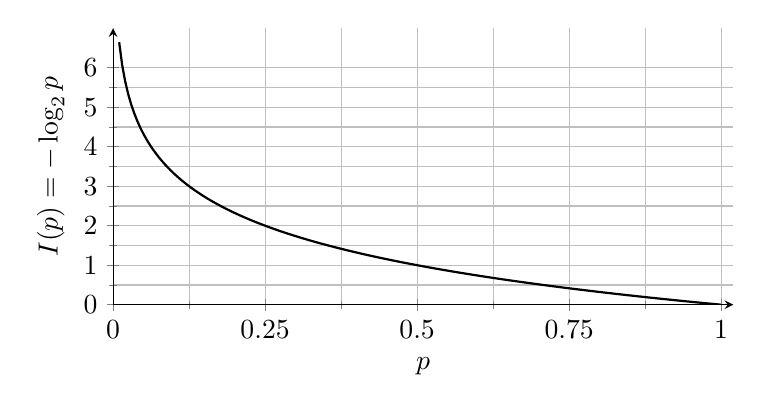
\begin{tikzpicture}
  \begin{axis}[
    width=0.78\textwidth,
    height=0.42\textwidth,
    domain=0.01:1,
    samples=200,
    axis lines=left,
    xmin=0, xmax=1.02,
    ymin=0, ymax=7,
    xlabel={$p$},
    ylabel={$I(p)=-\log_2 p$},
    xtick={0,0.25,0.5,0.75,1},
    ytick={0,1,2,3,4,5,6},
    grid=both,
    minor tick num=1,
  ]
    \addplot[thick] {-ln(x)/ln(2)};
  \end{axis}
\end{tikzpicture}

  \caption{Andamento del contenuto informativo \(I(p)=-\log_2 p\) al variare della probabilità \(p\).}
  \label{fig:fi-contenuto-informativo}
\end{figure}

Il contenuto informativo si misura in \emph{bit}: un esito tra due alternative
equiprobabili fornisce un bit, mentre un evento certo fornisce zero bit.
Per una sorgente con esiti di probabilità \(p_1,\ldots,p_r\), con
\(\sum_{i=1}^r p_i=1\), l'\emph{entropia di Shannon} è il contenuto
informativo medio:
\[
  H:=-\sum_{i=1}^{r}p_i\log_2p_i,
\]
con la convenzione \(0\log_2 0=0\). Il bit come unità di informazione va
distinto dalla cifra binaria \(0\) o \(1\), impiegata per rappresentare
i dati (\cref{sec:fi-conversioni-binarie}).\footnote{C. E. Shannon,
\emph{A Mathematical Theory of Communication}, \emph{Bell System
Technical Journal}, 1948.}

\clearpage

La teoria dell'informazione studia anche la trasmissione dei messaggi
attraverso canali soggetti a \emph{rumore}, che può alterare i dati
trasmessi. L'introduzione di \emph{ridondanza} mediante opportune
codifiche permette di rilevare e, in determinati casi, correggere
gli errori. La \emph{compressione} affronta invece il problema di
rappresentare l'informazione utilizzando meno simboli, sfruttando
le caratteristiche della sorgente.

La \cref{fig:fi-trasmissione-informazione} schematizza il percorso
del messaggio dalla sorgente alla destinazione, evidenziando
l'intervento del rumore durante la trasmissione.

\begin{figure}[htbp]
  \centering
  \resizebox{\linewidth}{!}{%
    
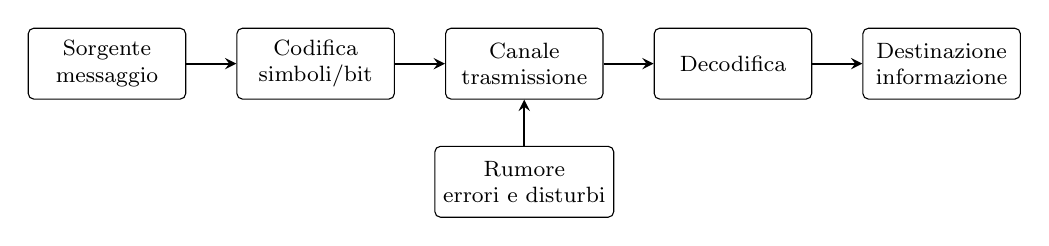
\begin{tikzpicture}[
  >=stealth,
  blocco/.style={
    draw,
    rounded corners=2pt,
    align=center,
    minimum width=2cm,
    minimum height=0.9cm,
    inner sep=3pt,
    font=\footnotesize
  },
  collegamento/.style={->, thick}
]

\node[blocco] (sorgente) at (0,0)
  {Sorgente\\messaggio};

\node[blocco] (codifica) at (2.65,0)
  {Codifica\\simboli/bit};

\node[blocco] (canale) at (5.3,0)
  {Canale\\trasmissione};

\node[blocco] (decodifica) at (7.95,0)
  {Decodifica};

\node[blocco] (destinazione) at (10.6,0)
  {Destinazione\\informazione};

\draw[collegamento] (sorgente.east) -- (codifica.west);
\draw[collegamento] (codifica.east) -- (canale.west);
\draw[collegamento] (canale.east) -- (decodifica.west);
\draw[collegamento] (decodifica.east) -- (destinazione.west);

\node[blocco] (rumore) at (5.3,-1.5)
  {Rumore\\errori e disturbi};

\draw[collegamento] (rumore.north) -- (canale.south);

\end{tikzpicture}
%
  }
  \caption{Schema della trasmissione dell'informazione: il messaggio
  viene codificato, trasmesso attraverso un canale soggetto a rumore
  e decodificato alla destinazione.}
  \label{fig:fi-trasmissione-informazione}
\end{figure}

Un \emph{calcolatore} è un dispositivo programmabile che memorizza dati,
esegue istruzioni e comunica con l'esterno. Le sue componenti fisiche
costituiscono l'\emph{hardware}; i programmi costituiscono il
\emph{software}. Una \emph{computazione} è un'elaborazione eseguita
secondo regole determinate, indipendentemente dal dispositivo utilizzato.
Fra i calcolatori rientrano anche sistemi integrati in oggetti e
ambienti, spesso collegati in rete: questa diffusione prende il nome di
\emph{informatica pervasiva}.

Un \emph{problema di calcolo} specifica gli ingressi ammissibili e il
risultato richiesto. Una particolare scelta dei dati di ingresso
costituisce un'\emph{istanza} del problema. Un \emph{algoritmo}
(\cref{def:fi-algoritmo}) descrive un procedimento risolutivo, mentre
un \emph{programma} ne costituisce un'implementazione in un linguaggio
di programmazione (ad esempio, Python e Java, trattati rispettivamente
nei \cref{chap:introduzione-python,chap:introduzione-java}).
La \emph{programmazione} comprende la progettazione, la scrittura e la
verifica del programma rispetto alle specifiche del problema.

\section{Algoritmi e risoluzione dei problemi}
\label{sec:fi-algoritmi}

\begin{definition}[Algoritmo]
\label{def:fi-algoritmo}
Un \emph{algoritmo} è un procedimento descritto mediante un numero finito
di istruzioni non ambigue ed effettivamente eseguibili, che termina dopo
un numero finito di passi per ogni ingresso ammissibile. Un algoritmo
risolve un problema se restituisce il risultato richiesto per ogni
ingresso previsto.
\end{definition}

L'eseguibilità, l'assenza di ambiguità e la terminazione sono condizioni
distinte dalla \emph{correttezza} del risultato. In particolare, la
finitezza della descrizione non garantisce la terminazione di una
ripetizione (si veda anche la \cref{sec:fi-ricorsione-terminazione}).
Inoltre, la specifica del problema deve stabilire criteri
verificabili: individuare il paesaggio «più rilassante», per esempio,
non definisce un problema di calcolo finché non viene precisato
come confrontare i paesaggi.

\clearpage

\begin{example}[Raddoppio di un capitale]
\label{ex:fi-interesse-composto}
Un capitale iniziale di \(20\,000\) euro produce un interesse annuo
costante del \(5\%\), capitalizzato alla fine di ogni anno. Senza
versamenti, prelievi o arrotondamenti intermedi, si vuole determinare
il primo anno in cui il saldo raggiunge almeno \(40\,000\) euro.

Il procedimento è il seguente:
\begin{enumerate}
  \item porre \(n=0\) e \(S=20\,000\);
  \item finché \(S<40\,000\), porre \(S=1{,}05S\) e \(n=n+1\);
  \item restituire \(n\).
\end{enumerate}
\end{example}

\begin{proof}[Verifica del procedimento]
Dopo \(n\) ripetizioni il saldo è
\[
  S_n=20\,000(1{,}05)^n.
\]
Finché la condizione del ciclo è vera, \(S_n\ge20\,000\) e l'aumento
annuo è almeno \(1\,000\) euro. L'algoritmo termina dunque in non più
di venti ripetizioni. Poiché la soglia è controllata prima di ogni
aggiornamento, il valore restituito è il primo anno richiesto.
In particolare,
\[
  S_{14}\approx39\,598{,}63<40\,000,
  \qquad
  S_{15}\approx41\,578{,}56>40\,000.
\]
Il risultato richiesto è quindi \(15\) anni.
\end{proof}

\begin{figure}[htbp]
  \begin{minipage}[c]{0.57\textwidth}
    Il ciclo dell'\cref{ex:fi-interesse-composto} è un esempio di
    ripetizione, che sarà esaminata nella \cref{sec:fi-python-cicli}.
    Il controllo di un algoritmo può essere rappresentato mediante un
    \emph{diagramma di flusso}: i rettangoli indicano le operazioni, i
    rombi le decisioni, gli ovali l'inizio e la fine, mentre le frecce
    indicano il passaggio fra istruzioni. Un diagramma descrive il flusso
    di controllo, ma non ne dimostra la correttezza. La
    \cref{fig:fi-diagramma-conteggio} ne mostra un esempio.
  \end{minipage}
  \hfill
  \begin{minipage}[c]{0.32\textwidth}
    \centering
    \resizebox{0.85\linewidth}{!}{%
      % Diagramma originale; licenza CC BY-SA 4.0 del materiale didattico.
\begin{tikzpicture}[unipd/diagram,node distance=7mm]
  \node[unipd/flow start] (inizio) {Inizio};
  \node[unipd/flow process,rounded corners=0pt,below=of inizio]
    (inizializzazione) {\(n\gets0\)};
  \node[unipd/flow decision,below=of inizializzazione]
    (condizione) {\(n<3\)?};
  \node[unipd/flow process,rounded corners=0pt,below=10mm of condizione]
    (incremento) {\(n\gets n+1\)};
  \node[unipd/flow end,below=of incremento] (fine) {Fine};
  \draw[unipd/flow arrow] (inizio) -- (inizializzazione);
  \draw[unipd/flow arrow] (inizializzazione) -- (condizione);
  \draw[unipd/flow arrow] (condizione) --
    node[unipd/edge label,midway,right,xshift=1mm,yshift=1mm] {Sì} (incremento);
  \draw[unipd/flow arrow] (incremento.west) -- ++(-6mm,0)
    |- (condizione.west);
  \draw[unipd/flow arrow] (condizione.east) --
    node[unipd/edge label,midway,above] {No} ++(9mm,0)
    |- (fine.east);
\end{tikzpicture}
%
    }
    \caption{Diagramma di flusso di un procedimento iterativo di conteggio.}
    \label{fig:fi-diagramma-conteggio}
  \end{minipage}
\end{figure}

L'esistenza di un algoritmo risolutivo riguarda la
\emph{calcolabilità} del problema, approfondita nella
\cref{sec:fi-macchina-turing}.
La \emph{complessità computazionale} riguarda invece le risorse
necessarie, principalmente tempo e memoria, in funzione della
dimensione dell'ingresso (\cref{chap:complessita}). Un problema può
essere calcolabile senza ammettere una soluzione praticabile con le
risorse disponibili.

\clearpage

\section{La macchina di Turing e i limiti del calcolo}
\label{sec:fi-macchina-turing}

Per precisare il concetto di procedimento effettivo si utilizza la
\emph{macchina di Turing}, un modello astratto introdotto nel 1936
nello studio dei fondamenti del calcolo. Il problema della decisione,
posto nel programma di Hilbert, chiedeva se esistesse un procedimento generale
per stabilire la validità delle formule della logica del primo ordine.
Church e Turing dimostrarono, con metodi diversi, che tale procedimento
non esiste.\footnote{L. De Mol,
\href{https://plato.stanford.edu/entries/turing-machine/}
{\emph{Turing Machines}}, \emph{Stanford Encyclopedia of Philosophy}.}

Una macchina di Turing deterministica comprende un nastro teoricamente
illimitato, suddiviso in celle, una testina di lettura e scrittura e
un controllo con un numero finito di stati. Una \emph{regola di
transizione} associa allo stato corrente e al simbolo letto il simbolo
da scrivere, lo spostamento della testina e lo stato successivo.
L'ingresso occupa inizialmente un tratto finito del nastro,
come illustrato nella \cref{fig:fi-nastro-turing}.

\begin{figure}[htbp]
  \centering
  % Diagramma originale; licenza CC BY-SA 4.0 del materiale didattico.
\begin{tikzpicture}[unipd/diagram]
  \foreach \i/\tapesymbol in {0/\mdlgwhtsquare,1/0,2/1,3/1,4/0,5/\mdlgwhtsquare,6/\mdlgwhtsquare} {
    \node[unipd/node,rectangle,rounded corners=0pt,
          minimum width=10mm,minimum height=10mm,inner sep=0pt]
      (cell\i) at (\i,0) {$\tapesymbol$};
  }
  \node at (-0.9,0) {$\cdots$};
  \node at (6.9,0) {$\cdots$};
  \node[unipd/node] (head) at (3,1.5) {Testina: stato $q$};
  \draw[unipd/directed edge,shorten <=2pt,shorten >=2pt]
    (head.south) -- (cell3.north);
  % Etichetta separata: il suo sfondo non deve coprire la freccia.
  \draw[unipd/edge,<->] (2,-0.9) -- (4,-0.9);
  \node[unipd/edge label] at (3,-1.4) {spostamento di una cella};
\end{tikzpicture}

  \caption{Nastro e testina di una macchina di Turing: \(q\) indica
  lo stato corrente e \(\mdlgwhtsquare\) il simbolo di bianco.}
  \label{fig:fi-nastro-turing}
\end{figure}

Una \emph{configurazione} è determinata dal contenuto del nastro,
dalla posizione della testina e dallo stato. L'esecuzione consiste
in una successione di configurazioni; può arrestarsi oppure proseguire
indefinitamente. Il nastro illimitato è un'idealizzazione e non
rappresenta la memoria di un calcolatore fisico.

Una \emph{macchina universale} riceve la descrizione codificata di
un'altra macchina e un ingresso, simulandone il comportamento.
L'universalità riguarda la possibilità di simulare ogni macchina
del modello, non la capacità di risolvere ogni problema.
La \emph{tesi di Church--Turing} afferma che i procedimenti
intuitivamente effettivi coincidono con quelli calcolabili da una
macchina di Turing. Collega così una nozione intuitiva a un modello
formale, senza costituire un teorema dimostrabile all'interno del modello.

\begin{definition}[Problema decidibile]
\label{def:fi-decidibilita}
Un \emph{problema di decisione} richiede una risposta «sì» oppure «no».
Si dice \emph{decidibile} se esiste un algoritmo che termina per ogni
ingresso ammissibile e restituisce sempre la risposta corretta;
altrimenti si dice \emph{indecidibile}.
\end{definition}

\begin{proposition}[Indecidibilità del problema dell'arresto]
\label{prop:fi-problema-arresto}
Non esiste un algoritmo che, ricevuti la descrizione di una macchina
di Turing arbitraria e un suo ingresso, termini sempre e stabilisca
correttamente se la macchina si arresterà su tale ingresso.
\end{proposition}

\begin{proof}
Si supponga per assurdo che esista un algoritmo \(O\) che termina
sempre e, ricevuti la descrizione \(p\) di un programma e un ingresso
\(x\), restituisca
\[
  O(p,x)=
  \begin{cases}
    1, & \text{se il programma \(p\) termina su \(x\)},\\
    0, & \text{se il programma \(p\) non termina su \(x\)}.
  \end{cases}
\]

Mediante \(O\) si costruisce un programma \(D\) che, ricevuta la
descrizione \(p\), si comporta nel modo seguente:
\[
  D(p):\quad
  \begin{cases}
    \text{esegue un ciclo infinito}, & \text{se } O(p,p)=1,\\
    \text{termina}, & \text{se } O(p,p)=0.
  \end{cases}
\]
Sia \(d\) la descrizione del programma \(D\) e si consideri
\(D(d)\). Si distinguono due casi.

\emph{Primo caso.}
Se \(O(d,d)=1\), l'algoritmo \(O\) dichiara che \(D(d)\) termina,
ma per costruzione \(D(d)\) non termina.

\emph{Secondo caso.}
Se \(O(d,d)=0\), l'algoritmo \(O\) dichiara che \(D(d)\) non termina,
ma per costruzione \(D(d)\) termina.

In entrambi i casi si ottiene una contraddizione. Pertanto un
algoritmo \(O\) con le proprietà supposte non esiste.
\end{proof}

La \cref{prop:fi-problema-arresto} esclude un decisore generale,
non la possibilità di verificare la terminazione di singoli programmi.
Questo limite di calcolabilità è distinto dai vincoli di tempo e
memoria studiati nel \cref{chap:complessita}.

\section{Architettura del calcolatore ed esecuzione delle istruzioni}
\label{sec:fi-architettura-calcolatore}

A differenza della macchina di Turing descritta nella
\cref{sec:fi-macchina-turing}, utilizzata per studiare i limiti
teorici del calcolo, l'\emph{architettura di von Neumann} descrive
l'organizzazione delle componenti di un calcolatore. In questo
modello, istruzioni e dati sono conservati nella stessa memoria,
alla quale la CPU accede mediante collegamenti condivisi.
Il \emph{principio del programma memorizzato} permette di eseguire
programmi diversi senza modificare i circuiti del calcolatore.

Nell'\emph{architettura Harvard}, invece, istruzioni e dati
sono conservati in memorie separate, accessibili attraverso
percorsi distinti. I processori moderni possono combinare
caratteristiche dei due modelli, mantenendo separati alcuni
percorsi di accesso pur utilizzando una memoria principale comune.

La \emph{CPU} (\emph{Central Processing Unit}) comprende l'\emph{unità
di controllo}, che coordina l'esecuzione, l'\emph{unità
logico-aritmetica} (ALU), che esegue operazioni aritmetiche e logiche,
e i \emph{registri}, che conservano temporaneamente dati e informazioni
di controllo. La CPU è realizzata mediante circuiti integrati a transistor
e può comprendere più \emph{core}, capaci di eseguire flussi di
istruzioni distinti. La \cref{fig:fi-von-neumann} schematizza
le componenti principali.

\begin{figure}[htbp]
  \centering
  \begin{tikzpicture}[unipd/diagram]
  \draw[unipd/edge,rounded corners=2pt] (-4.6,0.5) rectangle (4.6,2.7);
  \node at (0,2.4) {CPU};
  \node[unipd/architecture component] (control) at (-3,1.35)
    {Unità di\\controllo};
  \node[unipd/architecture component] (alu) at (0,1.35) {ALU};
  \node[unipd/architecture component] (registers) at (3,1.35)
    {Registri\\PC, istruzione\\dati};
  \draw[unipd/edge,<->] (control) -- (alu);
  \draw[unipd/edge,<->] (alu) -- (registers);
  \draw[unipd/edge,line width=1.2pt] (-4.6,-0.3) -- (4.6,-0.3);
  \node[font=\normalfont,anchor=north] at (0,-0.4)
    {Bus: dati, indirizzi, controllo};
  \draw[unipd/edge,<->] (0,0.5) -- (0,-0.3);
  \node[unipd/architecture component] (memory) at (-3,-1.5)
    {Memoria centrale\\istruzioni e dati};
  \node[unipd/architecture component] (io) at (3,-1.5)
    {Interfacce I/O\\periferiche};
  \draw[unipd/edge,<->] (memory.north) -- (-3,-0.3);
  \draw[unipd/edge,<->] (io.north) -- (3,-0.3);
\end{tikzpicture}

  \caption{Modello funzionale di von Neumann: CPU, memoria e
  dispositivi di ingresso e uscita.}
  \label{fig:fi-von-neumann}
\end{figure}

I \emph{bus} permettono lo scambio di informazioni fra le componenti.
Si distinguono, in base alla funzione, il \emph{bus dei dati}, che
trasferisce valori e istruzioni, il \emph{bus degli indirizzi}, che
identifica le locazioni interessate, e il \emph{bus di controllo},
che coordina le operazioni. Un collegamento condiviso semplifica
l'organizzazione e l'espansione del sistema, ma richiede di arbitrare
gli accessi e può costituire un \emph{collo di bottiglia} fra CPU e memoria.

\clearpage

Il registro \emph{program counter} (PC) contiene l'indirizzo della
prossima istruzione; il \emph{registro istruzione} conserva quella
prelevata. In un modello semplificato, l'esecuzione comprende quattro fasi:
\begin{enumerate}
  \item \emph{fetch}: prelievo dell'istruzione dalla memoria;
  \item \emph{decode}: identificazione dell'operazione e degli operandi;
  \item \emph{execute}: esecuzione dell'operazione;
  \item \emph{write-back}: eventuale scrittura del risultato.
\end{enumerate}
Il PC viene normalmente aggiornato all'indirizzo dell'istruzione
successiva; le istruzioni di salto possono invece modificarne il
contenuto, permettendo di realizzare condizioni e cicli nei programmi
(\cref{sec:fi-python-condizioni,sec:fi-python-cicli}).

Il \emph{clock} scandisce le operazioni delle componenti sincrone.
Per un segnale di periodo \(T\), la frequenza è \(f=1/T\) e si misura
in hertz. Un ciclo di clock non coincide necessariamente con
l'esecuzione completa di un'istruzione; la frequenza, da sola, non
ne determina le prestazioni.

Il \emph{parallelismo a livello di istruzioni} permette di
sovrapporre operazioni appartenenti a istruzioni diverse.
In una \emph{pipeline} ogni istruzione attraversa più stadi, che
possono operare contemporaneamente su istruzioni differenti,
come mostrato nella \cref{fig:fi-pipeline}.

\begin{figure}[htbp]
  \centering
  \begin{tikzpicture}[unipd/diagram,x=0.9cm,y=0.65cm]
  \node[anchor=east] at (-0.7,0) {Ciclo};
  \foreach \cycle in {1,...,8} {
    \node at (\cycle,0) {\cycle};
  }
  \foreach \instruction in {1,...,4} {
    \node[anchor=east] at (-0.7,-\instruction) {Istruzione \instruction};
    \foreach \stage/\name in {0/F,1/D,2/O,3/E,4/W} {
      \node[unipd/node,rounded corners=0pt,minimum width=8mm,
        minimum height=6mm,inner sep=0pt]
        at ({\instruction+\stage},-\instruction) {\name};
    }
  }
\end{tikzpicture}

  \caption{Pipeline ideale a cinque stadi: prelievo (F), decodifica (D),
  recupero operandi (O), esecuzione (E) e scrittura (W).}
  \label{fig:fi-pipeline}
\end{figure}

La pipeline aumenta idealmente il numero di istruzioni completate
per unità di tempo, non necessariamente la rapidità di ciascuna.
Dipendenze e conflitti sulle risorse possono introdurre attese.
Una \emph{CPU superscalare} dispone di più unità funzionali e può
avviare più istruzioni nello stesso ciclo, se le dipendenze lo
consentono. Pipeline e organizzazione superscalare sono compatibili.
Il parallelismo può inoltre coinvolgere più core o processori:
nei \emph{multiprocessori} più CPU condividono la memoria, mentre nei
\emph{multicalcolatori} i nodi hanno memorie proprie e comunicano
mediante messaggi.

Le \emph{GPU} (\emph{Graphics Processing Unit}) privilegiano
l'esecuzione parallela di numerose operazioni su dati diversi.
Rispetto alla CPU, che dedica maggiori risorse per core alla gestione
di flussi di controllo complessi, una GPU dispone di molte unità
di calcolo progettate per eseguire operazioni simili in parallelo.
Questa organizzazione è utile non soltanto per la grafica, ma anche
per simulazioni numeriche, elaborazione di immagini e addestramento
di reti neurali, quando il calcolo può essere suddiviso in molte
operazioni indipendenti.

\emph{CUDA} (\emph{Compute Unified Device Architecture}) è una
piattaforma NVIDIA nella quale la CPU (\emph{host}) prepara i dati
e avvia sulla GPU (\emph{device}) funzioni dette \emph{kernel}.
I \emph{thread} del kernel sono organizzati in \emph{blocchi},
raccolti in una \emph{griglia}. I thread di uno stesso blocco
possono collaborare mediante memoria condivisa e sincronizzazione.
I blocchi sono assegnati alle unità di esecuzione della GPU,
dette \emph{Streaming Multiprocessor}, che eseguono gruppi di thread
secondo il modello SIMT (\emph{Single Instruction, Multiple Threads}).

Il modello SIMT non implica che tutti i thread avanzino sempre
contemporaneamente: l'efficienza dipende dal grado di parallelismo,
dalle divergenze nel flusso di controllo e dai trasferimenti di dati.
Altri ambienti di calcolo eterogeneo includono ROCm/HIP, OpenCL,
SYCL, Vulkan Compute e Metal. Nei sistemi eterogenei possono inoltre
essere presenti acceleratori specializzati, come le \emph{NPU}
(\emph{Neural Processing Unit}), progettate per operazioni tipiche
delle reti neurali.

\section{Memoria, archiviazione e dispositivi di ingresso e uscita}
\label{sec:fi-memoria-archiviazione}

Nella rappresentazione dei dati, un \emph{bit} è una cifra binaria
che assume valore \(0\) oppure \(1\), e un \emph{byte} comprende otto
bit (\cref{chap:rappresentazione-informazioni}).

La memoria è suddivisa in \emph{locazioni}, individuate mediante
\emph{indirizzi}. Con \(a\) bit di indirizzo si possono distinguere
\(2^a\) locazioni. Se ogni locazione corrisponde a un byte,
\[
  a=16\ \Longrightarrow\ 2^{16}\,\mathrm{B}=64\,\mathrm{KiB},
  \qquad
  a=32\ \Longrightarrow\ 2^{32}\,\mathrm{B}=4\,\mathrm{GiB}.
\]
Questi valori indicano lo spazio teoricamente indirizzabile,
non necessariamente la quantità di RAM installata.

I prefissi decimali e binari non sono equivalenti:
\[
  1\,\mathrm{kB}=10^3\,\mathrm{B},
  \qquad
  1\,\mathrm{KiB}=2^{10}\,\mathrm{B},
\]
\[
  1\,\mathrm{GB}=10^9\,\mathrm{B},
  \qquad
  1\,\mathrm{GiB}=2^{30}\,\mathrm{B}.
\]

La \emph{memoria centrale} conserva istruzioni e dati in uso.
La \emph{RAM} (\emph{Random Access Memory}) è normalmente volatile.
Tra le principali tecnologie figurano SRAM e DRAM; a quest'ultima
appartengono le varianti sincrone SDRAM e DDR SDRAM.
La \emph{ROM} (\emph{Read-Only Memory}) è non volatile e viene
utilizzata per conservare il firmware; PROM, EPROM ed EEPROM si
distinguono per le possibilità di programmazione e cancellazione. Il
firmware di molti sistemi moderni risiede in memoria flash riscrivibile.

La RAM è comunemente montata su moduli DIMM; nei sistemi che lo
prevedono, la memoria \emph{ECC} permette di rilevare e correggere
determinati errori di memorizzazione. I moduli SIMM costituiscono
un formato precedente ai DIMM.

La \emph{memoria secondaria} conserva dati e programmi in modo
persistente. Durante l'esecuzione, programmi e dati necessari vengono
caricati nella RAM; le modifiche destinate a permanere devono essere
salvate su un supporto non volatile.

Un \emph{disco rigido} (HDD) registra dati su piatti magnetici,
organizzati in tracce e settori. Il tempo di accesso dipende anche
dallo spostamento della testina e dalla latenza di rotazione.
Un'\emph{unità a stato solido} (SSD) utilizza memoria flash NAND,
un \emph{controller} e collegamenti SATA oppure PCI Express con
protocollo NVMe. Le celle NAND conservano informazioni mediante
cariche elettriche e supportano un numero limitato di cicli di
programmazione e cancellazione. Per ridurre l'usura delle celle,
il controller distribuisce le scritture mediante una tecnica detta
\emph{wear leveling} e gestisce la correzione degli errori.
Gli SSD non hanno parti meccaniche in movimento e offrono generalmente
minori tempi di accesso rispetto agli HDD.

I \emph{nastri magnetici} sono supporti ad accesso sequenziale,
adatti a backup e archiviazione di grandi quantità di dati; fra le
famiglie impiegate figurano DLT e LTO. I \emph{supporti ottici},
come CD, DVD e Blu-ray, impiegano un laser per rilevare variazioni
della superficie o dello strato registrabile; nei dischi prestampati
si distinguono \emph{pit} e \emph{land}. Le capacità tipiche di un
disco a singolo strato sono circa 700 MB per un CD, 4,7 GB per un
DVD e 25 GB per un Blu-ray. I \emph{floppy disk} sono un precedente
esempio di memoria magnetica rimovibile.

\clearpage

Registri, \emph{cache}, RAM e memoria secondaria costituiscono la
\emph{gerarchia di memoria}, illustrata nella
\cref{fig:fi-gerarchia-memoria}. I livelli più vicini alla CPU sono
generalmente più veloci, meno capienti e più costosi per bit.
La cache conserva copie di dati e istruzioni e sfrutta due forme di
località, la cui presenza dipende dalla sequenza di accessi:
\begin{figure}[htbp]
  \begin{minipage}[c]{0.48\textwidth}
    \begin{itemize}
      \item \emph{località temporale}: un dato usato recentemente
            tende a essere richiesto di nuovo;
      \item \emph{località spaziale}: dopo l'accesso a una locazione
            tendono a essere richieste locazioni vicine.
    \end{itemize}
  \end{minipage}
  \hfill
  \begin{minipage}[c]{0.48\textwidth}
    \centering
    \resizebox{0.95\linewidth}{!}{%
      \begin{tikzpicture}[unipd/diagram,x=1cm,y=1cm]
  \filldraw[unipd/edge,fill=unipd-soft]
    (0,4.95) -- (-1.10,3.50) -- (1.10,3.50) -- cycle;
  \filldraw[unipd/edge,fill=unipd-accent!10]
    (-1.10,3.50) -- (-1.94,2.40) -- (1.94,2.40) -- (1.10,3.50) -- cycle;
  \filldraw[unipd/edge,fill=unipd-soft]
    (-1.94,2.40) -- (-2.78,1.30) -- (2.78,1.30) -- (1.94,2.40) -- cycle;
  \filldraw[unipd/edge,fill=unipd-accent!10]
    (-2.78,1.30) -- (-3.62,0.20) -- (3.62,0.20) -- (2.78,1.30) -- cycle;
  \node[font=\sffamily\footnotesize] at (0,3.88) {Registri};
  \node[font=\sffamily\footnotesize] at (0,2.95) {Cache};
  \node[font=\sffamily\footnotesize] at (0,1.85) {RAM};
  \node[font=\sffamily\footnotesize,align=center] at (0,0.75)
    {Memoria\\secondaria};
  \node[anchor=west,font=\sffamily\footnotesize] at (3.85,3.88)
    {$\approx 0{,}3\,\mathrm{ns}$};
  \node[anchor=west,font=\sffamily\footnotesize] at (3.85,2.95)
    {$\approx 1\text{--}10\,\mathrm{ns}$};
  \node[anchor=west,font=\sffamily\footnotesize] at (3.85,1.85)
    {$\approx 50\text{--}100\,\mathrm{ns}$};
  \node[anchor=west,font=\sffamily\footnotesize] at (3.85,0.75)
    {$\approx 100\,\mu\mathrm{s}\text{--}10\,\mathrm{ms}$};
\end{tikzpicture}
%
    }

    \captionof{figure}{Gerarchia di memoria e tempi di accesso indicativi;
    per la memoria secondaria si considerano SSD e HDD.}
    \label{fig:fi-gerarchia-memoria}
  \end{minipage}
\end{figure}

I dispositivi di \emph{ingresso e uscita} (I/O, \emph{Input/Output})
scambiano dati con l'esterno. Tastiera, mouse, microfono, scanner e
sensori sono dispositivi di ingresso; monitor, stampante e altoparlanti
di uscita. Touchscreen, schede di rete e unità di archiviazione
consentono operazioni in entrambe le direzioni.

Nell'\emph{I/O programmato} la CPU gestisce il trasferimento e può
controllare ripetutamente la disponibilità del dispositivo
(\emph{polling}). Gli \emph{interrupt} permettono invece alla
periferica di segnalare un evento, provocando l'esecuzione di una
procedura di servizio. Il \emph{DMA} (\emph{Direct Memory Access})
consente a un controller di trasferire dati fra memoria e periferiche
senza coinvolgere la CPU in ogni singola operazione. Questi
meccanismi possono essere impiegati congiuntamente.

La \emph{scheda madre} collega CPU, RAM e periferiche mediante
socket, slot, chipset e controller. Ospita o collega anche espansioni
PCI Express e dispositivi di memoria tramite SATA o M.2.
Le \emph{porte fisiche} collegano periferiche esterne: USB,
HDMI, DisplayPort, Ethernet e connettori audio svolgono funzioni
diverse; USB-C è una forma di connettore che può supportare
trasferimento dati, alimentazione e, quando previsto, video.
Le \emph{porte logiche} dei protocolli di rete sono invece
identificatori di servizi e non connettori fisici.

Il \emph{sistema operativo} gestisce le risorse del calcolatore
e fornisce l'ambiente necessario all'esecuzione dei programmi.
Coordina i processi, la memoria, i file e l'accesso alle periferiche,
oltre a gestire utenti e permessi. Nei sistemi multiprogrammati
più processi possono avanzare durante lo stesso intervallo di tempo,
alternandosi nell'utilizzo di un singolo core oppure eseguendo
in parallelo su core distinti.

\section{Linguaggi di programmazione e forme di esecuzione}
\label{sec:fi-linguaggi-esecuzione}

\begin{definition}[Linguaggio formale]
\label{def:fi-linguaggio-formale}
Sia \(\Sigma\) un alfabeto finito e sia \(\Sigma^*\) l'insieme
delle stringhe finite su \(\Sigma\), compresa la stringa vuota
\(\varepsilon\). Un \emph{linguaggio formale} è un sottoinsieme
\[
  L\subseteq\Sigma^*.
\]
\end{definition}

Una \emph{grammatica} specifica le stringhe di un linguaggio mediante
simboli terminali, simboli non terminali, un simbolo iniziale e
regole di produzione.

\clearpage

\begin{example}[Una grammatica formale]
Siano \(a,b\) simboli terminali e \(S\) il simbolo iniziale,
con le produzioni
\[
  S\to aSb,\qquad S\to ab.
\]
La grammatica genera \(ab,aabb,aaabbb,\ldots\), ossia le stringhe
\(a^nb^n\) con \(n\ge1\).
\end{example}

La \emph{gerarchia di Chomsky} distingue, in ordine di capacità
espressiva crescente, i linguaggi \emph{regolari}, \emph{liberi dal
contesto}, \emph{sensibili al contesto} e \emph{di tipo zero}.
I rispettivi modelli di riconoscimento sono gli automi finiti,
gli automi a pila non deterministici, gli automi linearmente
limitati non deterministici e le macchine di Turing.

Un \emph{riconoscitore} per un linguaggio \(L\) accetta ogni stringa
appartenente a \(L\); per una stringa non appartenente a \(L\)
può rifiutare oppure non terminare. Un \emph{decisore}, invece,
termina per ogni stringa, accettandola se appartiene a \(L\)
e rifiutandola altrimenti. Ogni decisore è quindi anche un
riconoscitore, ma non vale necessariamente il contrario
(\cref{def:fi-decidibilita}).

L'esecuzione di un programma dipende dall'\emph{insieme di istruzioni}
(\emph{instruction set}) supportato dal processore. Il
\emph{linguaggio macchina} ne rappresenta le codifiche binarie:
le categorie principali comprendono trasferimenti (\texttt{LOAD},
\texttt{STORE}), operazioni aritmetiche e logiche (\texttt{ADD},
\texttt{AND}) e salti incondizionati o condizionati
(\texttt{JUMP}, \texttt{JZ}), che modificano il PC.
Il \emph{linguaggio assembly} usa nomi mnemonici ed etichette
simboliche per istruzioni e indirizzi; un \emph{assemblatore} lo
traduce in codice macchina. L'insieme di istruzioni dipende
dall'architettura del processore.

I \emph{linguaggi ad alto livello}, come Python e Java, permettono
di descrivere operazioni senza specificare direttamente registri
e istruzioni della CPU. Il testo scritto dal programmatore è il
\emph{codice sorgente}; la \emph{sintassi} ne definisce le forme
ammesse, mentre la \emph{semantica} ne determina il significato.
Le regole sintattiche rigorose riducono le ambiguità che un traduttore
non potrebbe risolvere in modo affidabile interpretando le intenzioni
del programmatore. La correttezza sintattica non implica la
correttezza rispetto al problema (\cref{def:fi-algoritmo}).

Un \emph{compilatore} traduce il codice sorgente in codice macchina
o in un \emph{codice intermedio}; durante questa fase può segnalare
errori sintattici, senza garantire la correttezza dell'algoritmo.
Un \emph{interprete} esegue le operazioni previste dal linguaggio,
elaborando il sorgente o una rappresentazione intermedia.
I due meccanismi possono coesistere.

\begin{example}[Compilazione e interpretazione]
Un programma Java con una classe \texttt{Saluto} e un metodo
\texttt{main}, scritto nel file \texttt{Saluto.java}, può essere
compilato mediante \texttt{javac Saluto.java}, producendo il file
\texttt{Saluto.class}.
Quest'ultimo contiene \emph{bytecode} destinato alla
\emph{Java Virtual Machine} (JVM), che può interpretarlo oppure
tradurlo in codice macchina durante l'esecuzione mediante compilazione
\emph{Just-In-Time} (JIT).

In \emph{CPython}, il sorgente di un file \texttt{saluto.py}
viene tradotto in bytecode, successivamente eseguito dall'interprete.
In entrambi gli ambienti la traduzione e l'esecuzione sono fasi
distinte, e compilazione e interpretazione possono coesistere.
\end{example}

Se la traduzione produce codice macchina, può seguire il
\emph{collegamento} (\emph{linking}) con altri moduli e librerie;
il sistema operativo provvede poi al caricamento e all'avvio.
Lo stesso sorgente può essere compilato per architetture differenti,
ma l'\emph{eseguibile nativo} dipende dall'architettura e
dall'ambiente di destinazione.

L'esecuzione dei programmi Python è approfondita nella
\cref{sec:fi-python-esecuzione}, mentre la compilazione e
l'esecuzione dei programmi Java sono trattate nel
\cref{chap:introduzione-java}.

\chapter{Rappresentazione delle informazioni}
\label{chap:rappresentazione-informazioni}

Come anticipato nella \cref{sec:fi-informatica-calcolo}, un elaboratore
memorizza l'informazione mediante sequenze di bit. L'interpretazione
di una sequenza dipende dalla codifica adottata: gli stessi bit possono
rappresentare numeri, caratteri oppure altri dati.\footnote{Materiale di riferimento:
S. Canazza, \emph{Rappresentazione delle informazioni},
\nolinkurl{2026_FI_01_canazza_RappresentazioneInformazioni.pdf}.}

\section{Sistemi di numerazione posizionali}
\label{sec:fi-notazione-posizionale}

Nei sistemi di numerazione \emph{posizionali} il valore di una cifra dipende
dalla sua posizione e dalla base. Il sistema decimale impiega le cifre da
\(0\) a \(9\); quello binario le cifre \(0\) e \(1\). Nelle scritture posizionali si usa il punto come separatore
frazionario e il pedice per indicare la base.

\begin{definition}[Valore posizionale]
\label{def:fi-valore-posizionale}
Siano \(b\ge2\) una base intera e \(a_k\in\{0,\ldots,b-1\}\) le cifre di
una rappresentazione con \(n\ge1\) cifre intere e \(m\ge0\) cifre
frazionarie. Il valore della scrittura
\[
  (a_{n-1}\cdots a_0.a_{-1}\cdots a_{-m})_b
\]
è
\[
  x=\sum_{k=0}^{n-1}a_kb^k+\sum_{j=1}^{m}a_{-j}b^{-j}.
\]
Per \(m=0\) la seconda somma è nulla e il separatore si omette.
\end{definition}

\begin{example}[Pesi delle cifre decimali]
Applicando il valore posizionale alle cifre decimali si ottiene
\begin{align*}
  (753)_{10}&=7\cdot10^2+5\cdot10+3=753,\\
  (2048)_{10}&=2\cdot10^3+4\cdot10+8=2048,\\
  (4.34)_{10}&=4+3\cdot10^{-1}+4\cdot10^{-2}.
\end{align*}
\end{example}

\section{Notazione binaria e conversioni}
\label{sec:fi-conversioni-binarie}

Il \emph{bit} (\emph{binary digit}) è una cifra binaria. La base due è
adatta ai circuiti digitali, nei quali è possibile distinguere due stati
logici. La conversione da binario a decimale si ottiene applicando la
\cref{def:fi-valore-posizionale}.

\begin{example}[Da binario a decimale]
La somma dei pesi delle cifre binarie fornisce
\begin{align*}
  (1101)_2&=2^3+2^2+1=13,\\
  (1.101)_2&=1+2^{-1}+2^{-3}=1.625.
\end{align*}
\end{example}

Viceversa, per convertire un numero decimale non negativo in binario
si trattano separatamente la parte intera e quella frazionaria.

\subsection{Divisioni successive per la parte intera}

Sia \(N\in\N\), con la convenzione \(0\in\N\). Per \(N>0\), si divide
ripetutamente per due, ottenendo quozienti \(q_i\) e resti \(r_i\):
\[
  q_0=N,\qquad q_i=2q_{i+1}+r_i,
  \qquad r_i\in\{0,1\}.
\]
Quando il quoziente diventa zero, la sequenza binaria è formata dai resti
letti \emph{in ordine inverso}. Infatti, sostituendo successivamente i
quozienti si ricava
\[
  N=r_0+2r_1+\cdots+2^{t-1}r_{t-1}.
\]
Per \(N=0\) la rappresentazione è \(0\).

\begin{example}[Conversione di cento]
Applicando le divisioni successive a \(100\) si ottiene
\begin{alignat*}{3}
  100&=2\cdot50+0, &\quad 50&=2\cdot25+0, &\quad25&=2\cdot12+1,\\
  12&=2\cdot6+0, & 6&=2\cdot3+0, & 3&=2\cdot1+1,\\
  1&=2\cdot0+1.
\end{alignat*}
Leggendo i resti dal basso verso l'alto,
\[
  (100)_{10}=(1100100)_2=2^6+2^5+2^2.
\]
\end{example}

\subsection{Moltiplicazioni successive per la parte frazionaria}

Sia \(f_0\in[0,1)\). Si moltiplica ripetutamente la frazione per due:
\[
  2f_{j-1}=d_j+f_j,
  \qquad d_j\in\{0,1\},\quad f_j\in[0,1).
\]
Le parti intere \(d_j\) forniscono i bit frazionari, letti
\emph{nell'ordine di produzione}. Dopo \(t\) passi,
\[
  f_0=\sum_{j=1}^{t}d_j2^{-j}+f_t2^{-t}.
\]
La conversione termina se \(f_t=0\); se una frazione residua si ripete,
la sequenza di bit è periodica da quel punto.

\begin{example}[Frazione binaria finita]
La conversione di \(0.625\) richiede tre moltiplicazioni successive:
\[
  0.625\cdot2=1+0.25,\qquad
  0.25\cdot2=0+0.5,\qquad
  0.5\cdot2=1.
\]
Pertanto \((0.625)_{10}=(0.101)_2\).
\end{example}

\begin{example}[Frazione binaria periodica]
\label{ex:fi-frazione-periodica}
Per \(0.35=7/20\) si ottiene
\begin{align*}
  2\cdot0.35&=0+0.70, & 2\cdot0.70&=1+0.40,\\
  2\cdot0.40&=0+0.80, & 2\cdot0.80&=1+0.60,\\
  2\cdot0.60&=1+0.20, & 2\cdot0.20&=0+0.40.
\end{align*}
Poiché \(0.40\) ricompare, il periodo è \(0110\). Quindi
\[
  (0.35)_{10}=(0.01\overline{0110})_2,
  \qquad
  (100.35)_{10}=(1100100.01\overline{0110})_2.
\]
\end{example}

\begin{proposition}[Frazioni con rappresentazione binaria finita]
\label{prop:fi-frazione-binaria-finita}
Una frazione \(p/q\in[0,1)\), ridotta ai minimi termini e con \(q>0\),
ammette una rappresentazione binaria finita se e solo se \(q\) è una
potenza di due.
\end{proposition}

\begin{proof}
Una scrittura con \(m\) cifre frazionarie ha valore \(K/2^m\), quindi
il denominatore ridotto divide \(2^m\). Viceversa, se \(q=2^h\), bastano
al più \(h\) cifre. Negli altri casi i resti della conversione assumono
soltanto un numero finito di valori non nulli: uno si ripete e la
rappresentazione è periodica da una certa posizione.
\end{proof}

\section{Numeri senza segno e modulo e segno}
\label{sec:fi-interi-rappresentazione}

Fissata una lunghezza di \(n\ge1\) bit, si hanno \(2^n\) configurazioni.
Nell'interpretazione \emph{senza segno}, la sequenza \(a_{n-1}\cdots a_0\) vale
\[
  U=\sum_{k=0}^{n-1}a_k2^k,
  \qquad U\in[0,2^n-1]\cap\Z.
\]
Con otto bit si rappresentano quindi gli interi da \(0\) a \(255\).
Il bit più a sinistra è detto \emph{più significativo} (MSB); quello
più a destra \emph{meno significativo} (LSB).

\begin{definition}[Modulo e segno]
Per \(n\ge2\), nella rappresentazione con \emph{modulo e segno} il bit
più significativo \(s\) indica il segno, mentre gli altri \(n-1\) bit
rappresentano il modulo \(M\):
\[
  a=(-1)^sM,\qquad
  M=\sum_{k=0}^{n-2}a_k2^k.
\]
\end{definition}

Le sequenze \(001100\) e \(101100\) su sei bit rappresentano
rispettivamente \(+12\) e \(-12\). L'intervallo dei valori è
\[
  [-(2^{n-1}-1),\,2^{n-1}-1]\cap\Z.
\]
Le configurazioni sono \(2^n\), ma i valori distinti sono \(2^n-1\):
\(00\cdots0\) e \(10\cdots0\) rappresentano entrambe zero.
Inoltre, la somma richiede di distinguere operandi con segno uguale,
per i quali si sommano i moduli mantenendo il segno comune, e con
segno opposto, per i quali si sottrae il modulo minore da quello
maggiore, attribuendo al risultato il segno dell'operando di
modulo maggiore. Se i moduli sono uguali e i segni opposti,
il risultato è zero.

\section{Complemento a due}
\label{sec:fi-complemento-due}

Il \emph{complemento a due} evita la doppia rappresentazione dello zero
e permette di eseguire le somme di interi con segno mediante
l'addizione binaria su \(n\) bit, purché il risultato sia rappresentabile.

\begin{definition}[Codifica in complemento a due]
\label{def:fi-complemento-due}
Sia \(n\ge2\). Per ogni intero
\[
  a\in[-2^{n-1},2^{n-1}-1]\cap\Z,
\]
la codifica in complemento a due è la rappresentazione senza segno
su \(n\) bit di
\[
  C_n(a)=
  \begin{cases}
    a, & a\ge0,\\
    a+2^n, & a<0.
  \end{cases}
\]
\end{definition}

Per decodificare una sequenza di valore senza segno \(U\), si pone
\[
  a=\begin{cases}
    U, & U<2^{n-1},\\
    U-2^n, & U\ge2^{n-1}.
  \end{cases}
\]
Equivalentemente, il bit più significativo ha peso negativo:
\begin{equation}
  a=-a_{n-1}2^{n-1}+\sum_{k=0}^{n-2}a_k2^k.
  \label{eq:fi-pesi-complemento-due}
\end{equation}

Il bit più significativo indica quindi il segno, ma gli altri bit di
un numero negativo non ne rappresentano il modulo. Gli estremi
sono \(-2^{n-1}\) e \(2^{n-1}-1\); su otto bit si ha
\([-128,127]\cap\Z\) e su trentadue bit
\([-2147483648,2147483647]\cap\Z\), intervallo del tipo
\texttt{int} di Java, i cui estremi sono disponibili mediante
\texttt{Integer.MIN\_VALUE} e \texttt{Integer.MAX\_VALUE}
(\cref{sec:fi-java-tipi-fondamentali}).

\subsection{Codifica, inversione e decodifica}

Per ottenere la codifica di \(-m\) su \(n\) bit, con
\(1\le m\le2^{n-1}\), si calcola \(2^n-m\). Equivalentemente, si
scrive \(m\) su \(n\) bit, si invertono tutti i bit e si aggiunge uno.
Infatti, l'inversione produce \(2^n-1-m\).

\begin{example}[Un intero negativo su otto bit]
Per \(-13\) si ha
\[
  2^8-13=243=(1111\,0011)_2.
\]
Anche l'inversione con incremento fornisce
\[
  0000\,1101\longrightarrow1111\,0010
  \xrightarrow{+1}1111\,0011.
\]
Dall'\cref{eq:fi-pesi-complemento-due} segue
\[
  -128+64+32+16+2+1=-13.
\]
Analogamente, \(-14\) corrisponde a \(1111\,0010\).
\end{example}

\begin{warning}[Il formato determina il valore]
\label{warn:fi-larghezza-interi}
La sequenza \(1111\,1111\) rappresenta \(255\) senza segno, \(-127\)
con modulo e segno e \(-1\) in complemento a due su otto bit. In
complemento a due su sedici bit, \(0000\,0000\,1111\,1111\) vale
invece \(+255\). È necessario specificare formato e larghezza.
\end{warning}

Nell'\emph{estensione del segno} si replica il bit più significativo
per aumentare la larghezza senza cambiare il valore. Per esempio,
\(1111\,0011\) su otto bit rappresenta \(-13\); la sua estensione
a sedici bit è
\[
  (1111\,1111\,1111\,0011)_2.
\]
La negazione di \(-2^{n-1}\) non è rappresentabile con \(n\)
bit in complemento a due.

\clearpage

\section{Aritmetica intera e overflow}
\label{sec:fi-aritmetica-overflow}

L'addizione binaria conserva \(n\) bit e scarta il riporto finale:
il risultato è la somma delle codifiche \emph{modulo} \(2^n\).
Nella colonna \(k\), con riporto entrante \(c_k\), vale
\[
  a_k+b_k+c_k=r_k+2c_{k+1},\qquad c_0=0.
\]
Se la somma matematica non appartiene all'intervallo rappresentabile,
si verifica \emph{overflow} (trabocco).

\begin{example}[Riporto scartato senza overflow]
Su otto bit,
\[
  \begin{array}{r@{\;}r}
      &0000\,0101\\
    + &1111\,1110\\ \hline
    1 &0000\,0011
  \end{array}
\]
rappresenta \(5+(-2)=3\). Il riporto finale viene scartato, ma
non si verifica overflow con segno.
\end{example}

\begin{proposition}[Criterio di overflow nell'addizione]
\label{prop:fi-overflow-somma}
Nella somma di due interi su \(n\) bit in complemento a due,
si verifica overflow se e solo se gli operandi hanno lo stesso segno
e il risultato ha segno opposto. Equivalentemente, il riporto
entrante nel bit di segno \(c_{n-1}\) è diverso dal riporto uscente
\(c_n\).
\end{proposition}

\begin{proof}
La somma di interi con segno opposto è compresa fra gli operandi e non
può eccedere l'intervallo disponibile. La somma di due non negativi
può superare solo il massimo e produrre un bit di segno uguale a uno;
quella di due negativi può scendere sotto il minimo e produrre un
bit di segno nullo. Applicando la regola dell'addizione alla colonna di
segno, i due casi corrispondono rispettivamente a
\((c_{n-1},c_n)=(1,0)\) e \((0,1)\).
\end{proof}

\begin{example}[Overflow positivo e negativo su quattro bit]
L'intervallo è \([-8,7]\cap\Z\). Si ha
\[
  0110+0010=1000,\qquad 1101+1001=1\,0110.
\]
Nel primo caso \(6+2=8\) produce \(-8\); nel secondo
\((-3)+(-7)=-10\) produce \(+6\) dopo lo scarto del riporto.
Entrambi i risultati sono corretti modulo \(16\), ma non come
somme di interi con segno.
\end{example}

\section{Virgola fissa e virgola mobile}
\label{sec:fi-virgola-mobile}

Con \(n\) bit si distinguono soltanto \(2^n\) configurazioni, quindi
non tutti i numeri reali sono rappresentabili esattamente. Alcune
frazioni, tuttavia, hanno una scrittura binaria finita, come mostrato
nella \cref{sec:fi-conversioni-binarie}.

Nella rappresentazione in \emph{virgola fissa} la posizione del
separatore è prestabilita. Usando \(n\) bit senza segno, di cui
\(0\le m\le n\) frazionari, si rappresentano valori \(U2^{-m}\), con
\(0\le U\le2^n-1\), distanziati di \(2^{-m}\).

Nella rappresentazione in \emph{virgola mobile} un numero finito non
nullo è espresso nella forma
\[
  x=(-1)^sM\,b^E,
\]
dove \(s\) indica il segno, \(M\) è il \emph{significando} (o
\emph{mantissa}) ed \(E\) l'esponente. La \emph{normalizzazione}
richiede \(1\le M<b\). In base due, per esempio,
\[
  (10.5)_{10}=(1010.1)_2=(1.0101)_2\cdot2^3.
\]
Il numero di cifre significative determina la precisione, mentre
l'esponente determina l'ordine di grandezza.

\subsection{I formati IEEE 754 binary32 e binary64}
\label{sec:fi-ieee754}

Lo standard IEEE 754 definisce, fra gli altri, i formati \emph{binary32}
e \emph{binary64}, rispettivamente a singola e doppia precisione.\footnote{
Oracle, \emph{Numerical Computation Guide},
\href{https://docs.oracle.com/cd/E19957-01/806-3568/ncg_math.html}{capitolo 2, IEEE Arithmetic}.}
Ciascuno comprende un bit di segno \(s\), un campo per l'esponente e
uno per la frazione. I parametri sono riportati nella
\cref{tab:fi-formati-ieee}.

\begin{table}[htbp]
  \centering
  \begin{tabular}{lcc}
    \toprule
    Parametro & binary32 & binary64 \\
    \midrule
    Bit complessivi & 32 & 64 \\
    Segno & 1 & 1 \\
    Esponente \(w\) & 8 & 11 \\
    Frazione \(t\) & 23 & 52 \\
    Bias \(B\) & 127 & 1023 \\
    Bit significativi normali & 24 & 53 \\
    Esponenti normali & \(-126\) a \(127\) & \(-1022\) a \(1023\) \\
    \bottomrule
  \end{tabular}
  \caption{Parametri dei formati IEEE 754 binari.}
  \label{tab:fi-formati-ieee}
\end{table}

Sia \(e\) il valore intero senza segno del campo esponente e \(F\)
quello del campo frazione. Il \emph{bias} \(B=2^{w-1}-1\) permette di
codificare gli esponenti senza usare il complemento a due: per i
numeri normali l'esponente effettivo è \(E=e-B\). I campi
\(e=0\) ed \(e=2^w-1\) sono riservati.

\begin{definition}[Valori normali e subnormali]
\label{def:fi-valori-ieee}
Nei formati della \cref{tab:fi-formati-ieee}, per
\(1\le e\le2^w-2\) il valore \emph{normale} è
\[
  x=(-1)^s\left(1+\frac{F}{2^t}\right)2^{e-B}.
\]
Per \(e=0\) e \(F\ne0\), il valore \emph{subnormale} è
\[
  x=(-1)^s\frac{F}{2^t}\,2^{1-B}.
\]
\end{definition}

Il bit iniziale \(1\) del significando normale è implicito;
nei subnormali il bit iniziale è invece \(0\).

\begin{example}[Codifica di un valore normale]
Il numero \(10.5=(1.0101)_2\cdot2^3\), codificato in binary32,
ha \(s=0\), \(e=3+127=130=(10000010)_2\) e frazione
\(0101\) seguita da diciannove zeri:
\[
  \underbrace{0}_{s}\quad
  \underbrace{10000010}_{e}\quad
  \underbrace{01010000000000000000000}_{\text{frazione}}.
\]
La decodifica restituisce \((1+2^{-2}+2^{-4})2^3=10.5\).
\end{example}

\clearpage

\subsection{Valori limite, zeri e configurazioni speciali}

Per i formati della \cref{tab:fi-formati-ieee}, il minimo normale
positivo, il minimo subnormale positivo e il massimo finito positivo
sono rispettivamente
\[
  2^{1-B},\qquad
  2^{1-B-t},\qquad
  (2-2^{-t})2^{2^w-2-B}.
\]
In binary32 valgono
\begin{align*}
  x_{\min,\mathrm{norm}}&=2^{-126}\approx1.1755\cdot10^{-38},\\
  x_{\min,\mathrm{sub}}&=2^{-149}\approx1.4013\cdot10^{-45},\\
  x_{\max}&=(2-2^{-23})2^{127}\approx3.4028\cdot10^{38}.
\end{align*}

In binary64 valgono
\begin{align*}
  x_{\min,\mathrm{norm}}&=2^{-1022}\approx2.2251\cdot10^{-308},\\
  x_{\min,\mathrm{sub}}&=2^{-1074}\approx4.9407\cdot10^{-324},\\
  x_{\max}&=(2-2^{-52})2^{1023}\approx1.7977\cdot10^{308}.
\end{align*}

I subnormali consentono un \emph{underflow graduale} verso zero,
con una precisione relativa decrescente.

Le configurazioni riservate sono riepilogate nella
\cref{tab:fi-valori-speciali}.

\begin{table}[htbp]
  \centering
  \begin{tabular}{lll}
    \toprule
    Esponente & Frazione & Valore \\
    \midrule
    \(e=0\) & \(F=0\) & \(+0\) oppure \(-0\) \\
    \(e=0\) & \(F\ne0\) & Subnormale \\
    \(1\le e\le2^w-2\) & Qualsiasi \(F\) & Normale \\
    \(e=2^w-1\) & \(F=0\) & \(+\infty\) oppure \(-\infty\) \\
    \(e=2^w-1\) & \(F\ne0\) & NaN \\
    \bottomrule
  \end{tabular}
  \caption{Interpretazione dei campi IEEE 754.}
  \label{tab:fi-valori-speciali}
\end{table}

\emph{NaN} (\emph{Not a Number}) rappresenta risultati non numerici,
come \(0/0\) e \(+\infty-(+\infty)\) nell'aritmetica IEEE 754.
Un confronto di uguaglianza con NaN è falso anche quando si confronta
NaN con sé stesso. Il comportamento delle operazioni e la segnalazione
degli errori dipendono anche dal linguaggio e dall'ambiente: in Python,
per esempio, \texttt{1.0/0.0} solleva \texttt{ZeroDivisionError}.

\section{Precisione e arrotondamento}
\label{sec:fi-precisione-arrotondamento}

Per i numeri normali positivi nell'intervallo
\([2^E,2^{E+1})\), la distanza fra valori consecutivi è
\[
  \delta_E=2^{E-t},
\]
dove \(t\) è il numero di bit della frazione (\cref{tab:fi-formati-ieee}).
In binary32 il passo è \(1\) in corrispondenza di \(2^{23}\) e
\(16\) in corrispondenza di \(2^{27}\). Nei subnormali il passo
resta \(2^{1-B-t}\).

Se un risultato non è rappresentabile esattamente, viene
\emph{arrotondato}. La modalità predefinita IEEE 754 è
\emph{al più vicino, con parità in caso di equidistanza}
(\emph{ties to even}); sono previste anche le modalità verso zero,
verso \(+\infty\) e verso \(-\infty\). L'aritmetica a precisione
finita distingue l'errore di rappresentazione degli operandi da quello
di arrotondamento del risultato.

\begin{example}[Il valore decimale \(4.35\)]
\label{ex:fi-arrotondamento-prodotto}
La parte frazionaria di \(4.35\) è \(0.35=7/20\) e, per la
\cref{prop:fi-frazione-binaria-finita}, non ammette una
rappresentazione binaria finita.
In binary64, arrotondato al più vicino, vale
\[
  \widehat{x}\approx4.3499999999999996.
\]
La moltiplicazione, arrotondata nello stesso formato, produce
\[
  \operatorname{fl}(\widehat{x}\cdot100)
  =435-2^{-44}\approx434.99999999999994,
\]
anziché \(435\). In binary32, invece, il prodotto arrotondato
è \(435\): l'esito dipende dal formato.
\end{example}

\begin{example}[Allineamento degli esponenti e perdita di cifre]
Allineando gli esponenti dei due addendi si ottiene
\begin{align*}
  10.5+0.125
    &=(1.0101)_2\cdot2^3+(1.0)_2\cdot2^{-3}\\
    &=\bigl((1.0101)_2+(0.000001)_2\bigr)2^3\\
    &=(1.010101)_2\cdot2^3=10.625.
\end{align*}
Il risultato richiede sette bit significativi; in binary32 e binary64
è esatto. In un formato didattico con cinque bit significativi e
arrotondamento al più vicino, il passo presso \(10.5\) è \(0.5\):
la somma viene arrotondata a \(10.5\).
\end{example}

Un addendo piccolo può dunque non modificare il valore memorizzato.
Inoltre, l'addizione in virgola mobile non è, in generale, associativa:
le approssimazioni possono variare con l'ordine delle operazioni.

\section{Notazione esadecimale e ottale}
\label{sec:fi-esadecimale-ottale}

Per scrivere più concisamente le sequenze binarie si utilizza la
base sedici, che impiega le cifre
\(0,\ldots,9,\mathrm{A},\ldots,\mathrm{F}\),
con \(\mathrm{A}=10,\ldots,\mathrm{F}=15\). Poiché \(16=2^4\),
una cifra esadecimale corrisponde a quattro bit. I gruppi si formano
partendo dal separatore: verso sinistra per la parte intera e verso
destra per quella frazionaria.

\begin{example}[Raggruppamento in base sedici]
Raggruppando i bit in gruppi di quattro si ottiene
\begin{align*}
  (0111\,1111)_2&=(\mathrm{7F})_{16}=127,\\
  (1011\,0110)_2&=(\mathrm{B6})_{16}=182,\\
  (1101.101)_2&=(1101.1010)_2=(\mathrm{D.A})_{16}=13.625.
\end{align*}
Nell'ultimo esempio si aggiunge uno zero a destra della parte
frazionaria. La notazione \texttt{0x7F} indica comunemente
\((\mathrm{7F})_{16}\).
\end{example}

La base otto impiega le cifre da \(0\) a \(7\). Poiché \(8=2^3\),
una cifra ottale corrisponde a tre bit. I gruppi si formano
partendo dal separatore: verso sinistra per la parte intera e verso
destra per quella frazionaria.

\clearpage

\begin{example}[Raggruppamento in base otto]
Raggruppando i bit in gruppi di tre si ottiene
\begin{align*}
  (100010)_2&=(100\,010)_2=(42)_8=34,\\
  (11100010)_2&=(011\,100\,010)_2=(342)_8=226,\\
  (1101.101)_2&=(001\,101.101)_2=(15.5)_8=13.625.
\end{align*}
Nell'ultimo esempio si aggiungono due zeri a sinistra della parte
intera. In Python, la notazione \texttt{0o42} indica
\((42)_8\).
\end{example}

Nelle conversioni inverse si sostituisce ogni cifra esadecimale con
quattro bit e ogni cifra ottale con tre bit. La base non determina
il segno: per interpretare una sequenza come intero con segno occorre
conoscere il formato (\cref{warn:fi-larghezza-interi}).

\section{Rappresentazione dei caratteri}
\label{sec:fi-caratteri}

Per rappresentare un testo si associano codici numerici ai suoi
caratteri. Un \emph{punto di codice} è un valore numerico che può
essere assegnato a un carattere del repertorio; il
\emph{formato di codifica} ne stabilisce la rappresentazione in
memoria. Uno stesso punto di codice può quindi avere
rappresentazioni in byte diverse.

\subsection{ASCII e codifiche a otto bit}

Il codice \emph{ASCII} (\emph{American Standard Code for Information
Interchange}) usa sette bit e comprende \(128\) codici, da \(0\) a
\(127\). I codici \(0\)--\(31\) e \(127\) sono di controllo;
i codici \(32\)--\(126\) sono stampabili.

\begin{table}[htbp]
  \centering
  \begin{tabular}{lll}
    \toprule
    Codice & Simbolo & Significato \\
    \midrule
    9 & \texttt{\textbackslash t} & Tabulazione orizzontale (HT) \\
    10 & \texttt{\textbackslash n} & Nuova riga (LF) \\
    13 & \texttt{\textbackslash r} & Ritorno a inizio riga (CR) \\
    32 & Spazio & Spazio \\
    48--57 & \texttt{0}--\texttt{9} & Cifre decimali \\
    65--90 & \texttt{A}--\texttt{Z} & Lettere maiuscole \\
    97--122 & \texttt{a}--\texttt{z} & Lettere minuscole \\
    127 & \texttt{DEL} & Carattere di controllo \\
    \bottomrule
  \end{tabular}
  \caption{Codici e intervalli ASCII principali.}
  \label{tab:fi-ascii}
\end{table}

I codici di \texttt{0} e \texttt{1} sono rispettivamente \(48\) e
\(49\), distinti dai valori numerici zero e uno. Le sequenze
\texttt{\textbackslash n}, \texttt{\textbackslash r} e
\texttt{\textbackslash t} sono notazioni impiegate nei linguaggi di
programmazione per indicare caratteri di controllo.

ASCII non comprende le lettere accentate. La denominazione
\emph{ASCII esteso} indica diverse codifiche a otto bit, non uno
standard unico: ISO-8859-1 e Windows-1252, per esempio, condividono
i primi \(128\) codici, ma assegnano significati differenti ad alcuni
byte successivi.

\subsection{Unicode e formati UTF}

\emph{Unicode} assegna ai caratteri punti di codice indicati con
il prefisso \texttt{U+}, seguito da almeno quattro cifre
esadecimali. Lo spazio dei punti di codice arriva a
\texttt{U+10FFFF}; i primi \(128\) corrispondono ad ASCII.
Unicode non prescrive due byte per carattere e non tutti i punti
di codice sono assegnati.\footnote{Unicode Consortium,
\emph{The Unicode Standard},
\href{https://www.unicode.org/versions/Unicode17.0.0/core-spec/chapter-2/}{capitolo 2}.}
L'intervallo \texttt{U+D800}--\texttt{U+DFFF} è riservato ai surrogati.

I formati principali sono \emph{UTF-8}, che impiega da uno a quattro
byte, \emph{UTF-16}, che impiega una o due unità di sedici bit, e
\emph{UTF-32}, che impiega un'unità di trentadue bit. In UTF-8
le sequenze ASCII restano invariate. UTF-16 utilizza coppie di
surrogati per i punti di codice superiori a \texttt{U+FFFF};
per la memorizzazione delle unità su più byte occorre specificare
l'ordine dei byte.

\begin{example}[Punto di codice e byte memorizzati]
La lettera \texttt{A}, punto di codice \texttt{U+0041}, occupa
il byte \texttt{41} in UTF-8. La lettera \texttt{è}, punto di
codice \texttt{U+00E8}, occupa \texttt{C3 A8} in UTF-8,
\texttt{00 E8} in UTF-16BE e \texttt{E8 00} in UTF-16LE.
In ISO-8859-1 occupa invece il byte \texttt{E8}.
\end{example}

Un carattere visualizzato può comprendere più punti di codice:
numero di caratteri, punti di codice e byte non coincidono
necessariamente.

\chapter{Introduzione a Python}
\label{chap:introduzione-python}

Un algoritmo può essere tradotto in un programma mediante un linguaggio di
programmazione (\cref{sec:fi-algoritmi,sec:fi-linguaggi-esecuzione}). In questo
capitolo si considera Python 3, non pienamente compatibile con Python 2,
e se ne introducono le istruzioni fondamentali per gestire i dati,
controllare il flusso di esecuzione e organizzare il codice.\footnote{Materiale
di riferimento: S. Canazza, \emph{Python},
\nolinkurl{2026_FI_02_canazza_Python.pdf}.}

\section{Python e l'esecuzione dei programmi}
\label{sec:fi-python-esecuzione}

Python è un linguaggio \emph{ad alto livello} e \emph{general purpose}. Un
programma può essere salvato in un file sorgente, generalmente con estensione
\texttt{.py}, ed eseguito mediante un interprete. Nell'implementazione
CPython, il sorgente viene tradotto in \emph{bytecode}, poi eseguito
dalla macchina virtuale Python. La distinzione fra compilazione e
interpretazione è richiamata nella \cref{sec:fi-linguaggi-esecuzione}.

La funzione \texttt{print()} scrive sull'uscita standard. Una \emph{stringa}
è una sequenza di caratteri, delimitata nel codice da apici singoli o doppi;
il carattere \texttt{\#}, fuori dalle stringhe, introduce un commento fino
al termine della riga.

\begin{unipdcode}[language=Python]
# Un messaggio sul terminale
print("Ciao, mondo!")
\end{unipdcode}


Salvato il sorgente come \texttt{saluto.py}, lo si può eseguire dal
terminale:

\begin{unipdterminal}
$ python3 saluto.py
Ciao, mondo!
\end{unipdterminal}


Il nome del comando può essere \texttt{python} oppure
\texttt{python3}, a seconda dell'ambiente;
\verb|python3 --version| ne mostra la versione.
Gli esempi richiedono Python 3.9 o successivo.
Il simbolo \texttt{\$} nel terminale identifica il prompt e non fa parte
del comando.

Avviando l'interprete senza indicare un file si accede invece alla modalità
interattiva, riconoscibile dal prompt \lstinline|>>>|. Questa modalità
segue il ciclo \emph{REPL} (\emph{Read, Eval, Print, Loop}): valuta ogni
istruzione inserita e mostra il risultato delle espressioni, quando
previsto. In uno script, invece, le espressioni non vengono stampate
automaticamente.

\section{Variabili, tipi di dato e ingresso/uscita}
\label{sec:fi-python-variabili}

Per riutilizzare i valori durante l'esecuzione si impiegano le variabili.
L'\emph{assegnamento} associa un nome al valore di un'espressione:
\texttt{prezzo = 10} assegna \texttt{10} a \texttt{prezzo};
\texttt{prezzo = prezzo + 1} ne aggiorna il valore utilizzando quello
precedente. L'operatore \texttt{=} non indica quindi l'uguaglianza
matematica. Il riferimento a un nome non ancora definito provoca
\texttt{NameError}.

Per scambiare i valori di due variabili senza perdere quelli originali
si può utilizzare una variabile temporanea, eseguendo in sequenza
gli assegnamenti \texttt{tmp = a}, \texttt{a = b} e \texttt{b = tmp}.
Python permette anche l'assegnamento
multiplo \texttt{a, b = b, a}, nel quale le espressioni a destra vengono
valutate prima di effettuare gli assegnamenti. Nel caso di valori interi,
lo scambio può essere realizzato anche mediante tre operazioni XOR
bit a bit: \verb|a ^= b|, \verb|b ^= a|, \verb|a ^= b|,
sfruttando la proprietà \(x \oplus x = 0\).

I nomi delle variabili, detti \emph{identificatori}, possono contenere
lettere, cifre e il carattere \texttt{\_}, ma non iniziare con una cifra.
Distinguono maiuscole e minuscole e non possono coincidere con parole
riservate, come \texttt{if} e \texttt{for}. Per i nomi composti si adotta
generalmente la convenzione \emph{snake\_case}, ad esempio
\texttt{prezzo\_unitario} (un'altra convenzione è \emph{camelCase},
utilizzata generalmente in Java per variabili e metodi;
\cref{sec:fi-java-identificatori}).

In Python il tipo appartiene al valore, non al nome: un nome può essere
riassegnato a valori di tipi diversi. I tipi fondamentali sono
\texttt{int} per gli interi, \texttt{float} per i numeri in virgola mobile,
\texttt{str} per le stringhe e \texttt{bool} per i valori
\texttt{True} e \texttt{False}. La funzione \texttt{type()} restituisce
il tipo di un valore. Gli \texttt{int} non hanno una larghezza fissa,
mentre le approssimazioni dei \texttt{float} dipendono dalla
rappresentazione descritta nella
\cref{sec:fi-precisione-arrotondamento}.

Gli operatori \texttt{+}, \texttt{-}, \texttt{*} e \texttt{**} indicano
rispettivamente somma, sottrazione, prodotto e potenza. Per la divisione
si distinguono:
\[
\begin{array}{rcl@{\qquad}l}
  \texttt{17 / 5}  &=& 3.4 & \text{divisione ordinaria},\\
  \texttt{17 // 5} &=& 3 & \text{quoziente arrotondato verso }-\infty,\\
  \texttt{17 \% 5}  &=& 2 & \text{resto della divisione}.
\end{array}
\]
La divisione \texttt{/} produce un valore \texttt{float} anche quando il
quoziente è intero. La potenza precede la moltiplicazione, che precede
l'addizione; le parentesi permettono di stabilire esplicitamente l'ordine
delle operazioni.

Il significato degli operatori dipende dai tipi degli operandi: per le
stringhe, \texttt{+} esegue la concatenazione, mentre la moltiplicazione
per un intero ne ripete il contenuto. Ad esempio,
\lstinline|"3" + "4"| produce \lstinline|"34"|, non \texttt{7};
tentare di sommare direttamente una stringa e un intero provoca
\texttt{TypeError}. Le funzioni \texttt{int()}, \texttt{float()}, \texttt{str()} e
\texttt{bool()} eseguono conversioni esplicite: \texttt{int(3.9)}
restituisce \texttt{3} (troncamento verso zero), mentre una conversione
impossibile, come \lstinline|int("ciao")|, genera \texttt{ValueError}.

La conversione \texttt{bool()} restituisce \texttt{False} per zero,
stringhe e liste vuote e \texttt{None}; per esempio,
\texttt{bool(0)} è \texttt{False} e \texttt{bool(3)} è
\texttt{True}. Il valore \texttt{None}, unico elemento del tipo
\texttt{NoneType}, rappresenta l'assenza di un valore.

La funzione \texttt{input()} legge una riga dall'ingresso standard e
restituisce una stringa, anche se l'utente ha digitato un numero.
Per eseguire calcoli occorre quindi convertire i valori acquisiti.

\begin{unipdcode}[language=Python]
primo = int(input("Primo intero: "))
secondo = int(input("Secondo intero: "))

# Si assume che le stringhe inserite rappresentino interi validi.
totale = primo
totale = totale + secondo
print("Somma:", totale)
print("Media:", totale / 2)
\end{unipdcode}

\clearpage

\section{Logica booleana e istruzioni condizionali}
\label{sec:fi-python-condizioni}

Per esprimere le condizioni che regolano il flusso di esecuzione si
utilizzano espressioni booleane. Gli operatori di confronto
\texttt{==}, \texttt{!=}, \texttt{<}, \texttt{<=}, \texttt{>} e
\texttt{>=} restituiscono valori booleani.
In particolare, \texttt{==} verifica l'uguaglianza, mentre \texttt{=}
esegue un assegnamento.

Gli operatori logici \texttt{and}, \texttt{or} e \texttt{not} esprimono
congiunzione, disgiunzione e negazione. Nelle seguenti tabelle di verità,
\(\mathrm{V}\) e \(\mathrm{F}\) indicano rispettivamente
\texttt{True} e \texttt{False}:
\[
\begin{array}{cc|cc}
  a & b & a\mathbin{\texttt{ and }}b & a\mathbin{\texttt{ or }}b\\
  \hline
  \mathrm{F} & \mathrm{F} & \mathrm{F} & \mathrm{F}\\
  \mathrm{F} & \mathrm{V} & \mathrm{F} & \mathrm{V}\\
  \mathrm{V} & \mathrm{F} & \mathrm{F} & \mathrm{V}\\
  \mathrm{V} & \mathrm{V} & \mathrm{V} & \mathrm{V}
\end{array}
\qquad
\begin{array}{c|c}
  a & \texttt{not }a\\
  \hline
  \mathrm{F} & \mathrm{V}\\
  \mathrm{V} & \mathrm{F}
\end{array}
\]
Le tabelle si riferiscono a operandi booleani. Più in generale, in
Python \texttt{and} e \texttt{or} restituiscono uno degli operandi,
non necessariamente un valore di tipo \texttt{bool}: il risultato
dipende dal valore di verità degli operandi. L'operatore \texttt{not}
restituisce invece sempre un valore booleano.

Fra gli operatori considerati, i confronti hanno precedenza su
\texttt{not}, che precede \texttt{and}, seguito da \texttt{or}.
Le \emph{leggi di De Morgan} forniscono le equivalenze
\[
\begin{aligned}
 \texttt{not (a and b)}&\quad\Longleftrightarrow\quad
 \texttt{(not a) or (not b)},\\
 \texttt{not (a or b)}&\quad\Longleftrightarrow\quad
 \texttt{(not a) and (not b)}.
\end{aligned}
\]
Gli operatori \texttt{and} e \texttt{or} usano la
\emph{valutazione a cortocircuito}, da sinistra verso destra:
il secondo operando viene valutato soltanto se il primo è
rispettivamente vero o falso. Perciò, in
\lstinline|x != 0 and 10 / x > 2|, la divisione non viene eseguita
quando \texttt{x} vale zero.

L'istruzione \texttt{if} esegue un blocco quando la condizione è vera;
\texttt{elif} introduce condizioni successive e \texttt{else} il caso
residuo. In una catena condizionale viene eseguito soltanto il blocco
associato alla prima condizione soddisfatta. Analogamente, \texttt{match},
disponibile da Python 3.10, seleziona il primo \texttt{case} applicabile,
senza richiedere \texttt{break}.

\begin{unipdcode}[language=Python]
voto = 27
if voto < 18:
    print("Insufficiente")
elif voto < 24:
    print("Sufficiente")
elif voto < 28:
    print("Buono")
else:
    print("Ottimo")
\end{unipdcode}


L'\emph{indentazione} identifica i blocchi di istruzioni ed è parte
della sintassi di Python. Dopo i due punti, le istruzioni del blocco
sono rientrate allo stesso livello; terminato il blocco, si ritorna
all'indentazione precedente. La convenzione è utilizzare quattro spazi
per livello. Un rientro non valido può produrre \texttt{IndentationError};
un rientro sintatticamente valido ma errato può invece modificare la
logica del programma.

\clearpage

\section{Cicli e iterazioni}
\label{sec:fi-python-cicli}

Le istruzioni condizionali selezionano il blocco da eseguire; un
\emph{ciclo} permette invece di ripeterlo. Ogni esecuzione del blocco
è detta \emph{iterazione}. Il ciclo \texttt{while} controlla una condizione
prima di ogni iterazione e termina quando essa diventa falsa. Il corpo
può quindi non essere eseguito neppure una volta. Diversamente, il ciclo
\texttt{do...while} verifica la condizione dopo l'esecuzione del corpo,
garantendo almeno un'iterazione. Quest'ultimo non è previsto direttamente in Python,
ma può essere simulato mediante \texttt{while True} e \texttt{break}.

\begin{unipdcode}[language=Python]
eta = int(input("Eta non negativa: "))
while eta < 0:
    eta = int(input("Valore non valido, riprovare: "))
print("Eta accettata:", eta)
\end{unipdcode}


L'esempio richiede nuovamente l'età finché il valore è negativo. La
terminazione dipende dall'inserimento di un intero non negativo; una
stringa non convertibile provocherebbe \texttt{ValueError}. Un ciclo
\texttt{while} può non terminare se la condizione rimane sempre vera.

Nei \emph{cicli con contatore} si distinguono inizializzazione,
condizione e aggiornamento. L'istruzione \texttt{n += 1} abbrevia
\texttt{n = n + 1}. Nei \emph{cicli con sentinella}, invece, un valore
prestabilito segnala la fine dell'acquisizione e non viene elaborato come
dato.

\begin{unipdcode}[language=Python]
somma = 0
numero = int(input("Numero (0 per terminare): "))
while numero != 0:
    somma += numero
    numero = int(input("Numero (0 per terminare): "))
print("Somma:", somma)
\end{unipdcode}


L'inserimento di zero termina il ciclo senza contribuire alla somma;
se è il primo valore, la somma resta nulla.

Il ciclo \texttt{for} visita, nell'ordine, i valori di un oggetto
\emph{iterabile}, assegnandoli alla variabile indicata. La funzione
\texttt{range()} fornisce una sequenza di interi con estremo iniziale
incluso ed estremo finale escluso:
\[
\begin{array}{ll}
  \texttt{range(5)} & 0,1,2,3,4,\\
  \texttt{range(2,6)} & 2,3,4,5,\\
  \texttt{range(0,10,2)} & 0,2,4,6,8,\\
  \texttt{range(5,0,-1)} & 5,4,3,2,1.
\end{array}
\]
Con tre argomenti \texttt{range(inizio, fine, passo)}, il passo può
essere negativo, ma non nullo. Il ciclo \texttt{for} non richiede
l'aggiornamento manuale della variabile di iterazione.

\begin{unipdcode}[language=Python]
totale = 0
for numero in range(1, 6):
    totale = totale + numero
print("Somma:", totale)
\end{unipdcode}


La variabile \texttt{totale} è un \emph{accumulatore}: contiene la somma
parziale e viene aggiornata a ogni iterazione. In questo caso il ciclo
somma gli interi da uno a cinque, individuati da \texttt{range(1, 6)},
ottenendo \texttt{15}. La funzione \texttt{sum()} permette di ottenere
lo stesso risultato mediante un'espressione generatrice:

\begin{unipdcode}[language=Python]
totale = sum(numero for numero in range(1, 6))
print("Somma:", totale)
\end{unipdcode}

La ricorsione fornisce un'altra forma di ripetizione del calcolo,
trattata nella \cref{sec:fi-ricorsione-terminazione}.

\section{Liste}
\label{sec:fi-python-liste}

I cicli possono elaborare anche sequenze di dati. Una \emph{lista} è
una sequenza modificabile di elementi, scritta nel codice tra
parentesi quadre. Gli elementi possono avere tipi differenti e sono
individuati dalla loro posizione, a partire dall'indice zero.
\texttt{len(lista)} restituisce il numero di elementi:
per una lista di lunghezza \(n\), gli indici non negativi validi sono
\(0,\ldots,n-1\). Gli indici negativi permettono di accedere agli
elementi dalla fine: \texttt{lista[-1]} indica l'ultimo,
\texttt{lista[-2]} il penultimo e \texttt{lista[-n]} il primo,
quando tali posizioni esistono. Un indice non valido provoca \texttt{IndexError}.

L'assegnamento \texttt{lista[i] = valore} modifica un elemento.
Il metodo \texttt{append(valore)} aggiunge un elemento in fondo,
\texttt{insert(i, valore)} lo inserisce nella posizione indicata,
\texttt{pop(i)} rimuove e restituisce l'elemento nella posizione
indicata oppure l'ultimo se l'indice è omesso, mentre
\texttt{remove(valore)} rimuove la prima occorrenza del valore
specificato. L'operatore \texttt{in} verifica la presenza di un valore.

Lo \emph{slicing} \texttt{lista[i:j]} estrae una nuova lista con estremo
iniziale incluso e finale escluso. Se l'estremo iniziale è omesso,
lo slicing parte dall'inizio; se è omesso quello finale, arriva fino
alla fine della lista. A differenza delle liste, le stringhe non sono
modificabili mediante assegnamento a un indice.

\texttt{sorted(lista)} restituisce una nuova lista ordinata senza
modificare quella originale, se gli elementi sono confrontabili;
\texttt{lista.sort()} ordina invece la lista stessa e restituisce
\texttt{None}. Gli algoritmi impiegati per ordinare i dati sono
studiati nel \cref{chap:ricerca-ordinamento}.

\begin{unipdcode}[language=Python]
voti = [20, 30, 27]
voti[0] = 21
voti.append(18)
ultimo = voti.pop()
ordinati = sorted(voti)
print("Primi due:", voti[:2])
print("Presente 30:", 30 in voti)

totale = 0
conteggio = 0
for voto in voti:
    if voto >= 24:
        totale = totale + voto
        conteggio = conteggio + 1
if conteggio > 0:
    print("Media dei voti almeno 24:", totale / conteggio)
\end{unipdcode}


Nell'esempio, \texttt{pop()} rimuove l'ultimo voto e
\texttt{sorted()} crea una copia ordinata. Il ciclo calcola la media
dei voti rimasti non inferiori a \texttt{24};
\texttt{if conteggio > 0} evita la divisione per zero.

\clearpage

\section{Funzioni}
\label{sec:fi-python-funzioni}

Per organizzare operazioni riutilizzabili si impiegano le \emph{funzioni},
che associano un nome a un blocco di istruzioni. Una funzione si definisce
mediante \texttt{def}. La definizione non esegue il corpo della
funzione: questo viene eseguito soltanto quando essa è \emph{chiamata}.
Prima della chiamata deve essere stata eseguita la definizione,
affinché il nome della funzione sia disponibile. I nomi dichiarati
nella definizione sono i
\emph{parametri}; i valori forniti alla chiamata
sono gli \emph{argomenti}. È possibile specificare annotazioni di tipo per
i parametri e per il valore restituito. L'intestazione di una funzione può
assumere la forma
\[
  \text{\texttt{def somma(a: int, b: int) -> int:}}
\]
Le annotazioni non impongono controlli automatici sui tipi durante
l'esecuzione. Una \emph{funzione annidata} è definita all'interno
di un'altra funzione: viene creata durante l'esecuzione di quella
esterna, ne può utilizzare le variabili locali ed è normalmente
accessibile soltanto nel suo ambito. L'esempio seguente ne mostra
l'impiego nel calcolo dell'area di un rettangolo.

\begin{unipdcode}[language=Python]
def area_rettangolo(base: int, altezza: int) -> int:
    def calcola_area() -> int:
        return base * altezza

    return calcola_area()


risultato = area_rettangolo(8, 5)
print("Area:", risultato)
\end{unipdcode}


L'istruzione \texttt{return} termina la chiamata e restituisce un
valore al chiamante; \texttt{print()} scrive invece sull'uscita
standard. Una funzione che termina senza \texttt{return} restituisce
\texttt{None}. I parametri e le variabili assegnate nel corpo sono
di norma \emph{locali} alla chiamata. Una funzione può anche
restituire un booleano, per esempio con
\texttt{return numero \% 2 == 0}.

Le definizioni possono essere raccolte in \emph{moduli}, ossia file
Python importabili. Salvando la definizione di
\texttt{area\_rettangolo} in \texttt{geometria.py}, un secondo file
può utilizzarla così:

\begin{unipdcode}[language=Python]
import geometria

print("Area:", geometria.area_rettangolo(8, 5))
\end{unipdcode}


Con \texttt{import geometria} si accede alla funzione mediante
\texttt{geometria.area\_rettangolo(8, 5)};
\lstinline|from geometria import area_rettangolo| rende disponibile
anche la chiamata diretta \lstinline|area_rettangolo(8, 5)|.
La parola \texttt{as} permette di assegnare un alias, per esempio
\lstinline|from geometria import area_rettangolo as area|.
Il nome del modulo si indica senza l'estensione \texttt{.py}.

Le funzioni possono anche richiamare se stesse, come si vedrà
nel \cref{chap:ricorsione}.

\clearpage

\section{Gestione dei file di testo}
\label{sec:fi-python-file}

Oltre al codice organizzato in moduli, un programma può utilizzare file
per conservare dati tra esecuzioni successive. I file sono memorizzati
nella memoria di massa (\cref{sec:fi-memoria-archiviazione}). In un
\emph{file di testo}, i byte vengono interpretati come caratteri
secondo una codifica, come UTF-8 (\cref{sec:fi-caratteri}); un
\emph{file binario} viene invece trattato come una sequenza di byte,
senza decodifica testuale automatica. In Python si distinguono le modalità
di apertura testuali da quelle binarie, indicate per esempio con
\lstinline|"rb"| e \lstinline|"wb"|.
Quando il nome non contiene un percorso assoluto, il file viene
cercato nella directory di lavoro corrente,
che non coincide necessariamente con quella del programma.

La funzione \texttt{open()} apre il file. Le modalità principali sono
\lstinline|"r"| per leggere, \lstinline|"w"| per creare o sovrascrivere
e \lstinline|"a"| per aggiungere dati in fondo. La modalità
\lstinline|"w"| cancella il contenuto preesistente all'apertura;
\lstinline|"r"| richiede invece che il file esista.

Il costrutto \texttt{with open(...) as file:} chiude il file
all'uscita dal blocco, anche se si verifica un errore. È opportuno
specificare la codifica UTF-8 mediante il parametro \texttt{encoding}.

\begin{unipdcode}[language=Python]
with open("voti.txt", "w", encoding="utf-8") as file:
    file.write("24\n27\n")

with open("voti.txt", "a", encoding="utf-8") as file:
    file.write("30\n")
\end{unipdcode}


Il metodo \texttt{write()} scrive una stringa senza aggiungere
automaticamente un fine riga; la sequenza \lstinline|"\n"| rappresenta
un carattere di nuova riga. L'esempio produce il file \texttt{voti.txt}
contenente tre interi, uno per riga. La prima apertura in modalità
\lstinline|"w"| sovrascrive eventuali dati precedenti; la seconda,
in modalità \lstinline|"a"|, aggiunge l'ultima riga.

Il metodo \texttt{read()} restituisce l'intero contenuto del file
come stringa. In alternativa, un ciclo \texttt{for} permette di leggerlo
\emph{riga per riga}; ogni riga contiene normalmente anche il
carattere di fine riga. \texttt{strip()} rimuove spazi bianchi iniziali
e finali, compresi i terminatori di riga. Un numero letto da un file
rimane testo finché non viene convertito con \texttt{int()} o
\texttt{float()}.

\begin{unipdcode}[language=Python]
try:
    totale = 0
    with open("voti.txt", "r", encoding="utf-8") as file:
        for riga in file:
            totale = totale + int(riga.strip())
    print("Somma:", totale)
except FileNotFoundError:
    print("File voti.txt non trovato.")
\end{unipdcode}


Il programma stampa \texttt{Somma: 81} se il file contiene i tre
valori dell'esempio precedente. La clausola
\texttt{except FileNotFoundError} gestisce l'assenza del file quando
questo viene aperto in lettura; contenuti non convertibili in interi
provocherebbero invece \texttt{ValueError}.

\chapter{Ricorsione}
\label{chap:ricorsione}

Le funzioni introdotte nella \cref{sec:fi-python-funzioni} possono
richiamare se stesse per risolvere un problema attraverso sottoproblemi
della stessa natura. Questa tecnica prende il nome di \emph{ricorsione}
e richiede di individuare un caso base e di ricavare la soluzione dai
risultati delle chiamate ricorsive.\footnote{Materiale
di riferimento: S. Canazza, \emph{Ricorsione}, file
\nolinkurl{2026_FI_03_canazza_Ricorsione.pdf}.}

\section{Funzioni ricorsive e terminazione}
\label{sec:fi-ricorsione-terminazione}

\begin{definition}[Ricorsione]
Una funzione è \emph{ricorsiva} se può invocare se stessa durante la
propria esecuzione. Un \emph{caso base} fornisce un risultato senza
ulteriori invocazioni ricorsive; un \emph{passo ricorsivo} esprime la
soluzione mediante uno o più sottoproblemi della stessa natura.
\end{definition}

Una chiamata ricorsiva avvia una nuova invocazione della funzione, con
parametri propri, mentre l'invocazione corrente rimane sospesa.
La presenza di un caso base non garantisce, da sola, la terminazione:
per ogni ingresso ammissibile, ciascuna successione di chiamate deve
raggiungere un caso base.

Un criterio sufficiente consiste nell'associare a ogni sottoproblema
una misura intera non negativa, strettamente decrescente a ogni
chiamata ricorsiva. Poiché non esistono successioni infinite strettamente
decrescenti di interi non negativi, ogni catena di chiamate raggiunge
un caso base, purché ciascuna invocazione esegua un numero finito
di operazioni non ricorsive e generi un numero finito di chiamate.
La terminazione, richiesta dalla \cref{def:fi-algoritmo}, non basta
a garantire la correttezza: occorre inoltre che i casi base e la
combinazione dei risultati forniscano la soluzione prevista.

\section{Il fattoriale: iterazione e ricorsione}
\label{sec:fi-fattoriale}

Per \(n\in\N\), il \emph{fattoriale} è definito dal prodotto
\(n!=1\cdot2\cdots n\), con \(0!=1\). Equivalentemente,
\begin{equation}
  n!=\begin{cases}
    1, & n=0,\\
    n(n-1)!, & n>0.
  \end{cases}
  \label{eq:fi-fattoriale}
\end{equation}

La definizione precedente si traduce nelle due implementazioni
seguenti, che calcolano lo stesso risultato per un intero non negativo:
la prima utilizza un ciclo (\cref{sec:fi-python-cicli}), la seconda
una chiamata ricorsiva.

\noindent\hspace*{2mm}%
\begin{minipage}[t]{\dimexpr\linewidth/2-4mm\relax}
\vspace{0pt}
\textbf{Versione iterativa}
\begin{unipdcode}[language=Python,
  basicstyle=\ttfamily\scriptsize,
  numbers=none,
  xleftmargin=0pt,
  xrightmargin=0pt,
  framexleftmargin=0.3em]
def fattoriale_iterativo(n):
    if n < 0:
        raise ValueError(
            "n deve essere non negativo"
        )
    risultato = 1
    for i in range(1, n + 1):
        risultato = risultato * i
    return risultato
\end{unipdcode}
\end{minipage}%
\hspace*{4mm}%
\begin{minipage}[t]{\dimexpr\linewidth/2-4mm\relax}
\vspace{0pt}
\textbf{Versione ricorsiva}
\begin{unipdcode}[language=Python,
  basicstyle=\ttfamily\scriptsize,
  numbers=none,
  xleftmargin=0pt,
  xrightmargin=0pt,
  framexleftmargin=0.3em]
def fattoriale(n):
    if n < 0:
        raise ValueError(
            "n deve essere non negativo"
        )
    if n == 0:
        return 1
    return n * fattoriale(n - 1)
\end{unipdcode}
\end{minipage}


Nella prima funzione, dopo l'iterazione di indice \(i\), la variabile
\texttt{risultato} vale \(i!\). Nella seconda, il caso base restituisce
\(0!=1\), mentre il passo ricorsivo applica l'\cref{eq:fi-fattoriale}.
La misura \(n\) diminuisce di uno a ogni chiamata e raggiunge zero.
La correttezza segue dalla stessa relazione: se la chiamata con \(n-1\)
restituisce \((n-1)!\), quella con \(n\) restituisce \(n!\).

\begin{unipdterminal}
>>> fattoriale(0), fattoriale(4)
(1, 24)
>>> fattoriale_iterativo(5), fattoriale(5)
(120, 120)
\end{unipdterminal}

Entrambe le funzioni presuppongono un argomento di tipo \texttt{int}.
Per \(n<0\) sollevano \texttt{ValueError}; senza tale controllo,
la versione ricorsiva non raggiungerebbe il caso base e, in CPython,
terminerebbe con \texttt{RecursionError}.

\section{Invocazioni sospese e pila delle chiamate}
\label{sec:fi-pila-ricorsione}

Per descrivere l'esecuzione ricorsiva occorre considerare anche le
invocazioni non ancora terminate. Quando una funzione ne invoca un'altra,
la prima sospende la propria esecuzione fino al ritorno della seconda.
Ogni invocazione mantiene un
\emph{record di attivazione}, o \emph{frame}, contenente parametri,
variabili locali e informazioni necessarie a riprendere il calcolo.
Le invocazioni ancora attive costituiscono la \emph{pila delle chiamate}
(\emph{call stack}), organizzata secondo l'ordine LIFO
(\emph{Last In, First Out}), proprio dell'ADT pila (\cref{sec:fi-adt-pila}).

\begin{example}[Traccia di \texttt{fattoriale(4)}]
\label{ex:fi-traccia-fattoriale}
Per valutare \texttt{fattoriale(4)}, le invocazioni con argomenti
\(4,3,2,1\) rimangono sospese fino al caso base \(n=0\), che restituisce
uno. Le chiamate riprendono quindi in ordine inverso:
\[
\begin{aligned}
  \texttt{fattoriale(0)}&=1,\\
  \texttt{fattoriale(1)}&=1\cdot1=1,\\
  \texttt{fattoriale(2)}&=2\cdot1=2,\\
  \texttt{fattoriale(3)}&=3\cdot2=6,\\
  \texttt{fattoriale(4)}&=4\cdot6=24.
\end{aligned}
\]
\end{example}

\begin{figure}[htbp]
  \centering
  \begin{tikzpicture}[unipd/diagram,x=1cm,y=1cm]
  \node at (0,0.65) {Chiamate};
  \node at (6,0.65) {Ritorni};
  \foreach \n/\y/\result in {4/0/24,3/-1/6,2/-2/2,1/-3/1,0/-4/1} {
    \node[unipd/node,minimum width=32mm] (c\n) at (0,\y)
      {\texttt{fattoriale(\n)}};
    \node[unipd/node,minimum width=32mm] (r\n) at (6,\y)
      {\(n=\n\): restituisce \(\result\)};
  }
  \foreach \n/\m in {4/3,3/2,2/1,1/0} {
    \draw[unipd/directed edge] (c\n) -- (c\m);
    \draw[unipd/directed edge] (r\m) -- (r\n);
  }
  \foreach \y/\text in {0/{\(4\cdot6=24\)},-1/{\(3\cdot2=6\)},-2/{\(2\cdot1=2\)},-3/{\(1\cdot1=1\)}} {
    \node at (3,\y) {\text};
  }
  \draw[unipd/directed edge] (c0) -- node[above] {Caso base: \(0!=1\)} (r0);
\end{tikzpicture}

  \caption{Invocazioni e ritorni nella valutazione di
  \texttt{fattoriale(4)}.}
  \label{fig:fi-fattoriale-chiamate}
\end{figure}

Nella \cref{fig:fi-fattoriale-chiamate}, al raggiungimento del caso base
sono presenti cinque frame. Le operazioni di moltiplicazione vengono
completate durante il ritorno delle chiamate: l'espressione
\texttt{n * fattoriale(n - 1)} richiede infatti il risultato della
chiamata interna.

\clearpage

Le due versioni del fattoriale effettuano \(n\) moltiplicazioni;
tuttavia, quella ricorsiva richiede \(n+1\) invocazioni e una
profondità di pila proporzionale a \(n\). La versione iterativa
utilizza un numero fisso di variabili. Considerando costanti i costi
delle operazioni aritmetiche, entrambe hanno una \emph{complessità
temporale} lineare. In termini di \emph{complessità spaziale}
ausiliaria, invece, la versione iterativa richiede spazio costante,
mentre quella ricorsiva richiede spazio lineare per la pila delle
chiamate. Queste nozioni sono approfondite nel \cref{chap:complessita}.

\section{Ricorsione in coda ed eliminazione della ricorsione}
\label{sec:fi-ricorsione-coda}

La posizione della chiamata ricorsiva determina se rimangano
operazioni da eseguire dopo il suo ritorno. Una chiamata è \emph{in coda}
quando l'invocante non deve compiere ulteriori operazioni. La funzione
\texttt{fattoriale} della \cref{sec:fi-fattoriale} non è in coda,
poiché deve ancora moltiplicare il risultato per \texttt{n}.

Una versione in coda trasferisce il prodotto parziale in un parametro
\emph{accumulatore}:

\begin{unipdcode}[language=Python]
def fattoriale_coda(n, acc=1):
    if n < 0:
        raise ValueError("n deve essere non negativo")
    if n == 0:
        return acc
    return fattoriale_coda(n - 1, acc * n)
\end{unipdcode}

Il parametro \texttt{acc} ha valore iniziale \(1\). Per \(n=4\),
i parametri evolvono secondo la successione
\[
  (4,1)\longrightarrow(3,4)\longrightarrow(2,12)
  \longrightarrow(1,24)\longrightarrow(0,24).
\]

Poiché nessuna operazione rimane sospesa dopo la chiamata ricorsiva,
questa forma si trasforma direttamente in un ciclo:

\begin{unipdcode}[language=Python]
def fattoriale_ciclo(n, acc=1):
    if n < 0:
        raise ValueError("n deve essere non negativo")
    while n > 0:
        acc = acc * n
        n = n - 1
    return acc
\end{unipdcode}

È possibile eliminare anche una ricorsione non in coda, conservando
esplicitamente lo stato delle invocazioni sospese; in questo caso, però,
la trasformazione può richiedere una pila ausiliaria.

L'implementazione CPython non elimina automaticamente le chiamate
ricorsive in coda fra funzioni Python: ogni invocazione continua a
occupare un frame. Superato il limite di profondità delle chiamate,
l'interprete solleva \texttt{RecursionError}. Il limite dipende
dall'ambiente e non garantisce che un algoritmo matematicamente
terminante completi sempre l'esecuzione.\footnote{Documentazione Python,
\href{https://docs.python.org/3/library/sys.html\#sys.getrecursionlimit}
{\emph{sys.getrecursionlimit}}.}

\section{Ricorsione multipla e numeri di Fibonacci}
\label{sec:fi-fibonacci}

Si parla di \emph{ricorsione multipla} quando una stessa invocazione
può richiamare ricorsivamente la funzione più di una volta. Un esempio
è il calcolo della successione di Fibonacci, definita per \(n\ge1\) da
\begin{equation}
  F_1=F_2=1,\qquad
  F_n=F_{n-1}+F_{n-2}\quad(n>2).
  \label{eq:fi-fibonacci}
\end{equation}

La traduzione diretta dell'\cref{eq:fi-fibonacci} richiede due casi
base e due chiamate ricorsive:

\begin{unipdcode}[language=Python]
def fib(n):
    if n < 1:
        raise ValueError("n deve essere almeno 1")
    if n <= 2:
        return 1
    return fib(n - 1) + fib(n - 2)
\end{unipdcode}

Per \(n>2\), entrambi gli argomenti delle chiamate sono positivi e
minori di \(n\); ogni ramo raggiunge quindi un caso base.
L'esecuzione delle due chiamate è sequenziale, non parallela.

\begin{figure}[htbp]
  \centering
  \begin{tikzpicture}[unipd/diagram,x=1cm,y=1cm]
  \node[unipd/node] (a) at (0,0) {\texttt{fib(5)}};
  \node[unipd/node] (b) at (-3.2,-1.5) {\texttt{fib(4)}};
  \node[unipd/node] (c) at (3.2,-1.5) {\texttt{fib(3)}};
  \node[unipd/node] (d) at (-4.8,-3.0) {\texttt{fib(3)}};
  \node[unipd/node] (e) at (-1.6,-3.0) {\texttt{fib(2)}};
  \node[unipd/node] (f) at (1.6,-3.0) {\texttt{fib(2)}};
  \node[unipd/node] (g) at (4.8,-3.0) {\texttt{fib(1)}};
  \node[unipd/node] (h) at (-6.0,-4.5) {\texttt{fib(2)}};
  \node[unipd/node] (i) at (-3.6,-4.5) {\texttt{fib(1)}};

  \draw[unipd/directed edge] (a) -- node[midway, above left, fill=white, inner sep=1pt] {\scriptsize 1} (b);
  \draw[unipd/directed edge] (a) -- node[midway, above right, fill=white, inner sep=1pt] {\scriptsize 6} (c);

  \draw[unipd/directed edge] (b) -- node[midway, above left, fill=white, inner sep=1pt] {\scriptsize 2} (d);
  \draw[unipd/directed edge] (b) -- node[midway, above right, fill=white, inner sep=1pt] {\scriptsize 5} (e);

  \draw[unipd/directed edge] (c) -- node[midway, above left, fill=white, inner sep=1pt] {\scriptsize 7} (f);
  \draw[unipd/directed edge] (c) -- node[midway, above right, fill=white, inner sep=1pt] {\scriptsize 8} (g);

  \draw[unipd/directed edge] (d) -- node[midway, above left, fill=white, inner sep=1pt] {\scriptsize 3} (h);
  \draw[unipd/directed edge] (d) -- node[midway, above right, fill=white, inner sep=1pt] {\scriptsize 4} (i);
\end{tikzpicture}
  \caption{Albero delle nove invocazioni effettuate da
  \texttt{fib(5)}.}
  \label{fig:fi-fibonacci-albero}
\end{figure}

La \cref{fig:fi-fibonacci-albero} evidenzia il ricalcolo di uno
stesso termine: \texttt{fib(3)} viene eseguita due volte e
\texttt{fib(2)} tre. L'albero rappresenta tutte le invocazioni,
mentre la pila contiene soltanto quelle ancora attive.
I numeri sulle frecce indicano l'ordine in cui le chiamate ricorsive
vengono effettuate durante l'esecuzione di \texttt{fib(5)}.

Indicando con \(C_n\) il numero di invocazioni complessive, si ha
\[
  C_1=C_2=1,\qquad C_n=1+C_{n-1}+C_{n-2}\quad(n>2).
\]
Dalle due relazioni segue per induzione \(C_n=2F_n-1\).
Poiché \(F_{n+2}\ge2F_n\), il numero di chiamate cresce
esponenzialmente con \(n\), a causa del ricalcolo degli stessi
sottoproblemi. La profondità massima della pila cresce invece
linearmente. La stima dei costi temporali e spaziali è ripresa nella
\cref{sec:fi-complessita-fibonacci}.

\clearpage

Per evitare questi ricalcoli, un'implementazione iterativa conserva
soltanto due termini successivi:

\begin{unipdcode}[language=Python]
def fib_iterativo(n):
    if n < 1:
        raise ValueError("n deve essere almeno 1")
    precedente = 1
    corrente = 1
    for i in range(3, n + 1):
        nuovo = precedente + corrente
        precedente = corrente
        corrente = nuovo
    return corrente
\end{unipdcode}

Prima dell'iterazione di indice \(i\), le variabili
\texttt{precedente} e \texttt{corrente} valgono rispettivamente
\(F_{i-2}\) e \(F_{i-1}\). Si eseguono \(n-2\) somme per \(n>2\),
con un numero fisso di variabili, senza ricalcolare i termini.
Anche qui il confronto non considera il costo aritmetico degli interi
di dimensione crescente.

\begin{unipdterminal}
>>> fib(5), fib_iterativo(5)
(5, 5)
>>> fib(10), fib_iterativo(10)
(55, 55)
\end{unipdterminal}

La ricorsione multipla non comporta necessariamente ricalcoli:
l'ordinamento per fusione della \cref{sec:fi-ordinamento-fusione}
ne fornisce un esempio.

\section{Esempi di funzioni ricorsive}
\label{sec:fi-esempi-ricorsione}

Per un intero \(n\ge0\), si vuole calcolare la somma
\(1+2+\cdots+n\), assumendo che sia nulla per \(n=0\).
Il caso base restituisce zero; il passo ricorsivo aggiunge
\(n\) alla somma dei primi \(n-1\) numeri.

\begin{unipdcode}[language=Python]
def somma_naturali(n):
    if n < 0:
        raise ValueError("n deve essere non negativo")
    if n == 0:
        return 0
    return n + somma_naturali(n - 1)
\end{unipdcode}

La misura \(n\) diminuisce di uno a ogni chiamata e raggiunge zero;
per \(n=4\) la funzione restituisce \(10\).

Per un intero \(n\ge0\), si vuole stampare tutti gli interi
da \(n\) fino a zero in ordine decrescente, uno per riga.
Il caso base stampa zero e termina; il passo ricorsivo stampa
\(n\) e richiama la funzione con \(n-1\).

\begin{unipdcode}[language=Python]
def conto_rovescia(n):
    if n < 0:
        raise ValueError("n deve essere non negativo")
    print(n)
    if n == 0:
        return
    return conto_rovescia(n - 1)
\end{unipdcode}

La misura \(n\) diminuisce di uno a ogni chiamata e raggiunge zero;
per \(n=3\) vengono stampati \(3,2,1,0\), uno per riga.
La funzione restituisce \texttt{None} e la chiamata ricorsiva
è in coda secondo la \cref{sec:fi-ricorsione-coda}.

\chapter{Complessità computazionale}
\label{chap:complessita}

L'esistenza di un algoritmo risolutivo, discussa nella
\cref{sec:fi-algoritmi}, non ne determina l'efficienza. La
\emph{complessità computazionale} studia le risorse necessarie
all'esecuzione in funzione della dimensione dell'ingresso: principalmente
tempo e memoria. L'analisi permette di confrontare algoritmi che
risolvono lo stesso problema e di prevederne il comportamento per
ingressi non ancora elaborati.\footnote{Materiale di riferimento:
M. Ceccarello e C. Pizzi, \emph{Cenni di complessità
computazionale}, dispense del corso di Fondamenti di Informatica.}

\section{Analisi sperimentale}
\label{sec:fi-complessita-sperimentale}

L'analisi sperimentale misura le prestazioni di un'implementazione
eseguendola su ingressi di dimensione diversa. Per esplorare un ampio
intervallo di dimensioni con poche misurazioni, si procede generalmente
raddoppiando la dimensione dell'ingresso a ogni prova. Se il tempo
impiegato per un ingresso di dimensione \(n\) è \(t(n)\), il rapporto
fra \(t(2n)\) e \(t(n)\) descrive l'effetto del raddoppio e permette
di stimare l'ordine di crescita.

Nel modello \(t(n)=an^b\), con \(a>0\), si ha
\[
  \frac{t(2n)}{t(n)}=2^b,
  \qquad
  b=\log_2\!\left(\frac{t(2n)}{t(n)}\right).
\]
Un rapporto prossimo a \(4\) suggerisce quindi una crescita quadratica;
un rapporto prossimo a \(2\) suggerisce una crescita lineare. La
stima non costituisce, da sola, una dimostrazione della complessità.

In Python, il modulo \texttt{time} offre \texttt{time.time()}, che
restituisce un istante espresso in secondi. Per misurare intervalli di
tempo è adatto \texttt{time.perf\_counter()}. La durata si ottiene sottraendo le letture effettuate prima e
dopo l'esecuzione. Per confrontare più dimensioni si possono registrare
i risultati in formato CSV, utilizzando i file di testo introdotti
nella \cref{sec:fi-python-file}. Un esempio completo di misurazione
sarà presentato dopo le due implementazioni di \texttt{reverse} (\cref{sec:fi-complessita-reverse-lineare}).

Il tempo misurato dipende anche dai valori dei dati, dall'hardware,
dall'interprete o compilatore, dal linguaggio, dall'implementazione e
dalle condizioni di esecuzione. Ripetere le misurazioni e considerarne valori aggregati
riduce l'influenza delle fluttuazioni, ma non elimina tali dipendenze.
Per studiare la crescita dei costi senza basarsi sulle misure
effettuate su una particolare macchina si ricorre all'analisi teorica.

\section{Analisi teorica e modello di costo}
\label{sec:fi-complessita-modello}

L'analisi teorica associa un costo alle operazioni eseguite, senza
misurarne direttamente la durata. Nel \emph{modello di costo unitario},
le operazioni primitive hanno costo costante: assegnamenti,
operazioni aritmetiche e logiche, confronti e accessi a una posizione
di una lista. Il costo dell'accesso per indice è giustificato
dall'organizzazione mediante array della \cref{sec:fi-strutture-array}.
Si tratta di un'astrazione, che presuppone operandi di
dimensione limitata e operazioni elementari eseguibili in tempo
costante.

Non tutte le istruzioni Python hanno costo unitario. Su una lista,
\texttt{len(lista)} richiede tempo costante, mentre la costruzione di
\texttt{[0] * n} richiede tempo proporzionale a \(n\). Anche il costo
di una funzione dipende dalle operazioni svolte al suo interno e non
può essere identificato con quello della sola chiamata.

Fissato il modello, si indica con \(T(x)\) il costo di esecuzione
sull'ingresso \(x\). Per ingressi di dimensione \(n\), il costo può
dipendere anche dal contenuto: si distinguono il caso migliore e il
caso peggiore e, quando è specificata una distribuzione degli ingressi,
il caso medio. Negli esempi seguenti, la dimensione è spesso
rappresentata dalla lunghezza \(n\) di una lista; quando necessario,
si considerano più parametri dimensionali.

Nel conteggio dei passi si sommano i costi dei blocchi eseguiti in
sequenza. Per un'istruzione condizionale si considera il ramo
effettivamente percorso; per un limite superiore si può maggiorare
il costo con quello del ramo più oneroso; per un limite inferiore
valido in entrambi i rami, con il costo di quello meno oneroso.
Il costo di un ciclo è la somma dei costi delle sue iterazioni,
che possono essere differenti. Per esempio, due cicli annidati,
entrambi con intervallo \texttt{range(n)}, eseguono il corpo interno
\(n^2\) volte; se il ciclo esterno usa \texttt{range(n)} con indice
\texttt{i} e quello interno usa \texttt{range(i)}, il numero diventa
\(\sum_{i=0}^{n-1}i=n(n-1)/2\).
Il modello può essere semplificato ulteriormente scegliendo come passi
base soltanto le operazioni rilevanti per il confronto in esame.

La \emph{complessità temporale} riguarda il numero di operazioni;
quella \emph{spaziale} riguarda la quantità di memoria richiesta. Le
due risorse devono essere valutate separatamente.

\section{Notazioni asintotiche}
\label{sec:fi-complessita-asintotica}

Per confrontare le funzioni di costo si studia il loro andamento per
\(n\) sufficientemente grande. Le notazioni asintotiche trascurano i
fattori moltiplicativi costanti e il comportamento su un numero finito
di dimensioni iniziali.

\begin{definition}[Notazioni \(O\), \(\Omega\) e \(\Theta\)]
\label{def:fi-notazioni-asintotiche}
Siano \(f,g\colon\N\longrightarrow[0,+\infty)\), con \(g(n)>0\)
per \(n\) sufficientemente grande. Si definiscono
\begin{align*}
  f\in O(g)
  &\iff \exists c>0\ \exists n_0\in\N:\
      f(n)\le c\,g(n)\quad\forall n\ge n_0,\\
  f\in\Omega(g)
  &\iff \exists c>0\ \exists n_0\in\N:\
      f(n)\ge c\,g(n)\quad\forall n\ge n_0,\\
  f\in\Theta(g)
  &\iff \exists c_1,c_2>0\ \exists n_0\in\N:\
      c_1g(n)\le f(n)\le c_2g(n)\quad\forall n\ge n_0.
\end{align*}
\end{definition}

La notazione \(O\) esprime un limite superiore asintotico, \(\Omega\)
un limite inferiore e \(\Theta\) entrambi. In particolare,
\[
  f\in\Theta(g)
  \iff f\in O(g)\ \text{e}\ f\in\Omega(g).
\]

La \cref{fig:fi-notazioni-asintotiche} mostra i tre casi.

\begin{figure}[htbp]
  \centering
  \begin{tikzpicture}[unipd/diagram,x=1cm,y=1cm]
  \begin{scope}[shift={(0,0)}]
    \draw[->] (0,0) -- (4.3,0) node[below] {$n$};
    \draw[->] (0,0) -- (0,3.8);
    \draw[dashed] (1.1,0) -- (1.1,3.4) node[below=2pt] {$n_0$};

    \draw[thick] plot[smooth] coordinates {(0.2,0.4) (1.0,1.0) (2.0,1.9) (3.6,3.1)};
    \node[above right] at (3.55,3.05) {\scriptsize $c\,g(n)$};

    \draw[thick] plot[smooth] coordinates {(0.2,0.2) (1.0,0.7) (2.0,1.2) (3.6,2.0)};
    \node[right] at (3.6,2.0) {\scriptsize $f(n)$};

    \node at (2.1,-0.7) {\scriptsize $f\in O(g)$};
  \end{scope}

  \begin{scope}[shift={(5.7,0)}]
    \draw[->] (0,0) -- (4.3,0) node[below] {$n$};
    \draw[->] (0,0) -- (0,3.8);
    \draw[dashed] (1.1,0) -- (1.1,3.4) node[below=2pt] {$n_0$};

    \draw[thick] plot[smooth] coordinates {(0.2,0.3) (1.0,0.8) (2.0,1.5) (3.6,2.5)};
    \node[right] at (3.6,2.5) {\scriptsize $f(n)$};

    \draw[thick] plot[smooth] coordinates {(0.2,0.2) (1.0,0.6) (2.0,1.1) (3.6,1.8)};
    \node[above right] at (3.55,1.8) {\scriptsize $c\,g(n)$};

    \node at (2.1,-0.7) {\scriptsize $f\in \Omega(g)$};
  \end{scope}

  \begin{scope}[shift={(11.4,0)}]
    \draw[->] (0,0) -- (4.3,0) node[below] {$n$};
    \draw[->] (0,0) -- (0,3.8);
    \draw[dashed] (1.1,0) -- (1.1,3.4) node[below=2pt] {$n_0$};

    \draw[thick] plot[smooth] coordinates {(0.2,0.3) (1.0,0.7) (2.0,1.3) (3.6,2.0)};
    \node[right] at (3.6,2.0) {\scriptsize $c_1g(n)$};

    \draw[thick] plot[smooth] coordinates {(0.2,0.5) (1.0,1.0) (2.0,1.8) (3.6,2.6)};
    \node[right] at (3.6,2.6) {\scriptsize $f(n)$};

    \draw[thick] plot[smooth] coordinates {(0.2,0.8) (1.0,1.4) (2.0,2.3) (3.6,3.2)};
    \node[right] at (3.6,3.2) {\scriptsize $c_2g(n)$};

    \node at (2.1,-0.7) {\scriptsize $f\in \Theta(g)$};
  \end{scope}
\end{tikzpicture}
  \caption{Interpretazione qualitativa delle notazioni asintotiche:
  in \(O(g)\) la funzione \(f\) è asintoticamente limitata superiormente
  da un multiplo di \(g\); in \(\Omega(g)\) è limitata inferiormente;
  in \(\Theta(g)\) è compresa fra due multipli positivi di \(g\).}
  \label{fig:fi-notazioni-asintotiche}
\end{figure}



\begin{example}[Analisi asintotica nei tre casi]
Si consideri un algoritmo di ordinamento che verifica inizialmente
se una lista di \(n\) elementi è già ordinata. In caso affermativo,
termina; altrimenti applica QuickSort, scegliendo sempre l'ultimo
elemento come pivot. L'algoritmo QuickSort è approfondito nella
\cref{sec:fi-ordinamento-rapido}.

Nel \emph{caso migliore}, la lista è già ordinata e il controllo
preliminare richiede un numero di confronti proporzionale a \(n\).
Pertanto,
\[
  T_{\mathrm{best}}(n)\in O(n),\qquad
  T_{\mathrm{best}}(n)\in\Omega(n),\qquad
  T_{\mathrm{best}}(n)\in\Theta(n).
\]

Nel \emph{caso medio}, assumendo una distribuzione uniforme delle
permutazioni di \(n\) valori distinti, QuickSort richiede mediamente
un numero di operazioni proporzionale a \(n\log n\). Il controllo
preliminare non modifica tale ordine di crescita, quindi
\[
  T_{\mathrm{avg}}(n)\in O(n\log n),\qquad
  T_{\mathrm{avg}}(n)\in\Omega(n\log n),\qquad
  T_{\mathrm{avg}}(n)\in\Theta(n\log n).
\]

Nel \emph{caso peggiore}, una lista ordinata in senso decrescente
determina partizioni fortemente sbilanciate. Il numero di operazioni
di QuickSort cresce quadraticamente:
\[
  T_{\mathrm{worst}}(n)\in O(n^2),\qquad
  T_{\mathrm{worst}}(n)\in\Omega(n^2),\qquad
  T_{\mathrm{worst}}(n)\in\Theta(n^2).
\]

I risultati si riassumono nella tabella seguente:
\begin{center}
\begin{tabular}{lccc}
  \toprule
  Caso & \(O\) & \(\Omega\) & \(\Theta\)\\
  \midrule
  Migliore & \(O(n)\) & \(\Omega(n)\) & \(\Theta(n)\)\\
  Medio & \(O(n\log n)\) & \(\Omega(n\log n)\)
        & \(\Theta(n\log n)\)\\
  Peggiore & \(O(n^2)\) & \(\Omega(n^2)\) & \(\Theta(n^2)\)\\
  \bottomrule
\end{tabular}
\end{center}

Le tre notazioni si applicano separatamente a ciascun caso.
Quando il limite superiore e quello inferiore hanno lo stesso
ordine di crescita, si ottiene una stima asintotica precisa
mediante \(\Theta\).
\end{example}

Nel linguaggio corrente, quando si dice soltanto che un algoritmo
è \(O(g(n))\), ci si riferisce spesso al caso peggiore; è però opportuno
specificarlo esplicitamente.

\section{Un algoritmo quadratico per l'inversione di una lista}
\label{sec:fi-complessita-reverse-quadratico}

Si consideri il problema di costruire una nuova lista contenente gli
elementi di una lista data in ordine inverso. Gli accessi e le
operazioni sulle liste sono descritti nella \cref{sec:fi-python-liste}.
La seguente implementazione inserisce ogni elemento all'inizio della
lista di uscita, spostando verso destra quelli già inseriti.

\begin{unipdcode}[language=Python]
def reverse_quadratico(lista):
    n = len(lista)                              # 1
    output = [0] * n                            # n + 1
    output_size = 0                             # 1
    for i in range(n):                          # n iterazioni
        for j in range(output_size, 0, -1):     # i iterazioni
            output[j] = output[j - 1]           # 3 (sottrazione, lettura, scrittura)
        output[0] = lista[i]                    # 2 (lettura, scrittura)
        output_size += 1                        # 1
    return output                               # escluso
\end{unipdcode}


All'inizio dell'iterazione di indice \(i\), i primi \(i\) elementi di
\texttt{output} contengono, in ordine inverso, i primi \(i\) elementi
della lista di ingresso. Il ciclo interno li sposta di una posizione;
l'assegnamento successivo inserisce \texttt{lista[i]} in posizione
zero. Dopo \(n\) iterazioni si ottiene quindi la lista invertita.

Per determinare il costo si adotta un conteggio semplificato, secondo
il modello della \cref{sec:fi-complessita-modello}. L'istruzione
\texttt{n = len(lista)} e gli assegnamenti semplici valgono un passo
ciascuno, mentre la costruzione di \texttt{[0] * n} costa \(n\) passi,
oltre all'assegnamento a \texttt{output}. Si trascurano i controlli
e gli aggiornamenti impliciti dei cicli e la restituzione finale.
L'inizializzazione costa pertanto \(n+3\) passi.

Nel ciclo interno l'istruzione
\texttt{output[j] = output[j - 1]} comporta una sottrazione,
un accesso in lettura e uno in scrittura: tre passi. Poiché
\texttt{output\_size} vale \(i\) all'inizio dell'iterazione esterna,
questa istruzione viene eseguita \(i\) volte. Le istruzioni successive
costano complessivamente altri tre passi: una lettura, una scrittura e
un incremento. Ne segue
\begin{align*}
  T(n)
    &=n+3+\sum_{i=0}^{n-1}(3i+3)\\
    &=n+3+3\frac{n(n-1)}2+3n\\
    &=\frac32n^2+\frac52n+3
     \in\Theta(n^2).
\end{align*}
L'espressione è esatta nel modello di conteggio adottato; non è il
numero effettivo di istruzioni macchina eseguite da Python. Il costo
quadratico dipende dagli spostamenti ripetuti, non dai valori degli
elementi. La lista di uscita occupa \(\Theta(n)\) spazio.

\section{Un algoritmo lineare per lo stesso problema}
\label{sec:fi-complessita-reverse-lineare}

Gli spostamenti non sono necessari se ciascun elemento viene scritto
direttamente nella propria posizione definitiva. Visitando gli indici
in ordine crescente, si copia l'elemento di indice \(n-1-i\) nella
posizione \(i\) della lista di uscita.

\begin{unipdcode}[language=Python]
def reverse_lineare(lista):
    n = len(lista)                               # 1
    output = [0] * n                             # n + 1
    for i in range(n):                           # n
        output[i] = lista[n - 1 - i]             # 4
    return output                                # escluso
\end{unipdcode}


All'inizio dell'iterazione di indice \(i\), i primi \(i\) elementi di
\texttt{output} contengono, in ordine inverso, gli ultimi \(i\) elementi
della lista di ingresso. Ogni iterazione colloca un nuovo elemento
nella posizione definitiva; dopo \(n\) iterazioni si ottiene quindi
la lista invertita.

L'inizializzazione costa \(n+2\) passi nel modello precedente. Ogni
iterazione esegue due sottrazioni, una lettura e una scrittura: quattro
passi, indipendenti da \(n\). Si ottiene quindi
\[
  T(n)=n+2+4n=5n+2\in\Theta(n).
\]
Entrambe le implementazioni producono lo stesso risultato e richiedono
\(\Theta(n)\) memoria per la lista di uscita, ma la seconda passa da
un costo temporale quadratico a uno lineare.

Per confrontarle sperimentalmente, il seguente programma registra in
\texttt{tempi.csv} la durata delle esecuzioni su liste di dimensione
crescente. Si assumono definite le due funzioni precedenti.

\begin{unipdcode}[language=Python]
import time

with open("tempi.csv", "w", encoding="utf-8") as file:
    file.write("algoritmo,n,secondi\n")
    for n in (500, 1000, 2000, 4000, 8000):
        dati = list(range(n))
        for funzione in (reverse_quadratico, reverse_lineare):
            inizio = time.perf_counter()
            funzione(dati)
            durata = time.perf_counter() - inizio
            file.write(f"{funzione.__name__},{n},{durata:.8f}\n")
\end{unipdcode}


Il file risultante contiene, per ogni misura, il nome dell'algoritmo,
la dimensione dell'ingresso e il tempo in secondi. Le misure
singole restano soggette alle fluttuazioni dell'esecuzione.
Per input sufficientemente grandi, il rapporto teorico fra i costi dei
due algoritmi cresce proporzionalmente a \(n\).

\section{Somme prefisse: evitare calcoli ripetuti}
\label{sec:fi-complessita-somme-prefisse}

Data una lista di numeri \(v=[v_0,\ldots,v_{n-1}]\), si vuole
costruire una lista \(s\) tale che
\[
  s_i=\sum_{j=0}^{i}v_j,\qquad 0\le i<n.
\]
Per esempio, da \([3,1,4,1,5]\) si ottiene
\([3,4,8,9,14]\). Una prima soluzione ricalcola per ogni indice
la somma dall'inizio; una seconda conserva la somma già raggiunta.

\noindent\hspace*{2mm}%
\begin{minipage}[t]{\dimexpr\linewidth/2-4mm\relax}
\vspace{0pt}
\textbf{Versione quadratica}
\begin{unipdcode}[language=Python,
  basicstyle=\ttfamily\scriptsize,
  numbers=none,
  xleftmargin=0pt,
  xrightmargin=0pt,
  framexleftmargin=0.3em]
def somme_prefisse_quadratiche(valori):
    n = len(valori)              # 1
    risultato = [0] * n          # n + 1
    for i in range(n):           # n iterazioni
        somma = 0                # 1
        for j in range(i + 1):   # i + 1 iterazioni
            somma += valori[j]   # 2 2 (lettura, aggiornamento)
        risultato[i] = somma     # 1
    return risultato             # escluso
\end{unipdcode}
\end{minipage}%
\hspace*{4mm}%
\begin{minipage}[t]{\dimexpr\linewidth/2-4mm\relax}
\vspace{0pt}
\textbf{Versione lineare}
\begin{unipdcode}[language=Python,
  basicstyle=\ttfamily\scriptsize,
  numbers=none,
  xleftmargin=0pt,
  xrightmargin=0pt,
  framexleftmargin=0.3em]
def somme_prefisse_lineari(valori):
    n = len(valori)              # 1
    risultato = [0] * n          # n + 1
    somma = 0                    # 1
    for i in range(n):           # n iterazioni
        somma += valori[i]       # 2 (lettura, aggiornamento)
        risultato[i] = somma     # 1
    return risultato             # escluso
\end{unipdcode}
\end{minipage}



Nella prima versione, a ogni iterazione di indice \(i\) viene
calcolata la somma dei primi \(i+1\) elementi della lista di ingresso,
ottenendo il valore \(s_i\). Il ciclo interno viene quindi eseguito
\(i+1\) volte e il numero complessivo degli addendi elaborati è
\[
  \sum_{i=0}^{n-1}(i+1)=\frac{n(n+1)}2.
\]
La complessità temporale è pertanto
\[
  T_{\mathrm{quadratico}}(n)\in\Theta(n^2).
\]

Nella seconda versione, all'inizio dell'iterazione di indice \(i\),
l'accumulatore \texttt{somma} contiene la somma dei primi \(i\)
elementi. L'aggiornamento lo porta a \(s_i\), che viene scritto
nella lista di uscita. Dopo \(n\) iterazioni si ottengono tutte
le somme prefisse, senza ricalcolare quelle precedenti.
Ogni iterazione richiede un numero costante di operazioni, quindi
\[
  T_{\mathrm{lineare}}(n)\in\Theta(n).
\]

Entrambe le implementazioni richiedono \(\Theta(n)\) spazio per
la lista di uscita e restituiscono una lista vuota quando
l'ingresso è vuoto.

\section{Massima differenza fra elementi}
\label{sec:fi-complessita-differenza}

Data una lista non vuota di numeri \(v=[v_0,\ldots,v_{n-1}]\), si
vuole determinare la massima differenza \(v_i-v_j\) fra due elementi,
senza vincoli sull'ordine degli indici, che possono anche coincidere.
Per esempio, da \([3,9,1,4]\) si ottiene \(9-1=8\).
Una prima soluzione esamina tutte le coppie di elementi; una seconda
sfrutta la relazione
\[
  \max_{0\le i,j<n}(v_i-v_j)
  =\max_{0\le i<n}v_i-\min_{0\le j<n}v_j.
\]
È quindi sufficiente individuare il minimo e il massimo della lista.

\noindent\hspace*{2mm}%
\begin{minipage}[t]{\dimexpr\linewidth/2-4mm\relax}
\vspace{0pt}
\textbf{Versione quadratica}
\begin{unipdcode}[language=Python,
  basicstyle=\ttfamily\scriptsize,
  numbers=none,
  xleftmargin=0pt,
  xrightmargin=0pt,
  framexleftmargin=0.3em]
def differenza_massima_quadratica(valori):
    if not valori:                             # 1
        raise ValueError("Lista vuota")
    massimo = 0                                # 1
    for i in range(len(valori)):               # n iterazioni
        for j in range(len(valori)):           # n iterazioni
            differenza = valori[i] - valori[j] # 4 (2 letture, sottrazione, assegnamento)
            if differenza > massimo:           # 1
                massimo = differenza           # 1 se vero
    return massimo                             # escluso
\end{unipdcode}
\end{minipage}%
\hspace*{4mm}%
\begin{minipage}[t]{\dimexpr\linewidth/2-4mm\relax}
\vspace{0pt}
\textbf{Versione lineare}
\begin{unipdcode}[language=Python,
  basicstyle=\ttfamily\scriptsize,
  numbers=none,
  xleftmargin=0pt,
  xrightmargin=0pt,
  framexleftmargin=0.3em]
def differenza_massima_lineare(valori):
    if not valori:                      # 1
        raise ValueError("Lista vuota")
    minimo = massimo = valori[0]        # 3 (lettura, 2 assegnamenti)
    for i in range(1, len(valori)):     # n - 1 iter.
        valore = valori[i]              # 2 (lettura, assegnamento)
        if valore < minimo:                    # 1
            minimo = valore             # 1 se vero
        if valore > massimo:            # 1
            massimo = valore            # 1 se vero
    return massimo - minimo             # 1
\end{unipdcode}
\end{minipage}


Nella prima versione, la variabile \texttt{massimo} conserva la
maggiore differenza fra quelle già esaminate e zero. Il valore
iniziale è valido poiché, scegliendo \(i=j\), si ottiene sempre
una differenza nulla. Dopo aver visitato tutte le coppie,
\texttt{massimo} contiene quindi il risultato richiesto.
I due cicli annidati esaminano \(n^2\) coppie e la complessità
temporale è
\[
  T_{\mathrm{quadratico}}(n)\in\Theta(n^2).
\]

Nella seconda versione, all'inizio dell'iterazione di indice \(i\),
le variabili \texttt{minimo} e \texttt{massimo} contengono
rispettivamente il minimo e il massimo dei primi \(i\) elementi.
I confronti con l'elemento corrente conservano tale proprietà;
dopo \(n-1\) iterazioni, la loro differenza fornisce il risultato
richiesto. Ogni iterazione richiede un numero costante di operazioni,
quindi
\[
  T_{\mathrm{lineare}}(n)\in\Theta(n).
\]

Entrambe le implementazioni richiedono \(\Theta(1)\) spazio ausiliario.
Le funzioni sollevano \texttt{ValueError} per una lista vuota e
restituiscono zero quando la lista contiene un solo elemento.

\clearpage

\section{Riconoscimento di elementi duplicati}
\label{sec:fi-complessita-duplicati}

Data una lista \(v=[v_0,\ldots,v_{n-1}]\), si vuole stabilire
se contiene elementi duplicati, ossia se esistono indici distinti
\(i,j\) tali che \(v_i=v_j\). Una prima soluzione confronta ogni
elemento con quelli successivi; una seconda ordina una copia della
lista e verifica la presenza di elementi consecutivi uguali.

\noindent\hspace*{2mm}%
\begin{minipage}[t]{\dimexpr\linewidth/2-4mm\relax}
\vspace{0pt}
\textbf{Confronto delle coppie}
\begin{unipdcode}[language=Python,
  basicstyle=\ttfamily\scriptsize,
  numbers=none,
  xleftmargin=0pt,
  xrightmargin=0pt,
  framexleftmargin=0.3em]
def contiene_duplicati_quadratico(valori):
    n = len(valori)                      # 1
    for i in range(n):                   # al più n iterazioni
        for j in range(i + 1, n):        # al più n-i-1 iterazioni
            if valori[i] == valori[j]:   # 3 (2 letture, confronto)
                return True              # escluso
    return False                         # escluso
\end{unipdcode}
\end{minipage}%
\hspace*{4mm}%
\begin{minipage}[t]{\dimexpr\linewidth/2-4mm\relax}
\vspace{0pt}
\textbf{Ordinamento preliminare}
\begin{unipdcode}[language=Python,
  basicstyle=\ttfamily\scriptsize,
  numbers=none,
  xleftmargin=0pt,
  xrightmargin=0pt,
  framexleftmargin=0.3em]
def contiene_duplicati_ordinando(valori):
    ordinati = sorted(valori)              # O(n log n)
    for i in range(len(ordinati) - 1):     # al più n-1 iterazioni
        if ordinati[i] == ordinati[i + 1]: # 4 (somma, 2 letture, confronto)
            return True                    # escluso
    return False                           # escluso
\end{unipdcode}
\end{minipage}

Nella prima versione, il ciclo interno confronta l'elemento di indice
\(i\) con tutti quelli di indice maggiore. Ogni coppia di indici
distinti viene quindi esaminata al più una volta e la funzione
restituisce \texttt{True} non appena individua due valori uguali.
Nel caso peggiore, quando tutti gli elementi sono distinti,
il numero di confronti è
\[
  \sum_{i=0}^{n-1}(n-i-1)
  =\frac{n(n-1)}2.
\]
La complessità temporale nel caso peggiore è pertanto
\[
  T_{\mathrm{quadratico}}(n)\in\Theta(n^2).
\]
Nel caso migliore, per \(n\ge2\), i primi due elementi coincidono
e la funzione termina dopo un solo confronto, in tempo \(\Theta(1)\).

Nella seconda versione, l'ordinamento colloca gli eventuali valori
duplicati in posizioni adiacenti. Il ciclo verifica ciascuna coppia
di elementi consecutivi e restituisce \texttt{True} quando trova
un'uguaglianza. Se la scansione termina senza individuarne, tutti
gli elementi sono distinti. L'ordinamento mediante \texttt{sorted()}
richiede \(O(n\log n)\) tempo nel caso peggiore, mentre la scansione
richiede \(O(n)\). La complessità temporale complessiva è quindi
\[
  T_{\mathrm{ordinamento}}(n)\in O(n\log n).
\]

La prima implementazione richiede \(\Theta(1)\) spazio ausiliario,
mentre la seconda richiede \(O(n)\) spazio aggiuntivo per la copia
ordinata. Entrambe restituiscono \texttt{False} per liste con meno
di due elementi. La seconda soluzione richiede inoltre che i valori
siano ordinabili secondo un criterio coerente con l'uguaglianza.

\clearpage

\section{Ricerca di una sottostringa e dimensioni multiple}
\label{sec:fi-complessita-sottostringa}

Date due stringhe \texttt{testo} e \texttt{modello}, si vuole
restituire il primo indice in cui il modello compare nel testo,
oppure \(-1\) in caso di assenza. Per esempio, cercare
\texttt{"cad"} in \texttt{"abracadabra"} restituisce \(4\).
Indicando con \(n\) e \(m\) le rispettive lunghezze, i possibili
indici iniziali sono \(0,\ldots,n-m\), purché \(m\le n\).
La ricerca diretta confronta i caratteri del modello con quelli
del testo per ogni posizione candidata.

\begin{unipdcode}[language=Python]
def trova_sottostringa(testo, modello):
    n = len(testo)                             # 1
    m = len(modello)                           # 1
    for i in range(n - m + 1):                 # al più n-m+1 
        coincidenze = 0                        # 1
        for j in range(m):                     # m 
            if testo[i + j] == modello[j]:     # 4
                coincidenze += 1               # 1 (t)
        if coincidenze == m:                   # 1
            return i                           # escluso
    return -1                                  # escluso
\end{unipdcode}


Per ogni posizione iniziale \(i\), la variabile
\texttt{coincidenze} conta i caratteri corrispondenti nelle due
stringhe. Se il conteggio raggiunge \(m\), tutti i caratteri
del modello coincidono e la funzione restituisce \(i\).
Poiché le posizioni vengono esaminate in ordine crescente,
l'indice restituito è quello della prima occorrenza.
Se nessuna posizione soddisfa la condizione, viene restituito \(-1\).

Per \(1\le m\le n\), nel caso peggiore vengono esaminate tutte
le \(n-m+1\) posizioni candidate, confrontando \(m\) caratteri
per ciascuna. La complessità temporale è pertanto
\[
  T_{\mathrm{peggiore}}(n,m)
  \in\Theta\bigl((n-m+1)m\bigr).
\]

Se \(m\) è costante, il costo è \(\Theta(n)\); se \(m=n-1\),
soltanto due posizioni sono candidate e il costo è ancora
\(\Theta(n)\). Quando invece \(m\) è circa \(n/2\), il costo
diventa \(\Theta(n^2)\).

Nel caso migliore, quando la sottostringa cercata compare all'inizio
del testo, viene esaminata una sola posizione candidata, confrontando
\(m\) caratteri. La complessità temporale è pertanto
\[
  T_{\mathrm{migliore}}(n,m)
  \in\Theta(m).
\]

L'implementazione richiede \(\Theta(1)\) spazio ausiliario.
Se il modello è più lungo del testo, restituisce \(-1\) senza
eseguire confronti fra caratteri; se è vuoto, restituisce
zero, considerando la stringa vuota presente all'inizio del testo.

L'algoritmo potrebbe interrompere il ciclo interno al primo
carattere diverso, evitando confronti inutili senza eliminare
il costo quadratico del caso peggiore. Algoritmi più sofisticati,
come Knuth--Morris--Pratt, possono ottenere un tempo
\(O(n+m)\) nel caso peggiore.

\clearpage

\section{Ordini di crescita e trattabilità}
\label{sec:fi-complessita-ordini}

Fra gli ordini di crescita più comuni si distinguono quello costante
\(\Theta(1)\), logaritmico \(\Theta(\log n)\), lineare \(\Theta(n)\),
lineare-logaritmico \(\Theta(n\log n)\), quadratico \(\Theta(n^2)\)
e, più in generale, polinomiale \(\Theta(n^k)\) per \(k\) intero
positivo fissato. Una crescita esponenziale come \(\Theta(2^n)\)
supera asintoticamente qualsiasi polinomio di grado fissato;
la funzione \(n^n\) cresce ancora più rapidamente.

La base del logaritmo è irrilevante nelle notazioni asintotiche:
per \(a,b>1\), la formula del cambiamento di base
\[
  \log_a n=\frac{\log_b n}{\log_b a}
\]
mostra che i logaritmi differiscono soltanto per un fattore
moltiplicativo costante. Pertanto
\(\log_a n\in\Theta(\log_b n)\).

La distinzione fra crescita polinomiale ed esponenziale è importante
per la trattabilità dei problemi, ma non determina da sola la
praticabilità di un'implementazione: incidono anche la dimensione
concreta dell'ingresso, i coefficienti e le risorse disponibili.
In particolare, un algoritmo polinomiale con esponente elevato può
essere impraticabile per dimensioni moderate.

\section{Complessità della ricorsione di Fibonacci}
\label{sec:fi-complessita-fibonacci}

Le due implementazioni di Fibonacci sono presentate nella
\cref{sec:fi-fibonacci}, dove si è stabilito che il numero complessivo
delle invocazioni ricorsive è \(C_n=2F_n-1\).
Nel modello a costo unitario, ogni invocazione compie un numero
costante di operazioni, escluse quelle delle chiamate interne.
La complessità temporale della versione ricorsiva è pertanto
\[
  T_{\mathrm{ric}}(n)\in\Theta(C_n)=\Theta(F_n).
\]
Dalla ricorrenza e dalla monotonia della successione seguono
\(F_{n+2}\ge2F_n\) e \(F_{n+1}\le2F_n\) per \(n\ge2\).
Queste disuguaglianze permettono di ricavare le stime
\[
  2^{\lfloor(n-1)/2\rfloor}\le F_n\le2^{n-2},
\]
che mostrano la crescita esponenziale del numero delle invocazioni.
Il costo dipende dal ricalcolo degli stessi sottoproblemi, visibile
nella \cref{fig:fi-fibonacci-albero}.

La versione iterativa, invece, calcola ogni termine una sola volta
ed esegue un numero di operazioni proporzionale a \(n\). La sua
complessità temporale è quindi
\[
  T_{\mathrm{iter}}(n)\in\Theta(n).
\]

La versione iterativa richiede \(\Theta(1)\) spazio ausiliario,
mentre quella ricorsiva raggiunge una profondità di pila
\(\Theta(n)\) e richiede quindi \(\Theta(n)\) spazio.
Come nel confronto del fattoriale della
\cref{sec:fi-pila-ricorsione}, queste stime considerano
operazioni a costo unitario e non includono il costo crescente
dell'aritmetica su interi arbitrariamente grandi.

\chapter{Ricerca e ordinamento}
\label{chap:ricerca-ordinamento}

La ricerca individua un elemento che soddisfa una condizione, mentre
l'ordinamento dispone gli elementi secondo una relazione prestabilita.
Questi problemi permettono di confrontare strategie con costi differenti,
utilizzando le notazioni della \cref{sec:fi-complessita-asintotica}.
Si considerano liste Python di interi, già introdotte nella
\cref{sec:fi-python-liste}, e si indica con \(n\) la loro lunghezza.
Nei programmi il parametro \texttt{v\_size} coincide con \texttt{len(v)}.
Si assume accesso per indice in tempo costante, come per gli array
della \cref{sec:fi-strutture-array}.\footnote{Materiale
di riferimento: S. Canazza, \emph{Ricerca e Ordinamento}, dispense del
corso di Fondamenti di Informatica.}

\section{Ricerca lineare}
\label{sec:fi-ricerca-lineare}

Data una lista \(v\) e un valore \(x\), la \emph{ricerca lineare}, o
\emph{sequenziale}, esamina gli elementi nell'ordine degli indici e
restituisce la posizione della prima occorrenza di \(x\). Se il valore
non compare, restituisce \(-1\). In questo contesto \(-1\) è un valore
convenzionale che segnala l'insuccesso, non un indice da utilizzare
per accedere alla lista.

\begin{unipdcode}[language=Python]
def linear_search(v, v_size, value):
    for i in range(v_size):
        if v[i] == value:
            return i
    return -1
\end{unipdcode}


Prima di esaminare l'indice \(i\), nessuno degli elementi nelle
posizioni da \(0\) a \(i-1\) è uguale a \(x\). Se il confronto riesce,
l'indice restituito è pertanto la prima occorrenza; se invece tutti
i confronti falliscono, la funzione restituisce \(-1\).

Se la prima occorrenza del valore cercato occupa la posizione \(i\),
si effettuano \(i+1\) confronti; se il valore è assente, se ne
effettuano \(n\). Per \(n\ge1\), il caso migliore richiede un solo
confronto, mentre quello peggiore ne richiede \(n\).
Condizionatamente alla presenza del valore e assumendo che la prima
occorrenza sia uniformemente distribuita fra le \(n\) posizioni,
il numero medio di confronti è
\[
  \frac{1}{n}\sum_{i=1}^{n}i=\frac{n+1}{2}.
\]
Le complessità temporali nei tre casi sono quindi
\[
  T_{\mathrm{best}}(n)\in\Theta(1),\qquad
  T_{\mathrm{avg}}(n)\in\Theta(n),\qquad
  T_{\mathrm{worst}}(n)\in\Theta(n).
\]

La ricerca richiede \(\Theta(1)\) spazio ausiliario e restituisce
\(-1\) anche quando la lista è vuota.

\section{Ricerca binaria}
\label{sec:fi-ricerca-binaria}

Data una lista ordinata \(v\) e un valore \(x\), la
\emph{ricerca binaria} confronta il valore cercato con l'elemento
centrale dell'intervallo ancora da esaminare. Se i valori differiscono,
esclude la metà incompatibile con l'ordinamento della lista.
La tecnica si applica a liste ordinate in senso crescente o decrescente,
anche in presenza di elementi uguali, adattando i confronti.
L'implementazione seguente assume un ordinamento crescente
e restituisce un indice contenente \(x\), oppure \(-1\) se il valore
è assente.

\begin{unipdcode}[language=Python]
def binary_search(v, v_size, value):
    return bin_search(v, 0, v_size - 1, value)


def bin_search(v, from_index, to_index, value):
    if from_index > to_index:
        return -1

    mid = (from_index + to_index) // 2
    if v[mid] == value:
        return mid
    if v[mid] < value:
        return bin_search(v, mid + 1, to_index, value)
    return bin_search(v, from_index, mid - 1, value)
\end{unipdcode}


La procedura ricorsiva mantiene un intervallo di indici
\([\ell,r]\) nel quale deve trovarsi il valore cercato, se presente.
Se \(\ell>r\), l'intervallo è vuoto e la funzione restituisce
\(-1\). Altrimenti, posto \(m=\lfloor(\ell+r)/2\rfloor\),
si confronta \(x\) con \(v[m]\). Quando \(v[m]<x\), tutti gli elementi
di indice non superiore a \(m\) possono essere esclusi; quando
\(v[m]>x\), si possono escludere quelli di indice non inferiore
a \(m\). Se i valori coincidono, viene restituito \(m\).
Ogni chiamata riduce l'intervallo, garantendo la terminazione
e conservando la correttezza della ricerca.

Per esempio, nella lista \([5,9,11,12,17,21]\), la ricerca di
\(12\) confronta successivamente gli elementi di indici \(2\), \(4\)
e \(3\), restituendo quest'ultimo indice. In presenza di duplicati,
la ricerca binaria non garantisce di individuare la prima occorrenza.

Nel caso peggiore, dopo ogni confronto rimangono al più
\(\lfloor n/2\rfloor\) elementi. Per un costo costante delle
operazioni eseguite in ciascuna chiamata, la ricorrenza è
\[
  T(n)=T(\lfloor n/2\rfloor)+\Theta(1).
\]
Dopo \(k\) riduzioni l'intervallo ha dimensione al più
\(\lfloor n/2^k\rfloor\), quindi il numero di confronti nel caso
peggiore cresce logaritmicamente. Il caso migliore richiede un
solo confronto; nel caso medio, assumendo elementi distinti e
che il valore cercato sia presente con uguale probabilità in
ciascuna posizione, il numero di confronti è ancora di ordine
logaritmico. Per \(n\ge2\), le complessità temporali sono quindi
\[
  T_{\mathrm{best}}(n)\in\Theta(1),\qquad
  T_{\mathrm{avg}}(n)\in\Theta(\log n),\qquad
  T_{\mathrm{worst}}(n)\in\Theta(\log n).
\]

La versione ricorsiva richiede \(O(\log n)\) spazio ausiliario
per la pila delle chiamate, secondo il modello della
\cref{sec:fi-pila-ricorsione}. Per una lista vuota restituisce
\(-1\). L'ordinamento iniziale è una precondizione: se la lista
non è ordinata secondo il criterio previsto, il procedimento
può restituire un risultato errato.

\clearpage

\section{Ricerca del massimo e del minimo}
\label{sec:fi-ricerca-estremi}

Data una lista non vuota \(v\), si vuole individuare il valore
massimo oppure minimo fra i suoi elementi. Se la lista non è
ordinata, occorre esaminare tutti gli elementi. La ricerca assume
il primo valore come candidato e lo aggiorna quando incontra un
elemento rispettivamente maggiore o minore.

\noindent\hspace*{2mm}%
\begin{minipage}[t]{\dimexpr\linewidth/2-4mm\relax}
\vspace{0pt}
\textbf{Ricerca del massimo}
\begin{unipdcode}[language=Python,
  basicstyle=\ttfamily\scriptsize,
  numbers=none,
  xleftmargin=0pt,
  xrightmargin=0pt,
  framexleftmargin=0.3em]
def find_max(v, v_size):
    if v_size == 0:
        raise ValueError("Lista vuota")
    massimo = v[0]
    for i in range(1, v_size):
        if v[i] > massimo:
            massimo = v[i]
    return massimo
\end{unipdcode}
\end{minipage}%
\hspace*{4mm}%
\begin{minipage}[t]{\dimexpr\linewidth/2-4mm\relax}
\vspace{0pt}
\textbf{Ricerca del minimo}
\begin{unipdcode}[language=Python,
  basicstyle=\ttfamily\scriptsize,
  numbers=none,
  xleftmargin=0pt,
  xrightmargin=0pt,
  framexleftmargin=0.3em]
def find_min(v, v_size):
    if v_size == 0:
        raise ValueError("Lista vuota")
    minimo = v[0]
    for i in range(1, v_size):
        if v[i] < minimo:
            minimo = v[i]
    return minimo
\end{unipdcode}
\end{minipage}

Dopo aver esaminato i primi \(i\) elementi, la variabile
\texttt{massimo}, rispettivamente \texttt{minimo}, contiene
l'estremo degli elementi visitati. Ogni confronto conserva
questa proprietà, aggiornando il candidato quando necessario.
Al termine della scansione, la funzione restituisce quindi
il massimo oppure il minimo dell'intera lista.

In entrambi gli algoritmi, per \(n\ge1\), vengono eseguiti
esattamente \(n-1\) confronti, indipendentemente dai valori
degli elementi. Le complessità temporali nei tre casi sono quindi
\[
  T_{\mathrm{best}}(n)\in\Theta(n),\qquad
  T_{\mathrm{avg}}(n)\in\Theta(n),\qquad
  T_{\mathrm{worst}}(n)\in\Theta(n).
\]

Entrambe le implementazioni richiedono \(\Theta(1)\) spazio
ausiliario e restituiscono l'unico elemento quando la lista
ha lunghezza uno. Per una lista vuota sollevano
\texttt{ValueError}, poiché non esistono elementi di cui
determinare il massimo o il minimo.

\section{Ordinamento per selezione}
\label{sec:fi-ordinamento-selezione}

L'\emph{ordinamento per selezione} (\emph{Selection Sort}) dispone
gli elementi in ordine crescente. A ogni iterazione individua il
minimo nella parte non ancora ordinata e lo scambia con il primo
elemento di tale parte. La ricerca dell'estremo riprende il
procedimento della \cref{sec:fi-ricerca-estremi}, limitandolo a un
intervallo di indici. La strategia ammette sia un'implementazione
iterativa sia una ricorsiva: nella seconda, dopo aver collocato
il minimo, si ordina la parte rimanente.


\noindent\hspace*{2mm}%
\begin{minipage}[t]{\dimexpr\linewidth/2-4mm\relax}
\vspace{0pt}
\textbf{Versione iterativa}
\begin{unipdcode}[language=Python,
  basicstyle=\ttfamily\scriptsize,
  numbers=none,
  xleftmargin=0pt,
  xrightmargin=0pt,
  framexleftmargin=0.3em]
def selection_sort(v, v_size):
    for i in range(v_size - 1):
        indice_min = i
        for j in range(i + 1, v_size):
            if v[j] < v[indice_min]:
                indice_min = j
        if indice_min != i:
            v[i], v[indice_min] = (
                v[indice_min], v[i]
            )
\end{unipdcode}
\end{minipage}%
\hspace*{4mm}%
\begin{minipage}[t]{\dimexpr\linewidth/2-4mm\relax}
\vspace{0pt}
\textbf{Versione ricorsiva}
\begin{unipdcode}[language=Python,
  basicstyle=\ttfamily\scriptsize,
  numbers=none,
  xleftmargin=0pt,
  xrightmargin=0pt,
  framexleftmargin=0.3em]
def selection_sort_ricorsivo(
    v, inizio, v_size
):
    if inizio >= v_size - 1:
        return
    indice_min = inizio
    for j in range(inizio + 1, v_size):
        if v[j] < v[indice_min]:
            indice_min = j
    if indice_min != inizio:
        v[inizio], v[indice_min] = (
            v[indice_min], v[inizio]
        )
    selection_sort_ricorsivo(
        v, inizio + 1, v_size
    )
\end{unipdcode}
\end{minipage}


Nella versione iterativa, all'inizio dell'iterazione di indice \(i\),
i primi \(i\) elementi sono ordinati e contengono gli \(i\) valori
minori della lista, tenendo conto delle eventuali ripetizioni.
La selezione del minimo nella parte restante conserva tale
proprietà per \(i+1\); quando rimane un solo elemento, la lista
è ordinata. Nella versione ricorsiva, ogni chiamata colloca
il minimo nella prima posizione della parte considerata e
richiama la funzione sulla parte successiva. Il caso base
corrisponde a una parte di lunghezza al più uno; per ordinare
l'intera lista, il parametro \texttt{inizio} deve valere \(0\).

Per esempio, entrambe le implementazioni trasformano la lista
\([11,9,17,5,12]\) in \([5,9,11,12,17]\).
Le ricerche del minimo richiedono complessivamente
\[
  (n-1)+(n-2)+\cdots+1=\frac{n(n-1)}2
\]
confronti, indipendentemente dalla disposizione iniziale.
Per entrambe le versioni, le complessità temporali nei tre casi
sono quindi
\[
  T_{\mathrm{best}}(n)\in\Theta(n^2),\qquad
  T_{\mathrm{avg}}(n)\in\Theta(n^2),\qquad
  T_{\mathrm{worst}}(n)\in\Theta(n^2).
\]

Entrambe le implementazioni modificano la lista originale ed
effettuano al più \(n-1\) scambi. La versione iterativa richiede
\(\Theta(1)\) spazio ausiliario, mentre quella ricorsiva utilizza
\(\Theta(n)\) spazio per la pila delle chiamate
(\cref{sec:fi-pila-ricorsione}). L'algoritmo non è \emph{stabile}:
gli scambi possono modificare l'ordine relativo degli elementi
con la stessa chiave.

\section{Ordinamento per fusione}
\label{sec:fi-ordinamento-fusione}

L'\emph{ordinamento per fusione} (\emph{MergeSort}) applica la
strategia \emph{divide et impera}: divide la lista in due parti di
lunghezza pressoché uguale, ordina ricorsivamente ciascuna parte e
fonde i risultati. Una lista di lunghezza minore di due costituisce
il caso base. La suddivisione dell'ingresso \([5,7,9,1,8]\) è
illustrata nella \cref{fig:fi-merge-sort-suddivisione}.

\begin{figure}[htbp]
  \centering
  \begin{tikzpicture}[unipd/diagram,x=1cm,y=1cm]
  \node[unipd/node] (a) at (0,0) {5, 7, 9, 1, 8};
  \node[unipd/node] (b) at (-3,-1.3) {5, 7};
  \node[unipd/node] (c) at (3,-1.3) {9, 1, 8};
  \node[unipd/node] (d) at (-4.1,-2.6) {5};
  \node[unipd/node] (e) at (-1.9,-2.6) {7};
  \node[unipd/node] (f) at (1.9,-2.6) {9};
  \node[unipd/node] (g) at (4.1,-2.6) {1, 8};
  \node[unipd/node] (h) at (3.5,-3.9) {1};
  \node[unipd/node] (i) at (4.7,-3.9) {8};

  \draw[unipd/directed edge] (a) -- node[midway, above left]  {\scriptsize 1} (b);
  \draw[unipd/directed edge] (a) -- node[midway, above right] {\scriptsize 4} (c);
  \draw[unipd/directed edge] (b) -- node[midway, above left]  {\scriptsize 2} (d);
  \draw[unipd/directed edge] (b) -- node[midway, above right] {\scriptsize 3} (e);
  \draw[unipd/directed edge] (c) -- node[midway, above left]  {\scriptsize 5} (f);
  \draw[unipd/directed edge] (c) -- node[midway, above right] {\scriptsize 6} (g);
  \draw[unipd/directed edge] (g) -- node[midway, above left]  {\scriptsize 7} (h);
  \draw[unipd/directed edge] (g) -- node[midway, above right] {\scriptsize 8} (i);
\end{tikzpicture}

  \caption{Suddivisione ricorsiva delle liste in MergeSort; i numeri
  sugli archi indicano l'ordine di visita delle chiamate ricorsive,
  mentre la fusione delle parti ordinate avviene risalendo l'albero.}
  \label{fig:fi-merge-sort-suddivisione}
\end{figure}

La \emph{fusione} (\emph{merge}) di due liste già ordinate confronta
i rispettivi primi elementi ancora disponibili, copia il minore
nella lista di destinazione e avanza l'indice corrispondente. Quando
una delle due parti è esaurita, copia gli elementi residui dell'altra.

\clearpage

\begin{unipdcode}[language=Python]
def merge_sort(v, v_size):
    if v_size < 2:
        return
    mid = v_size // 2
    left = v[:mid]
    right = v[mid:v_size]
    merge_sort(left, len(left))
    merge_sort(right, len(right))
    merge(v, left, right)


def merge(v, v1, v2):
    i = i1 = i2 = 0
    while i1 < len(v1) and i2 < len(v2):
        if v1[i1] <= v2[i2]:
            v[i] = v1[i1]
            i1 += 1
        else:
            v[i] = v2[i2]
            i2 += 1
        i += 1
    while i1 < len(v1):
        v[i] = v1[i1]
        i += 1
        i1 += 1
    while i2 < len(v2):
        v[i] = v2[i2]
        i += 1
        i2 += 1
\end{unipdcode}


Durante la fusione, la parte di destinazione già scritta contiene,
in ordine, gli elementi più piccoli delle due sottoliste.
Poiché le sottoliste sono ordinate, il prossimo elemento da copiare
è uno dei loro primi elementi disponibili. Questa proprietà si
conserva a ogni passo; al termine tutti gli elementi sono stati
copiati in ordine. La correttezza complessiva segue per ricorsione:
le chiamate ricorsive ordinano le due metà e la fusione produce
da esse una lista ordinata.

Per esempio, per \(v=[5,2,4,1,3]\), la chiamata
\texttt{merge\_sort(v, len(v))} produce \(v=[1,2,3,4,5]\).
La creazione delle due sottoliste e la loro fusione richiedono
\(\Theta(n)\) operazioni complessive. Indicando con \(T(n)\) il costo
per una lista di \(n\) elementi, si ottiene, per \(n\ge2\),
\[
  T(n)=T(\lfloor n/2\rfloor)
       +T(\lceil n/2\rceil)+\Theta(n),
  \qquad T(1)=\Theta(1).
\]
Per \(n=2^k\), se il costo non ricorsivo è \(cn\), la ricorrenza
si riduce a
\[
  T(n)=2T(n/2)+cn
       =2^kT(n/2^k)+kcn
       =nT(1)+cn\log_2 n.
\]
La stessa stima vale anche quando \(n\) non è una potenza di due:
i primi \(\lfloor\log_2 n\rfloor\) livelli richiedono ciascuno
\(\Theta(n)\) lavoro, mentre gli eventuali livelli rimanenti
richiedono complessivamente \(O(n)\) operazioni.

Per \(n=2^k\), la stessa stima si ottiene anche applicando
il teorema maestro della \cref{sec:fi-teorema-maestro}.

Le complessità temporali nei tre casi sono quindi
\[
  T_{\mathrm{best}}(n)\in\Theta(n\log n),\qquad
  T_{\mathrm{avg}}(n)\in\Theta(n\log n),\qquad
  T_{\mathrm{worst}}(n)\in\Theta(n\log n).
\]

\clearpage

L'algoritmo modifica la lista originale, ma la suddivisione mediante
slicing e la fusione richiedono \(\Theta(n)\) spazio ausiliario
complessivo al picco, oltre alla pila delle chiamate di profondità
\(\Theta(\log n)\). La condizione \lstinline|<=| nella fusione
privilegia, a parità di valore, l'elemento della parte sinistra:
l'algoritmo è pertanto \emph{stabile}, a differenza dell'ordinamento
per selezione della \cref{sec:fi-ordinamento-selezione}.

\section{Ordinamento per inserimento}
\label{sec:fi-ordinamento-inserimento}

L'\emph{ordinamento per inserimento} (\emph{Insertion Sort}) dispone
gli elementi in ordine crescente, mantenendo ordinata la parte
iniziale della lista. A ogni iterazione conserva temporaneamente
l'elemento da inserire e sposta verso destra quelli maggiori,
fino a individuare la posizione corretta.

\begin{unipdcode}[language=Python]
def insertion_sort(v, v_size):
    for i in range(1, v_size):
        temp = v[i]
        j = i
        while j > 0 and temp < v[j - 1]:
            v[j] = v[j - 1]
            j -= 1
        v[j] = temp
\end{unipdcode}


All'inizio dell'iterazione di indice \(i\), i primi \(i\) elementi
sono ordinati. Il ciclo interno sposta soltanto gli elementi maggiori
del valore da inserire, conservando l'ordine degli altri.
L'inserimento nella posizione individuata mantiene tale proprietà
per il prefisso di lunghezza \(i+1\); al termine, l'intera lista
risulta ordinata.

Per esempio, la lista \([11,9,17,5,12]\) viene trasformata in
\([5,9,11,12,17]\). Nel caso migliore, quando la lista è già ordinata,
il ciclo interno non effettua spostamenti e il costo è lineare.
Nel caso peggiore, con elementi in ordine strettamente decrescente,
l'iterazione di indice \(i\) richiede \(i\) spostamenti, per un totale di
\[
  \sum_{i=1}^{n-1}i=\frac{n(n-1)}2.
\]
Nel caso medio, assumendo una distribuzione uniforme delle
permutazioni di valori distinti, ogni elemento richiede mediamente
lo spostamento di metà dei precedenti. Le complessità temporali
nei tre casi sono quindi
\[
  T_{\mathrm{best}}(n)\in\Theta(n),\qquad
  T_{\mathrm{avg}}(n)\in\Theta(n^2),\qquad
  T_{\mathrm{worst}}(n)\in\Theta(n^2).
\]
L'algoritmo modifica la lista originale e richiede \(\Theta(1)\)
spazio ausiliario. Il confronto stretto \lstinline|<| impedisce
di spostare elementi uguali, conservandone l'ordine relativo:
l'implementazione è quindi \emph{stabile}. In presenza di pochi
elementi fuori posizione, Insertion Sort può risultare vantaggioso
rispetto ad algoritmi il cui costo non dipende dall'ordine iniziale.

\clearpage

\section{Ordinamento rapido}
\label{sec:fi-ordinamento-rapido}

L'\emph{ordinamento rapido} (\emph{QuickSort}) applica la strategia
\emph{divide et impera}. Scelto un elemento \emph{pivot}, la fase di
\emph{partizione} riordina il tratto considerato ponendo a sinistra
gli elementi minori o uguali al pivot e a destra quelli maggiori.
Il pivot viene quindi collocato nella sua posizione definitiva e
il procedimento prosegue ricorsivamente sui due intervalli rimanenti.
Una parte di lunghezza minore di due costituisce il caso base.

\begin{unipdcode}[language=Python]
def quicksort(a, inizio, fine):
    if inizio < fine:
        posizione_pivot = partiziona(a, inizio, fine)
        quicksort(a, inizio, posizione_pivot - 1)
        quicksort(a, posizione_pivot + 1, fine)

def partiziona(a, inizio, fine):
    pivot = a[fine]
    i = inizio - 1
    for j in range(inizio, fine):
        if a[j] <= pivot:
            i += 1
            a[i], a[j] = a[j], a[i]
    a[i + 1], a[fine] = a[fine], a[i + 1]
    return i + 1
\end{unipdcode}


Per ordinare l'intera lista, la chiamata iniziale è
\texttt{quicksort(a, 0, len(a) - 1)}, poiché gli estremi
\texttt{inizio} e \texttt{fine} sono inclusi nell'intervallo.

Nella procedura di partizione mostrata, il pivot è l'ultimo elemento.
Durante la scansione, la parte del tratto già attraversata è divisa
fra valori non maggiori del pivot e valori maggiori. Scambiando
ciascun nuovo valore non maggiore con la prima posizione del secondo
gruppo, tale proprietà viene conservata; lo scambio conclusivo
colloca il pivot fra i due gruppi. Le chiamate ricorsive ordinano
quindi le due parti, mantenendo il pivot nella posizione definitiva.
Poiché ciascuna chiamata opera su un intervallo strettamente più
piccolo, il procedimento raggiunge necessariamente il caso base.

Per esempio, per \(a=[5,2,9,1,7]\), la prima partizione colloca
\(7\) nella posizione definitiva, lasciando \(5,2,1\) a sinistra
e \(9\) a destra; al termine si ottiene \(a=[1,2,5,7,9]\).

La partizione di \(n\) elementi richiede \(\Theta(n)\) operazioni.
Nel caso migliore, quando le divisioni sono bilanciate, il costo
soddisfa, a meno degli arrotondamenti,
\[
  T(n)=2T(n/2)+\Theta(n),
  \qquad T(n)\in\Theta(n\log n).
\]
Nel caso peggiore, per esempio con una lista già ordinata e scelta
sistematica dell'ultimo elemento come pivot, una delle parti è vuota
e l'altra contiene \(n-1\) elementi:
\[
  T(n)=T(n-1)+\Theta(n),
  \qquad T(n)\in\Theta(n^2).
\]
Nel caso medio, assumendo una distribuzione uniforme delle
permutazioni di valori distinti, il costo atteso è
\(\Theta(n\log n)\), anche senza divisioni sempre bilanciate.
Le complessità temporali nei tre casi sono quindi
\[
  T_{\mathrm{best}}(n)\in\Theta(n\log n),\qquad
  T_{\mathrm{avg}}(n)\in\Theta(n\log n),\qquad
  T_{\mathrm{worst}}(n)\in\Theta(n^2).
\]

L'algoritmo modifica la lista originale e la partizione richiede
\(\Theta(1)\) spazio ausiliario. La pila delle chiamate occupa
\(O(\log n)\) spazio atteso nelle ipotesi del caso medio e
\(O(n)\) nel caso peggiore. L'implementazione non è \emph{stabile},
poiché gli scambi possono modificare l'ordine relativo di elementi
con la stessa chiave di ordinamento.

La scelta del pivot può utilizzare il primo elemento, l'ultimo,
quello centrale, un elemento casuale o la mediana di tre elementi.
Per migliorare il comportamento pratico si possono impiegare
Insertion Sort sulle parti molto piccole, partizioni a tre vie
in presenza di numerosi duplicati e la trasformazione di chiamate
ricorsive in cicli (\cref{sec:fi-ricorsione-coda}). I due
sottoproblemi risultanti dalla partizione possono inoltre essere
elaborati indipendentemente, consentendo l'esecuzione parallela.

\section{Ricorrenze e teorema maestro}
\label{sec:fi-teorema-maestro}

Il costo di un algoritmo ricorsivo può essere descritto mediante una
\emph{relazione di ricorrenza}, che esprime il tempo di esecuzione
\(T(n)\) in funzione del costo dei sottoproblemi e delle operazioni
eseguite al di fuori delle chiamate ricorsive. Una forma frequente è
\[
  T(n)=aT(n/b)+f(n),
\]
dove \(a\) è il numero di sottoproblemi, \(n/b\) la dimensione di
ciascuno e \(f(n)\) il costo delle operazioni non ricorsive.
Si assumono \(a\ge1\) intero, \(b>1\) costante e \(T(1)\in\Theta(1)\).
Per semplicità, la formula trascura gli arrotondamenti nelle dimensioni
dei sottoproblemi.

Il \emph{teorema maestro} (\emph{Master Theorem}) permette di
ricavare la complessità asintotica confrontando \(f(n)\) con
\(n^{\log_b a}\), che esprime l'ordine di crescita del numero
di foglie dell'albero delle chiamate ricorsive.

\begin{theorem}[Teorema maestro]
\label{thm:fi-teorema-maestro}
Sia \(T(n)=aT(n/b)+f(n)\), con \(a\ge1\), \(b>1\),
\(f(n)\) asintoticamente non negativa e \(T(1)\in\Theta(1)\).
Posto \(d=\log_b a\), valgono i seguenti casi:
\begin{enumerate}
  \item Se esiste \(\varepsilon>0\) tale che
  \(f(n)\in O(n^{d-\varepsilon})\), allora
  \(T(n)\in\Theta(n^d)\).
  \item Se \(f(n)\in\Theta(n^d)\), allora
  \(T(n)\in\Theta(n^d\log n)\).
  \item Se esiste \(\varepsilon>0\) tale che
  \(f(n)\in\Omega(n^{d+\varepsilon})\) e, per qualche costante
  \(0<c<1\), vale \(af(n/b)\le cf(n)\) per \(n\) sufficientemente
  grande, allora \(T(n)\in\Theta(f(n))\).
\end{enumerate}
\end{theorem}

Nel primo caso prevale il costo complessivo dei sottoproblemi;
nel secondo, il lavoro si distribuisce fra i livelli dell'albero
delle chiamate; nel terzo prevale il costo delle operazioni non
ricorsive, purché sia soddisfatta la condizione indicata.

Per la ricerca binaria della \cref{sec:fi-ricerca-binaria},
considerando il caso peggiore, si ha
\[
  T(n)=T(n/2)+\Theta(1),
  \qquad a=1,\quad b=2,\quad d=0.
\]
Il secondo caso del \cref{thm:fi-teorema-maestro} fornisce
\(T(n)\in\Theta(\log n)\). Per MergeSort
(\cref{sec:fi-ordinamento-fusione}) si ha invece
\[
  T(n)=2T(n/2)+\Theta(n),
  \qquad a=2,\quad b=2,\quad d=1,
\]
e lo stesso caso fornisce \(T(n)\in\Theta(n\log n)\).
In entrambi gli algoritmi gli arrotondamenti delle dimensioni
non modificano le stime ottenute.

Non tutte le ricorrenze rientrano nella forma prevista dal teorema.
Per la versione ricorsiva di Fibonacci, già analizzata
nella \cref{sec:fi-complessita-fibonacci}, si ha
\[
  T(n)=T(n-1)+T(n-2)+\Theta(1),
\]
che descrive un costo esponenziale, ma non ammette un'applicazione
diretta del teorema maestro. Analogamente, la ricorrenza
\(T(n)=T(n-1)+\Theta(n)\) del caso peggiore di QuickSort non ha
la forma richiesta.

\clearpage

\section{Confronto degli algoritmi}
\label{sec:fi-ordinamento-confronto}

Le complessità temporali dei quattro algoritmi studiati sono
riepilogate nella \cref{tab:fi-confronto-ordinamenti}. Le stime
si riferiscono a confronti e accessi a elementi di dimensione
costante, secondo il modello di costo della
\cref{sec:fi-complessita-modello}.

\begin{table}[htbp]
  \centering
  \small
  \setlength{\tabcolsep}{4pt}
  \begin{tabular}{lcccc}
    \hline
    Algoritmo & Caso migliore & Caso medio & Caso peggiore &
    \shortstack{Spazio\\ausiliario}\\
    \hline
    Selection Sort &
    \(\Theta(n^2)\) & \(\Theta(n^2)\) & \(\Theta(n^2)\) &
    \shortstack{\(\Theta(1)\) iter.\\\(\Theta(n)\) ric.}\\
    MergeSort &
    \(\Theta(n\log n)\) & \(\Theta(n\log n)\) & \(\Theta(n\log n)\) &
    \(\Theta(n)\)\\
    Insertion Sort &
    \(\Theta(n)\) & \(\Theta(n^2)\) & \(\Theta(n^2)\) &
    \(\Theta(1)\)\\
    QuickSort &
    \(\Theta(n\log n)\) & \(\Theta(n\log n)\) & \(\Theta(n^2)\) &
    \shortstack{\(O(\log n)\) medio\\\(O(n)\) peggiore}\\
    \hline
  \end{tabular}
  \caption{Complessità temporali e spaziali degli algoritmi di ordinamento.}
  \label{tab:fi-confronto-ordinamenti}
\end{table}

Le stime del caso medio per Insertion Sort e QuickSort assumono
una distribuzione uniforme delle permutazioni di valori distinti.
Per QuickSort, la scelta casuale del pivot permette di ottenere
un costo atteso \(\Theta(n\log n)\) indipendentemente dalla
disposizione iniziale, senza escludere il caso peggiore.

Un'ulteriore distinzione riguarda la \emph{stabilità}:
Insertion Sort e MergeSort conservano l'ordine relativo degli
elementi con la stessa chiave, mentre Selection Sort e QuickSort
non garantiscono questa proprietà nelle implementazioni considerate.
La stabilità è particolarmente importante quando gli elementi
possiedono più chiavi di ordinamento.

La scelta dell'algoritmo deve quindi considerare anche le
caratteristiche dei dati, i requisiti di stabilità e il costo
delle operazioni effettivamente eseguite.

\chapter{Strutture dati e tipi di dato astratti}
\label{chap:strutture-dati-adt}

Gli algoritmi di ricerca e ordinamento del \cref{chap:ricerca-ordinamento}
operano su collezioni di dati. La scelta di come organizzarle dipende
sia dalle operazioni richieste dal problema, sia dal costo della loro
esecuzione, studiato nel \cref{chap:complessita}. Si distinguono pertanto
il comportamento del contenitore e la sua rappresentazione interna.\footnote{Materiale
di riferimento: G. Baruzzo, \emph{Strutture dati e tipi di dati astratti},
dispense del corso di Fondamenti di Informatica.}

\section{Tipi di dato astratti e strutture dati}
\label{sec:fi-adt-strutture}

\begin{definition}[Tipo di dato astratto]
\label{def:fi-adt}
Un \emph{tipo di dato astratto} (\emph{Abstract Data Type}, ADT)
specifica un insieme di valori e le operazioni applicabili a essi,
definendone il comportamento, i risultati, le precondizioni e i casi
di errore, senza stabilire come i dati siano rappresentati né come
le operazioni siano implementate.
\end{definition}

\begin{definition}[Struttura dati]
\label{def:fi-struttura-dati}
Una \emph{struttura dati} stabilisce come gli elementi e le
informazioni necessarie a organizzarli siano rappresentati e
memorizzati, permettendo di realizzare le operazioni richieste.
\end{definition}

Uno stesso ADT può essere realizzato mediante strutture dati
differenti, con costi temporali e spaziali diversi. Per esempio,
una coda di richieste deve elaborare gli arrivi nell'ordine in cui
si presentano: questo vincolo ne definisce il comportamento, ma
non stabilisce come memorizzare le richieste.

Nella progettazione si individua prima l'ADT adatto al problema,
quindi se ne sceglie un'implementazione in base alle operazioni
più frequenti e ai relativi costi.

\section{Array e accesso diretto}
\label{sec:fi-strutture-array}

\begin{definition}[Array]
\label{def:fi-array}
Un \emph{array} è una struttura dati che memorizza elementi di
dimensione fissa in posizioni contigue di memoria, consentendo
l'accesso diretto a ciascun elemento mediante il suo indice.
\end{definition}

Considerando un array di \(n\) elementi, ciascuno di dimensione
\(s\) byte, e indicando con \(b\) l'indirizzo del primo elemento,
l'indirizzo dell'elemento di indice \(i\), per \(0\le i<n\), è
\[
  \operatorname{addr}(v[i])=b+i\,s.
\]
Il calcolo richiede un numero costante di operazioni: accesso e
aggiornamento per indice hanno costo \(\Theta(1)\), nel modello
della \cref{sec:fi-complessita-modello}. Un array di \(n\) celle
occupa \(ns\) byte per gli elementi, ai quali si aggiungono le
informazioni di gestione.

L'organizzazione contigua favorisce la località spaziale descritta
nella \cref{sec:fi-memoria-archiviazione}. La \emph{lista} di Python
della \cref{sec:fi-python-liste} è realizzata, in CPython, mediante
un array dinamico di riferimenti agli oggetti: sono contigui i
riferimenti, non necessariamente gli oggetti stessi.

\subsection{Array statici e dinamici}
\label{sec:fi-array-dinamici}

Un array \emph{statico} ha dimensione fissata, mentre un array
\emph{dinamico} può adattare la capacità di memorizzazione al numero
di elementi presenti. Per quest'ultimo si distinguono la
\emph{dimensione} \(n\), cioè il numero di elementi presenti,
e la \emph{capacità} \(C\ge n\), cioè il numero di celle allocate.
Se ciascuna cella occupa \(s\) byte, l'area allocata richiede
\(Cs\) byte, anche quando \(n<C\).

Quando \(n=C\), un inserimento può richiedere un'area più grande,
la copia degli \(n\) elementi e il rilascio della precedente:
il singolo ridimensionamento costa \(\Theta(n)\).

Se la capacità viene aumentata di un fattore costante maggiore di
uno, il costo dei ridimensionamenti può essere distribuito fra
gli inserimenti. Nel caso di raddoppio, il costo complessivo delle
copie su \(m\ge1\) inserimenti in coda è limitato dalla somma
geometrica
\[
  1+2+4+\cdots+2^{\lfloor\log_2 m\rfloor}<2m.
\]
Considerando anche gli inserimenti stessi, il costo totale delle
\(m\) operazioni è quindi \(\Theta(m)\), e il costo
\emph{ammortizzato} di ciascuna è \(\Theta(1)\), anche se una
singola operazione che provoca il ridimensionamento può costare
\(\Theta(n)\). Il costo ammortizzato si riferisce a una sequenza
di operazioni e non presuppone una distribuzione probabilistica
degli ingressi.

Inserire un elemento all'indice \(i\) richiede di spostare verso
destra i \(n-i\) elementi successivi; rimuovere quello di indice
\(i\) richiede di spostare a sinistra i \(n-i-1\) elementi seguenti.
A capacità sufficiente, i costi sono rispettivamente
\(\Theta(n-i+1)\) e \(\Theta(n-i)\). L'inserimento in coda
è un caso particolare, al quale si applica il costo ammortizzato
precedente.

\section{Liste concatenate}
\label{sec:fi-liste-concatenate}

\begin{definition}[Lista concatenata]
\label{def:fi-lista-concatenata}
Una \emph{lista concatenata} (\emph{linked list}) è una struttura
dati composta da nodi, ciascuno contenente un elemento e uno o
più riferimenti ad altri nodi. I nodi non devono occupare
posizioni contigue di memoria.
\end{definition}

Nella \emph{lista semplicemente concatenata}, ogni nodo contiene
un riferimento \texttt{next} al successivo. Un riferimento
\texttt{head} individua il primo nodo, mentre l'ultimo ha
\texttt{next} nullo. Se la lista è vuota, anche \texttt{head}
è nullo.

\begin{figure}[htbp]
  \centering
  \begin{tikzpicture}[unipd/diagram,x=1cm,y=1cm]
  \node[anchor=east,font=\small] at (-4.4,0.8) {Array};
  \foreach \x/\v in {-3.6/A,-2.15/B,-0.7/C,0.75/D} {
    \node[unipd/node,minimum width=1cm,minimum height=.65cm] at (\x,0.8) {\v};
  }
  \node[anchor=east,font=\small] at (-4.4,-0.9) {Lista concatenata};
  \foreach \x/\v/\id in {-3.1/A/a,-1.2/B/b,0.7/C/c,2.6/D/d} {
    \node[unipd/node,minimum width=1.25cm,minimum height=.65cm] (\id) at (\x,-0.9) {\v\,\(\mid\)\,\scriptsize next};
  }
  \node[font=\scriptsize] (head) at (-3.1,-1.65) {\texttt{head}};
  \draw[unipd/directed edge] (head.north) -- (a.south);
  \draw[unipd/directed edge] (a) -- (b);
  \draw[unipd/directed edge] (b) -- (c);
  \draw[unipd/directed edge] (c) -- (d);
  \node[font=\scriptsize] (null) at (4.35,-0.9) {\texttt{None}};
  \draw[unipd/directed edge] (d) -- (null);
\end{tikzpicture}

  \caption{Organizzazione contigua di un array e collegamenti tra
  i nodi di una lista semplicemente concatenata.}
  \label{fig:fi-array-lista-concatenata}
\end{figure}

Nella \cref{fig:fi-array-lista-concatenata} l'array consente
l'accesso diretto mediante indice, mentre nella lista concatenata
occorre seguire i riferimenti a partire da \texttt{head}.
Per raggiungere il nodo di indice \(i\) sono necessari \(i\)
passaggi: considerando anche l'accesso al nodo iniziale, il costo
è \(\Theta(i+1)\), e nel caso peggiore \(\Theta(n)\).
L'attraversamento dei nodi mediante i riferimenti successivi è
detto anche \emph{link hopping}.

\subsection{Inserimento, rimozione e varianti}
\label{sec:fi-liste-concatenate-operazioni}

Inserire un nodo all'inizio richiede di collegarlo alla vecchia
testa e aggiornare \texttt{head}. Per rimuovere la testa,
quando la lista non è vuota, è sufficiente spostare \texttt{head}
al nodo successivo. Entrambe le operazioni hanno costo
\(\Theta(1)\), anche quando l'inserimento avviene in una lista
inizialmente vuota.

Se è noto il riferimento a un nodo \(p\), un nuovo nodo \(q\)
può essere inserito \emph{dopo} \(p\) mediante i due aggiornamenti
\[
  q.\texttt{next}\gets p.\texttt{next},
  \qquad p.\texttt{next}\gets q.
\]
Analogamente, per rimuovere il nodo \emph{successivo} a \(p\),
se esiste, basta porre
\[
  p.\texttt{next}\gets p.\texttt{next.next}.
\]
L'aggiornamento dei collegamenti richiede \(\Theta(1)\) tempo;
se il nodo di riferimento deve prima essere cercato, si aggiunge
il costo dell'attraversamento. In particolare, conoscere il nodo
da rimuovere non è in generale sufficiente per eliminarlo in
tempo costante da una lista semplicemente concatenata: può
essere necessario individuare il suo predecessore.

Un riferimento aggiuntivo \texttt{tail} all'ultimo nodo rende
costante l'inserimento in fondo, purché venga aggiornato quando
necessario. Non consente invece, da solo, di rimuovere l'ultimo
nodo in tempo costante, poiché occorre individuare il predecessore.

In una \emph{lista doppiamente concatenata} ciascun nodo conserva
anche il riferimento \texttt{prev} al precedente, permettendo
l'attraversamento in entrambe le direzioni. Se il nodo da
eliminare è già individuato, i collegamenti ai nodi adiacenti
possono essere aggiornati in \(\Theta(1)\) tempo; rimane invece
necessario il costo della ricerca quando il nodo non è noto.
In una \emph{lista circolare}, il collegamento dell'ultimo nodo
riporta al primo. Queste varianti modificano le operazioni
disponibili e la memoria necessaria per i riferimenti.

\begin{table}[htbp]
  \centering
  \small
  \begin{tabular}{lll}
    \hline
    Operazione & Array dinamico & Lista concatenata\\
    \hline
    Accesso all'indice \(i\) & \(\Theta(1)\) & \(\Theta(i+1)\)\\
    Inserimento in testa & \(\Theta(n+1)\) & \(\Theta(1)\)\\
    Rimozione in testa & \(\Theta(n)\) & \(\Theta(1)\)\\
    Inserimento in posizione nota & \(O(n)\) & \(\Theta(1)\)\\
    Inserimento in fondo & \(O(1)\) ammort. & \(\Theta(1)\) con \texttt{tail}\\
    \hline
  \end{tabular}
  \caption{Costi delle principali operazioni su array dinamici
  e liste semplicemente concatenate, con \(n\) elementi
  e indici da zero.}
  \label{tab:fi-array-concatenata-costi}
\end{table}

Nella riga relativa a una posizione nota, l'array riceve
l'indice di inserimento, mentre per la lista concatenata
è già disponibile il riferimento al nodo precedente.
Le liste concatenate sono adatte a inserimenti e rimozioni
presso nodi già individuati, mentre gli array sono preferibili
quando prevalgono gli accessi per indice. La scelta deve
considerare anche la memoria aggiuntiva per i riferimenti
e la località spaziale della \cref{sec:fi-memoria-archiviazione}.

\section{Pila: politica LIFO}
\label{sec:fi-adt-pila}

\begin{definition}[Pila]
\label{def:fi-adt-pila}
Una \emph{pila} (\emph{stack}) è un ADT in cui inserimento,
rimozione e ispezione interessano soltanto la cima, secondo la
politica \emph{LIFO} (\emph{Last In, First Out}).
\end{definition}

Le operazioni fondamentali sono \texttt{push(e)}, che inserisce
l'elemento \(e\) in cima, \texttt{pop()}, che rimuove e restituisce
la cima, e \texttt{top()}, che restituisce la cima senza rimuoverla.
Le operazioni \texttt{is\_empty()} e \texttt{size()} verificano
rispettivamente se la pila è vuota e quanti elementi contiene.
Le operazioni \texttt{pop()} e \texttt{top()} richiedono una pila
non vuota: il comportamento in caso contrario deve essere
specificato dall'interfaccia.

\begin{figure}[htbp]
  \begin{minipage}[c]{0.54\textwidth}
    La \cref{fig:fi-pila} mostra una pila contenente tre elementi.
    L'unica estremità accessibile è la cima, sulla quale agiscono
    \texttt{push}, \texttt{pop} e \texttt{top}. L'ultimo elemento
    inserito è quindi il primo che può essere rimosso, secondo la
    politica LIFO.
  \end{minipage}
  \hfill
  \begin{minipage}[c]{0.40\textwidth}
    \centering
    \begin{tikzpicture}[unipd/diagram,x=1cm,y=1cm]
  \foreach \y/\v/\id in {0/10/a,0.75/20/b,1.5/30/c} {
    \node[unipd/node,minimum width=.85cm,
      minimum height=.65cm] (\id) at (0,\y) {\v};
  }

  \node[font=\scriptsize] at (0,2.05) {cima};
  \node[font=\scriptsize] at (0,-.55) {base};

  \draw[unipd/directed edge]
    (c.east) -- ++(1.3,0)
    node[midway,above=3pt,font=\scriptsize]
      {\texttt{push(e)}}
    node[midway,below=3pt,font=\scriptsize]
      {\texttt{pop()}};
\end{tikzpicture}

  \end{minipage}
  \caption{Rappresentazione schematica di una pila.}
  \label{fig:fi-pila}
\end{figure}

La pila delle chiamate della \cref{sec:fi-pila-ricorsione} segue
questa stessa politica. Altre applicazioni comprendono la gestione
dell'annullamento delle operazioni e il ritorno a posizioni
precedenti durante una navigazione.

\subsection{Implementazione della pila mediante array}
\label{sec:fi-adt-pila-implementazione-array}

Con un array dinamico, la cima coincide con l'ultimo elemento
presente. Si può conservarne esplicitamente l'indice
\texttt{topIdx}, inizialmente \(-1\) nella pila vuota e aggiornato
a ogni inserimento o rimozione. L'operazione \texttt{push}
aggiunge in fondo, mentre \texttt{pop} rimuove l'ultimo elemento:
entrambe richiedono \(O(1)\) tempo ammortizzato.
Le operazioni \texttt{top()}, \texttt{is\_empty()} e
\texttt{size()} richiedono \(\Theta(1)\).

Una realizzazione in Python utilizza direttamente queste operazioni
sulla lista:

\begin{unipdcode}[language=Python]
class Pila:
    def __init__(self):
        self._dati = []

    def push(self, elemento):
        self._dati.append(elemento)

    def pop(self):
        if self.is_empty():
            raise IndexError("Pila vuota")
        return self._dati.pop()

    def top(self):
        if self.is_empty():
            raise IndexError("Pila vuota")
        return self._dati[-1]

    def is_empty(self):
        return len(self._dati) == 0

    def size(self):
        return len(self._dati)
\end{unipdcode}


Un'implementazione alternativa utilizza una lista semplicemente
concatenata, nella quale la cima coincide con \texttt{head}:
inserimento, rimozione e lettura in testa richiedono
\(\Theta(1)\). Se si mantiene un contatore aggiornato a ogni
modifica, anche \texttt{size()} costa \(\Theta(1)\); senza
contatore, richiede \(\Theta(n)\) per attraversare la lista.

\section{Coda: politica FIFO}
\label{sec:fi-adt-coda}

\begin{definition}[Coda]
\label{def:fi-adt-coda}
Una \emph{coda} (\emph{queue}) è un ADT in cui gli inserimenti
avvengono in fondo e le rimozioni all'inizio, secondo la politica
\emph{FIFO} (\emph{First In, First Out}).
\end{definition}

Le operazioni fondamentali sono \texttt{enqueue(e)}, che inserisce
l'elemento \(e\) in fondo, \texttt{dequeue()}, che rimuove e
restituisce il primo elemento, e \texttt{first()}, che lo
restituisce senza rimuoverlo. Le operazioni \texttt{is\_empty()}
e \texttt{size()} verificano rispettivamente se la coda è vuota
e quanti elementi contiene. Le operazioni \texttt{dequeue()} e
\texttt{first()} richiedono una coda non vuota: il comportamento
in caso contrario deve essere specificato dall'interfaccia.

\begin{figure}[htbp]
  \begin{minipage}[c]{0.54\textwidth}
    La \cref{fig:fi-coda} mostra una coda contenente tre elementi.
    Gli inserimenti avvengono in fondo e le rimozioni all'inizio:
    il primo elemento inserito è quindi il primo che può essere
    rimosso, secondo la politica FIFO.
  \end{minipage}
  \hfill
  \begin{minipage}[c]{0.40\textwidth}
    \centering
    \resizebox{\linewidth}{!}{%
      \begin{tikzpicture}[unipd/diagram,x=1cm,y=1cm]
  \foreach \x/\v/\id in {-1.15/A/a,0/B/b,1.15/C/c} {
    \node[unipd/node,minimum width=.85cm,
      minimum height=.7cm] (\id) at (\x,0) {\v};
  }
  \node[font=\scriptsize] at (-1.15,-.65) {inizio};
  \node[font=\scriptsize] at (1.15,-.65) {fondo};
  \draw[unipd/directed edge]
    (-1.63,0) -- (-2.4,0);
  \node[font=\scriptsize] at (-2.15,.55)
    {\texttt{dequeue()}};
  \draw[unipd/directed edge]
    (2.4,0) -- (1.63,0);
  \node[font=\scriptsize] at (2.15,.55)
    {\texttt{enqueue(e)}};
\end{tikzpicture}
%
    }
  \end{minipage}
  \caption{Rappresentazione schematica di una coda.}
  \label{fig:fi-coda}
\end{figure}

Le code di stampa e l'elaborazione dei pacchetti di rete sono
applicazioni della politica FIFO.

\subsection{Implementazione della coda mediante array circolare}
\label{sec:fi-coda-circolare}

Un array dinamico ordinario con rimozione dal primo indice
richiederebbe di spostare tutti gli elementi successivi, con
costo \(\Theta(n)\). Per evitarlo si utilizza un
\emph{array circolare} con capacità \(C>0\), indice \(f\) del
primo elemento e numero \(n\) di elementi presenti.
La posizione logica \(i\) occupa l'indice fisico
\[
  (f+i)\bmod C,
  \qquad 0\le i<n.
\]
In particolare, se \(n<C\), l'indice del prossimo inserimento è
\[
  b=(f+n)\bmod C.
\]
L'inserimento scrive in \(b\) e incrementa \(n\); la rimozione
legge l'elemento in \(f\), libera la posizione occupata, pone
\(f\gets(f+1)\bmod C\) e decrementa \(n\). L'operatore modulo
permette di riutilizzare le posizioni liberate senza spostare
gli elementi, come illustra la \cref{fig:fi-coda-circolare}.

\begin{figure}[htbp]
  \centering
  \begin{tikzpicture}[unipd/diagram,x=1cm,y=1cm]
  \foreach \i/\v in {0/E,1/F,2/{},3/{},4/C,5/D} {
    \node[unipd/node,minimum width=.85cm,minimum height=.68cm] (c\i) at ({(\i-2.5)*1.15},0) {\v};
    \node[font=\scriptsize] at ({(\i-2.5)*1.15},-0.65) {\i};
  }
  \node[font=\small] (front) at (1.725,1.25) {\texttt{front}=4};
  \draw[unipd/directed edge] (front) -- (c4.north);
  \node[font=\small] (back) at (-.575,1.25) {\texttt{back}=2};
  \draw[unipd/directed edge] (back) -- (c2.north);
  \node[font=\small] at (0,-1.22) {Ordine logico: \(C,D,E,F\)};
\end{tikzpicture}

  \caption{Coda circolare di capacità sei: \(f=4\), \(n=4\)
  e posizione del prossimo inserimento \(b=2\).}
  \label{fig:fi-coda-circolare}
\end{figure}

Quando la capacità è esaurita, il ridimensionamento ricopia
gli elementi nell'ordine logico a partire dal primo e aggiorna
gli indici. Con la strategia della \cref{sec:fi-array-dinamici},
\texttt{enqueue()} richiede \(O(1)\) tempo ammortizzato, mentre
\texttt{dequeue()}, \texttt{first()}, \texttt{is\_empty()}
e \texttt{size()} richiedono \(\Theta(1)\).

La seguente implementazione in Python mantiene l'indice del
primo elemento e il numero di elementi presenti. Quando la
capacità è esaurita, raddoppia l'array ricopiando gli elementi
nell'ordine logico.

\begin{unipdcode}[language=Python]
class CodaCircolare:
    def __init__(self):
        self._dati = [None] * 4
        self._inizio = 0
        self._dimensione = 0

    def is_empty(self):
        return self._dimensione == 0

    def size(self):
        return self._dimensione

    def enqueue(self, elemento):
        capacita = len(self._dati)
        if self._dimensione == capacita:
            nuovo = [None] * (2 * capacita)
            for i in range(self._dimensione):
                nuovo[i] = self._dati[(self._inizio + i) % capacita]
            self._dati = nuovo
            self._inizio = 0
            capacita *= 2
        indice = (self._inizio + self._dimensione) % capacita
        self._dati[indice] = elemento
        self._dimensione += 1

    def first(self):
        if self.is_empty():
            raise IndexError("Coda vuota")
        return self._dati[self._inizio]

    def dequeue(self):
        elemento = self.first()
        self._dati[self._inizio] = None
        self._inizio = (self._inizio + 1) % len(self._dati)
        self._dimensione -= 1
        return elemento
\end{unipdcode}


\subsection{Implementazione della coda mediante lista concatenata}
\label{sec:fi-coda-concatenata}

Una lista semplicemente concatenata può mantenere sia il
riferimento \texttt{head}, corrispondente all'inizio, sia
\texttt{tail}, corrispondente all'ultimo nodo.
L'operazione \texttt{enqueue()} collega il nuovo nodo dopo
\texttt{tail}, mentre \texttt{dequeue()} rimuove la testa.
Entrambe richiedono \(\Theta(1)\) tempo, purché i riferimenti
vengano aggiornati correttamente anche durante l'inserimento
del primo elemento e la rimozione dell'ultimo.

Mantenendo un contatore aggiornato a ogni modifica, anche
\texttt{size()} richiede \(\Theta(1)\); senza contatore,
richiede \(\Theta(n)\) per attraversare la lista. In assenza
del riferimento \texttt{tail}, l'inserimento in fondo richiede
invece \(\Theta(n)\).

\section{Coda doppia}
\label{sec:fi-adt-deque}

\begin{definition}[Coda doppia]
\label{def:fi-adt-deque}
Una \emph{coda doppia} (\emph{deque}, da \emph{double-ended queue})
è un ADT che consente inserimenti, rimozioni e ispezioni a entrambe
le estremità, senza prevedere l'accesso arbitrario agli elementi
interni.
\end{definition}

Le operazioni fondamentali sono \texttt{add\_first(e)} e
\texttt{add\_last(e)}, che inseriscono l'elemento \(e\)
rispettivamente all'inizio e alla fine, e
\texttt{delete\_first()} e \texttt{delete\_last()},
che rimuovono e restituiscono gli elementi alle stesse estremità.
Le operazioni \texttt{first()} e \texttt{last()} restituiscono
i rispettivi elementi senza rimuoverli, mentre
\texttt{is\_empty()} e \texttt{size()} verificano se la coda
è vuota e quanti elementi contiene. Le operazioni di rimozione
e ispezione richiedono una coda non vuota: il comportamento
in caso contrario deve essere specificato dall'interfaccia.

La coda doppia generalizza la pila e la coda delle
\cref{sec:fi-adt-pila,sec:fi-adt-coda}. Limitando le operazioni
a una sola estremità si ottiene la politica LIFO, mentre
inserendo in fondo e rimuovendo all'inizio si ottiene
la politica FIFO.

Una coda doppia può essere realizzata mediante un array circolare
ridimensionabile oppure una lista doppiamente concatenata con
riferimenti a entrambe le estremità. Nel primo caso inserimenti
e rimozioni richiedono \(O(1)\) tempo ammortizzato; nel secondo
richiedono \(\Theta(1)\). Con entrambe le rappresentazioni,
le operazioni di ispezione e verifica dello stato richiedono
\(\Theta(1)\), mantenendo aggiornato il numero di elementi.

Fra le applicazioni figurano la gestione di attività da entrambe
le estremità di una sequenza e la verifica dei palindromi,
confrontando e rimuovendo progressivamente il primo e
l'ultimo elemento.

\section{Lista come tipo di dato astratto}
\label{sec:fi-adt-lista}

\begin{definition}[Lista]
\label{def:fi-adt-lista}
Una \emph{lista} è un ADT che rappresenta una sequenza di elementi
in cui la posizione di ciascuno è significativa. Gli elementi
possono essere letti, aggiornati, inseriti e rimossi mediante
indici, e possono comparire più volte nella stessa lista.
\end{definition}

Le operazioni fondamentali sono \texttt{get(i)}, che restituisce
l'elemento di indice \(i\), \texttt{set(i,e)}, che lo sostituisce
con \(e\), e \texttt{add(i,e)}, che inserisce \(e\) nella posizione
indicata, spostando gli elementi successivi. L'operazione
\texttt{append(e)} aggiunge un elemento in fondo, mentre
\texttt{remove(i)} rimuove e restituisce quello di indice \(i\),
spostando a sinistra gli elementi successivi.
Le operazioni \texttt{is\_empty()} e \texttt{size()} verificano
rispettivamente se la lista è vuota e quanti elementi contiene.
Per una lista di \(n\) elementi, gli indici validi per lettura,
aggiornamento e rimozione appartengono a \([0,n-1]\), mentre
per l'inserimento è ammesso anche \(i=n\).

L'ADT lista può essere realizzato mediante un array dinamico
oppure una lista concatenata, introdotti nelle
\cref{sec:fi-strutture-array,sec:fi-liste-concatenate}.
La scelta dipende dalle operazioni più frequenti, come mostra
la \cref{tab:fi-array-concatenata-costi}: l'array consente
l'accesso diretto mediante indice, mentre una lista concatenata
permette inserimenti e rimozioni in tempo costante quando
sono già disponibili i riferimenti necessari.

La lista Python della \cref{sec:fi-python-liste} realizza
queste funzionalità mediante un array dinamico, ma presenta
un'interfaccia differente: \texttt{insert(i, e)} inserisce
un elemento nella posizione indicata, \texttt{pop(i)}
rimuove e restituisce quello di indice \(i\), mentre
\texttt{remove(e)} elimina la prima occorrenza del valore \(e\).
Le operazioni e i relativi costi dipendono quindi dalla
struttura dati adottata, non dalla sola specifica astratta.


\section{Mappa}
\label{sec:fi-adt-mappa}

\begin{definition}[Mappa]
\label{def:fi-adt-mappa}
Una \emph{mappa} (\emph{map}) è un ADT che rappresenta una
collezione di associazioni tra chiavi distinte e valori.
Ogni chiave identifica un solo valore, mentre chiavi diverse
possono essere associate allo stesso valore.
\end{definition}

Le operazioni fondamentali sono \texttt{put(k,v)}, che inserisce
una nuova associazione o aggiorna il valore di una chiave esistente,
\texttt{get(k)}, che restituisce il valore associato alla chiave,
e \texttt{remove(k)}, che elimina l'associazione.
L'operazione \texttt{contains(k)} verifica la presenza di una chiave,
mentre \texttt{keys()}, \texttt{values()} e \texttt{items()}
consentono di accedere rispettivamente alle chiavi, ai valori
e alle associazioni presenti. Le operazioni \texttt{is\_empty()}
e \texttt{size()} verificano se la mappa è vuota e quante
associazioni contiene. Per \texttt{get(k)} e \texttt{remove(k)},
il comportamento in caso di chiave assente deve essere
specificato dall'interfaccia.

\begin{example}[Conteggio delle frequenze]
Per ogni parola \(w\) letta in un testo, se \(w\) non è presente
nella mappa si registra l'associazione \(w\mapsto1\); altrimenti
si incrementa di uno il valore associato alla chiave.
Il risultato associa a ciascuna parola il numero delle sue
occorrenze.
\end{example}

L'ADT mappa non richiede che le chiavi siano ordinate.
Le complessità delle operazioni dipendono dalla struttura dati
utilizzata per realizzarlo, poiché l'interfaccia astratta non
prescrive una particolare implementazione. In Python, il tipo
\texttt{dict} fornisce un'implementazione di questo comportamento.

\section{Insieme}
\label{sec:fi-adt-insieme}

\begin{definition}[Insieme]
\label{def:fi-adt-insieme}
Un \emph{insieme} (\emph{set}) è un ADT che rappresenta una
collezione di elementi distinti, senza associare loro valori
né prevedere un ordinamento.
\end{definition}

Le operazioni fondamentali sono \texttt{add(e)}, che inserisce
l'elemento \(e\) se assente, \texttt{remove(e)}, che lo elimina,
e \texttt{contains(e)}, che ne verifica l'appartenenza.
Il comportamento di \texttt{remove(e)} quando l'elemento è assente
deve essere specificato dall'interfaccia.

Si considerano inoltre le operazioni di unione, intersezione
e differenza:
\[
  A\cup B,\qquad A\cap B,\qquad A\setminus B,
\]
che restituiscono rispettivamente gli elementi presenti in almeno
uno dei due insiemi, in entrambi oppure soltanto nel primo.
La verifica di inclusione \(A\subseteq B\) può essere esposta
mediante \texttt{is\_subset(T)}, che controlla se tutti gli
elementi dell'insieme appartengono anche a \texttt{T}.
Completano l'interfaccia la consultazione degli elementi e le
operazioni \texttt{is\_empty()} e \texttt{size()}, che verificano
se l'insieme è vuoto e quanti elementi contiene.
L'ordine di enumerazione non fa parte della specifica astratta.

\begin{example}[Eliminazione dei duplicati]
Inserendo successivamente i valori \(4,2,2,8,6,2\) in un insieme,
si ottiene \(\{2,4,6,8\}\). Una successiva inserzione di \(2\)
non ne modifica il contenuto. Su insiemi di documenti, unione,
intersezione e differenza permettono inoltre di combinare risultati
di ricerca in base alla presenza di determinati termini.
\end{example}

L'ADT insieme si distingue dalla mappa della
\cref{sec:fi-adt-mappa}: nel primo gli elementi sono unici,
nella seconda lo sono le chiavi, ma non necessariamente i valori.
In Python, il tipo \texttt{set} fornisce un'implementazione
di questo comportamento. Le complessità delle operazioni
dipendono dalla struttura dati adottata, non dalla specifica
astratta dell'ADT.

\chapter{Introduzione a Java}
\label{chap:introduzione-java}

Dopo aver introdotto la programmazione in Python nel
\cref{chap:introduzione-python}, si considera Java, un linguaggio
che permette di organizzare i programmi mediante classi e oggetti.
La distinzione tra comportamento e implementazione, esaminata nel
\cref{chap:strutture-dati-adt}, trova applicazione anche nella
programmazione orientata agli oggetti. Si introducono il processo
di compilazione ed esecuzione, la struttura di un programma Java
e i principali costrutti del linguaggio.\footnote{Materiale
di riferimento: S. Canazza, \emph{Java}, slide del corso di
Fondamenti di Informatica,
\nolinkurl{2026_FI_07_canazza_Java.pdf}.}

\section{Portabilità, compilazione ed esecuzione}
\label{sec:fi-java-esecuzione}

Java è un linguaggio di programmazione ad alto livello e
\emph{general purpose}, progettato per consentire l'esecuzione
dei programmi su piattaforme differenti. Questa proprietà,
detta \emph{portabilità}, si basa sull'impiego di una
rappresentazione intermedia del programma, indipendente
dall'architettura della CPU.

Il processo usuale comprende la scrittura del \emph{codice sorgente}
in un file con estensione \texttt{.java}, la compilazione in
\emph{bytecode} e l'esecuzione mediante la \emph{Java Virtual Machine}
(JVM). Il \emph{Java Development Kit} (JDK) fornisce gli strumenti
necessari allo sviluppo, tra cui il compilatore \texttt{javac}
e il comando \texttt{java} per avviare i programmi.

\begin{definition}[Bytecode e macchina virtuale Java]
\label{def:fi-java-jvm}
Il \emph{bytecode Java} è una rappresentazione intermedia del
programma, costituita da istruzioni destinate alla JVM anziché
direttamente alla CPU fisica. La \emph{JVM} è l'ambiente di
esecuzione che carica, verifica ed esegue tali istruzioni,
interpretandole o traducendole in codice macchina adatto
alla piattaforma.
\end{definition}

Compilando un programma salvato nel file
\nolinkurl{HelloTester.java} con \texttt{javac} si ottiene
normalmente il file \nolinkurl{HelloTester.class}, contenente
il bytecode della classe. L'esecuzione si avvia mediante
\texttt{java HelloTester}, indicando il nome della classe
anziché quello del file \texttt{.class}.

\begin{unipdterminal}
$ javac HelloTester.java
$ java HelloTester
Hello, World!
\end{unipdterminal}

Durante l'esecuzione, la JVM può caricare altre classi e
utilizzare un compilatore \emph{just-in-time} (JIT), che traduce
parti del bytecode in istruzioni native. Lo stesso bytecode
può quindi essere eseguito su sistemi differenti senza una
nuova compilazione, purché siano disponibili una JVM compatibile
e le risorse richieste dal programma. La portabilità non
implica pertanto l'indipendenza completa dall'ambiente.

Compilazione e interpretazione non sono modalità esclusive
(\cref{sec:fi-linguaggi-esecuzione}): Java compila esplicitamente
il sorgente in bytecode, mentre CPython gestisce normalmente
questa traduzione in modo automatico
(\cref{sec:fi-python-esecuzione}). In entrambi i casi,
le prestazioni dipendono dall'implementazione e dall'ambiente.

\clearpage

\section{Il primo programma: classe e metodo principale}
\label{sec:fi-java-primo-programma}

Si consideri il contenuto del file \texttt{HelloTester.java}:

\begin{unipdcode}[language=Java]
public class HelloTester {
    public static void main(String[] args) {
        // Scrive il messaggio sull'uscita standard.
        System.out.println("Hello, World!");
    }
}
\end{unipdcode}


In Java il codice di un'applicazione è organizzato in \emph{classi}.
La dichiarazione \texttt{public class HelloTester} introduce una
classe accessibile da altre classi. La parola riservata \texttt{class}
indica la dichiarazione di una classe, mentre \texttt{public} è uno
\emph{specificatore di accesso}. Il nome di una classe pubblica
di primo livello deve coincidere esattamente con quello del file
sorgente che la contiene, senza l'estensione. Un file sorgente
può contenere al più una classe pubblica di primo livello.

Il corpo della classe è racchiuso tra parentesi graffe. Al suo
interno si trova il \emph{metodo} \texttt{main}, che nella forma
tradizionale adottata qui costituisce il punto di ingresso
dell'applicazione. La sua intestazione è
\begin{center}
  \texttt{public static void main(String[] args)}
\end{center}
La parola \texttt{public} rende il metodo accessibile;
\texttt{static} indica che appartiene alla classe e può essere
invocato senza crearne un'istanza; \texttt{void} specifica che
non restituisce alcun valore. Il parametro \texttt{String[] args}
può ricevere gli argomenti forniti all'avvio del programma,
sotto forma di array di stringhe. Negli esempi introduttivi
può rimanere inutilizzato.

Le parole riservate del linguaggio, tra cui \texttt{public},
\texttt{class}, \texttt{static} e \texttt{void}, hanno un
significato sintattico prestabilito e non possono essere utilizzate
come identificatori. Java distingue maiuscole e minuscole:
\texttt{HelloTester}, \texttt{hellotester} e
\texttt{HELLOTESTER} sono identificatori differenti.

\subsection{Istruzioni, commenti e formato del sorgente}
\label{sec:fi-java-sintassi}

Il corpo di un metodo contiene \emph{istruzioni}, generalmente
terminate da un punto e virgola. Le parentesi graffe delimitano
i blocchi, mentre quelle tonde racchiudono gli argomenti delle
invocazioni di metodo. A differenza di Python
(\cref{sec:fi-python-condizioni}), in Java l'indentazione
non determina la struttura dei blocchi, ma ne facilita la lettura.
Gli spazi rimangono necessari per separare elementi lessicali
distinti.

\begin{example}[Istruzioni e commenti]
Il seguente esempio, inserito nel corpo di un metodo, produce
due righe di testo:
\begin{unipdcode}[language=Java]
System.out.println("Prima riga"); // Commento su una riga

/* Commento esteso
   su più righe */
System.out.println("Seconda riga");
\end{unipdcode}
I commenti non vengono eseguiti: \texttt{//} introduce un
commento fino alla fine della riga, mentre i delimitatori
\lstinline|/*| e \lstinline|*/| racchiudono un commento
che può estendersi su più righe.
\end{example}

\clearpage

\subsection{Invocazione dei metodi}
\label{sec:fi-java-invocazione-metodi}

Un \emph{metodo} raccoglie istruzioni che svolgono un'operazione
specifica. Per eseguirlo si effettua un'\emph{invocazione},
indicandone il nome e gli eventuali argomenti tra parentesi tonde.
Per un metodo di istanza, la forma generale è
\begin{center}
  \texttt{oggetto.nomeMetodo(argomento1, argomento2)}
\end{center}
dove l'oggetto ricevente precede il nome del metodo ed è separato
da esso mediante un punto. Un metodo \texttt{static}, invece,
appartiene alla classe e può essere invocato senza creare
un'istanza, utilizzando la forma
\begin{center}
  \texttt{NomeClasse.nomeMetodo(argomento1, argomento2)}
\end{center}
Il numero e i tipi degli argomenti devono essere compatibili
con i parametri dichiarati dal metodo. Se non sono previsti
argomenti, le parentesi tonde rimangono obbligatorie.

\begin{example}[Invocazione di metodi]
Il seguente esempio, inserito nel metodo \texttt{main},
utilizza due metodi della libreria standard:
\begin{unipdcode}[language=Java]
String testo = "Java";
int lunghezza = testo.length();
int massimo = Math.max(3, 7);
\end{unipdcode}
Il metodo \texttt{length()} è invocato sull'oggetto
\texttt{testo} e restituisce \(4\), mentre
\texttt{max()} è un metodo statico della classe
\texttt{Math} e restituisce \(7\). I risultati vengono
assegnati rispettivamente alle variabili \texttt{lunghezza}
e \texttt{massimo}.
\end{example}

I metodi statici e la distinzione dai metodi di istanza sono
approfonditi nella \cref{sec:fi-java-cicli-metodi-statici}. Le classi
e i metodi della libreria standard sono documentati nella
\emph{Java Platform API}, che ne specifica le operazioni e le
modalità di utilizzo.

\section{Uscita standard}
\label{sec:fi-java-uscita-standard}

La classe \texttt{System} della libreria standard mette a
disposizione il campo statico \texttt{out}, che contiene un
riferimento a un oggetto \texttt{PrintStream} destinato
all'\emph{uscita standard}. Il metodo \texttt{print()}
scrive il valore ricevuto senza terminare la riga, mentre
\texttt{println()} aggiunge un ritorno a capo.

\begin{unipdcode}[language=Java]
System.out.print("Risultato: ");
System.out.println(3 + 4);
\end{unipdcode}

\begin{unipdterminal}
Risultato: 7
\end{unipdterminal}

Le istruzioni devono trovarsi nel corpo di un metodo, come
\texttt{main}. Il valore \texttt{"Risultato: "} è una
\emph{stringa letterale}, delimitata da virgolette doppie.
I metodi di stampa possono ricevere anche valori numerici
o risultati di espressioni, come nell'esempio precedente.

\clearpage

\section{Errori e ciclo di sviluppo}
\label{sec:fi-java-errori}

La compilazione verifica che il sorgente rispetti le regole del
linguaggio e che i nomi e le operazioni impiegati possano essere
risolti correttamente. Un errore lessicale o sintattico, come
una stringa priva delle virgolette di chiusura, impedisce di
ottenere il bytecode. Anche un nome di campo inesistente viene
segnalato dal compilatore: sostituendo \texttt{out} con
\texttt{aut} in \texttt{System.out.println(...)} si può ricevere
il messaggio \texttt{cannot find symbol}. In questo caso il testo
è sintatticamente riconoscibile, ma il simbolo richiesto non
esiste nella classe \texttt{System}; è quindi un errore
rilevato durante la compilazione, non un errore logico.

Anche la disponibilità delle classi e delle librerie necessarie
può dare luogo a errori nella fase di caricamento o collegamento
(\emph{linking}), distinta dalla verifica sintattica del sorgente.

Un \emph{errore logico} si verifica quando il programma è eseguibile
ma produce un risultato diverso da quello previsto. Per esempio,
stampare \texttt{"Hell, World!"} al posto di
\texttt{"Hello, World!"} non viola alcuna regola del linguaggio,
ma non soddisfa la specifica del messaggio.

Un \emph{errore di esecuzione} (\emph{runtime error}) si manifesta
invece durante l'esecuzione del programma: la lettura di un file
non disponibile oppure la conversione non valida di un testo
inserito dall'utente possono, se non gestite, interrompere
l'esecuzione con un'eccezione. Gli errori logici non provocano
necessariamente un'eccezione, e le eccezioni non indicano
necessariamente un difetto sintattico del programma.
Un singolo errore nel sorgente può inoltre produrre più
messaggi del compilatore: è opportuno esaminare anzitutto
la prima causa segnalata.

\begin{figure}[htbp]
  \centering
  \begin{tikzpicture}[unipd/diagram,x=1cm,y=1cm]
  \node[unipd/node,minimum width=2cm,
    minimum height=.7cm] (a) at (-3,0) {Modifica};
  \node[unipd/node,minimum width=2cm,
    minimum height=.7cm] (b) at (0,0) {Compila};
  \node[unipd/node,minimum width=2cm,
    minimum height=.7cm] (c) at (3,0) {Collauda};
  \draw[unipd/directed edge] (a.east) -- (b.west);
  \draw[unipd/directed edge] (b.east) -- (c.west);
  \draw[unipd/directed edge]
    (c.south) -- ++(0,-.8) -| (a.south);
\end{tikzpicture}

  \caption{Ciclo di sviluppo di un programma Java.}
  \label{fig:fi-java-ciclo-sviluppo}
\end{figure}

Il ciclo \emph{modifica--compila--collauda}
(\cref{fig:fi-java-ciclo-sviluppo}) ripete compilazione e prove
dopo ogni modifica del sorgente. Superare la compilazione non
dimostra la correttezza rispetto alla specifica del problema.

\section{Variabili e tipi di dato}
\label{sec:fi-java-variabili}

Come in Python, una variabile permette di conservare e riutilizzare
un valore durante l'esecuzione. Java adotta una
\emph{tipizzazione statica}: ogni variabile deve essere dichiarata
con un tipo, determinato prima dell'esecuzione, che stabilisce
quali valori può contenere e quali operazioni sono ammesse.
A differenza di Python (\cref{sec:fi-python-variabili}),
una variabile Java non può assumere un tipo differente
durante l'esecuzione.

La \emph{dichiarazione} specifica il tipo e il nome della variabile,
permettendo di predisporre la memorizzazione del valore.
Per i tipi primitivi viene conservato direttamente il valore,
mentre per i tipi riferimento viene conservato un riferimento
a un oggetto, la cui creazione è un'operazione distinta.
La dichiarazione può essere accompagnata da
un'\emph{inizializzazione}, che fornisce il valore iniziale:

\begin{unipdcode}[language=Java]
int lit;
int monete = 15000;
double euro = 2.35;
String messaggio = "Valore totale in euro ";
\end{unipdcode}

Una variabile locale dichiarata senza inizializzazione non può
essere letta prima di averle assegnato un valore:
il compilatore verifica questa condizione. La stessa variabile
locale non può inoltre essere dichiarata due volte nello
stesso ambito.

\subsection{Identificatori e convenzioni}
\label{sec:fi-java-identificatori}

Un \emph{identificatore} è il nome attribuito a una variabile,
un metodo o una classe. In Java può contenere lettere e cifre,
oltre ad alcuni caratteri particolari, tra cui \texttt{\_}
e \texttt{\$}, ma non può iniziare con una cifra né coincidere
con una parola riservata o con i letterali
\texttt{true}, \texttt{false} e \texttt{null}.
Spazi, separatori e operatori non possono farne parte.
Il carattere \texttt{\_} utilizzato da solo non è ammesso
come identificatore nelle versioni moderne di Java.

Per convenzione, si preferiscono nomi descrittivi che iniziano
con una lettera. Variabili e metodi utilizzano generalmente
l'iniziale minuscola e la convenzione \emph{camelCase},
come \texttt{totalEuro}; le classi iniziano invece con
una lettera maiuscola, come \texttt{HelloTester}.
Java distingue maiuscole e minuscole, perciò identificatori
che differiscono soltanto per la capitalizzazione sono distinti.

\subsection{Interi e numeri in virgola mobile}
\label{sec:fi-java-tipi-numerici}

I tipi primitivi \texttt{int} e \texttt{double} rappresentano,
rispettivamente, numeri interi con segno a 32 bit e numeri in
virgola mobile a doppia precisione a 64 bit. Le rappresentazioni
sottostanti richiamano il complemento a due e il formato
IEEE 754 studiati nel \cref{chap:rappresentazione-informazioni}.
I due tipi esprimono anche una distinzione nel significato dei
dati: una quantità di lire, priva di unità frazionarie, può essere
rappresentata da \texttt{int}; una somma di euro contenente
centesimi, in un esempio introduttivo, da \texttt{double}.
Quest'ultimo non rappresenta tuttavia esattamente tutti i
valori decimali, come già discusso nella
\cref{sec:fi-precisione-arrotondamento}.

I valori di tipo \texttt{int} occupano 32 bit, contro i 64 bit
di \texttt{double}; il confronto dei tempi di elaborazione dipende
invece dall'hardware e dalle operazioni effettuate.

Per scrivere un numero decimale nel sorgente Java si utilizza
il punto, senza separatori delle migliaia: \texttt{1936.27}
è un letterale \texttt{double}, così come \texttt{1.93E3},
che rappresenta \(1.93\cdot10^3\). Gli operatori \texttt{*}
e \texttt{/} indicano prodotto e divisione. Se entrambi gli
operandi sono interi, la divisione \texttt{/} produce il
quoziente intero troncato verso zero; se almeno uno è
\texttt{double}, si esegue una divisione in virgola mobile.
Nel programma seguente \texttt{1936.27} determina quindi
una divisione in virgola mobile.

\begin{unipdcode}[language=Java]
public class Coins3 {
    public static void main(String[] args) {
        int lit = 15000;
        double euro = 2.35;
        double dollars = 3.05;

        double totalEuro = lit / 1936.27;
        totalEuro = totalEuro + euro;
        totalEuro = totalEuro + dollars * 0.72;

        System.out.print("Valore totale in euro ");
        System.out.println(totalEuro);
    }
}
\end{unipdcode}


\section{Classi, oggetti e interfacce pubbliche}
\label{sec:fi-java-classi-oggetti}

Mentre i tipi primitivi rappresentano valori elementari, una
\emph{classe} definisce la struttura e il comportamento di oggetti
mediante campi e metodi. Un \emph{oggetto} è un'\emph{istanza}
di una classe, dotata di un proprio stato e delle operazioni
previste dalla classe stessa (\cref{chap:realizzazione-classi-java}).

L'insieme delle operazioni accessibili dall'esterno costituisce
l'\emph{interfaccia pubblica} della classe. In questa fase si
considera principalmente l'utilizzo di classi già disponibili,
attraverso l'invocazione dei loro metodi
(\cref{sec:fi-java-invocazione-metodi}).

\subsection{Parametri, risultati e metodi di \texttt{String}}
\label{sec:fi-java-metodi-string}

Un metodo di istanza opera su un oggetto \emph{ricevente},
indicato prima del punto nell'invocazione. Il ricevente
costituisce il \emph{parametro implicito}, mentre i valori
specificati tra parentesi sono gli \emph{argomenti espliciti}.
Per esempio, in \texttt{greeting.length()} il ricevente è
\texttt{greeting} e non vi sono argomenti espliciti; in
\texttt{river.replace("issipp", "our")} il ricevente è
\texttt{river} e gli argomenti espliciti sono due.

\begin{example}[Metodi della classe \texttt{String}]
Il seguente esempio illustra alcune operazioni sulle stringhe:
\begin{unipdcode}[language=Java]
String greeting = "Hello, World!";
int n = greeting.length();
String river = "Mississippi";
String bigRiver = river.toUpperCase();
String changedRiver = river.replace("issipp", "our");
\end{unipdcode}

Il metodo \texttt{length()} restituisce la lunghezza della
stringa, quindi \texttt{n} vale \(13\).
Il metodo \texttt{toUpperCase()} produce la stringa
\texttt{"MISSISSIPPI"}, mentre \texttt{replace()} restituisce
\texttt{"Missouri"}. Entrambe le operazioni producono una
stringa senza modificare quella originale: gli oggetti
\texttt{String} sono infatti \emph{immutabili} e
\texttt{river} continua a riferirsi a \texttt{"Mississippi"}.
\end{example}

Un metodo può restituire un valore di un tipo prestabilito
oppure essere dichiarato \texttt{void}, se non restituisce
alcun valore. Per esempio, \texttt{String.length()}
restituisce un \texttt{int}, \texttt{String.replace()}
restituisce una \texttt{String}, mentre
\texttt{System.out.println()} è dichiarato \texttt{void}
e non può essere utilizzato come valore in un assegnamento.

L'\emph{intestazione} di un metodo specifica gli eventuali
modificatori di accesso, il tipo restituito, il nome e i
parametri. Per esempio, il metodo \texttt{replace} della
classe \texttt{String} presenta l'intestazione
\begin{center}
  \texttt{public String replace(CharSequence target,}\\
  \texttt{CharSequence replacement)}
\end{center}
dove \texttt{public} indica l'accessibilità, \texttt{String}
il tipo restituito e \texttt{CharSequence} il tipo dei
due parametri. La \emph{firma} di un metodo comprende il
nome e i tipi dei parametri, ma non il tipo restituito né
i modificatori di accesso. I dettagli dei metodi, compresi
parametri, risultati ed eventuali eccezioni, sono disponibili
nella documentazione ufficiale della
\href{https://docs.oracle.com/en/java/javase/21/docs/api/index.html}
{\emph{Java Platform API}}.

\section{Variabili oggetto e riferimenti}
\label{sec:fi-java-riferimenti}

Una variabile di tipo primitivo contiene direttamente un valore,
mentre una variabile di \emph{tipo riferimento} contiene un
\emph{riferimento} a un oggetto. La dichiarazione
\texttt{Rectangle box;} introduce una variabile locale, ma non
crea alcun rettangolo: prima di utilizzarla occorre assegnarle
un valore. L'espressione \texttt{new Rectangle(5, 10, 20, 30)}
crea invece un oggetto invocandone il costruttore e produce
un riferimento che può essere assegnato a \texttt{box}.

L'esempio utilizza la classe \texttt{java.awt.Rectangle}, che
rappresenta un rettangolo mediante coordinate, larghezza e
altezza. L'istruzione \texttt{import java.awt.Rectangle;}
permette di utilizzare il nome semplice \texttt{Rectangle}.

\begin{unipdcode}[language=Java]
import java.awt.Rectangle;

public class RectangleTester {
    public static void main(String[] args) {
        Rectangle box = new Rectangle(5, 10, 20, 30);
        Rectangle alias = box;
        alias.translate(15, 25);
        System.out.println(box.getX());

        Rectangle copia = new Rectangle(box);
        copia.translate(10, 0);
        System.out.println(box.getX());
        System.out.println(copia.getX());
    }
}
\end{unipdcode}
\begin{unipdterminal}
20.0
20.0
30.0
\end{unipdterminal}


L'assegnamento \texttt{alias = box} copia il riferimento, non
l'oggetto: entrambe le variabili si riferiscono allo stesso
rettangolo. Il metodo \texttt{translate()} modifica quindi
l'oggetto condiviso, rendendo la modifica osservabile attraverso
entrambi i riferimenti. La costruzione
\texttt{new Rectangle(box)} crea invece un oggetto distinto,
inizialmente con gli stessi valori dei campi. Una successiva
modifica di \texttt{copia} non altera pertanto \texttt{box},
come illustrato nella \cref{fig:fi-java-alias-copia}.

\begin{figure}[htbp]
  \centering
  \begin{tikzpicture}[unipd/diagram,x=1cm,y=1cm]
  \node[unipd/node,minimum width=1.25cm] (box) at (-3.7,0.7) {\texttt{box}};
  \node[unipd/node,minimum width=1.25cm] (alias) at (-3.7,-0.45) {\texttt{alias}};
  \node[unipd/node,minimum width=1.25cm] (copy) at (-3.7,-2.0) {\texttt{copia}};
  \node[unipd/node,minimum width=3cm,minimum height=0.85cm,align=center] (first) at (1.1,0.15)
    {\texttt{Rectangle}\\\(x=20,\ y=35\)};
  \node[unipd/node,minimum width=3cm,minimum height=0.85cm,align=center] (second) at (1.1,-2.0)
    {\texttt{Rectangle}\\\(x=30,\ y=35\)};
  \draw[unipd/directed edge] (box.east) -- ++(0.9,0) |- ($(first.west)+(0,0.18)$);
  \draw[unipd/directed edge] (alias.east) -- ++(0.9,0) |- ($(first.west)+(0,-0.18)$);
  \draw[unipd/directed edge] (copy.east) -- ++(0.9,0) |- (second.west);
\end{tikzpicture}

  \caption{Due riferimenti allo stesso oggetto e una copia indipendente.}
  \label{fig:fi-java-alias-copia}
\end{figure}

La differenza emerge confrontando l'assegnamento tra variabili
di tipo primitivo: dopo \texttt{int a = 13; int b = a;},
l'istruzione \texttt{b = 12;} lascia invariato il valore
di \texttt{a}. Nel primo caso viene copiato il valore
numerico, nel secondo il riferimento all'oggetto.
Il metodo \texttt{getX()} della classe \texttt{Rectangle}
restituisce inoltre un valore di tipo \texttt{double},
anche se le coordinate del rettangolo sono memorizzate come
interi: un valore intero come \(7\) viene quindi visualizzato
come \texttt{7.0}.

Il collaudo delle classi mediante la creazione di oggetti e
l'invocazione dei loro metodi è trattato nella
\cref{sec:fi-java-collaudo}.

\chapter{Collaudo, tipi di dato e input in Java}
\label{chap:collaudo-tipi-input-java}

A partire dalle nozioni introdotte nel \cref{chap:introduzione-java},
si approfondiscono il collaudo delle classi, i tipi di dato e le
relative operazioni, la manipolazione delle stringhe e
l'acquisizione di dati dall'ingresso standard.\footnote{Materiale
di riferimento: S. Canazza, \emph{Collaudare una classe; tipi di
dati e input}, slide del corso di Fondamenti di Informatica,
\nolinkurl{2026_FI_08_canazza_Java_Collaudo_TipiDati_Input.pdf}.}

\section{Programmi di collaudo e pacchetti}
\label{sec:fi-java-collaudo}

Per verificare il comportamento di una classe è possibile
realizzare un \emph{programma di collaudo}, che costruisce
oggetti, ne invoca i metodi e permette di confrontare i risultati ottenuti
con quelli attesi. In Java tale programma può essere costituito
da una classe dotata di un metodo \texttt{main}. Il collaudo
permette di individuare eventuali errori, ma il superamento
di un insieme di casi di prova non dimostra la correttezza
generale della classe.

Le classi Java sono organizzate in \emph{pacchetti}
(\emph{package}), che permettono di raggruppare classi
correlate. La classe \texttt{Rectangle}, già utilizzata
nella \cref{sec:fi-java-riferimenti}, appartiene al pacchetto
\texttt{java.awt}. Per utilizzarla mediante il nome semplice
\texttt{Rectangle}, si introduce la dichiarazione
\begin{center}
  \texttt{import java.awt.Rectangle;}
\end{center}
prima della dichiarazione della classe che la utilizza.
La sintassi è
\texttt{import nomePacchetto.NomeClasse;}.
L'importazione consente di utilizzare il nome semplice
della classe, ma non comporta la creazione di oggetti.
Le classi del pacchetto \texttt{java.lang}, tra cui
\texttt{System}, \texttt{String}, \texttt{Math} e
\texttt{Integer}, sono invece accessibili senza
importazioni esplicite.

\begin{example}[Collaudo della classe \texttt{Rectangle}]
Il seguente programma crea un rettangolo, ne modifica
la posizione mediante \texttt{translate()} e visualizza
le nuove coordinate:

\begin{unipdcode}[language=Java]
import java.awt.Rectangle;

public class MoveTester {
    public static void main(String[] args) {
        Rectangle box = new Rectangle(5, 10, 20, 30);
        box.translate(15, 25);
        System.out.println(box.getX());
        System.out.println(box.getY());
    }
}
\end{unipdcode}


\begin{unipdterminal}
20.0
35.0
\end{unipdterminal}

La traslazione incrementa di \(15\) la coordinata iniziale
\(x=5\) e di \(25\) la coordinata iniziale \(y=10\).
I metodi \texttt{getX()} e \texttt{getY()} restituiscono
valori di tipo \texttt{double}, visualizzati quindi
con la parte decimale.
\end{example}

\clearpage

\section{Tipi fondamentali e rappresentazione numerica}
\label{sec:fi-java-tipi-fondamentali}

Java definisce otto \emph{tipi primitivi}: quattro tipi interi
con segno, due in virgola mobile, \texttt{char} e
\texttt{boolean}.

\begin{table}[htbp]
  \centering
  \begin{tabular}{lll}
    \toprule
    Tipo & Ampiezza & Caratteristiche \\
    \midrule
    \texttt{byte} & 8 bit & intero con segno \\
    \texttt{short} & 16 bit & intero con segno \\
    \texttt{int} & 32 bit & intero con segno \\
    \texttt{long} & 64 bit & intero con segno \\
    \texttt{float} & 32 bit & virgola mobile, precisione singola \\
    \texttt{double} & 64 bit & virgola mobile, precisione doppia \\
    \texttt{char} & 16 bit & unità di codice UTF-16 \\
    \texttt{boolean} & non fissata & \texttt{true} oppure \texttt{false} \\
    \bottomrule
  \end{tabular}
  \caption{Tipi primitivi di Java e relative rappresentazioni.}
  \label{tab:fi-java-tipi-primitivi}
\end{table}

Il tipo \texttt{boolean} ammette soltanto due valori, per
rappresentare i quali sarebbe sufficiente un bit. Java non
stabilisce tuttavia che ciascun valore occupi un solo bit
in memoria: la rappresentazione effettiva dipende
dall'implementazione della JVM e dal contesto in cui il
valore viene memorizzato.

I quattro tipi interi con segno adottano il
\emph{complemento a due}, mentre \texttt{float} e
\texttt{double} seguono i formati IEEE 754, già introdotti
nel \cref{chap:rappresentazione-informazioni}.
Il tipo \texttt{int} è generalmente sufficiente per
rappresentare quantità intere; quando il suo intervallo
non è adeguato si può utilizzare \texttt{long}. I letterali
interi decimali senza suffisso sono di tipo \texttt{int};
per indicare un letterale \texttt{long} si usa il suffisso
\texttt{L}, come in \texttt{3000000000L}.

Le corrispondenti \emph{classi involucro} della libreria
standard, tra cui \texttt{Integer}, \texttt{Long},
\texttt{Float} e \texttt{Double}, espongono costanti
che descrivono i limiti dei rispettivi tipi primitivi.
La \cref{tab:fi-java-limiti-primitivi} riporta i valori
delle costanti \texttt{MIN\_VALUE} e
\texttt{MAX\_VALUE}.

\begin{table}[htbp]
  \centering
  \small
  \begin{tabular}{lrr}
    \toprule
    Classe & \texttt{MIN\_VALUE} & \texttt{MAX\_VALUE} \\
    \midrule
    \texttt{Byte}
      & \(-128\)
      & \(127\) \\
    \texttt{Short}
      & \(-32\,768\)
      & \(32\,767\) \\
    \texttt{Integer}
      & \(-2\,147\,483\,648\)
      & \(2\,147\,483\,647\) \\
    \texttt{Long}
      & \(-9\,223\,372\,036\,854\,775\,808\)
      & \(9\,223\,372\,036\,854\,775\,807\) \\
    \texttt{Character}
      & \(0\)
      & \(65\,535\) \\
    \texttt{Float}
      & \(\approx 1.4\cdot10^{-45}\)
      & \(\approx 3.4\cdot10^{38}\) \\
    \texttt{Double}
      & \(\approx 4.9\cdot10^{-324}\)
      & \(\approx 1.8\cdot10^{308}\) \\
    \bottomrule
  \end{tabular}
  \caption{Valori delle costanti che descrivono i limiti
  dei tipi primitivi numerici e di \texttt{char}.}
  \label{tab:fi-java-limiti-primitivi}
\end{table}

Per i tipi interi, \texttt{MIN\_VALUE} e
\texttt{MAX\_VALUE} individuano rispettivamente il minimo
e il massimo valore rappresentabile. Per \texttt{float}
e \texttt{double}, invece, \texttt{MAX\_VALUE} indica
il massimo valore positivo finito, mentre
\texttt{MIN\_VALUE} rappresenta il minimo valore positivo
non nullo. Il valore negativo finito più piccolo è quindi
\texttt{-MAX\_VALUE}, non \texttt{MIN\_VALUE}.

\clearpage

\subsection{Overflow e divisione per zero}
\label{sec:fi-java-overflow}

Quando un'operazione aritmetica sui tipi \texttt{int} o
\texttt{long} produce un risultato non rappresentabile,
si verifica un \emph{overflow}. Il valore viene ricondotto
all'intervallo del tipo mediante \emph{wrap-around}, senza
generare un'eccezione. Per esempio, aggiungere \(1\) al
massimo valore di \texttt{int} produce il minimo valore
rappresentabile.

Per rilevare esplicitamente un overflow, la classe
\texttt{Math} fornisce metodi come \texttt{addExact()}
e \texttt{multiplyExact()}, che generano
\texttt{ArithmeticException} quando il risultato
non è rappresentabile.

\begin{unipdcode}[language=Java]
int massimo = Integer.MAX_VALUE;
System.out.println(massimo + 1);
System.out.println(Math.addExact(massimo, 1));
\end{unipdcode}

La prima operazione produce \texttt{-2147483648}; la seconda
genera \texttt{ArithmeticException} e, se non gestita,
interrompe l'esecuzione:

\begin{unipdterminal}
-2147483648
Exception in thread "main" java.lang.ArithmeticException: integer overflow
\end{unipdterminal}

Tra le operazioni sui tipi interi, la divisione e il resto
con divisore zero generano \texttt{ArithmeticException}.
Per i tipi \texttt{float} e \texttt{double}, invece,
un overflow può produrre \(+\infty\) o \(-\infty\).
Anche una divisione in virgola mobile per zero può produrre
un'infinità, mentre \texttt{0.0 / 0.0} restituisce
\texttt{NaN} (\emph{Not a Number}).

Le classi \texttt{Float} e \texttt{Double} espongono
le costanti \texttt{POSITIVE\_INFINITY},
\texttt{NEGATIVE\_INFINITY} e \texttt{NaN}
per rappresentare questi valori speciali.

\subsection{Precisione dei numeri in virgola mobile}
\label{sec:fi-java-precisione}

I tipi \texttt{float} e \texttt{double} offrono
rispettivamente circa 7 e 16 cifre decimali significative.
Un letterale decimale senza suffisso è normalmente di tipo
\texttt{double}; per indicare un letterale \texttt{float}
si utilizza il suffisso \texttt{f}, come in
\texttt{float x = 30.2f;}.

Come già esaminato nel
\cref{chap:rappresentazione-informazioni}, molti numeri
decimali non ammettono una rappresentazione binaria finita.
I valori vengono quindi approssimati, e gli errori di
arrotondamento possono influenzare il risultato delle
operazioni. Per esempio, l'espressione
\texttt{4.35 * 100} produce
\texttt{434.99999999999994} anziché \texttt{435.0}.

La distanza tra numeri rappresentabili consecutivi dipende
dall'ordine di grandezza: rimane costante all'interno di
ciascun intervallo di esponente e aumenta passando a
intervalli con esponente maggiore. Per i numeri subnormali,
invece, il passo è costante.
Per esempio, il risultato di \texttt{1.0E17 - 50}
corrisponde al valore \(10^{17}-48\), anziché al
risultato matematico esatto \(10^{17}-50\).

\clearpage

\section{Conversioni numeriche e arrotondamento}
\label{sec:fi-java-conversioni}

Nell'assegnamento il tipo del valore prodotto dall'espressione
deve essere compatibile con quello della variabile. Java ammette
conversioni numeriche \emph{implicite}, dette anche
\emph{widening}, tra cui il passaggio da \texttt{int} a
\texttt{long} o a \texttt{double}. Queste conversioni non
preservano necessariamente il valore esatto: un \texttt{int}
può perdere precisione se convertito in \texttt{float},
e un \texttt{long} sufficientemente grande può perderla
anche se convertito in \texttt{double}.

Le conversioni che comportano un restringimento del tipo,
come da \texttt{double} a \texttt{int}, richiedono generalmente
un \emph{cast} esplicito. La scrittura \texttt{(int) x}
elimina la parte frazionaria di un valore finito compreso
nell'intervallo rappresentabile da \texttt{int}, troncando
verso zero. Il cast non effettua quindi un arrotondamento
all'intero più vicino.

Il metodo \texttt{Math.round()} permette invece di arrotondare
un numero in virgola mobile all'intero più vicino.
La differenza rispetto al cast emerge sia per valori
negativi sia per valori positivi:

\noindent
\begin{minipage}[t]{0.48\linewidth}
\vspace{0pt}
\textbf{Valore negativo}

\begin{unipdcode}[language=Java,
  basicstyle=\ttfamily\scriptsize,
  numbers=none,
  xleftmargin=1em,
  xrightmargin=1em,
  framexleftmargin=0.3em]
double x = -2.95;
System.out.println((int) x);
System.out.println(Math.round(x));
\end{unipdcode}

\begin{unipdterminal}[
  basicstyle=\ttfamily\scriptsize,
  numbers=none,
  xleftmargin=1em,
  xrightmargin=1em,
  framexleftmargin=0.3em]
-2
-3
\end{unipdterminal}
\end{minipage}%
\hfill
\begin{minipage}[t]{0.48\linewidth}
\vspace{0pt}
\textbf{Valore positivo}

\begin{unipdcode}[language=Java,
  basicstyle=\ttfamily\scriptsize,
  numbers=none,
  xleftmargin=1em,
  xrightmargin=1em,
  framexleftmargin=0.3em]
double x = 2.95;
System.out.println((int) x);
System.out.println(Math.round(x));
\end{unipdcode}

\begin{unipdterminal}[
  basicstyle=\ttfamily\scriptsize,
  numbers=none,
  xleftmargin=1em,
  xrightmargin=1em,
  framexleftmargin=0.3em]
2
3
\end{unipdterminal}
\end{minipage}

Il metodo \texttt{Math.round(double)} restituisce un
\texttt{long}, mentre la versione che riceve un
\texttt{float} restituisce un \texttt{int}.
Quando il valore si trova esattamente a metà tra due interi,
viene scelto quello maggiore: per esempio,
\texttt{Math.round(-2.5)} restituisce \(-2\), mentre
\texttt{Math.round(2.5)} restituisce \(3\).
L'arrotondamento non è quindi simmetrico rispetto allo zero.

Gli errori di rappresentazione descritti nella
\cref{sec:fi-java-precisione} possono influire anche sulle
conversioni. Per esempio, l'espressione
\texttt{(int) (100 * 4.35)} produce \texttt{434},
poiché il risultato della moltiplicazione è leggermente
inferiore a \(435\). Il cast elimina la parte frazionaria,
mentre \texttt{Math.round(100 * 4.35)} restituisce
\texttt{435}. Occorre quindi distinguere l'approssimazione
del valore dal comportamento della conversione.

Per rappresentare interi oltre i limiti di \texttt{long},
la libreria \texttt{java.math} fornisce la classe
\texttt{BigInteger}. La classe \texttt{BigDecimal} permette
invece di rappresentare numeri decimali con precisione
arbitraria e di controllare l'arrotondamento delle operazioni.
A differenza dei tipi primitivi, le operazioni su questi
oggetti vengono eseguite mediante metodi.

Il seguente programma utilizza il metodo
\texttt{multiply()} per moltiplicare due oggetti
\texttt{BigInteger}:

\begin{unipdcode}[language=Java]
import java.math.BigInteger;

public class BigNumbers {
    public static void main(String[] args) {
        BigInteger a = new BigInteger("123456789");
        BigInteger b = new BigInteger("987654321");
        BigInteger c = a.multiply(b);
        System.out.println(c);
    }
}
\end{unipdcode}


\begin{unipdterminal}
121932631112635269
\end{unipdterminal}

\clearpage

\section{Costanti ed espressioni aritmetiche}
\label{sec:fi-java-costanti-aritmetica}

La parola chiave \texttt{final} permette di dichiarare una
variabile alla quale può essere assegnato un valore una sola
volta. La sintassi usuale è
\texttt{final tipo NOME\_COSTANTE = espressione;}.
Per convenzione, i nomi delle costanti sono scritti in
maiuscolo, con parole separate da un carattere di sottolineatura.

\begin{unipdcode}[language=Java]
final double EURO_PER_DOLLAR = 0.72;
double dollars = 2.35;
double euro = dollars * EURO_PER_DOLLAR;

final Rectangle box = new Rectangle(5, 10, 20, 30);
box.translate(15, 25);
\end{unipdcode}

Nell'esempio, \texttt{EURO\_PER\_DOLLAR} rappresenta
un fattore di conversione che non può essere riassegnato.

Quando \texttt{final} è applicato a una variabile di
tipo riferimento, impedisce di assegnarle un nuovo riferimento,
ma non di modificare lo stato dell'oggetto referenziato.
Pertanto, \texttt{box} non può riferirsi a un altro
rettangolo, mentre il metodo \texttt{translate()}
può modificarne le coordinate.

Gli operatori \texttt{/} e \texttt{\%} consentono
di ottenere rispettivamente il quoziente e il resto
di una divisione intera. Possono quindi essere utilizzati
per separare gli euro interi dai centesimi di un importo:

\begin{unipdcode}[language=Java]
public class Coins5 {
    public static void main(String[] args) {
        double euro = 2.35;
        final int CENT_PER_EURO = 100;

        int centEuro = (int) Math.round(euro * CENT_PER_EURO);
        int intEuro = centEuro / CENT_PER_EURO;
        centEuro = centEuro % CENT_PER_EURO;
        
        System.out.print(intEuro + " euro e ");
        System.out.println(centEuro + " centesimi");
    }
}
\end{unipdcode}


\begin{unipdterminal}
2 euro e 35 centesimi
\end{unipdterminal}

Il valore iniziale viene convertito in un numero intero
di centesimi mediante \texttt{Math.round()}, già introdotto
nella \cref{sec:fi-java-conversioni}. Il quoziente della
divisione per \(100\) fornisce gli euro interi, mentre
il resto rappresenta i centesimi residui.

Per aggiornare il valore di una variabile, Java dispone
degli \emph{operatori di assegnamento composti}.
Per esempio, \texttt{x += y} somma \texttt{y} al valore
corrente di \texttt{x} e memorizza il risultato nella
stessa variabile. Analogamente, gli operatori
\texttt{-=}, \texttt{*=} e \texttt{/=} eseguono
rispettivamente sottrazione, moltiplicazione e divisione
con assegnamento.

Gli operatori di incremento e decremento modificano
una variabile numerica di un'unità. Possono essere
utilizzati in forma \emph{prefissa}
(\texttt{++counter}) o \emph{postfissa}
(\texttt{counter++}). Entrambe le forme aggiornano
la variabile, ma differiscono nel valore prodotto
dall'espressione: la forma prefissa produce il
valore aggiornato, mentre quella postfissa produce
il valore precedente all'aggiornamento.
Come istruzioni autonome, le due forme hanno lo stesso
effetto sulla variabile. La distinzione vale anche
per l'operatore di decremento.

\clearpage

\section{La classe \texttt{Math} e i metodi statici}
\label{sec:fi-java-math}

La classe \texttt{Math} della libreria standard fornisce metodi
per eseguire operazioni matematiche. Tra questi,
\texttt{pow(x, y)} calcola la potenza \(x^y\),
\texttt{sqrt(x)} la radice quadrata, \texttt{log(x)}
il logaritmo naturale e \texttt{sin(x)} il seno di un
angolo espresso in radianti. La classe mette inoltre
a disposizione le costanti \texttt{Math.PI} e
\texttt{Math.E}, che rappresentano rispettivamente
\(\pi\) e il numero di Nepero.

I metodi di \texttt{Math} sono \emph{statici}: vengono
invocati mediante il nome della classe, senza creare
un oggetto, secondo la sintassi introdotta nella
\cref{sec:fi-java-invocazione-metodi}.

\begin{example}[Utilizzo della classe \texttt{Math}]
Il seguente esempio calcola l'area di un cerchio
di raggio \(3\) e la radice quadrata di \(25\):

\begin{unipdcode}[language=Java]
double raggio = 3.0;
double area = Math.PI * Math.pow(raggio, 2);
double radice = Math.sqrt(25);
\end{unipdcode}

La variabile \texttt{area} contiene un'approssimazione
di \(9\pi\), mentre \texttt{radice} contiene
il valore \texttt{5.0}.
\end{example}

\section{Stringhe e conversioni testuali}
\label{sec:fi-java-stringhe-operazioni}

La classe \texttt{String}, introdotta nella
\cref{sec:fi-java-metodi-string}, fornisce metodi per
manipolare sequenze di testo. Si considerano ora
l'estrazione di sottostringhe, la concatenazione e
la conversione tra stringhe e valori numerici.

\subsection{Sottostringhe e indici}
\label{sec:fi-java-substring}

Il metodo \texttt{substring(inizio, fine)} restituisce
la parte di una stringa compresa tra l'indice
\texttt{inizio}, \emph{incluso}, e l'indice
\texttt{fine}, \emph{escluso}. Gli indici partono
da zero e, per una stringa di lunghezza \(n\),
devono soddisfare
\[
  0 \leq \texttt{inizio} \leq \texttt{fine} \leq n.
\]
La sottostringa ottenuta ha lunghezza
\(\texttt{fine}-\texttt{inizio}\).
Con un solo argomento, \texttt{substring(inizio)}
estrae la parte della stringa dall'indice indicato
fino alla fine.

\begin{unipdcode}[language=Java]
String s = "Hello, World!";
String prima = s.substring(0, 5);
String seconda = s.substring(7);
System.out.println(prima);
System.out.println(seconda);
\end{unipdcode}

\begin{unipdterminal}
Hello
World!
\end{unipdterminal}

La prima chiamata estrae gli elementi con indici
da \(0\) a \(4\), mentre la seconda parte
dall'indice \(7\). Gli indici di \texttt{String}
si riferiscono alle unità di codice UTF-16:
una singola posizione non corrisponde quindi
necessariamente a un carattere Unicode completo.
Un indice negativo, una fine oltre la lunghezza
della stringa o un inizio maggiore della fine
genera \texttt{StringIndexOutOfBoundsException}.

Per estrarre le ultime quattro unità di codice
di una stringa si può utilizzare
\texttt{s.substring(s.length() - 4)}, purché
la lunghezza sia almeno \(4\). Il metodo
\texttt{Math.min()} permette di limitare un
indice superiore alla lunghezza, ma rimane
necessario verificare gli altri vincoli.

\subsection{Concatenazione e immutabilità}
\label{sec:fi-java-concatenazione}

Quando almeno uno degli operandi di \texttt{+}
è una \texttt{String}, Java esegue una
\emph{concatenazione}, convertendo l'altro
operando in testo se necessario. Gli spazi
non vengono aggiunti automaticamente:
\texttt{15 + "euro"} produce \texttt{"15euro"},
mentre \texttt{15 + " euro"} produce
\texttt{"15 euro"}. Il metodo \texttt{concat()}
permette anch'esso di concatenare due stringhe,
ma accetta soltanto una \texttt{String} come
argomento.

\begin{unipdcode}[language=Java]
String s = "Hello";
String saluto = s.concat(", World!");
String risultato = "Totale: " + (3 + 4);
System.out.println(saluto);
System.out.println(risultato);
System.out.println(s);
\end{unipdcode}

\begin{unipdterminal}
Hello, World!
Totale: 7
Hello
\end{unipdterminal}

Le parentesi nell'espressione \texttt{(3 + 4)}
permettono di eseguire l'addizione prima della
concatenazione: senza di esse si otterrebbe
\texttt{"Totale: 34"}. La stringa \texttt{s}
rimane invariata, coerentemente con
l'immutabilità degli oggetti \texttt{String}
già esaminata nella \cref{sec:fi-java-metodi-string}.
Il confronto tra stringhe è trattato nella
\cref{sec:fi-java-cicli-stringhe}.

\subsection{Conversione tra stringhe e numeri}
\label{sec:fi-java-parsing}

Una stringa contenente cifre non viene convertita
automaticamente in un valore numerico: l'assegnamento
\texttt{int eta = "28";} non è valido.
Per effettuare la conversione si utilizzano
i metodi statici \texttt{Integer.parseInt()}
e \texttt{Double.parseDouble()}, che restituiscono
rispettivamente un \texttt{int} e un \texttt{double}.
Se il testo non rappresenta un valore valido
per la conversione richiesta, viene generata
\texttt{NumberFormatException}.

\begin{unipdcode}[language=Java]
String testo = "28";
int eta = Integer.parseInt(testo);
double valore = Double.parseDouble("18.3");
String risultato = Integer.toString(eta);
System.out.println(eta + 1);
System.out.println(valore);
System.out.println(risultato);
\end{unipdcode}

\begin{unipdterminal}
29
18.3
28
\end{unipdterminal}

Per convertire un numero in testo si utilizzano
\texttt{Integer.toString()} e
\texttt{Double.toString()}; in alternativa,
si può concatenare il valore con una stringa vuota.

\clearpage

\section{Caratteri e sequenze di escape}
\label{sec:fi-java-char-escape}

Il tipo primitivo \texttt{char} rappresenta una singola
unità di codice UTF-16 a 16 bit. I letterali di carattere
sono racchiusi tra apici singoli, come \texttt{'x'},
mentre le stringhe sono delimitate da virgolette doppie.
A differenza di una \texttt{String}, un valore
\texttt{char} non richiede la creazione di un oggetto.

Il metodo \texttt{charAt(i)} della classe \texttt{String}
restituisce il valore \texttt{char} alla posizione \(i\),
utilizzando l'indicizzazione introdotta nella
\cref{sec:fi-java-substring}. Gli indici si riferiscono
alle unità di codice UTF-16: un punto di codice Unicode
rappresentato da una coppia di surrogati occupa quindi
due posizioni (\cref{sec:fi-caratteri}).
Un indice esterno all'intervallo valido genera
\texttt{StringIndexOutOfBoundsException}.

\begin{unipdcode}[language=Java]
String nome = "John";
char lettera = nome.charAt(2);
System.out.println(lettera);

for (int i = 0; i < nome.length(); i++) {
    System.out.print(nome.charAt(i));
}
System.out.println();
\end{unipdcode}

\begin{unipdterminal}
h
John
\end{unipdterminal}

Il ciclo \texttt{for} permette di visitare in ordine
tutte le unità di codice della stringa.

Nelle espressioni aritmetiche, i valori \texttt{char}
vengono generalmente convertiti in \texttt{int}.
Per esempio, \texttt{'a' + 'b'} produce \(195\),
somma dei valori numerici \(97\) e \(98\),
anziché la stringa \texttt{"ab"}. Per ottenere
una concatenazione si può utilizzare
\texttt{"" + 'a' + 'b'}.

All'interno dei letterali di carattere e delle stringhe,
le \emph{sequenze di escape} permettono di rappresentare
caratteri speciali mediante una barra rovesciata.
Tra le principali figurano \lstinline|\n| per una
nuova riga, \lstinline|\t| per una tabulazione,
\lstinline|\r| per il ritorno carrello,
\lstinline|\b| per \emph{backspace} e
\lstinline|\f| per \emph{form feed}.
Le sequenze \lstinline|\"|, \lstinline|\'| e
\lstinline|\\| rappresentano rispettivamente
le virgolette doppie, l'apice singolo e la
barra rovesciata.

Nel sorgente Java è inoltre possibile utilizzare
una sequenza Unicode della forma \lstinline|\u00E9|,
che rappresenta la lettera \emph{é}. A differenza
delle normali sequenze di escape, le sequenze
Unicode vengono elaborate prima dell'analisi
lessicale del programma.

\begin{unipdcode}[language=Java]
System.out.println("Hello, \"World\"!");
System.out.println("*\n**\n***");
\end{unipdcode}

\begin{unipdterminal}
Hello, "World"!
*
**
***
\end{unipdterminal}

La corretta visualizzazione dei caratteri Unicode
dipende anche dalla codifica utilizzata per lo scambio
di testo con il terminale e dai caratteri supportati
dall'ambiente. Le convenzioni di controllo del terminale,
come \texttt{Ctrl+C} per interrompere un processo e
\texttt{Ctrl+D} per segnalare la fine dell'ingresso
in alcuni ambienti, sono distinte dalle regole
del linguaggio Java.

\section{Formattazione dell'output}
\label{sec:fi-java-printf}

Il metodo \texttt{println()} utilizza una rappresentazione
predefinita dei valori, mentre \texttt{System.out.printf()}
permette di controllarne la formattazione. Il primo argomento
è una \emph{stringa di formato}, contenente testo ordinario
e \emph{specificatori di formato} introdotti dal simbolo
\texttt{\%}. Gli argomenti successivi forniscono i valori
da visualizzare.

\begin{table}[htbp]
  \centering
  \begin{tabular}{ll}
    \toprule
    Specificatore & Significato \\
    \midrule
    \texttt{\%d} & intero decimale \\
    \texttt{\%x}, \texttt{\%o} & intero esadecimale, ottale \\
    \texttt{\%f} & numero in virgola mobile in notazione decimale \\
    \texttt{\%e}, \texttt{\%g} & notazione esponenziale, formato generale \\
    \texttt{\%s} & rappresentazione testuale \\
    \texttt{\%n} & terminatore di riga della piattaforma \\
    \texttt{\%\%} & simbolo di percentuale \\
    \bottomrule
  \end{tabular}
  \caption{Principali specificatori di formato utilizzabili con
  \texttt{printf()}.}
  \label{tab:fi-java-formati}
\end{table}

Uno specificatore può comprendere una larghezza minima e una
precisione. Per esempio, in \lstinline|%5.2f| il numero
\(5\) indica la larghezza minima del campo, mentre \(2\)
specifica le cifre dopo il separatore decimale.
Il valore viene arrotondato ai fini della visualizzazione,
senza modificare il contenuto della variabile.

Tra i modificatori disponibili figurano \lstinline|-|
per l'allineamento a sinistra, \lstinline|0| per il
riempimento con zeri, \lstinline|+| per mostrare
esplicitamente il segno positivo, \lstinline|(| per
racchiudere i valori negativi tra parentesi e
\lstinline|,| per il raggruppamento delle cifre.
Le conversioni maiuscole, come \lstinline|%E|,
modificano la rappresentazione quando previste
dallo specificatore.

La formattazione dipende anche dalla \emph{localizzazione}
(\emph{locale}), che determina convenzioni come il
separatore decimale. Per utilizzare il punto si può
specificare \texttt{Locale.US}, importando la classe
\texttt{java.util.Locale}.

\begin{example}[Stampa di importi allineati]
Il seguente programma visualizza due importi con
due cifre decimali e le relative colonne allineate:

\begin{unipdcode}[language=Java]
import java.util.Locale;

public class FormatTester {
    public static void main(String[] args) {
        double total = 3.50;
        final double TAX_RATE = 8.5;
        double tax = total * TAX_RATE / 100;
        System.out.printf(Locale.US, "Total:%5.2f%n", total);
        System.out.printf(Locale.US, "Tax:  %5.2f%n", tax);
    }
}
\end{unipdcode}


\begin{unipdterminal}
Total: 3.50
Tax:   0.30
\end{unipdterminal}

Lo specificatore \lstinline|%5.2f| riserva almeno
cinque posizioni per il valore numerico, mentre
\lstinline|%n| inserisce un ritorno a capo.
A differenza di \texttt{println()},
\texttt{printf()} non aggiunge automaticamente
un ritorno a capo.
\end{example}

\section{L'ingresso standard con \texttt{Scanner}}
\label{sec:fi-java-scanner}

Per acquisire dati durante l'esecuzione, Java mette a
disposizione il flusso di ingresso standard \texttt{System.in},
un oggetto di tipo \texttt{InputStream}. La classe \texttt{Scanner},
appartenente al pacchetto \texttt{java.util}, permette di leggere
e interpretare dati provenienti dall'ingresso standard o da altre
sorgenti, come i file.

Per creare uno \texttt{Scanner} collegato all'ingresso
standard si utilizza \texttt{new Scanner(System.in)},
dopo aver importato \texttt{java.util.Scanner}.
I due oggetti svolgono funzioni distinte:
\texttt{System.in} fornisce il flusso di dati,
mentre lo \texttt{Scanner} ne interpreta il contenuto.
La chiusura dello \texttt{Scanner} comporta anche
quella del flusso sottostante; occorre quindi evitare
di chiuderlo se il programma deve ancora leggere
dall'ingresso standard.

\subsection{Lettura di numeri}
\label{sec:fi-java-scanner-numeri}

Il metodo \texttt{nextInt()} legge un valore di tipo
\texttt{int}, mentre \texttt{nextDouble()} legge un
valore di tipo \texttt{double}. Se i dati necessari
non sono ancora disponibili, la lettura può rimanere
in attesa. Un valore non compatibile con il tipo
richiesto può provocare \texttt{InputMismatchException}.

L'interpretazione dei numeri dipende dalla
\emph{localizzazione} dello \texttt{Scanner}.
La localizzazione può essere impostata mediante
\texttt{in.useLocale(Locale.US)}. Occorre inoltre importare
la classe \texttt{java.util.Locale}; in questo modo il punto
viene riconosciuto come separatore decimale.

Il seguente programma acquisisce una quantità di lire
e una somma di euro, calcolandone il valore complessivo:

\begin{unipdcode}[language=Java]
import java.util.Locale;
import java.util.Scanner;

public class Coins6 {
    public static void main(String[] args) {
        Scanner in = new Scanner(System.in);
        in.useLocale(Locale.US);
        System.out.println("Quante lire?");
        int lit = in.nextInt();
        System.out.println("Quanti euro?");
        double euro = in.nextDouble();
        System.out.printf(Locale.US, "Valore totale in euro %.2f%n",
                          euro + lit / 1936.27);
        in.close();
    }
}
\end{unipdcode}


Con gli input \texttt{15000} e \texttt{2.35},
il programma visualizza un totale di \texttt{10.10}
euro, formattato con due cifre decimali.
I valori vengono acquisiti durante l'esecuzione,
senza richiedere modifiche al file sorgente.

\clearpage

\subsection{Lettura di parole e righe}
\label{sec:fi-java-scanner-testo}

Il metodo \texttt{next()} restituisce il successivo
\emph{token}, delimitato per impostazione predefinita
da caratteri di spaziatura. Il metodo
\texttt{nextLine()} legge invece il resto della
riga corrente, escludendo il terminatore di riga.
Quest'ultimo permette quindi di acquisire anche
testi contenenti spazi.

Quando \texttt{nextLine()} segue una chiamata a
\texttt{nextInt()} o \texttt{next()}, può leggere
soltanto il contenuto residuo della riga corrente,
restituendo eventualmente una stringa vuota.
Per acquisire la riga successiva occorre prima
consumare quella corrente. In alternativa, è
possibile leggere tutti i dati mediante
\texttt{nextLine()} e convertire quelli numerici
con i metodi introdotti nella
\cref{sec:fi-java-parsing}.

\begin{example}[Lettura di nome, cognome ed età]
Il seguente programma acquisisce tre valori su
righe distinte e costruisce una stringa concatenando
le iniziali minuscole del nome e del cognome con
l'età:

\begin{unipdcode}[language=Java]
import java.util.Scanner;

public class MakePassword2 {
    public static void main(String[] args) {
        Scanner in = new Scanner(System.in);
        String firstName = in.nextLine();
        String lastName = in.nextLine();
        int age = Integer.parseInt(in.nextLine());
        in.close();
        String initials = firstName.substring(0, 1)
                        + lastName.substring(0, 1);
        System.out.println(initials.toLowerCase() + age);
    }
}
\end{unipdcode}


Inserendo \texttt{Anna}, \texttt{Bianchi} e
\texttt{28}, il programma produce \texttt{ab28}.
Si presuppone che nome e cognome non siano vuoti
e che l'età sia rappresentata da un intero valido.
\end{example}

La scelta tra lettura per token e per riga
dipende pertanto dal formato previsto per
i dati in ingresso.

\chapter{Realizzazione di classi in Java}
\label{chap:realizzazione-classi-java}

Nei \cref{chap:introduzione-java,chap:collaudo-tipi-input-java}
sono state utilizzate classi già disponibili. Per realizzarne una
occorre definirne operazioni, stato e comportamento, distinguendo
interfaccia e implementazione come per gli ADT
(\cref{sec:fi-adt-strutture}). Si utilizzerà come modello
una classe per la gestione di un conto bancario.\footnote{Materiale di riferimento: S. Canazza,
\emph{Realizzare classi}, \nolinkurl{2026_FI_09_canazza_Java_RealizzareClassi.pdf}.}

\section{Astrazione e approccio black-box}
\label{sec:fi-java-classi-black-box}

L'\emph{approccio black-box}, o a scatola nera, consente di
utilizzare un componente conoscendone le operazioni e i risultati
attesi, senza esaminarne la realizzazione interna. Analogamente,
un programma utilizza un oggetto attraverso i suoi metodi,
indipendentemente dal codice che li implementa.

\begin{definition}[Astrazione]
\label{def:fi-java-classi-astrazione}
L'\emph{astrazione} è il processo mediante il quale si costruisce
un modello di un'entità, individuandone le caratteristiche e i
comportamenti rilevanti rispetto allo scopo del programma e
trascurando i dettagli non necessari.
\end{definition}

Per rappresentare un conto bancario, per esempio, possono essere
sufficienti la possibilità di consultare il saldo, versare e
prelevare denaro. Non è necessario riprodurre ogni aspetto di una
banca reale.

\begin{definition}[Incapsulamento]
\label{def:fi-java-classi-incapsulamento}
L'\emph{incapsulamento} è il principio della programmazione
orientata agli oggetti secondo cui lo stato interno e le operazioni
che lo gestiscono sono riuniti in una classe, limitando l'accesso
diretto alla rappresentazione interna attraverso un'interfaccia
controllata.
\end{definition}

Astrazione e incapsulamento sono collegati, ma non equivalenti:
la prima guida la scelta del modello, mentre il secondo disciplina
l'accesso alla sua realizzazione. La
\cref{fig:fi-java-classi-black-box} rappresenta questa separazione.

\begin{figure}[htbp]
  \centering
  \begin{tikzpicture}[unipd/diagram,x=1cm,y=1cm]
  \node[unipd/node,minimum width=2.2cm,minimum height=1.15cm,
    align=center] (client) at (-3.7,0)
    {Programma\\utilizzatore};
  \node[unipd/node,minimum width=2.9cm,minimum height=1.15cm,
    align=center] (api) at (0,0)
    {Interfaccia pubblica\\\texttt{deposit(), withdraw()}\\\texttt{getBalance()}};
  \node[unipd/node,minimum width=2.35cm,minimum height=1.15cm,
    align=center] (state) at (3.9,0)
    {Stato interno\\\texttt{private balance}};
  \draw[unipd/directed edge] (client.east) -- (api.west);
  \draw[unipd/directed edge] (api.east) -- (state.west);
\end{tikzpicture}

  \caption{Utilizzo di un oggetto attraverso l'interfaccia pubblica,
  senza accesso diretto alla rappresentazione interna.}
  \label{fig:fi-java-classi-black-box}
\end{figure}

\section{Interfaccia pubblica e definizione dei metodi}
\label{sec:fi-java-classi-metodi}

Si consideri una classe \texttt{BankAccount} destinata a
rappresentare un conto corrente. Le operazioni essenziali del modello
sono il versamento di una somma, il prelievo e la consultazione del
saldo. Le operazioni possono essere descritte schematicamente mediante
le seguenti dichiarazioni, che ne omettono il corpo:

\begin{unipdcode}[language=Java]
public void deposit(double amount);
public void withdraw(double amount);
public double getBalance();
\end{unipdcode}

\clearpage

Le dichiarazioni riportate descrivono le operazioni disponibili,
ma non costituiscono una definizione completa dei metodi in una
classe concreta. I metodi
\texttt{deposit()} e \texttt{withdraw()} ricevono l'importo da
elaborare e non restituiscono un valore; \texttt{getBalance()}
restituisce invece un \texttt{double} e non richiede argomenti.

\begin{definition}[Interfaccia pubblica]
\label{def:fi-java-classi-interfaccia}
L'\emph{interfaccia pubblica} di una classe è l'insieme dei
membri accessibili dall'esterno che definiscono le modalità
di interazione con la classe e i suoi oggetti, specificandone
le operazioni disponibili e il comportamento osservabile,
indipendentemente dai dettagli della loro implementazione.
\end{definition}

In particolare, i costruttori e i metodi pubblici stabiliscono
come creare e utilizzare gli oggetti, quali argomenti fornire,
quali risultati attendersi e quali condizioni rispettare.
L'interfaccia pubblica non deve esporre tutte le operazioni
tecnicamente possibili sui dati, ma soltanto quelle previste
dal modello. Per esempio, conoscere il saldo di un conto non
implica poterlo impostare arbitrariamente.

La specifica dei metodi deve consentirne l'uso e il collaudo
senza richiederne il codice.

\subsection{Intestazione, corpo e firma di un metodo}
\label{sec:fi-java-classi-firma}

La definizione di un metodo è composta da un'\emph{intestazione}
e da un \emph{corpo}, racchiuso fra parentesi graffe. Per esempio,

\begin{unipdcode}[language=Java]
public void deposit(double amount) {
    balance = balance + amount;
}
\end{unipdcode}

nell'intestazione \texttt{public} indica l'accessibilità,
\texttt{void} il tipo di ritorno, \texttt{deposit} il nome del
metodo e \texttt{double amount} il parametro dichiarato. Il corpo
contiene le istruzioni eseguite quando il metodo viene invocato.
Se non è necessario ricevere argomenti, l'elenco dei parametri
rimane vuoto, come in \texttt{getBalance()}.

La \emph{firma} di un metodo Java, in senso tecnico, comprende il
nome e i tipi dei parametri, considerandone anche l'ordine; non
comprende il tipo restituito né i modificatori di accesso. Questa
distinzione è importante nella risoluzione dei metodi sovraccarichi,
trattata nella \cref{sec:fi-java-classi-overloading}. Per gli
esempi di invocazione si rimanda anche alla
\cref{sec:fi-java-invocazione-metodi}.

\begin{definition}[Metodi di accesso e modificatori]
\label{def:fi-java-classi-accessori}
Un \emph{metodo di accesso} (\emph{accessor}) osserva lo stato di
un oggetto senza modificarlo. Un \emph{metodo modificatore}
(\emph{mutator}) può invece alterarne lo stato.
\end{definition}

Nella classe proposta, \texttt{getBalance()} è un metodo di
accesso, mentre \texttt{deposit()} e \texttt{withdraw()} sono
modificatori. Anche \texttt{length()} della classe \texttt{String}
è un metodo di accesso; \texttt{translate()} di
\texttt{Rectangle} modifica invece l'oggetto ricevente
(\cref{sec:fi-java-riferimenti}). La distinzione riguarda gli
effetti sullo stato, non il tipo restituito: un metodo modificatore
può anche restituire un valore.

\clearpage

\subsection{Parametri espliciti e valore restituito}
\label{sec:fi-java-classi-parametri}

La chiamata a un metodo di istanza identifica un oggetto
\emph{ricevente} e fornisce gli eventuali argomenti. Per esempio,

\begin{unipdcode}[language=Java]
account.deposit(500);
double balance = account.getBalance();
\end{unipdcode}

nella prima istruzione il riferimento \texttt{account} individua
l'oggetto sul quale operare e \texttt{500} è l'argomento associato
al parametro esplicito \texttt{amount}. Il ricevente costituisce il
\emph{parametro implicito} del metodo: l'istruzione che modifica
\texttt{balance} agisce sul campo dell'oggetto indicato da
\texttt{account}, non su quello di tutti gli oggetti della classe.
All'interno di un metodo di istanza, il ricevente può essere
indicato esplicitamente con \texttt{this}, come in
\texttt{this.balance}.

L'istruzione \texttt{return} termina l'esecuzione del metodo e
restituisce il controllo al chiamante. In un metodo che produce
un risultato, \texttt{return espressione;} ne specifica il valore,
compatibile con il tipo dichiarato; un metodo \texttt{void} può
usare \texttt{return;} per terminare anticipatamente oppure
raggiungere la fine del corpo. Un metodo con un tipo di ritorno
diverso da \texttt{void} deve invece restituire un valore lungo
ogni percorso che termina normalmente.

\section{Costruttori e inizializzazione degli oggetti}
\label{sec:fi-java-classi-costruttori}

Per usare un oggetto occorre prima crearlo e inizializzarlo. In Java,
l'operatore \texttt{new} alloca un nuovo oggetto, ne determina
l'inizializzazione e produce un riferimento al risultato. La
costruzione \texttt{new BankAccount()} può essere usata in un
assegnamento della forma

\begin{unipdcode}[language=Java]
BankAccount account = new BankAccount();
\end{unipdcode}

Il riferimento viene assegnato alla variabile \texttt{account};
la variabile e l'oggetto non sono la stessa entità, come chiarito
nella \cref{sec:fi-java-riferimenti}.

\begin{definition}[Costruttore]
\label{def:fi-java-classi-costruttore}
Un \emph{costruttore} è una dichiarazione speciale di una classe,
eseguita durante la creazione di una sua istanza per inizializzarne
lo stato. Ha lo stesso nome della classe e non dichiara alcun tipo
di ritorno, neppure \texttt{void}.
\end{definition}

Per \texttt{BankAccount} si possono prevedere due modi di
inizializzazione: un saldo iniziale nullo oppure un saldo indicato
dal chiamante. I relativi costruttori, da collocare nel corpo
della classe, sono

\begin{unipdcode}[language=Java]
public BankAccount() {
    balance = 0;
}

public BankAccount(double initialBalance) {
    balance = initialBalance;
}
\end{unipdcode}

Le istruzioni \texttt{new BankAccount()} e
\texttt{new BankAccount(500)} eseguono costruttori differenti.
L'operatore \texttt{new} produce il riferimento all'oggetto:
non è il costruttore a restituirlo. La dichiarazione
\texttt{public void BankAccount()} non definirebbe invece un
costruttore, ma un metodo ordinario con lo stesso nome della
classe; una sua invocazione non inizializzerebbe automaticamente
un nuovo oggetto.

\subsection{Costruttore predefinito e valori iniziali}
\label{sec:fi-java-classi-costruttore-predefinito}

Se una classe non dichiara \emph{alcun} costruttore, il
compilatore ne fornisce uno \emph{predefinito} senza parametri,
con accessibilità coerente con quella della classe. Quando invece
viene dichiarato almeno un costruttore, quello predefinito non
viene generato: definendo soltanto
\texttt{BankAccount(double initialBalance)}, la chiamata
\texttt{new BankAccount()} non sarebbe valida.

I campi di istanza e quelli statici ricevono valori iniziali
predefiniti anche quando non sono assegnati esplicitamente,
secondo le regole della \cref{tab:fi-java-valori-predefiniti}.

\begin{table}[htbp]
  \centering
  \begin{tabular}{ll}
    \toprule
    \textbf{Tipo} & \textbf{Valore iniziale} \\
    \midrule
    \texttt{byte}, \texttt{short}, \texttt{int}, \texttt{long}
      & \texttt{0} \\
    \texttt{float} & \texttt{0.0f} \\
    \texttt{double} & \texttt{0.0d} \\
    \texttt{boolean} & \texttt{false} \\
    \texttt{char} & \texttt{\textquotesingle\textbackslash u0000\textquotesingle} \\
    Tipi riferimento & \texttt{null} \\
    \bottomrule
  \end{tabular}
  \caption{Valori iniziali predefiniti dei campi in Java.}
  \label{tab:fi-java-valori-predefiniti}
\end{table}

Questa regola non va confusa con l'inizializzazione delle variabili
locali: il compilatore ne impedisce la lettura se non può stabilire
che abbiano ricevuto un valore lungo tutti i percorsi di esecuzione
possibili.

\section{Sovraccarico dei metodi e dei costruttori}
\label{sec:fi-java-classi-overloading}

I due costruttori di \texttt{BankAccount} hanno lo stesso nome,
ma elenchi di parametri differenti. Questa possibilità prende
il nome di \emph{sovraccarico} (\emph{overloading}) ed è prevista
anche per i metodi ordinari.

\begin{definition}[Overloading]
\label{def:fi-java-classi-overloading}
Si ha \emph{sovraccarico} quando una classe dichiara più metodi
con lo stesso nome, oppure più costruttori, distinguibili per
numero, tipo o ordine dei parametri. Il compilatore risolve
l'invocazione individuando la dichiarazione applicabile agli
argomenti forniti secondo le regole del linguaggio.
\end{definition}

Il tipo del risultato non distingue due firme: non è quindi
possibile definire due metodi aventi lo stesso nome e lo stesso
elenco di parametri, cambiando soltanto il tipo restituito.
Se nessuna dichiarazione è applicabile, la compilazione fallisce,
come accadrebbe con \texttt{new BankAccount("testo")} quando
sono presenti soltanto i due costruttori precedenti. Anche la
presenza di più dichiarazioni applicabili senza una scelta
univoca può provocare un errore di ambiguità.

\begin{example}[Metodi sovraccarichi nella libreria standard]
La classe \texttt{PrintStream}, a cui appartiene
\texttt{System.out}, fornisce versioni di \texttt{println()}
per argomenti di tipi differenti. Per esempio:

\begin{unipdcode}[language=Java]
System.out.println(10);       // Argomento int
System.out.println(10.5);     // Argomento double
System.out.println("Dieci");  // Argomento String
\end{unipdcode}
Il compilatore seleziona il metodo appropriato senza
richiedere nomi differenti per ciascun tipo.
\end{example}

\clearpage

\section{Classi, oggetti e variabili di istanza}
\label{sec:fi-java-classi-stato}

\begin{definition}[Classe e oggetto]
\label{def:fi-java-classi-classe-oggetto}
Una \emph{classe} è un modello che definisce la struttura e
il comportamento comuni a un insieme di oggetti. Un
\emph{oggetto} è un'istanza concreta di una classe, creata
durante l'esecuzione del programma e dotata di un proprio stato.
\end{definition}

\begin{definition}[Stato e variabili di istanza]
\label{def:fi-java-classi-stato}
Lo \emph{stato} di un oggetto è determinato dai valori dei suoi
\emph{campi di istanza}, detti anche \emph{variabili di esemplare}.
Ogni oggetto possiede una propria copia di tali campi, mentre
le definizioni dei metodi di istanza sono comuni alla classe.
\end{definition}

Questa distinzione approfondisce quanto introdotto nella
\cref{sec:fi-java-classi-oggetti}.

Nel conto bancario è sufficiente rappresentare il saldo con
un campo di tipo \texttt{double}, dichiarato all'interno
della classe:

\begin{unipdcode}[language=Java]
private double balance;
\end{unipdcode}

La dichiarazione del campo appartiene alla classe, ma ogni
oggetto \texttt{BankAccount} mantiene un proprio valore di
\texttt{balance}. Si considerino le istruzioni

\begin{unipdcode}[language=Java]
BankAccount account1 = new BankAccount(1000);
BankAccount account2 = new BankAccount(2000);
\end{unipdcode}

Le due istruzioni creano istanze distinte, come illustrato nella
\cref{fig:fi-java-classi-istanze}. Una modifica del primo
saldo non cambia quello del secondo.

\begin{figure}[htbp]
  \centering
  \begin{tikzpicture}[unipd/diagram,x=1cm,y=1cm]
  \node[unipd/node,minimum width=1.85cm] (a1) at (-3.4,0.85)
    {\texttt{account1}};
  \node[unipd/node,minimum width=1.85cm] (a2) at (-3.4,-0.85)
    {\texttt{account2}};
  \node[unipd/node,minimum width=3.55cm,minimum height=0.85cm,
    align=center] (o1) at (1.25,0.85)
    {\texttt{BankAccount}\\\texttt{balance = 1000.0}};
  \node[unipd/node,minimum width=3.55cm,minimum height=0.85cm,
    align=center] (o2) at (1.25,-0.85)
    {\texttt{BankAccount}\\\texttt{balance = 2000.0}};
  \draw[unipd/directed edge] (a1.east) -- (o1.west);
  \draw[unipd/directed edge] (a2.east) -- (o2.west);
\end{tikzpicture}

  \caption{Due variabili riferite a istanze distinte, ciascuna
  con il proprio campo \texttt{balance}.}
  \label{fig:fi-java-classi-istanze}
\end{figure}

L'assegnamento \texttt{BankAccount alias = account1;}
non crea invece una terza istanza: \texttt{alias} e
\texttt{account1} si riferiscono allo stesso oggetto.
La differenza fra copia di un riferimento e creazione
di un oggetto distinto è già mostrata nella
\cref{fig:fi-java-alias-copia}.

\subsection{Riferimenti nulli}
\label{sec:fi-java-classi-null}

Una variabile di tipo riferimento può contenere
\texttt{null}, valore che indica l'assenza di un
oggetto. Dopo l'istruzione

\begin{unipdcode}[language=Java]
BankAccount account = null;
\end{unipdcode}

la variabile è inizializzata, ma non si riferisce ad
alcun conto bancario. Invocare su di essa un metodo
di istanza, come \texttt{account.getBalance()}, provoca
una \texttt{NullPointerException}. Se tale eccezione
non viene gestita, l'esecuzione del programma può
interrompersi (\cref{sec:fi-java-errori}).

\begin{example}[Stringa vuota e riferimento nullo]
Si considerino i seguenti riferimenti a oggetti
\texttt{String}:

\begin{unipdcode}[language=Java]
String greeting = "Hello";
String emptyString = "";
String nullString = null;

int a = greeting.length();    // 5
int b = emptyString.length(); // 0
int c = nullString.length();  // NullPointerException
\end{unipdcode}

La stringa vuota è un oggetto valido di lunghezza zero;
\texttt{null} non identifica invece alcun oggetto. La
terza invocazione genera quindi un errore durante
l'esecuzione, non un errore di sintassi.
\end{example}

\section{Incapsulamento e realizzazione di \texttt{BankAccount}}
\label{sec:fi-java-classi-incapsulamento}

Il modificatore \texttt{private} impedisce a codice
esterno alla classe di accedere direttamente al campo
\texttt{balance}. L'espressione \texttt{account.balance},
per esempio, non è consentita in una classe di collaudo,
mentre la chiamata \texttt{account.getBalance()} utilizza
l'interfaccia pubblica prevista dal progettista. I metodi
della stessa classe possono accedere ai campi privati
delle sue istanze.

L'incapsulamento consente di controllare le modifiche
allo stato dell'oggetto. Se un conto non può assumere saldo
negativo, questa proprietà deve essere stabilita come
\emph{invariante}, ossia una condizione che deve valere in ogni
stato ammesso dell'oggetto. I costruttori devono soddisfarla
inizialmente e i metodi modificatori devono preservarla.
Esporre un metodo generico
\texttt{setBalance()} permetterebbe invece di modificare
il saldo senza passare attraverso le operazioni lecite
di versamento e prelievo.

Una prima implementazione di \texttt{BankAccount} è la seguente.
I costruttori inizializzano il saldo, \texttt{deposit()} lo
incrementa, \texttt{withdraw()} lo decrementa e
\texttt{getBalance()} ne restituisce il valore corrente.

\begin{unipdcode}[language=Java]
public class BankAccount {
    private double balance;

    public BankAccount() {
        balance = 0;
    }

    public BankAccount(double initialBalance) {
        balance = initialBalance;
    }

    public void deposit(double amount) {
        balance = balance + amount;
    }

    public void withdraw(double amount) {
        balance = balance - amount;
    }

    public double getBalance() {
        return balance;
    }
}
\end{unipdcode}


\begin{warning}[Limiti dell'implementazione essenziale]
\label{warn:fi-java-classi-bank-limiti}
In questa versione non si controllano gli importi: un
prelievo superiore al saldo può renderlo negativo, mentre
un importo negativo può invertire l'effetto di un'operazione.
Il modificatore \texttt{private} impedisce l'accesso diretto
al campo dall'esterno, ma non garantisce da solo la validità
dello stato. Inoltre, l'uso di \texttt{double} per gli importi
monetari è una semplificazione didattica, soggetta agli
errori di rappresentazione descritti nella
\cref{sec:fi-java-precisione}.
\end{warning}

\subsection{Collaudo della classe}
\label{sec:fi-java-classi-collaudo}

Una classe di dominio come \texttt{BankAccount} non deve
necessariamente contenere un metodo \texttt{main}. Per
collaudarla si può creare una classe separata che costruisca
oggetti, invochi i loro metodi e confronti i risultati
con quelli previsti, secondo il procedimento della
\cref{sec:fi-java-collaudo}.

Il programma seguente parte da un saldo di \(10\,000\) euro
e accredita un interesse annuo del \(5\%\) per due anni,
senza prelievi o ulteriori versamenti. Gli interessi
vengono aggiunti al saldo alla fine di ciascun anno.

\begin{unipdcode}[language=Java]
public class BankAccountTester {
    public static void main(String[] args) {
        BankAccount account = new BankAccount(10000);
        final double RATE = 0.05;

        double interest = account.getBalance() * RATE;
        account.deposit(interest);
        System.out.println("Saldo dopo un anno: " + account.getBalance());

        interest = account.getBalance() * RATE;
        account.deposit(interest);
        System.out.println("Saldo dopo due anni: " + account.getBalance());
    }
}
\end{unipdcode}


Per riprodurre l'esempio, i file \texttt{BankAccount.java}
e \texttt{BankAccountTester.java} devono contenere le
rispettive classi pubbliche e possono essere compilati
e avviati, nella stessa directory e nello stesso pacchetto,
con i comandi

\begin{unipdterminal}
$ javac BankAccount.java BankAccountTester.java
$ java BankAccountTester
Saldo dopo un anno: 10500.0
Saldo dopo due anni: 11025.0
\end{unipdterminal}

Il risultato finale corrisponde alla capitalizzazione composta:
\[
  10\,000(1+0{,}05)^2=11\,025.
\]
Un collaudo completo rispetto al comportamento dichiarato
deve verificare anche la costruzione senza argomenti, i
versamenti, i prelievi e le condizioni limite. I test
possono individuare errori, ma non dimostrano da soli la
correttezza generale dell'implementazione.

\clearpage

\section{Documentazione dell'interfaccia con JavaDoc}
\label{sec:fi-java-classi-javadoc}

La documentazione di una classe dovrebbe descriverne lo
scopo e chiarire il comportamento dei metodi pubblici:
parametri, valori restituiti, condizioni richieste ed
eventuali eccezioni. A questo scopo Java mette a
disposizione \emph{JavaDoc}, uno strumento che genera
pagine HTML a partire da appositi commenti nel sorgente.
Un commento di documentazione inizia con
\lstinline|/**| e termina con \lstinline|*/|, a
differenza dei commenti ordinari introdotti nella
\cref{sec:fi-java-sintassi}.

\begin{example}[Documentazione di un metodo]
Il metodo di accesso al saldo può essere documentato con
un commento JavaDoc:

\begin{unipdcode}[language=Java]
/**
 * Restituisce il saldo corrente del conto.
 *
 * @return saldo attuale
 */
public double getBalance() {
    return balance;
}
\end{unipdcode}
Il commento descrive il risultato osservabile senza
vincolare il codice a una particolare realizzazione
interna del metodo.
\end{example}

I principali \emph{tag} JavaDoc, introdotti dal carattere
\texttt{@}, sono riepilogati nella
\cref{tab:fi-java-classi-javadoc-tag}.

\begin{table}[htbp]
  \centering
  \begin{tabular}{ll}
    \toprule
    \textbf{Tag} & \textbf{Funzione} \\
    \midrule
    \texttt{@param} & descrive un parametro \\
    \texttt{@return} & descrive il valore restituito \\
    \texttt{@throws} & documenta un'eccezione possibile \\
    \texttt{@see} & rimanda a un elemento correlato \\
    \texttt{@author}, \texttt{@version} & indicano autore e versione \\
    \texttt{@since} & indica la versione di introduzione \\
    \texttt{@deprecated} & segnala un elemento obsoleto \\
    \lstinline|{@code ...}| & formatta codice nel testo \\
    \lstinline|{@link ...}| & crea un collegamento a un altro elemento \\
    \bottomrule
  \end{tabular}
  \caption{Principali tag per documentare classi e metodi con JavaDoc.}
  \label{tab:fi-java-classi-javadoc-tag}
\end{table}

\clearpage

\begin{example}[Parametri, risultato ed eccezione]
Il seguente metodo usa \texttt{Math.addExact()} per
sommare due interi. In caso di overflow segnala un errore
(\cref{sec:fi-java-overflow}):
\begin{unipdcode}[language=Java]
/**
 * Calcola la somma esatta di due interi.
 *
 * @param a primo addendo
 * @param b secondo addendo
 * @return somma dei due addendi
 * @throws ArithmeticException se si verifica overflow
 * @see Math#addExact(int,int)
 */
public static int somma(int a, int b) {
    return Math.addExact(a, b);
}
\end{unipdcode}
Il metodo è statico (\cref{sec:fi-java-math}); il commento
ne documenta il contratto, compresa l'eccezione.
\end{example}

I tag \lstinline|{@inheritDoc}| e \texttt{@hidden} permettono,
quando applicabili, di riutilizzare documentazione ereditata o
escludere elementi dalla documentazione generata. Le annotazioni
\texttt{@Deprecated} e \texttt{@Override} appartengono invece
al linguaggio Java, non ai commenti JavaDoc.
Il comando \texttt{javadoc -d docs BankAccount.java} genera
la documentazione HTML nella directory \texttt{docs}.

Nel progetto di una classe conviene quindi procedere
dall'identificazione delle operazioni alla definizione e
documentazione dell'interfaccia, poi individuare i campi,
realizzare costruttori e metodi e infine collaudarli.
La documentazione serve a rendere utilizzabile la classe
anche quando la sua implementazione non è disponibile.

\section{Istruzioni condizionali e confronti}
\label{sec:fi-java-classi-condizioni}

La versione essenziale di \texttt{BankAccount} modifica
il saldo senza eseguire controlli. Per subordinare
un'operazione a una condizione si utilizza l'istruzione
\texttt{if}. A differenza di Python, dove i blocchi
sono individuati dall'indentazione, Java impiega
parentesi tonde per la condizione e, quando necessari,
blocchi delimitati da graffe. Il collegamento con le
istruzioni condizionali già incontrate in Python è
richiamato nella \cref{sec:fi-python-condizioni}.

\subsection{La struttura \texttt{if}/\texttt{else}}
\label{sec:fi-java-classi-if-else}

La condizione di un \texttt{if} deve essere un'espressione
di tipo \texttt{boolean}. Se è vera, viene eseguito il
primo ramo; quando è presente \texttt{else}, il secondo
ramo viene eseguito soltanto se la condizione è falsa:

\begin{unipdcode}[language=Java]
if (condizione) {
    // Istruzioni per il caso vero.
} else {
    // Istruzioni per il caso falso.
}
\end{unipdcode}

La parte \texttt{else} è facoltativa. Se un ramo
contiene un solo enunciato, le graffe possono essere
omesse; è comunque opportuno mantenerle per rendere
esplicito il blocco ed evitare errori quando se ne
aggiungono altre istruzioni. Le graffe delimitano un blocco,
che Java considera un unico enunciato composto anche quando
contiene più istruzioni.

\begin{example}[Prelievo condizionato dal saldo]
Supponendo che l'importo sia finito e non negativo, il metodo
\texttt{withdraw()} può rifiutare un prelievo superiore
al saldo:
\begin{unipdcode}[language=Java]
public void withdraw(double amount) {
    if (amount <= balance) {
        balance = balance - amount;
    } else {
        System.out.println("Conto scoperto");
    }
}
\end{unipdcode}
La modifica viene eseguita soltanto quando la somma
richiesta non supera quella disponibile. Il metodo
non controlla ancora esplicitamente un eventuale
argomento negativo: la sua validità è un requisito
ulteriore da stabilire nella specifica.
\end{example}

Non è equivalente utilizzare due condizioni indipendenti
quando la prima può cambiare le variabili lette dalla
seconda. Si consideri

\begin{unipdcode}[language=Java]
if (amount <= balance) {
    balance = balance - amount;
}
if (amount > balance) {
    System.out.println("Conto scoperto");
}
\end{unipdcode}

Con \texttt{balance = 100} e \texttt{amount = 60}, il
primo controllo riesce e riduce il saldo a \(40\). Il
secondo confronta però \(60\) con il saldo aggiornato,
stampando erroneamente il messaggio di rifiuto. Un unico
\texttt{if}/\texttt{else} realizza invece due alternative
mutuamente esclusive, valutate a partire da una sola
condizione.

\subsection{Operatori relazionali e tipi riferimento}
\label{sec:fi-java-classi-confronti}

Gli operatori relazionali \texttt{<}, \texttt{<=},
\texttt{>} e \texttt{>=} confrontano l'ordine dei valori;
gli operatori di uguaglianza \texttt{==} e \texttt{!=}
verificano invece l'uguaglianza o la disuguaglianza.
L'operatore \texttt{==} è distinto dall'assegnamento
\texttt{=}: il primo produce un \texttt{boolean},
mentre il secondo assegna un valore. Un'espressione numerica non può essere
utilizzata direttamente come condizione, poiché in Java
la condizione di \texttt{if} deve essere booleana.

Per i tipi primitivi numerici, \texttt{==} confronta i
valori dopo le eventuali conversioni numeriche previste.
Per i tipi riferimento, invece, \texttt{==} verifica se
i due riferimenti identificano lo stesso oggetto (oppure
sono entrambi \texttt{null}); non confronta generalmente
i contenuti. Per confrontare il contenuto delle stringhe
si usa invece
\texttt{equals()}, che richiede un riferimento ricevente non nullo.
La differenza fra copia di un riferimento e creazione di un nuovo
oggetto è illustrata nella \cref{sec:fi-java-riferimenti};
il caso del riferimento nullo è discusso nella
\cref{sec:fi-java-classi-null}.

\clearpage

\subsection{Confronti tra numeri in virgola mobile}
\label{sec:fi-java-classi-floating}

La rappresentazione in virgola mobile ha precisione
finita: valori decimali e risultati di calcoli possono
subire approssimazioni
(\cref{sec:fi-virgola-mobile,sec:fi-java-precisione}).
Per esempio, l'espressione \texttt{0.1 + 0.2} non
produce in \texttt{double} lo stesso valore
rappresentato dal letterale \texttt{0.3}. Un confronto
con \texttt{==} restituisce quindi \texttt{false},
benché i due risultati siano matematicamente uguali.

Quando un'applicazione vuole verificare la
\emph{vicinanza numerica} anziché l'uguaglianza esatta,
si può introdurre una tolleranza. Dati due valori
finiti \(x\) e \(y\), il criterio assoluto
\[
  |x-y|\leq\varepsilon_{\mathrm{abs}}
\]
considera accettabile una differenza fissa, mentre il
criterio relativo
\[
  |x-y|\leq\varepsilon_{\mathrm{rel}}
  \max\{|x|,|y|\}
\]
scala la tolleranza con la grandezza dei valori.
Il solo criterio relativo non è però adatto ai
confronti prossimi a zero: se uno dei due valori è
nullo e l'altro è non nullo, non può risultare vero
per \(0<\varepsilon_{\mathrm{rel}}<1\).

Una scelta possibile, per un problema che lo consenta,
è combinare le due tolleranze:
\[
  |x-y|\leq\varepsilon_{\mathrm{abs}}+
  \varepsilon_{\mathrm{rel}}\max\{|x|,|y|\}.
\]
Le due soglie non sono costanti universali: dipendono
dalla precisione richiesta, dalla scala dei dati e
dal significato del confronto. La classe seguente
illustra l'implementazione di tale criterio, escludendo
i valori non finiti.

\begin{unipdcode}[language=Java]
public class Numeric {
    public static boolean approxEqual(double x, double y) {
        final double ABS_TOL = 1E-14;
        final double REL_TOL = 1E-14;
        if (!Double.isFinite(x) || !Double.isFinite(y)) {
            return false;
        }
        double scale = Math.max(Math.abs(x), Math.abs(y));
        return Math.abs(x - y) <= ABS_TOL + REL_TOL * scale;
    }
}
\end{unipdcode}


\begin{example}[Confronto dopo un calcolo approssimato]
Si consideri il quadrato di una radice calcolata in virgola mobile:

\begin{unipdcode}[language=Java]
double r = Math.sqrt(2);
boolean uguali = Numeric.approxEqual(r * r, 2.0);
\end{unipdcode}
Nel calcolo di \(r^2\) può introdursi un errore di
arrotondamento; il controllo con tolleranza valuta
se il risultato sia sufficientemente vicino a \(2\).
I valori \texttt{NaN} e le infinità richiedono una
scelta distinta e non sono considerati approssimativamente
uguali dalla funzione proposta.
\end{example}

\clearpage

\subsection{Metodi di confronto della classe \texttt{Double}}
\label{sec:fi-java-classi-double}

La classe involucro \texttt{Double}, distinta dal tipo
primitivo \texttt{double}, fornisce metodi di confronto.
\texttt{Double.compare(a,b)} restituisce un intero negativo,
nullo o positivo secondo l'ordinamento definito dalla
classe; \texttt{a.equals(b)} confronta invece due oggetti
\texttt{Double} secondo la loro regola di uguaglianza.
Nessuno dei due applica una tolleranza numerica:

\begin{unipdcode}[language=Java]
Double a = 0.1 + 0.2;
Double b = 0.3;
boolean c1 = Double.compare(a, b) == 0; // false
boolean c2 = a.equals(b);               // false
\end{unipdcode}

Le due operazioni distinguono anche \texttt{+0.0}
da \texttt{-0.0} e considerano uguali due valori
\texttt{NaN}, mentre l'operatore \texttt{==}
sui corrispondenti valori primitivi considera uguali
i due zeri e non considera \texttt{NaN} uguale a sé
stesso (\cref{tab:fi-valori-speciali}). Per un confronto
numerico occorre quindi scegliere consapevolmente fra
uguaglianza dei valori rappresentati, ordinamento
definito dalla classe e vicinanza entro una tolleranza
stabilita dal problema.

\chapter{Confronti, cicli e membri di classe in Java}
\label{chap:confronti-cicli-java}

Le strutture condizionali introdotte nella
\cref{sec:fi-java-classi-condizioni} permettono di scegliere fra
comportamenti alternativi. Per utilizzarle correttamente è necessario
comprendere come Java confronta stringhe e oggetti, come combina
condizioni booleane e come rappresenta scelte fra più possibilità.
Le stesse condizioni governano le strutture iterative, che ripetono
un'elaborazione fino al raggiungimento di un risultato. La trattazione
si completa con i membri statici e con le regole che determinano
visibilità e durata delle variabili.
\footnote{Materiale didattico di riferimento: S. Canazza,
\emph{Java: confronti, cicli},
\nolinkurl{2026_FI_10_Java_Confronti_cicli.key.pdf}.}

\section{Confronto tra stringhe}
\label{sec:fi-java-cicli-stringhe}

In Java una stringa è un oggetto della classe \texttt{String},
non un valore di tipo primitivo (\cref{sec:fi-java-stringhe-operazioni}).
Occorre perciò distinguere il confronto dei riferimenti dal confronto
del contenuto degli oggetti.

\subsection{Uguaglianza e identità}
\label{sec:fi-java-cicli-stringhe-uguaglianza}

L'operatore \texttt{==}, applicato a due variabili di tipo riferimento,
verifica se entrambe si riferiscono allo stesso oggetto; non confronta
i caratteri delle stringhe. Il metodo \texttt{equals()}, invece,
confronta il loro contenuto. Il metodo \texttt{equalsIgnoreCase()}
confronta le stringhe senza distinguere maiuscole e minuscole, secondo
le regole della classe \texttt{String}.

\begin{unipdcode}[language=Java]
String s1 = "Stringa";
String s2 = s1;
String s3 = "String";
s3 = s3 + "a";

System.out.println(s1 == s2);       // true
System.out.println(s1 == s3);       // false
System.out.println(s1.equals(s3));  // true
System.out.println("Casa".equalsIgnoreCase("casa")); // true
\end{unipdcode}

L'assegnamento a \texttt{s2} copia il riferimento contenuto in
\texttt{s1}, mentre la concatenazione produce una nuova stringa.
Il risultato non deve essere dedotto dalla sola somiglianza dei testi:
due riferimenti possono indicare oggetti distinti contenenti gli stessi
caratteri. La \cref{fig:fi-java-cicli-stringhe-riferimenti} rappresenta
la situazione dopo le assegnazioni.

\begin{figure}[htbp]
  \centering
  \begin{tikzpicture}[unipd/diagram,x=1cm,y=1cm]
  \node[unipd/node,minimum width=1.25cm] (s1) at (-3.55,1.3) {\texttt{s1}};
  \node[unipd/node,minimum width=1.25cm] (s2) at (-3.55,0.25) {\texttt{s2}};
  \node[unipd/node,minimum width=1.25cm] (s3) at (-3.55,-1.35) {\texttt{s3}};
  \node[unipd/node,minimum width=3.0cm,minimum height=0.85cm,align=center]
    (o1) at (1.1,0.8) {\texttt{String}\\contenuto: \texttt{Stringa}};
  \node[unipd/node,minimum width=3.0cm,minimum height=0.85cm,align=center]
    (o2) at (1.1,-1.35) {\texttt{String}\\contenuto: \texttt{Stringa}};
  \draw[unipd/directed edge] (s1.east) -- ++(0.9,0) |- ($(o1.west)+(0,0.18)$);
  \draw[unipd/directed edge] (s2.east) -- ++(0.9,0) |- ($(o1.west)+(0,-0.18)$);
  \draw[unipd/directed edge] (s3.east) -- (o2.west);
\end{tikzpicture}

  \caption{Confronto fra identità dei riferimenti e uguaglianza del
  contenuto delle stringhe.}
  \label{fig:fi-java-cicli-stringhe-riferimenti}
\end{figure}

\begin{warning}[Confrontare stringhe con \texttt{==}]
Il confronto con \texttt{==} è sintatticamente valido, ma non esprime
l'uguaglianza testuale. In particolare, la condivisione di oggetti
\texttt{String} tramite il meccanismo di \emph{interning} può far
risultare veri alcuni confronti fra letterali: non bisogna affidarsi
a questo comportamento per confrontare contenuti.
\end{warning}

Un riferimento può contenere il valore \texttt{null}
(\cref{sec:fi-java-classi-null}). L'espressione
\texttt{s == null} è un confronto appropriato; invocare
un metodo su un riferimento nullo provoca invece un errore
durante l'esecuzione. Quando il primo testo è una costante,
si può scrivere \texttt{"Q".equals(s)}: il confronto
restituisce \texttt{false} anche se \texttt{s} è nullo.
Il metodo \texttt{equalsIgnoreCase()} non definisce un ordinamento
alfabetico dipendente dalla lingua e non elimina automaticamente
accenti o altri segni diacritici.

\subsection{Ordinamento lessicografico}
\label{sec:fi-java-cicli-stringhe-ordine}

Per stabilire quale stringa preceda un'altra si usa il metodo
\texttt{compareTo()}, che restituisce un valore \texttt{int}:
negativo se il ricevente precede l'argomento, nullo se i testi
coincidono e positivo se lo segue. Conta il \emph{segno} del risultato,
non la sua grandezza.

\begin{unipdcode}[language=Java]
System.out.println("carta".compareTo("castano") < 0); // true
System.out.println("casa".compareTo("casa") == 0);    // true
System.out.println("casa".compareTo("casale") < 0);  // true
\end{unipdcode}

Il confronto procede dall'inizio, cercando la prima posizione nella
quale i caratteri differiscono. Se non ne trova e una stringa è un
prefisso proprio dell'altra, la più corta precede la più lunga. Per
\texttt{String}, l'ordinamento naturale è basato sulle unità di codice
UTF-16: non coincide necessariamente con quello di un dizionario
italiano. Per esempio, le maiuscole e le minuscole sono distinte, e
anche cifre, spazi e simboli partecipano al confronto. L'ordinamento
secondo le convenzioni linguistiche richiede strumenti diversi, che
non sono necessari per i confronti introdotti qui.

\section{Confronto tra oggetti}
\label{sec:fi-java-cicli-oggetti}

La distinzione vista per le stringhe vale per tutti i riferimenti:
\texttt{a == b} verifica se i due riferimenti identificano lo stesso
oggetto (oppure sono entrambi \texttt{null}). Il metodo
\texttt{equals()} è disponibile per gli oggetti perché è dichiarato
nella classe \texttt{Object}, dalla quale derivano le classi Java.
Nella sua implementazione di base, esso verifica l'identità. Una
classe può \emph{ridefinirlo} per esprimere un'uguaglianza basata
su caratteristiche significative degli oggetti, come avviene per
\texttt{String}.

\begin{definition}[Uguaglianza per identità e per valore]
\label{def:fi-java-cicli-uguaglianza-oggetti}
L'\emph{uguaglianza per identità} richiede che due riferimenti
indichino lo stesso oggetto. L'\emph{uguaglianza per valore}, quando
prevista dalla classe, verifica invece che gli oggetti soddisfino
un criterio di equivalenza basato sul loro contenuto o stato.
\end{definition}

Non si può quindi assumere che \texttt{equals()} confronti sempre
tutti i campi: il significato del metodo dipende dalla classe e dal
contratto che essa documenta. Analogamente, \texttt{compareTo()}
non è disponibile per qualsiasi oggetto. Le classi che definiscono
un ordinamento naturale, tramite l'interfaccia \texttt{Comparable},
possono fornire questo metodo. Un risultato nullo indica equivalenza
\emph{secondo il criterio di ordinamento}, che non coincide
necessariamente con \texttt{equals()}. Per le classi create nel
\cref{chap:realizzazione-classi-java} non è stato ancora definito
un criterio generale di uguaglianza o ordinamento.

\section{Alternative multiple e istruzione \texttt{switch}}
\label{sec:fi-java-cicli-alternative}

\subsection{Catene condizionali e diramazioni annidate}
\label{sec:fi-java-cicli-if-catene}

Quando le alternative sono più di due, si può scrivere una catena
\texttt{if}/\texttt{else if}/\texttt{else}. Le condizioni vengono
esaminate nell'ordine; viene eseguito il corpo della prima condizione
vera, oppure quello finale associato a \texttt{else} se nessuna
condizione è vera.

\begin{unipdcode}[language=Java]
if (richter >= 8) {
    System.out.println("Terremoto molto forte");
} else if (richter >= 6) {
    System.out.println("Terremoto forte");
} else if (richter >= 4) {
    System.out.println("Terremoto medio");
} else if (richter >= 2) {
    System.out.println("Terremoto debole");
} else if (richter >= 0) {
    System.out.println("Terremoto molto debole");
} else {
    System.out.println("Valore negativo non valido");
}
\end{unipdcode}

La classificazione è didattica: si assume un valore finito e si
considerano non validi quelli negativi. Le soglie sono in ordine
decrescente: se \texttt{richter} vale \(7\), la prima condizione vera è
\texttt{richter >= 6}. Invertire l'ordine farebbe intercettare
ogni valore non negativo dal controllo \texttt{richter >= 0},
rendendo irraggiungibili gli altri rami. Scrivere più \texttt{if}
indipendenti, invece, potrebbe eseguire più corpi per lo stesso valore.

Le \emph{diramazioni annidate} servono quando una decisione dipende
da un'altra. Per esempio, uno scaglione di imposta può essere scelto
prima in base a una categoria e poi in base al reddito. L'istruzione
\texttt{else} viene associata sintatticamente all'\texttt{if} più
vicino che non possiede già una clausola \texttt{else}: è il problema
dell'\emph{else sospeso}. L'indentazione non modifica questa regola.
Racchiudere i rami tra graffe rende esplicita l'associazione.

\begin{unipdcode}[language=Java]
if (richter >= 0) {
    if (richter <= 4) {
        System.out.println("Terremoto leggero");
    }
} else {
    System.out.println("Valore negativo non valido");
}
\end{unipdcode}

\clearpage

\subsection{Istruzione \texttt{switch} tradizionale}
\label{sec:fi-java-cicli-switch}

L'istruzione \texttt{switch} seleziona un ramo in base al valore di
un'espressione. È particolarmente adatta a confronti con valori
discreti e distinti; non sostituisce una catena di intervalli
numerici, come quella dell'esempio precedente. Nella forma classica
si impiegano \texttt{case}, l'eventuale ramo \texttt{default} e,
normalmente, \texttt{break} per uscire dall'istruzione.

\begin{unipdcode}[language=Java]
int giorno = 3;
switch (giorno) {
    case 1:
        System.out.println("Lunedi");
        break;
    case 2:
        System.out.println("Martedi");
        break;
    case 3:
        System.out.println("Mercoledi");
        break;
    default:
        System.out.println("Altro giorno");
}
\end{unipdcode}

Le etichette \texttt{case} rappresentano valori compatibili con il
tipo dell'espressione. Lo \texttt{switch} tradizionale accetta, fra
gli altri, \texttt{byte}, \texttt{short}, \texttt{char},
\texttt{int}, le corrispondenti classi involucro, \texttt{String}
(a partire da Java 7) e i tipi enumerativi introdotti nella
\cref{sec:fi-java-cicli-enum}. Non supporta direttamente
\texttt{long} o \texttt{double} come selettori.

\begin{warning}[Caduta tra i casi]
Se un ramo raggiunge il successivo senza incontrare \texttt{break}
(o un'altra istruzione che interrompa quel percorso), l'esecuzione
\emph{prosegue} nel caso seguente, senza verificare nuovamente le
etichette. Questo comportamento, detto \emph{fall-through}, è talvolta
voluto per raggruppare più valori, ma può introdurre errori.
\end{warning}

\begin{unipdcode}[language=Java]
switch (giorno) {
    case 1:
    case 2:
    case 3:
    case 4:
    case 5:
        System.out.println("Giorno lavorativo");
        break;
    case 6:
    case 7:
        System.out.println("Fine settimana");
        break;
    default:
        System.out.println("Giorno non valido");
}
\end{unipdcode}

L'assenza dei primi quattro \texttt{break} è intenzionale: tutte
le relative etichette conducono allo stesso corpo. Al contrario,
omettere il \texttt{break} dopo la stampa di ``Giorno lavorativo''
provocherebbe anche la stampa di ``Fine settimana''.

\clearpage

Lo stesso selettore può essere una stringa. Per esempio, la
scrittura seguente distingue due risposte testuali; qui le
etichette \texttt{case} effettuano un confronto per contenuto,
non per identità dei riferimenti:

\begin{unipdcode}[language=Java]
String risposta = "si";
switch (risposta) {
    case "si":
        System.out.println("Confermato");
        break;
    case "no":
        System.out.println("Rifiutato");
        break;
    default:
        System.out.println("Risposta non riconosciuta");
}
\end{unipdcode}

\subsection{Espressioni \texttt{switch} e enumerazioni}
\label{sec:fi-java-cicli-switch-expression}

A partire da Java 14, lo \texttt{switch} può essere utilizzato
anche come \emph{espressione} che produce un valore. Le etichette
con la freccia \texttt{->} delimitano un singolo ramo, senza
\emph{fall-through}; il compilatore richiede che ogni possibile
valore del selettore sia gestito. Nell'esempio, il ramo
\texttt{default} copre gli interi diversi da quelli elencati.

\begin{unipdcode}[language=Java]
int giorno = 3;
String tipoGiorno = switch (giorno) {
    case 1, 2, 3, 4, 5 -> "Giorno lavorativo";
    case 6, 7 -> "Fine settimana";
    default -> "Giorno non valido";
};
\end{unipdcode}

È importante distinguere la versione \emph{istruzione}, utilizzata
per eseguire azioni, dalla versione \emph{espressione}, impiegata
per calcolare un risultato. Le etichette con freccia possono essere
usate anche in istruzioni \texttt{switch} nelle versioni moderne
di Java. Quando il selettore è un \texttt{enum}, i casi possono
indicare direttamente le costanti senza ripetere il nome del tipo;
la definizione e l'esempio completo sono nella
\cref{sec:fi-java-cicli-enum}.

\section{Il tipo \texttt{boolean} e le espressioni logiche}
\label{sec:fi-java-cicli-boolean}

\begin{definition}[Tipo booleano]
\label{def:fi-java-cicli-boolean}
Il tipo primitivo \texttt{boolean} ha esattamente due valori,
\texttt{true} e \texttt{false}. Le condizioni degli enunciati
\texttt{if} e dei cicli devono essere espressioni di tipo
\texttt{boolean}; gli interi non sono convertiti implicitamente
in valori logici.
\end{definition}

Per esempio, \texttt{x > 0} è un'espressione relazionale il cui
risultato può essere assegnato a una variabile:

\begin{unipdcode}[language=Java]
boolean positivo = x > 0;
if (positivo) {
    System.out.println("Valore positivo");
}
\end{unipdcode}

Quando una variabile booleana memorizza lo stato di una condizione
utile al controllo del programma, viene spesso chiamata
\emph{flag}. I metodi che restituiscono valori booleani sono detti
\emph{predicativi}: \texttt{Character.isDigit(ch)} verifica, per
esempio, se un carattere è una cifra, mentre
\texttt{scanner.hasNextInt()} verifica se il prossimo elemento
dell'ingresso può essere letto come \texttt{int}
(\cref{sec:fi-java-scanner-numeri}). I nomi dei predicati spesso
iniziano con \texttt{is} oppure \texttt{has}.

\subsection{Operatori logici e cortocircuito}
\label{sec:fi-java-cicli-logici}

Gli operatori \texttt{\&\&}, \texttt{||} e \texttt{!}
rappresentano rispettivamente congiunzione, disgiunzione e
negazione. Le corrispondenti tabelle di verità sono riassunte
nella \cref{tab:fi-java-cicli-booleani}.

\begin{table}[htbp]
\centering
\begin{tabular}{ccccc}
\toprule
\(A\) & \(B\) & \texttt{A \&\& B} & \texttt{A || B} & \texttt{!A} \\
\midrule
\texttt{true} & \texttt{true} & \texttt{true} & \texttt{true} & \texttt{false} \\
\texttt{true} & \texttt{false} & \texttt{false} & \texttt{true} & \texttt{false} \\
\texttt{false} & \texttt{true} & \texttt{false} & \texttt{true} & \texttt{true} \\
\texttt{false} & \texttt{false} & \texttt{false} & \texttt{false} & \texttt{true} \\
\bottomrule
\end{tabular}
\caption{Valori degli operatori logici su due condizioni booleane.}
\label{tab:fi-java-cicli-booleani}
\end{table}

Con \texttt{\&\&} e \texttt{||}, Java utilizza la
\emph{valutazione a cortocircuito}: il secondo operando non viene
valutato quando il primo determina già il risultato. Nel seguente
controllo, la chiamata a \texttt{length()} avviene soltanto se
\texttt{s} non è nullo:

\begin{unipdcode}[language=Java]
if (s != null && s.length() > 0) {
    System.out.println("Stringa non vuota");
}
\end{unipdcode}

Invertendo le condizioni, la protezione dal riferimento nullo
verrebbe meno e potrebbe verificarsi una
\texttt{NullPointerException}. Il cortocircuito riguarda quindi
anche la correttezza, non soltanto l'efficienza.

\subsection{Precedenze e confronti errati}
\label{sec:fi-java-cicli-precedenze}

Gli operatori aritmetici e quelli relazionali precedono in generale
le combinazioni logiche; tra i tre operatori logici considerati,
\texttt{!} ha precedenza maggiore di \texttt{\&\&}, che precede
\texttt{||}. Le parentesi chiariscono o modificano il
raggruppamento, mentre le regole di associatività risolvono i casi
di operatori con la stessa precedenza. Per esempio,
\texttt{2 * x \% 2} viene raggruppato come
\texttt{(2 * x) \% 2}.

\begin{unipdcode}[language=Java]
if (!(x < 0 || x > 10)) {
    System.out.println("Nell'intervallo [0, 10]");
}
\end{unipdcode}

Il tentativo di scrivere \texttt{!x < 0} per indicare \(x\ge0\)
non è corretto: \texttt{!} richiede un operando booleano e non
può essere applicato a un numero. Analogamente, non si possono
concatenare confronti come nelle disuguaglianze matematiche:

\noindent
\begin{minipage}[t]{0.48\linewidth}
\vspace{0pt}
\textbf{Confronto di intervallo}

\begin{unipdcode}[language=Java,
  basicstyle=\ttfamily\scriptsize,
  numbers=none,
  xleftmargin=1em,
  xrightmargin=1em,
  framexleftmargin=0.3em]
// NON valido: 0 <= x <= 1
if (0 <= x && x <= 1) {
    System.out.println("Tra zero e uno");
}
\end{unipdcode}
\end{minipage}%
\hfill
\begin{minipage}[t]{0.48\linewidth}
\vspace{0pt}
\textbf{Confronto di valori}

\begin{unipdcode}[language=Java,
  basicstyle=\ttfamily\scriptsize,
  numbers=none,
  xleftmargin=1em,
  xrightmargin=1em,
  framexleftmargin=0.3em]
// NON valido: x && y > 0
if (x > 0 && y > 0) {
    System.out.println("Entrambi positivi");
}
\end{unipdcode}
\end{minipage}

L'espressione \texttt{0 <= x} produce un valore booleano, che
non può essere confrontato numericamente con \texttt{1}; inoltre,
\texttt{\&\&} richiede due operandi booleani. Questi errori
vengono individuati dal compilatore. Il confronto fra due
numeri in virgola mobile presenta un problema differente,
relativo alla precisione, già trattato nella
\cref{sec:fi-java-classi-floating}.

\section{Tipi enumerativi \texttt{enum}}
\label{sec:fi-java-cicli-enum}

Quando una variabile deve rappresentare uno fra un numero finito e
prestabilito di stati, si può utilizzare un tipo \emph{enumerativo}.
Una dichiarazione \texttt{enum} introduce in Java un tipo speciale
di classe, le cui istanze sono le costanti elencate nella
dichiarazione. Per esempio:

\begin{unipdcode}[language=Java]
enum Stagione {
    PRIMAVERA, ESTATE, AUTUNNO, INVERNO
}
\end{unipdcode}

All'interno di un metodo si può dichiarare una variabile di questo
tipo e assegnarle una delle costanti:
\begin{unipdcode}[language=Java]
Stagione stagione = Stagione.ESTATE;
\end{unipdcode}

La variabile può contenere uno dei valori dichiarati oppure
\texttt{null}, trattandosi di un tipo riferimento. Non è possibile
assegnarle arbitrariamente una stringa o una costante di un altro
\texttt{enum}. Le costanti di una stessa enumerazione sono oggetti
unici, perciò è corretto confrontarle mediante \texttt{==}.

\begin{example}[Selezione con un tipo enumerativo]
Il seguente esempio seleziona una costante di tipo
\texttt{Stagione} mediante \texttt{switch}. Le etichette
\texttt{case} utilizzano i nomi delle costanti senza il prefisso
\texttt{Stagione.}.
\begin{unipdcode}[language=Java]
enum Stagione {
    PRIMAVERA, ESTATE, AUTUNNO, INVERNO
}

public class StagioniTester {
    public static void main(String[] args) {
        Stagione stagione = Stagione.ESTATE;
        switch (stagione) {
            case PRIMAVERA:
                System.out.println("Primavera");
                break;
            case ESTATE:
                System.out.println("Estate");
                break;
            case AUTUNNO:
                System.out.println("Autunno");
                break;
            case INVERNO:
                System.out.println("Inverno");
                break;
        }
    }
}
\end{unipdcode}

\end{example}

Un tipo enumerativo può anche dichiarare campi, costruttori e
metodi. In questo caso ogni costante viene costruita con i valori
previsti dalla dichiarazione; non è possibile crearne liberamente
altre con \texttt{new}. Le classi enumerative non possono essere
estese mediante ereditarietà. Queste proprietà rendono
\texttt{enum} adatto a modellare un insieme chiuso di valori,
non un catalogo che deve cambiare dinamicamente durante
l'esecuzione.

\begin{example}[Enumerazioni con dati e metodi]
Nella seguente enumerazione ogni valore possiede una descrizione,
assegnata al momento della costruzione delle costanti e restituita
da un metodo di istanza. Si tratta di un esempio ridotto del
meccanismo utilizzato per associare proprietà a categorie fisse.
\begin{unipdcode}[language=Java]
enum Priorita {
    BASSA("Da pianificare"),
    ALTA("Da affrontare subito");

    private final String descrizione;

    Priorita(String descrizione) {
        this.descrizione = descrizione;
    }

    public String getDescrizione() {
        return descrizione;
    }
}

public class PrioritaTester {
    public static void main(String[] args) {
        System.out.println(Priorita.ALTA.getDescrizione());
    }
}
\end{unipdcode}

\end{example}

I principali vantaggi sono la \emph{sicurezza del tipo}, la
leggibilità dei nomi e l'integrazione con \texttt{switch};
evitano, per esempio, di confondere codici numerici attribuiti
a categorie diverse. Il limite è che l'insieme delle costanti
è fissato nel codice e una sua modifica richiede di aggiornare
il programma. Inoltre, convertire dati testuali esterni in
costanti richiede un'operazione esplicita e la gestione di
valori non riconosciuti. Le enumerazioni, dunque, non
sostituiscono le strutture dati per insiemi di valori variabili:
la distinzione tra specifica di un tipo e rappresentazione dei
dati richiama il concetto di tipo astratto introdotto nella
\cref{sec:fi-adt-strutture}.

\section{Il ciclo \texttt{while}}
\label{sec:fi-java-cicli-while}

Le strutture iterative eseguono più volte un corpo di istruzioni.
Nel ciclo \texttt{while} la condizione viene verificata
\emph{prima} di ogni iterazione. Se è falsa fin dall'inizio,
il corpo non viene eseguito neppure una volta. La sua forma
schematica è:

\begin{unipdcode}[language=Java]
while (condizione) {
    // corpo del ciclo
}
\end{unipdcode}

La condizione deve avere tipo \texttt{boolean}, e il corpo può
essere un singolo enunciato o un blocco. La
\cref{fig:fi-java-cicli-controllo} mette a confronto questo
schema con quello del ciclo \texttt{do}/\texttt{while},
introdotto più avanti.

\begin{figure}[htbp]
  \centering
  \begin{tikzpicture}[unipd/diagram,x=1cm,y=1cm]
  \node at (-3.1,2.35) {\textbf{\texttt{while}}};
  \node at (3.0,2.35) {\textbf{\texttt{do}/\texttt{while}}};
  \node[unipd/node,minimum width=2.05cm,minimum height=0.65cm] (wtest) at (-3.1,1.25) {Condizione?};
  \node[unipd/node,minimum width=2.05cm,minimum height=0.65cm] (wbody) at (-3.1,-0.1) {Corpo};
  \node[unipd/node,minimum width=1.30cm] (wend) at (-3.1,-1.75) {Fine};
  \node[unipd/node,minimum width=2.05cm,minimum height=0.65cm] (dbody) at (3.0,1.25) {Corpo};
  \node[unipd/node,minimum width=2.05cm,minimum height=0.65cm] (dtest) at (3.0,-0.1) {Condizione?};
  \node[unipd/node,minimum width=1.30cm] (dend) at (3.0,-1.75) {Fine};
  \draw[unipd/directed edge] (wtest.south) -- node[right]{vero} (wbody.north);
  \draw[unipd/directed edge] (wbody.west) -- ++(-1.05,0) |- (wtest.west);
  \draw[unipd/directed edge] (wtest.east) -- ++(1.05,0) |- node[pos=0.15,right]{falso} (wend.east);
  \draw[unipd/directed edge] (dbody.south) -- (dtest.north);
  \draw[unipd/directed edge] (dtest.east) -- ++(1.05,0) |- node[pos=0.10,right]{vero} (dbody.east);
  \draw[unipd/directed edge] (dtest.south) -- node[right]{falso} (dend.north);
\end{tikzpicture}

  \caption{Verifica preliminare nel ciclo \texttt{while} e
  verifica successiva nel ciclo \texttt{do}/\texttt{while}.}
  \label{fig:fi-java-cicli-controllo}
\end{figure}

\subsection{Capitalizzazione annuale}
\label{sec:fi-java-cicli-investimento}

Si consideri un conto con saldo iniziale di \(20\,000\) euro e
tasso annuo costante del \(5\%\), con capitalizzazione degli
interessi alla fine di ogni anno. Si vuole trovare il minimo
numero di anni necessario affinché il saldo sia almeno il doppio
di quello iniziale. Indicando con \(B_n\) il saldo dopo \(n\)
anni, si ha
\[
  B_0=20\,000,\qquad B_{n+1}=1{,}05\,B_n.
\]
L'algoritmo mantiene il saldo corrente e il numero di anni
trascorsi; a ogni iterazione aumenta prima il contatore e poi
accredita gli interessi. La sua realizzazione può utilizzare
\texttt{BankAccount}, già definita nella
\cref{sec:fi-java-classi-incapsulamento}:

\begin{unipdcode}[language=Java]
public class SimpleInvestmentTester {
    public static void main(String[] args) {
        final double INITIAL_BALANCE = 20000;
        final double RATE = 5;
        BankAccount account = new BankAccount(INITIAL_BALANCE);
        int years = 0;

        while (account.getBalance() < 2 * INITIAL_BALANCE) {
            years++;
            double interest = account.getBalance() * RATE / 100;
            account.deposit(interest);
        }
        System.out.println("Raddoppio dopo " + years + " anni");
    }
}
\end{unipdcode}


All'inizio di ciascuna verifica della condizione, il contatore
\texttt{years} è il numero di capitalizzazioni già effettuate e
\texttt{account.getBalance()} è il saldo corrispondente. Questo
è un \emph{invariante di ciclo}, utile per giustificare il
risultato. Poiché il tasso è positivo e il saldo iniziale è
positivo, il saldo aumenta di anno in anno e supera infine
la soglia: il ciclo termina. Il minimo \(n\) cercato è
\(15\), poiché \(1{,}05^{14}<2\) e \(1{,}05^{15}>2\).

La conclusione dipende dalle ipotesi: con tasso nullo e
obiettivo superiore al saldo corrente, il ciclo non terminerebbe.
Un ciclo infinito può inoltre derivare da una condizione errata,
da un contatore mai aggiornato o da un aggiornamento nella direzione
sbagliata. La terminazione va dedotta dal comportamento dell'algoritmo,
non dal fatto che il programma supera alcuni casi di prova.

\subsection{Cicli annidati e condizioni di uscita}
\label{sec:fi-java-cicli-while-annidati}

Il corpo di un ciclo può contenere un altro ciclo. In generale,
per ogni iterazione del ciclo esterno, il ciclo interno riparte
dalle proprie condizioni iniziali e può eseguire più iterazioni.
Il numero complessivo di operazioni dipende da entrambi i cicli;
per la relativa analisi si applica il modello di costo della
\cref{chap:complessita}.

Per esempio, un ciclo esterno può selezionare tre righe e un ciclo
interno stampare quattro valori per ciascuna riga:

\begin{unipdcode}[language=Java]
int riga = 1;
while (riga <= 3) {
    int colonna = 1;
    while (colonna <= 4) {
        System.out.print(riga * colonna + " ");
        colonna++;
    }
    System.out.println();
    riga++;
}
\end{unipdcode}

Il contatore interno viene inizializzato nuovamente a ogni
iterazione esterna. Se non venisse reimpostato, dopo la prima
riga il ciclo interno non eseguirebbe ulteriori iterazioni.

Una situazione ricorrente è la lettura di una quantità non nota di
dati, terminata da un \emph{valore sentinella}. La sentinella
segnala la fine dell'ingresso e non appartiene ai dati da elaborare.
Il seguente programma somma i numeri inseriti fino allo zero, che
non viene conteggiato.

\begin{unipdcode}[language=Java]
import java.util.Scanner;

public class SommaSentinella {
    public static void main(String[] args) {
        Scanner in = new Scanner(System.in);
        int somma = 0;
        int conteggio = 0;
        boolean continua = true;

        while (continua) {
            System.out.print("Numero (0 per terminare): ");
            int numero = in.nextInt();
            if (numero == 0) {
                continua = false;
            } else {
                somma += numero;
                conteggio++;
            }
        }
        System.out.println("Numeri letti: " + conteggio);
        System.out.println("Somma: " + somma);
    }
}
\end{unipdcode}


La variabile booleana \texttt{continua} è un flag: la condizione
viene modificata dopo la lettura, impedendo di dover duplicare
l'operazione prima e dentro il ciclo. Lo stesso schema funziona
con una sentinella testuale come \texttt{"Q"}; il confronto deve
allora utilizzare \texttt{equals()} oppure
\texttt{equalsIgnoreCase()} (\cref{sec:fi-java-cicli-stringhe-uguaglianza}).
Questa struttura viene talvolta chiamata \emph{ciclo e mezzo},
perché la decisione di proseguire avviene fra acquisizione ed
elaborazione del dato.

In alternativa si può utilizzare un ciclo \texttt{while (true)}
interrotto da \texttt{break}. L'istruzione \texttt{break}
termina il ciclo più interno che la contiene; \texttt{continue}
interrompe invece l'iterazione corrente e passa alla successiva
verifica (oppure alla fase di aggiornamento nel \texttt{for}).
Non sono istruzioni intrinsecamente errate, ma il loro impiego
ripetuto può rendere meno evidente il flusso di controllo.

\subsection{Il ciclo \texttt{do}/\texttt{while}}
\label{sec:fi-java-cicli-do-while}

Quando occorre eseguire almeno una volta il corpo e verificare
\emph{dopo} se ripeterlo, si utilizza \texttt{do}/\texttt{while}.
La sintassi termina con un punto e virgola dopo la condizione:

\begin{unipdcode}[language=Java]
double rate;
do {
    System.out.println("Inserire un tasso positivo:");
    rate = in.nextDouble();
} while (rate <= 0);
\end{unipdcode}

L'esempio presuppone che \texttt{in} sia uno \texttt{Scanner}
già inizializzato e che l'ingresso contenga numeri finiti:
non gestisce valori non numerici né valori speciali come
\texttt{NaN}. Il corpo è eseguito almeno una volta e
un valore finito non positivo provoca una nuova lettura.
Rispetto a \texttt{while}, non occorre attribuire a \texttt{rate}
un valore artificiale prima di leggere il primo dato.

\section{Il ciclo \texttt{for}}
\label{sec:fi-java-cicli-for}

Quando un ciclo utilizza una variabile di controllo con
inizializzazione, condizione e aggiornamento riconoscibili,
la forma \texttt{for} riunisce questi elementi nell'intestazione:

\begin{unipdcode}[language=Java]
for (int i = 0; i < 10; i++) {
    System.out.println(i);
}
\end{unipdcode}

L'inizializzazione viene eseguita una volta sola; prima di ogni
iterazione si verifica la condizione; dopo il corpo si esegue
l'aggiornamento, poi si ripete il controllo. Un ciclo
\texttt{for} può essere espresso mediante un \texttt{while}
con lo stesso ordine delle operazioni:

\begin{unipdcode}[language=Java]
int i = 0;
while (i < 10) {
    System.out.println(i);
    i++;
}
\end{unipdcode}

L'equivalenza è immediata in assenza di istruzioni che alterino
il flusso, come \texttt{continue}: in un \texttt{for},
\texttt{continue} passa prima alla fase di aggiornamento.
L'incremento non deve necessariamente essere di un'unità;
può essere negativo e la variabile di controllo può avere anche
tipo \texttt{double}, benché in quest'ultimo caso gli errori
di arrotondamento richiedano particolare attenzione
(\cref{sec:fi-java-classi-floating}).

Una variabile dichiarata nell'inizializzazione del \texttt{for}
è visibile nell'intestazione e nel corpo, ma non dopo il ciclo.
Se il suo valore finale serve successivamente, va dichiarata
prima dell'enunciato \texttt{for}. Le regole generali di
visibilità sono precisate nella \cref{sec:fi-java-cicli-scope}.

\subsection{Cicli \texttt{for} annidati}
\label{sec:fi-java-cicli-for-annidati}

Per stampare una tabella delle potenze \(x^y\), con
\(1\le x\le4\) e \(1\le y\le5\), si possono utilizzare
due cicli: quello esterno seleziona la riga e quello interno
calcola i valori delle colonne. Per valori piccoli, interi e
non negativi, si può usare \texttt{Math.pow()} con conversione
controllata all'intero, oppure un prodotto ripetuto.

\begin{unipdcode}[language=Java]
public class TabellaPotenze {
    public static void main(String[] args) {
        for (int x = 1; x <= 4; x++) {
            for (int y = 1; y <= 5; y++) {
                int p = (int) Math.round(Math.pow(x, y));
                System.out.printf("%6d", p);
            }
            System.out.println();
        }
    }
}
\end{unipdcode}


Il programma produce quattro righe e cinque colonne. La stampa
con \texttt{printf()} mantiene le colonne allineate, come già
illustrato nella \cref{sec:fi-java-printf}. Un ulteriore ciclo
interno potrebbe costruire gli spazi di riempimento, ma non
sarebbe necessario se si utilizza la formattazione disponibile.

\subsection{Errori di controllo e leggibilità}
\label{sec:fi-java-cicli-errori}

Gli \emph{errori per scarto di uno} derivano frequentemente da
una condizione finale scelta in modo sbagliato. Se gli indici
validi di una stringa sono \(0,\ldots,n-1\), il ciclo naturale è
\texttt{for (int i = 0; i < s.length(); i++)}; utilizzare
\texttt{i <= s.length()} provocherebbe un accesso oltre la fine.
Analogamente, nel problema dell'investimento si verifica
\texttt{balance < target} perché il raggiungimento esatto della
soglia deve terminare il ciclo.

Il seguente ciclo è valido e ha un corpo vuoto:
\begin{unipdcode}[language=Java]
for (int i = 0; i < 10; i++);
\end{unipdcode}
\begin{warning}[Punto e virgola dopo \texttt{for}]
Il punto e virgola costituisce da solo il corpo del ciclo.
Le istruzioni scritte dopo non appartengono al ciclo: questa
differenza sintattica può produrre un errore logico non rilevato
dal compilatore.
\end{warning}

Condizioni di uscita come \texttt{i != n} sono fragili se
l'aggiornamento può oltrepassare \texttt{n} o muoversi nella
direzione opposta; quando possibile è preferibile usare
relazioni coerenti con la direzione del ciclo, come
\texttt{i < n}. Un altro errore frequente consiste nel modificare
la variabile di controllo sia nell'intestazione sia nel corpo,
rendendo difficile prevedere le iterazioni effettive.
Le prove sui casi limite aiutano a trovare tali errori, ma
non sostituiscono il ragionamento sulla terminazione.

\section{Metodi e variabili statiche}
\label{sec:fi-java-cicli-static}

In una classe Java i membri non statici appartengono alle
singole istanze, mentre quelli dichiarati con \texttt{static}
appartengono alla classe. La differenza non riguarda soltanto
la sintassi di invocazione, ma anche la presenza o meno di uno
stato specifico dell'oggetto ricevente.

\subsection{Metodi statici e parametro implicito}
\label{sec:fi-java-cicli-metodi-statici}

Un metodo di istanza riceve implicitamente l'oggetto sul quale
opera; al suo interno tale riferimento è indicato da
\texttt{this}, come descritto nella
\cref{sec:fi-java-classi-parametri}. Un metodo statico, invece,
non possiede un parametro implicito e può essere invocato
attraverso il nome della classe.

\begin{unipdcode}[language=Java]
public class Financial {
    public static double percentOf(double percent, double amount) {
        return percent * amount / 100;
    }
}
\end{unipdcode}

La chiamata \texttt{Financial.percentOf(5, 200)} restituisce
\texttt{10.0}, senza richiedere un oggetto \texttt{Financial}.
Le classi che raccolgono metodi di questo tipo sono spesso dette
\emph{classi di utilità}; \texttt{Math} è un esempio della
libreria standard (\cref{sec:fi-java-math}). Un metodo statico
non può utilizzare direttamente \texttt{this} né leggere un
campo di istanza senza disporre di un riferimento a un oggetto.

\subsection{Variabili di classe e costanti}
\label{sec:fi-java-cicli-campi-statici}

Un campo statico ha un'unica copia associata alla classe,
indipendentemente dal numero di oggetti costruiti. Se si vuole
assegnare un numero progressivo a ciascun nuovo conto,
il contatore dell'ultimo numero assegnato deve essere condiviso.
La \cref{fig:fi-java-cicli-statici-istanze} distingue la copia
unica del contatore dai numeri assegnati alle singole istanze.

\begin{figure}[htbp]
  \centering
  \begin{tikzpicture}[unipd/diagram,x=1cm,y=1cm]
  \node[unipd/node,minimum width=5.2cm,minimum height=0.85cm,align=center]
    (shared) at (0,1.65) {\texttt{ContoNumerato} (classe)\\\texttt{static lastAssignedNumber = 2}};
  \node[unipd/node,minimum width=3.5cm,minimum height=0.9cm,align=center]
    (a) at (-2.65,-0.55) {Oggetto \texttt{a}\\\texttt{accountNumber = 1}};
  \node[unipd/node,minimum width=3.5cm,minimum height=0.9cm,align=center]
    (b) at (2.65,-0.55) {Oggetto \texttt{b}\\\texttt{accountNumber = 2}};
  \draw[unipd/directed edge] (a.north) -- ++(0,0.45) -| ($(shared.south)+(-1.3,0)$);
  \draw[unipd/directed edge] (b.north) -- ++(0,0.45) -| ($(shared.south)+(1.3,0)$);
\end{tikzpicture}

  \caption{Un campo statico condiviso e due campi di istanza,
  ciascuno appartenente a un oggetto distinto.}
  \label{fig:fi-java-cicli-statici-istanze}
\end{figure}

\clearpage

\begin{unipdcode}[language=Java]
public class ContoNumerato {
    private static int lastAssignedNumber = 0;
    private final int accountNumber;

    public ContoNumerato() {
        lastAssignedNumber++;
        accountNumber = lastAssignedNumber;
    }

    public int getAccountNumber() {
        return accountNumber;
    }

    public static void main(String[] args) {
        ContoNumerato a = new ContoNumerato();
        ContoNumerato b = new ContoNumerato();
        System.out.println(a.getAccountNumber()); // 1
        System.out.println(b.getAccountNumber()); // 2
    }
}
\end{unipdcode}


Dopo due costruzioni consecutive, gli oggetti ricevono
rispettivamente i numeri \(1\) e \(2\). Se
\texttt{lastAssignedNumber} fosse un campo di istanza
inizializzato a zero, ogni nuovo conto ripartirebbe da \(1\).
Il campo statico viene inizializzato una sola volta durante
l'inizializzazione della classe; azzerarlo nel costruttore
annullerebbe il conteggio progressivo. Il suo valore appartiene
allo stato condiviso della classe, non a un singolo conto.

L'uso di campi statici \emph{modificabili} deve essere motivato:
le loro variazioni possono influenzare tutte le istanze e
rendere meno prevedibile il comportamento dei metodi. Sono
invece comuni le costanti \texttt{public static final}, come
\texttt{Math.PI}, che si accedono qualificandone il nome.
\texttt{final} impedisce di riassegnare il campo, mentre
\texttt{static} ne determina l'appartenenza alla classe;
nessuno dei due modificatori implica automaticamente l'altro.

\section{Ambito di visibilità, ciclo di vita e memoria}
\label{sec:fi-java-cicli-scope}

L'\emph{ambito di visibilità} (\emph{scope}) di una variabile è la
parte del codice sorgente in cui il suo nome può essere utilizzato.
Il \emph{ciclo di vita} è invece il periodo in cui la variabile
esiste durante l'esecuzione. I due concetti non coincidono: il primo
riguarda le regole di visibilità dei nomi, il secondo l'esecuzione.
Per una variabile di tipo riferimento, inoltre, il ciclo di vita
non coincide necessariamente con quello dell'oggetto referenziato.

\clearpage

\begin{table}[htbp]
\centering
\small
\begin{tabular}{p{2.45cm}p{5.2cm}p{5.0cm}}
\toprule
Categoria & Ambito di visibilità & Ciclo di vita, in generale \\
\midrule
Locale & Blocco nel quale è dichiarata, secondo le regole di Java & Durante l'esecuzione del blocco nell'invocazione corrente \\
Parametro & Corpo del metodo o costruttore ricevente & Durante l'invocazione corrispondente \\
Di istanza & Membri della classe, secondo i modificatori di accesso & Legato all'esistenza dell'oggetto \\
Statica & Membri della classe, secondo i modificatori di accesso & Legato all'inizializzazione e alla permanenza della classe nella JVM \\
\bottomrule
\end{tabular}
\caption{Le quattro categorie principali di variabili considerate nel corso.}
\label{tab:fi-java-cicli-variabili}
\end{table}

Una variabile locale dichiarata dentro un blocco \texttt{if}
non è visibile dopo la sua chiusura; una variabile dichiarata
prima del blocco continua invece a essere accessibile al suo
termine. Il compilatore Java verifica inoltre che una
variabile locale sia \emph{definitivamente assegnata} prima
di essere letta: una dichiarazione come \texttt{int n;}
è valida, ma utilizzare \texttt{n} senza averle assegnato
un valore causa un errore di compilazione. I campi di istanza
e quelli statici, al contrario, ricevono automaticamente
valori iniziali predefiniti
(\cref{sec:fi-java-classi-costruttore-predefinito}).

\subsection{Oggetti, stack, heap e raccolta della memoria}
\label{sec:fi-java-cicli-memoria}

Nel modello concettuale di esecuzione della JVM, ogni invocazione
di metodo dispone di un proprio \emph{frame} che contiene le
variabili locali e i parametri; gli oggetti sono rappresentati
nell'\emph{heap}, cioè nell'area di memoria gestita dalla JVM.
Una variabile locale di tipo riferimento contiene il riferimento
a un oggetto, non l'oggetto stesso. La
\cref{fig:fi-java-cicli-memoria} illustra questa distinzione.

\begin{figure}[htbp]
  \centering
  \begin{tikzpicture}[unipd/diagram,x=1cm,y=1cm]
  \node at (-2.8,1.25) {\textbf{Frame di metodo}};
  \node at (2.7,1.25) {\textbf{Heap (modello logico)}};
  \node[unipd/node,minimum width=2.5cm,minimum height=1.0cm,align=center]
    (r) at (-2.8,0) {Variabile locale\\\texttt{b}: riferimento};
  \node[unipd/node,minimum width=3.3cm,minimum height=1.0cm,align=center]
    (o) at (2.7,0) {Oggetto \texttt{BankAccount}\\\texttt{balance = 100.0}};
  \draw[unipd/directed edge] (r.east) -- (o.west);
\end{tikzpicture}

  \caption{Modello concettuale di un riferimento locale a un oggetto
  contenente campi di istanza.}
  \label{fig:fi-java-cicli-memoria}
\end{figure}

Questa rappresentazione è utile per comprendere il programma, ma
non descrive necessariamente la disposizione fisica della memoria:
la JVM può applicare ottimizzazioni che modificano l'allocazione
effettiva. Quando un oggetto non è più \emph{raggiungibile} da
riferimenti utilizzabili dal programma, può essere recuperato
automaticamente mediante il \emph{garbage collector} (GC).
La raccolta non avviene necessariamente subito dopo la perdita
dell'ultimo riferimento, e neppure la chiamata
\texttt{System.gc()} garantisce una raccolta immediata.

La scelta del meccanismo di raccolta influenza due caratteristiche
dell'esecuzione: il \emph{throughput}, cioè la quantità di lavoro
completata nell'unità di tempo, e la \emph{latenza}, cioè il tempo
richiesto da una singola operazione o pausa. Fra i raccoglitori
disponibili in diverse versioni e distribuzioni della JVM vi sono
\emph{Serial GC} (che esegue la raccolta mediante un solo thread), \emph{Parallel GC} (orientato al throughput),
\emph{G1} (compromesso fra lavoro e pause), \emph{ZGC} e
\emph{Shenandoah} (progettati per ridurre le pause). Nelle
versioni comuni di HotSpot, G1 è il raccoglitore predefinito a
partire da Java 9 e può essere richiesto con
\texttt{-XX:+UseG1GC}; il precedente CMS è stato rimosso
in Java 14. Disponibilità e comportamento dipendono comunque
dalla versione e dalla distribuzione impiegate. Nessun
raccoglitore elimina la necessità di evitare riferimenti
inutilmente mantenuti a oggetti non più necessari.

\clearpage

\section{Visibilità dei membri e sovrapposizione dei nomi}
\label{sec:fi-java-cicli-shadowing}

I membri di una classe sono soggetti ai modificatori di accesso
introdotti nella \cref{sec:fi-java-classi-incapsulamento}.
Un membro \texttt{private} è accessibile nel codice della
classe che lo dichiara, anche quando il metodo opera su
un'altra istanza della stessa classe. Un membro \texttt{public}
può essere utilizzato dal codice esterno nei contesti consentiti
dal linguaggio, qualificandolo con un riferimento a un oggetto,
se è un membro di istanza, oppure con il nome della classe,
se è statico.

All'interno di un metodo di istanza, i nomi dei campi e dei metodi
di istanza possono essere utilizzati senza specificare
\texttt{this}; quelli statici possono essere qualificati con il
nome della classe. Per accedere a un campo nascosto da un nome locale, per esempio
da un parametro, occorre invece qualificare il riferimento.

\begin{definition}[Shadowing]
\label{def:fi-java-cicli-shadowing}
Nel caso dei campi di una classe, si ha \emph{shadowing}
(oscuramento di un nome) quando una dichiarazione in un ambito
più interno nasconde un campo omonimo. Il nome semplice si riferisce allora
alla dichiarazione più vicina; il campo di istanza rimane
accessibile mediante \texttt{this.nome}, e quello statico
mediante \texttt{NomeClasse.nome}.
\end{definition}

\begin{unipdcode}[language=Java]
public class Coin {
    private String name;
    private double value;

    public Coin(String name, double value) {
        this.name = name;
        this.value = value;
    }

    public double getExchangeValue(double exchangeRate) {
        double converted = value * exchangeRate;
        return converted;
    }
}
\end{unipdcode}

Nei due assegnamenti del costruttore i parametri omonimi
\texttt{name} e \texttt{value} nascondono i campi: il prefisso
\texttt{this} distingue il membro della classe dal parametro.
Si consideri invece un costruttore che riceve un parametro
\texttt{aName}: l'istruzione \texttt{String name = aName;}
dichiarerebbe una variabile locale anziché inizializzare il campo
\texttt{name}, che resterebbe \texttt{null}. La dichiarazione
sarebbe valida e l'errore sarebbe logico. Un problema analogo
si verifica quando una variabile locale nasconde un campo statico.

Java non permette di dichiarare due variabili locali con lo
stesso nome in ambiti che si sovrappongono, mentre consente
lo stesso identificatore in blocchi \texttt{if} e \texttt{else}
distinti oppure in metodi differenti. Lo \emph{shadowing} di
un campo, invece, è lecito ma può rendere il codice ambiguo:
per questo i nomi e le qualificazioni devono essere scelti in
modo da rendere esplicito a quale dato si intende accedere.


\addtocontents{toc}{\protect\addchap*{Indice degli esercizi}}
\addtocontents{toc}{\protect\setcounter{tocdepth}{0}}
\clearpage
\setcounter{chapter}{0}
\renewcommand*{\theHchapter}{esercizi.\arabic{chapter}}
\bookmarksetup{depth=chapter}
\chapter{Esercizi: Introduzione all'informatica}
\label{chap:esercizi-introduzione-informatica}

\begin{exercise}
\label{ex:fi-intro-complessita}
Che cosa si intende per complessità di un algoritmo e perché viene
studiata?
\end{exercise}

La \emph{complessità computazionale} esprime le risorse necessarie
all'esecuzione di un algoritmo, principalmente tempo e memoria, in
funzione della dimensione dell'ingresso. Viene studiata per confrontare
algoritmi che risolvono lo stesso problema e valutarne l'efficienza
al crescere dei dati, indipendentemente dalle sole misurazioni su una
macchina particolare (\cref{sec:fi-algoritmi,chap:complessita}).

\begin{exercise}
\label{ex:fi-intro-turing-definizione}
Che cos'è la macchina di Turing e da quali elementi è composta?
\end{exercise}

La \emph{macchina di Turing} è un modello astratto di calcolo, indipendente
dalla realizzazione fisica di un calcolatore. Comprende un nastro
teoricamente illimitato suddiviso in celle, una testina di lettura e
scrittura e un controllo dotato di un numero finito di stati. Il suo
comportamento è determinato da regole di transizione
(\cref{sec:fi-macchina-turing,fig:fi-nastro-turing}).

\begin{exercise}
\label{ex:fi-intro-contributi-teorici}
Quale contributo hanno dato Turing, Church, Chomsky e Shannon allo
sviluppo teorico dell'informatica?
\end{exercise}

Turing e Church formalizzarono il concetto di calcolo effettivo e
stabilirono limiti alla decidibilità dei problemi. Chomsky introdusse
una classificazione dei linguaggi formali in base alla loro capacità
espressiva. Shannon sviluppò una teoria quantitativa dell'informazione,
introducendo misure come il contenuto informativo e l'entropia
(\cref{sec:fi-macchina-turing,sec:fi-linguaggi-esecuzione,sec:fi-informatica-calcolo}).

\begin{exercise}
\label{ex:fi-intro-algoritmo-programma}
Che cosa si intende per algoritmo e perché è necessario individuarlo prima
di scrivere un programma?
\end{exercise}

Un \emph{algoritmo} descrive un procedimento mediante istruzioni
non ambigue ed eseguibili, che termina per ogni ingresso ammissibile.
La progettazione precede l'implementazione perché occorre definire
il problema, individuare un procedimento risolutivo e verificarne la
correttezza. Un programma traduce tale procedimento in un linguaggio
di programmazione (\cref{def:fi-algoritmo,sec:fi-algoritmi}).

\begin{exercise}
\label{ex:fi-intro-problema-decisione}
Qual era il problema della decisione posto nell'ambito del formalismo
di Hilbert?
\end{exercise}

Il problema chiedeva se esistesse un procedimento generale capace
di stabilire la validità delle formule della logica del primo ordine.
Church e Turing mostrarono che un tale procedimento non esiste.
Il significato di \emph{decidibilità} è precisato nella
\cref{def:fi-decidibilita}.

\begin{exercise}
\label{ex:fi-intro-church-turing}
Quale contributo diedero Turing e Church alla teoria degli algoritmi
e al concetto di calcolabilità?
\end{exercise}

Church e Turing fornirono formalizzazioni differenti della nozione
di procedimento effettivo e dimostrarono l'esistenza di problemi
indecidibili. La \emph{tesi di Church--Turing} identifica la nozione
intuitiva di calcolo effettivo con quella di calcolo eseguibile da
una macchina di Turing (\cref{sec:fi-macchina-turing}).

\clearpage

\begin{exercise}
\label{ex:fi-intro-turing-operazioni}
Da quali elementi è composta una macchina di Turing e quali
operazioni fondamentali può eseguire?
\end{exercise}

Il nastro, la testina e il controllo a stati finiti sono descritti
nell'\cref{ex:fi-intro-turing-definizione}. A ogni passo la macchina
legge il simbolo della cella corrente e, secondo la regola di transizione,
scrive un simbolo, sposta la testina e aggiorna lo stato.
Una \emph{configurazione} comprende contenuto del nastro, posizione
della testina e stato del controllo; l'esecuzione può arrestarsi oppure
proseguire indefinitamente (\cref{sec:fi-macchina-turing}).

\begin{exercise}
\label{ex:fi-intro-importanza-turing}
Perché la macchina di Turing è considerata importante per la nascita
dell'informatica moderna?
\end{exercise}

La macchina di Turing fornisce un modello preciso di calcolo,
indipendente dall'hardware, con cui studiare quali problemi siano
risolvibili algoritmicamente. L'esistenza di una macchina universale
formalizza la possibilità di simulare programmi diversi; l'indecidibilità
del problema dell'arresto ne evidenzia i limiti teorici
(\cref{sec:fi-macchina-turing,prop:fi-problema-arresto}).

\begin{exercise}
\label{ex:fi-intro-shannon-bit}
Qual è il contributo di Shannon alla teoria dell'informazione e che
cosa rappresenta 1 bit?
\end{exercise}

Shannon introdusse una misura quantitativa dell'informazione legata
alla probabilità degli eventi. Un evento di probabilità \(p\) fornisce
\(I(p)=-\log_2 p\) bit; un esito fra due alternative equiprobabili
fornisce quindi un bit. L'\emph{entropia} misura il contenuto informativo
medio di una sorgente. Il bit come unità di informazione va distinto
dalla cifra binaria (\cref{sec:fi-informatica-calcolo}).

\begin{exercise}
\label{ex:fi-intro-significato-informatica}
Che cosa significa ``informatica'' e in che senso riguarda il
trattamento automatico dell'informazione?
\end{exercise}

L'informatica studia i metodi per rappresentare, memorizzare,
elaborare e trasmettere l'informazione mediante procedimenti
automatici. Il trattamento è \emph{automatico} quando l'elaborazione
segue istruzioni definite ed eseguibili da un calcolatore
(\cref{chap:introduzione-informatica,sec:fi-informatica-calcolo}).

\begin{exercise}
\label{ex:fi-intro-calcolatore}
Che cos'è un computer e quali funzioni fondamentali svolge?
\end{exercise}

Un \emph{calcolatore} è un dispositivo programmabile che memorizza
dati, esegue istruzioni e comunica con l'esterno. L'\emph{hardware}
comprende le componenti fisiche; il \emph{software} comprende i
programmi che ne determinano il comportamento
(\cref{sec:fi-informatica-calcolo}).

\begin{exercise}
\label{ex:fi-intro-von-neumann-bus}
Quali sono i blocchi principali del modello di von Neumann e quali
sono i vantaggi e gli svantaggi dell'uso del bus?
\end{exercise}

Il modello comprende CPU, memoria centrale e interfacce di ingresso
e uscita, collegate mediante bus per dati, indirizzi e controllo.
La memoria conserva sia istruzioni sia dati. I collegamenti condivisi
semplificano l'organizzazione del sistema, ma richiedono di coordinare
gli accessi e possono costituire un collo di bottiglia fra CPU e memoria
(\cref{sec:fi-architettura-calcolatore,fig:fi-von-neumann}).

\begin{exercise}
\label{ex:fi-intro-componenti-cpu}
Quali sono le componenti logiche principali della CPU e che ruolo
hanno ALU, unità di controllo e registri?
\end{exercise}

L'\emph{ALU} esegue operazioni aritmetiche e logiche; l'\emph{unità
di controllo} coordina l'esecuzione delle istruzioni; i \emph{registri}
conservano temporaneamente dati e informazioni di controllo. Fra
questi, il \emph{program counter} contiene l'indirizzo della prossima
istruzione (\cref{sec:fi-architettura-calcolatore}).

\begin{exercise}
\label{ex:fi-intro-clock-cpu}
Che cos'è il clock della CPU e perché la sua frequenza è una
caratteristica importante?
\end{exercise}

Il \emph{clock} scandisce le operazioni delle componenti sincrone.
Se \(T\) è il periodo, la frequenza è \(f=1/T\) e indica il numero
di cicli al secondo. È un parametro rilevante per le prestazioni,
ma non le determina da solo: un'istruzione può richiedere più cicli
e il lavoro svolto per ciclo dipende dall'architettura
(\cref{sec:fi-architettura-calcolatore}).

\begin{exercise}
\label{ex:fi-intro-pipeline}
Che cos'è l'architettura pipeline e quali sono gli stadi tipici
di una pipeline a 5 fasi?
\end{exercise}

La \emph{pipeline} suddivide l'esecuzione delle istruzioni in stadi,
permettendo di elaborare contemporaneamente fasi di istruzioni diverse.
Nel modello della \cref{fig:fi-pipeline} gli stadi sono prelievo (F),
decodifica (D), recupero degli operandi (O), esecuzione (E) e
scrittura del risultato (W). La pipeline aumenta idealmente il numero
di istruzioni completate per unità di tempo; dipendenze e conflitti
sulle risorse possono introdurre attese.

\begin{exercise}
\label{ex:fi-intro-memoria-gerarchia}
Che differenza c'è tra memoria primaria e memoria secondaria, e come
si collocano RAM, cache e memoria di massa?
\end{exercise}

La \emph{memoria primaria}, in particolare la RAM, conserva dati e
istruzioni in uso ed è normalmente volatile. La \emph{memoria
secondaria}, come SSD e HDD, offre conservazione persistente.
La \emph{cache} si colloca fra CPU e RAM nella gerarchia di memoria:
è più rapida e meno capiente della RAM e conserva copie di dati e
istruzioni (\cref{sec:fi-memoria-archiviazione,fig:fi-gerarchia-memoria}).

\begin{exercise}
\label{ex:fi-intro-gpu-parallelismo}
Perché le GPU sono adatte al calcolo parallelo e in quali ambiti
vengono usate oggi oltre alla grafica?
\end{exercise}

Le GPU dispongono di numerose unità di calcolo adatte a eseguire
operazioni simili su dati differenti in parallelo. Risultano quindi
vantaggiose quando il lavoro può essere suddiviso in molte operazioni
indipendenti, come nelle simulazioni numeriche, nell'elaborazione di
immagini e nell'addestramento di reti neurali
(\cref{sec:fi-architettura-calcolatore}).

\begin{exercise}
\label{ex:fi-intro-cuda-thread}
Che cos'è CUDA e in che modo permette di programmare una GPU usando
migliaia di thread?
\end{exercise}

\emph{CUDA} è una piattaforma NVIDIA per il calcolo su GPU. La CPU
(\emph{host}) avvia sulla GPU (\emph{device}) funzioni dette
\emph{kernel}, eseguite da thread organizzati in blocchi e griglie.
I thread di uno stesso blocco possono collaborare mediante memoria
condivisa e sincronizzazione; l'esecuzione segue il modello SIMT.
È possibile avviare migliaia di thread, che non devono necessariamente
essere tutti attivi nello stesso istante
(\cref{sec:fi-architettura-calcolatore}).

\chapter{Esercizi: Rappresentazione delle informazioni}
\label{chap:esercizi-rappresentazione-informazioni}

\begin{exercise}
\label{ex:fi-rappresentazione-notazione-posizionale}
Che cosa si intende per notazione posizionale?
\end{exercise}

In un sistema di numerazione \emph{posizionale}, il valore di ciascuna
cifra dipende dalla cifra stessa, dalla sua posizione e dalla base
adottata. Il numero rappresentato si ottiene sommando le cifre
moltiplicate per le corrispondenti potenze della base
(\cref{def:fi-valore-posizionale}).

\begin{exercise}
\label{ex:fi-rappresentazione-valore-cifra-tre}
Perché nella notazione decimale la cifra 3 ha valore diverso in 345
e in 34.5?
\end{exercise}

In \((345)_{10}\) la cifra \(3\) occupa la posizione delle centinaia
e vale \(3\cdot10^2=300\); in \((34.5)_{10}\) occupa quella delle
decine e vale \(3\cdot10^1=30\). La posizione determina dunque il
peso della cifra (\cref{sec:fi-notazione-posizionale}).

\begin{exercise}
\label{ex:fi-rappresentazione-ruolo-base}
Qual è il ruolo della base in un sistema di numerazione posizionale?
\end{exercise}

La base \(b\ge2\) determina le cifre ammesse, comprese fra \(0\) e
\(b-1\), e il peso delle posizioni, espresso mediante potenze di \(b\).
Per esempio, la cifra nella posizione immediatamente a sinistra delle
unità pesa \(10\) in base dieci e \(2\) in base due
(\cref{def:fi-valore-posizionale}).

\begin{exercise}
\label{ex:fi-rappresentazione-binario-1101}
Come si calcola il valore decimale del numero binario \((1101)_2\)?
\end{exercise}

Si sommano le potenze di due associate ai bit uguali a uno:
\[
  (1101)_2=1\cdot2^3+1\cdot2^2+0\cdot2^1+1\cdot2^0=13.
\]
Il procedimento applica la \cref{def:fi-valore-posizionale}
alla base due.

\begin{exercise}
\label{ex:fi-rappresentazione-motivo-base-binaria}
Perché i computer usano principalmente la base binaria?
\end{exercise}

I circuiti digitali permettono di distinguere in modo affidabile due
stati logici, rappresentati convenzionalmente da \(0\) e \(1\).
La codifica binaria consente quindi di memorizzare ed elaborare
i dati mediante sequenze di bit
(\cref{sec:fi-conversioni-binarie}).

\begin{exercise}
\label{ex:fi-rappresentazione-conversione-parte-intera}
Come si converte la parte intera di un numero decimale in binario?
\end{exercise}

Si effettuano divisioni successive per due, registrando il resto
\(0\) oppure \(1\) di ciascuna divisione, fino a ottenere un quoziente
nullo. I resti, letti \emph{dall'ultimo al primo}, formano la
rappresentazione binaria; lo zero si rappresenta con \(0\)
(\cref{sec:fi-conversioni-binarie}).

\begin{exercise}
\label{ex:fi-rappresentazione-conversione-parte-frazionaria}
Come si converte la parte frazionaria di un numero decimale in binario?
\end{exercise}

Si moltiplica ripetutamente la parte frazionaria per due, registrando
ogni volta la parte intera del prodotto, pari a \(0\) oppure \(1\).
Si prosegue sulla frazione residua: i bit ottenuti, letti
\emph{nell'ordine di produzione}, formano la parte frazionaria
binaria. La conversione termina quando il residuo è nullo
(\cref{sec:fi-conversioni-binarie}).

\clearpage

\begin{exercise}
\label{ex:fi-rappresentazione-frazioni-periodiche}
Perché alcuni numeri razionali hanno una rappresentazione binaria
periodica?
\end{exercise}

Per la \cref{prop:fi-frazione-binaria-finita}, una frazione ridotta
ai minimi termini ha una rappresentazione binaria finita soltanto
se il denominatore è una potenza di due. Negli altri casi la
conversione produce, dopo un eventuale tratto iniziale, una sequenza
periodica, perché un residuo non nullo finisce per ripetersi
(\cref{ex:fi-frazione-periodica}).

\begin{exercise}
\label{ex:fi-rappresentazione-configurazioni-n-bit}
Con \(n\) bit, quanti numeri naturali diversi si possono rappresentare?
\end{exercise}

Ogni bit può assumere due valori, quindi \(n\) bit generano
\(2^n\) configurazioni distinte. Nell'interpretazione senza segno
ciascuna corrisponde a un naturale diverso, compreso lo zero
(\cref{sec:fi-interi-rappresentazione}).

\begin{exercise}
\label{ex:fi-rappresentazione-intervallo-senza-segno}
Qual è l'intervallo dei numeri naturali rappresentabili con \(n\) bit?
\end{exercise}

Nella rappresentazione senza segno l'intervallo è
\[
  [0,\,2^n-1]\cap\Z.
\]
Per esempio, con otto bit si rappresentano gli interi da \(0\) a
\(255\) (\cref{sec:fi-interi-rappresentazione}).

\begin{exercise}
\label{ex:fi-rappresentazione-modulo-segno}
Come funziona la rappresentazione modulo e segno?
\end{exercise}

Il bit più significativo indica il segno: \(0\) per i valori
non negativi e \(1\) per quelli negativi. I restanti \(n-1\) bit
rappresentano il modulo del numero, che assume quindi valore
\((-1)^sM\). Il formato richiede almeno due bit
(\cref{sec:fi-interi-rappresentazione}).

\begin{exercise}
\label{ex:fi-rappresentazione-limiti-modulo-segno}
Perché la rappresentazione modulo e segno non è usata normalmente
nei computer?
\end{exercise}

Presenta due configurazioni dello zero, \(+0\) e \(-0\), e rende
l'addizione più complessa, perché richiede di distinguere i segni
degli operandi e, quando sono opposti, di confrontarne i moduli.
Il complemento a due evita la doppia codifica dello zero e semplifica
l'aritmetica intera (\cref{sec:fi-interi-rappresentazione,sec:fi-complemento-due}).

\begin{exercise}
\label{ex:fi-rappresentazione-definizione-complemento-due}
Che cos'è il complemento a due?
\end{exercise}

È una codifica degli interi con segno su \(n\) bit: i valori
non negativi conservano la rappresentazione binaria ordinaria,
mentre un valore negativo \(a\) è codificato mediante il valore
senza segno \(a+2^n\). La codifica è univoca nell'intervallo
rappresentabile (\cref{def:fi-complemento-due}).

\begin{exercise}
\label{ex:fi-rappresentazione-intervallo-complemento-due}
Qual è l'intervallo rappresentabile con \(n\) bit in complemento a due?
\end{exercise}

L'intervallo degli interi rappresentabili è
\[
  [-2^{n-1},\,2^{n-1}-1]\cap\Z.
\]
Con otto bit gli estremi sono \(-128\) e \(127\): è presente
un valore negativo in più rispetto ai positivi
(\cref{def:fi-complemento-due}).

\begin{exercise}
\label{ex:fi-rappresentazione-meno-quattordici}
Come si rappresenta \(-14\) in complemento a due su 8 bit?
\end{exercise}

Si rappresenta \(+14\) su otto bit, si invertono i bit e si aggiunge uno:
\[
  0000\,1110 \;\longrightarrow\; 1111\,0001
  \;\xrightarrow{+1}\;1111\,0010.
\]
La verifica numerica è \(2^8-14=242=(1111\,0010)_2\)
(\cref{sec:fi-complemento-due}).

\begin{exercise}
\label{ex:fi-rappresentazione-somma-complemento-due}
Come si esegue una somma tra numeri rappresentati in complemento
a due?
\end{exercise}

Si esegue la normale addizione binaria delle due configurazioni
su \(n\) bit, scartando l'eventuale riporto finale. Il risultato
corrisponde alla somma matematica modulo \(2^n\); rappresenta
correttamente la somma con segno soltanto se non si verifica overflow
(\cref{sec:fi-aritmetica-overflow}).

\begin{exercise}
\label{ex:fi-rappresentazione-overflow-somma}
Quando si verifica overflow nella somma di due numeri in
complemento a due?
\end{exercise}

Si verifica \emph{overflow} quando la somma matematica eccede
l'intervallo rappresentabile su \(n\) bit. Nell'addizione in
complemento a due, ciò accade esattamente quando gli operandi
hanno lo stesso segno e il risultato ha segno opposto
(\cref{prop:fi-overflow-somma}).

\begin{exercise}
\label{ex:fi-rappresentazione-reali-approssimati}
Perché i numeri reali devono essere rappresentati in modo
approssimato nei computer?
\end{exercise}

Un formato di lunghezza finita ammette soltanto un numero finito
di configurazioni, mentre i numeri reali sono infiniti. Perciò
non tutti i reali possono essere codificati esattamente: i valori
non rappresentabili vengono approssimati secondo il formato
adottato (\cref{sec:fi-virgola-mobile,sec:fi-precisione-arrotondamento}).

\begin{exercise}
\label{ex:fi-rappresentazione-fissa-mobile}
Che differenza c'è tra rappresentazione in virgola fissa e
rappresentazione in virgola mobile?
\end{exercise}

Nella \emph{virgola fissa} la posizione del separatore è prestabilita,
quindi i valori rappresentabili hanno un passo costante. Nella
\emph{virgola mobile} il valore dipende da un significando e da
un esponente, consentendo di coprire ordini di grandezza diversi
con una precisione relativa limitata
(\cref{sec:fi-virgola-mobile}).

\begin{exercise}
\label{ex:fi-rappresentazione-mantissa-esponente}
In una rappresentazione in virgola mobile, che cosa sono mantissa
ed esponente?
\end{exercise}

Il \emph{significando}, detto anche \emph{mantissa}, contiene le cifre
significative del numero; l'\emph{esponente} ne determina l'ordine
di grandezza, moltiplicando il significando per una potenza della
base. Il segno completa la rappresentazione, secondo la forma
\(x=(-1)^sMb^E\) (\cref{sec:fi-virgola-mobile}).

\begin{exercise}
\label{ex:fi-rappresentazione-ieee32-campi}
Quali sono i campi principali di un numero floating point a 32 bit
secondo IEEE 754?
\end{exercise}

Il formato \emph{binary32} comprende un bit di segno, otto bit
di esponente e ventitré bit per la frazione del significando.
Nei valori normali il primo bit \(1\) del significando è implicito,
per un totale di ventiquattro bit significativi
(\cref{sec:fi-ieee754,tab:fi-formati-ieee}).

\begin{exercise}
\label{ex:fi-rappresentazione-ieee32-esponenti-speciali}
Che cosa rappresentano gli esponenti speciali 00000000 e 11111111
nello standard IEEE 754?
\end{exercise}

Nel formato binary32, il campo esponente tutto a zero indica
\(\pm0\) se anche la frazione è nulla, oppure un valore subnormale
se la frazione non è nulla. Il campo tutto a uno indica \(\pm\infty\)
se la frazione è nulla, oppure NaN se non è nulla; il bit di segno
distingue i due segni degli zeri e delle infinità
(\cref{tab:fi-valori-speciali}).

\begin{exercise}
\label{ex:fi-rappresentazione-subnormali}
Che cosa sono i numeri subnormali e perché sono utili?
\end{exercise}

Sono valori non nulli con campo esponente nullo e frazione non nulla;
a differenza dei valori normali, il loro significando non possiede
il bit iniziale implicito \(1\). Permettono di rappresentare
numeri più vicini a zero del minimo normale positivo e realizzano
un \emph{underflow graduale}, a costo di una precisione relativa
minore (\cref{def:fi-valori-ieee,sec:fi-ieee754}).

\begin{exercise}
\label{ex:fi-rappresentazione-nan}
Che cosa significa NaN e in quali casi può comparire?
\end{exercise}

\emph{NaN} significa \emph{Not a Number} e indica un risultato
non numerico nell'aritmetica IEEE 754, come \(0/0\) oppure
\(+\infty-(+\infty)\). È codificato mediante un campo esponente
tutto a uno e una frazione non nulla. Il confronto di uguaglianza
con NaN è sempre falso, anche rispetto a sé stesso
(\cref{tab:fi-valori-speciali,sec:fi-ieee754}).

\begin{exercise}
\label{ex:fi-rappresentazione-arrotondamento-435}
Perché il numero 4.35 può causare errori di arrotondamento in binario?
\end{exercise}

La frazione \(0.35=7/20\) non ha una rappresentazione binaria
finita, perché il denominatore ridotto non è una potenza di due.
Il valore \(4.35\) viene quindi approssimato: in binary64 la sua
moltiplicazione per \(100\), arrotondata nel medesimo formato,
può produrre \(434.99999999999994\) anziché \(435\)
(\cref{prop:fi-frazione-binaria-finita,ex:fi-arrotondamento-prodotto}).

\begin{exercise}
\label{ex:fi-rappresentazione-esadecimale}
Che cos'è la rappresentazione esadecimale e perché è comoda
per rappresentare sequenze di bit?
\end{exercise}

La notazione \emph{esadecimale} usa la base sedici, con cifre
\(0,\ldots,9,\mathrm{A},\ldots,\mathrm{F}\). Poiché \(16=2^4\),
ogni cifra corrisponde esattamente a quattro bit: una sequenza
binaria può quindi essere scritta in modo più breve senza
perdere informazione (\cref{sec:fi-esadecimale-ottale}).

\begin{exercise}
\label{ex:fi-rappresentazione-conversione-esadecimale}
Come si converte un numero binario in esadecimale?
\end{exercise}

Si dividono i bit in gruppi di quattro, partendo dal separatore
fra parte intera e frazionaria. Ogni gruppo viene sostituito con
la cifra esadecimale corrispondente; se necessario, si aggiungono
zeri a sinistra della parte intera o a destra di quella frazionaria.
Per esempio, \((1101\,0111)_2=(\mathrm{D7})_{16}\)
(\cref{sec:fi-esadecimale-ottale}).

\begin{exercise}
\label{ex:fi-rappresentazione-ottale}
Che cos'è la rappresentazione ottale e come si collega alla base binaria?
\end{exercise}

La notazione \emph{ottale} impiega la base otto e le cifre da
\(0\) a \(7\). Poiché \(8=2^3\), una cifra ottale corrisponde a
un gruppo di tre bit. La conversione diretta dal binario avviene
raggruppando i bit a tre a tre, partendo dal separatore
(\cref{sec:fi-esadecimale-ottale}).

\begin{exercise}
\label{ex:fi-rappresentazione-caratteri}
Come vengono rappresentati i caratteri in un computer?
\end{exercise}

Una codifica associa valori numerici ai caratteri di un repertorio.
Un \emph{punto di codice} identifica un carattere, mentre il
\emph{formato di codifica} stabilisce come rappresentare il punto
di codice mediante byte. Lo stesso carattere può quindi occupare
sequenze di byte differenti secondo il formato
(\cref{sec:fi-caratteri}).

\begin{exercise}
\label{ex:fi-rappresentazione-ascii-unicode}
Che differenza c'è tra ASCII, ASCII esteso e Unicode?
\end{exercise}

\emph{ASCII} comprende \(128\) codici rappresentabili su sette bit.
\emph{ASCII esteso} non identifica un unico standard, ma diverse
codifiche a otto bit, come ISO-8859-1 e Windows-1252.
\emph{Unicode} definisce invece un repertorio di punti di codice
molto più ampio; formati come UTF-8, UTF-16 e UTF-32 ne specificano
la codifica in memoria (\cref{sec:fi-caratteri,tab:fi-ascii}).

\chapter{Esercizi: Introduzione a Python}
\label{chap:esercizi-introduzione-python}

\begin{exercise}
\label{ex:fi-python-versioni}
Che differenza c'è tra Python 2 e Python 3 e quale versione è
adottata negli appunti?
\end{exercise}

Python 3 è l'evoluzione di Python 2 e introduce modifiche non sempre
retrocompatibili, per cui un programma scritto per una versione può
richiedere adattamenti per funzionare nell'altra. Gli appunti adottano
Python 3, con esempi che richiedono la versione 3.9 o successiva
(\cref{sec:fi-python-esecuzione}).

\begin{exercise}
\label{ex:fi-python-print}
Che cosa fa la funzione \texttt{print} e perché servono le parentesi
tonde?
\end{exercise}

La funzione \texttt{print()} scrive i valori ricevuti sull'uscita standard.
Le parentesi fanno parte della sintassi di chiamata di una funzione e
racchiudono gli eventuali argomenti: per esempio,
\lstinline|print("Ciao")| stampa il messaggio \texttt{Ciao}
(\cref{sec:fi-python-esecuzione,sec:fi-python-funzioni}).

\begin{exercise}
\label{ex:fi-python-stringa}
Che cos'è una stringa?
\end{exercise}

Una \emph{stringa} è una sequenza di caratteri; in Python ha tipo
\texttt{str} e nel codice può essere delimitata da apici singoli o doppi.
Per esempio, \lstinline|"123"| è una stringa, non il numero intero
\texttt{123} (\cref{sec:fi-python-esecuzione,sec:fi-python-variabili}).

\begin{exercise}
\label{ex:fi-python-interpretato}
In che senso Python è un linguaggio interpretato?
\end{exercise}

Un programma Python viene eseguito attraverso un ambiente che ne
interpreta le operazioni, senza richiedere la produzione preventiva di
un eseguibile nativo autonomo. Nell'implementazione CPython, il sorgente
viene prima tradotto in \emph{bytecode}, poi eseguito dalla macchina
virtuale Python: compilazione e interpretazione possono quindi coesistere
(\cref{sec:fi-python-esecuzione,sec:fi-linguaggi-esecuzione}).

\begin{exercise}
\label{ex:fi-python-interattiva-edit-run}
Qual è la differenza tra modalità interattiva e ciclo
\emph{edit/run}?
\end{exercise}

Nella modalità interattiva le istruzioni vengono inserite e valutate
una alla volta nell'interprete, che mostra i risultati delle espressioni
quando previsto. Nel ciclo \emph{edit/run} si scrive o modifica un
programma in un file \texttt{.py} e lo si esegue successivamente;
le espressioni non vengono stampate automaticamente
(\cref{sec:fi-python-esecuzione}).

\begin{exercise}
\label{ex:fi-python-prompt}
Che cosa indica il prompt \lstinline|>>>| dell'interprete Python?
\end{exercise}

Il prompt \lstinline|>>>| indica che l'interprete è in modalità
interattiva ed è pronto a ricevere un'istruzione o un'espressione.
Non fa parte del codice digitato dall'utente
(\cref{sec:fi-python-esecuzione}).

\begin{exercise}
\label{ex:fi-python-variabile-matematica}
Che cos'è una variabile e in che cosa differisce da una variabile
matematica?
\end{exercise}

In Python una variabile è un nome associato a un valore durante
l'esecuzione, e l'associazione può essere modificata mediante
assegnamento. In matematica una variabile rappresenta invece un valore
in una relazione, senza che il simbolo di uguaglianza comporti un
aggiornamento dello stato (\cref{sec:fi-python-variabili}).

\begin{exercise}
\label{ex:fi-python-assegnamento-incremento}
Perché l'istruzione \texttt{x = x + 1} ha senso in programmazione?
\end{exercise}

L'operatore \texttt{=} indica un assegnamento, non un'uguaglianza
matematica. Viene prima valutata l'espressione \texttt{x + 1}
utilizzando il valore corrente di \texttt{x}; il risultato viene poi
associato allo stesso nome. L'istruzione incrementa quindi il valore
di uno, purché \texttt{x} sia già definita e l'operazione sia valida
(\cref{sec:fi-python-variabili}).

\begin{exercise}
\label{ex:fi-python-operatori-aritmetici}
Quali sono gli operatori aritmetici principali di Python e che
differenza c'è tra \texttt{/} e \lstinline|//|?
\end{exercise}

Gli operatori \texttt{+}, \texttt{-}, \texttt{*} e \texttt{**}
rappresentano rispettivamente addizione, sottrazione, moltiplicazione
e potenza. L'operatore \texttt{/} esegue la divisione ordinaria e
restituisce un \texttt{float} per operandi numerici ordinari, mentre
\lstinline|//| arrotonda il quoziente verso \(-\infty\): per esempio,
\texttt{17 / 5} vale \texttt{3.4} e \lstinline|17 // 5| vale
\texttt{3} (\cref{sec:fi-python-variabili}).

\begin{exercise}
\label{ex:fi-python-operatore-modulo}
Che cosa restituisce l'operatore \texttt{\%} e in quali situazioni può
essere utile?
\end{exercise}

L'operatore \texttt{\%} restituisce il resto della divisione:
\lstinline|17 % 5| vale \texttt{2}. È utile, per esempio, per
verificare se un intero è pari mediante \lstinline|n % 2 == 0| o
per distinguere i multipli di un intero positivo
(\cref{sec:fi-python-variabili,sec:fi-python-funzioni}).

\begin{exercise}
\label{ex:fi-python-tipi-elementari}
Quali sono i principali tipi di dato elementari introdotti
negli appunti?
\end{exercise}

I tipi fondamentali introdotti sono \texttt{int} per gli interi,
\texttt{float} per i numeri in virgola mobile, \texttt{str} per le
stringhe e \texttt{bool} per i valori logici. In Python il tipo
appartiene al valore; \texttt{type()} permette di conoscerlo
(\cref{sec:fi-python-variabili}).

\begin{exercise}
\label{ex:fi-python-stringa-numero}
Che differenza c'è tra una stringa e un numero, anche quando
contengono gli stessi caratteri?
\end{exercise}

Una stringa rappresenta testo, mentre un valore numerico può essere
impiegato direttamente nelle operazioni aritmetiche. Per esempio,
\lstinline|"3" + "4"| produce \lstinline|"34"| per concatenazione,
mentre \texttt{3 + 4} produce \texttt{7}. Per convertire una stringa
numerica in un intero si può usare \texttt{int()}
(\cref{sec:fi-python-variabili}).

\begin{exercise}
\label{ex:fi-python-input-conversione}
Che cosa fa la funzione \texttt{input} e perché spesso è necessario
convertire il suo risultato?
\end{exercise}

La funzione \texttt{input()} legge una riga dall'ingresso standard e
restituisce sempre una stringa, anche se l'utente ha digitato cifre.
Per utilizzare il dato in un calcolo numerico occorre convertirlo,
per esempio con \texttt{int()} o \texttt{float()}; una stringa non
convertibile provoca \texttt{ValueError}
(\cref{sec:fi-python-variabili}).

\begin{exercise}
\label{ex:fi-python-booleani}
Che cosa sono i valori booleani \texttt{True} e \texttt{False}?
\end{exercise}

Sono i due valori del tipo \texttt{bool}, utilizzati per esprimere
condizioni vere o false. Costituiscono, per esempio, il risultato
degli operatori di confronto e permettono di controllare il flusso
del programma (\cref{sec:fi-python-variabili,sec:fi-python-condizioni}).

\begin{exercise}
\label{ex:fi-python-operatori-logici}
Come funzionano gli operatori logici \texttt{and}, \texttt{or} e
\texttt{not}?
\end{exercise}

Per operandi booleani, \texttt{and} restituisce \texttt{True} soltanto
se entrambe le condizioni sono vere; \texttt{or} se almeno una è vera;
\texttt{not} inverte il valore logico. Gli operatori \texttt{and} e
\texttt{or} valutano il secondo operando solo quando necessario
(\emph{cortocircuito}; \cref{sec:fi-python-condizioni}).

\begin{exercise}
\label{ex:fi-python-tabella-verita}
Che cos'è una tabella di verità?
\end{exercise}

Una \emph{tabella di verità} elenca tutte le combinazioni dei valori
logici degli operandi e il risultato dell'operazione considerata.
Per due variabili booleane comprende quattro combinazioni; nella
\cref{sec:fi-python-condizioni} sono riportate le tabelle di
\texttt{and}, \texttt{or} e \texttt{not}.

\begin{exercise}
\label{ex:fi-python-sintassi-if}
Qual è la struttura sintattica di un'istruzione \texttt{if} in Python?
\end{exercise}

L'istruzione inizia con \lstinline|if condizione:|, seguita da
un blocco di istruzioni indentato. Il blocco viene eseguito soltanto
se la condizione è vera; il carattere \texttt{:} e l'indentazione
sono parte della sintassi (\cref{sec:fi-python-condizioni}).

\begin{exercise}
\label{ex:fi-python-else-elif}
A che cosa servono \texttt{else} ed \texttt{elif}?
\end{exercise}

\texttt{elif} introduce una condizione alternativa, valutata quando
quelle precedenti non sono soddisfatte; \texttt{else} indica il
blocco da eseguire se nessuna delle condizioni precedenti è vera.
In una catena \texttt{if}--\texttt{elif}--\texttt{else} viene eseguito
al più un ramo (\cref{sec:fi-python-condizioni}).

\begin{exercise}
\label{ex:fi-python-indentazione}
Perché l'indentazione è obbligatoria e significativa in Python?
\end{exercise}

L'indentazione delimita i blocchi e ne determina l'appartenenza
alle istruzioni di controllo o alle funzioni. Un rientro non valido
può causare \texttt{IndentationError}; un rientro formalmente
ammesso ma collocato nel punto sbagliato può cambiare il comportamento
del programma (\cref{sec:fi-python-condizioni}).

\begin{exercise}
\label{ex:fi-python-blocco-istruzioni}
Che cos'è un blocco di istruzioni?
\end{exercise}

È un insieme di istruzioni appartenenti alla stessa struttura,
come il corpo di una funzione, di una condizione o di un ciclo.
In Python le istruzioni dello stesso blocco condividono il livello
di indentazione; ulteriori rientri identificano eventuali blocchi
annidati (\cref{sec:fi-python-condizioni,sec:fi-python-cicli}).

\begin{exercise}
\label{ex:fi-python-cicli-condizionali}
Che differenza c'è tra cicli e istruzioni condizionali?
\end{exercise}

Un'istruzione condizionale seleziona un blocco in base a una
condizione; un ciclo ripete un blocco per più iterazioni, fino al
raggiungimento della condizione di arresto o all'esaurimento dei
valori da visitare (\cref{sec:fi-python-condizioni,sec:fi-python-cicli}).

\begin{exercise}
\label{ex:fi-python-quando-while}
Quando conviene usare un ciclo \texttt{while}?
\end{exercise}

Il ciclo \texttt{while} è appropriato quando il numero delle
iterazioni non è noto in anticipo e la ripetizione dipende dal
permanere di una condizione, per esempio durante la validazione
di un dato inserito dall'utente. La condizione viene verificata
prima di ogni iterazione (\cref{sec:fi-python-cicli}).

\begin{exercise}
\label{ex:fi-python-ciclo-infinito}
Che cos'è un ciclo infinito e perché può essere un errore grave?
\end{exercise}

È un ciclo che non raggiunge mai una condizione di arresto.
Se non è intenzionale, può impedire il completamento del programma
e consumare inutilmente risorse. Occorre verificare che gli
aggiornamenti eseguiti nel corpo possano rendere falsa la condizione
del \texttt{while} (\cref{sec:fi-python-cicli,sec:fi-algoritmi}).

\begin{exercise}
\label{ex:fi-python-for-range}
Che cosa fa il ciclo \texttt{for} e perché è utile con
\texttt{range}?
\end{exercise}

Il ciclo \texttt{for} visita nell'ordine gli elementi di un oggetto
iterabile. Con \texttt{range()} permette di iterare su una sequenza
di interi definita da estremi e, facoltativamente, da un passo,
senza aggiornare manualmente un contatore
(\cref{sec:fi-python-cicli}).

\begin{exercise}
\label{ex:fi-python-range-esempi}
Come funzionano \texttt{range(5)}, \texttt{range(1, 6)} e
\texttt{range(1, 10, 2)}?
\end{exercise}

\texttt{range(5)} genera gli interi da \(0\) a \(4\),
\texttt{range(1, 6)} quelli da \(1\) a \(5\), mentre
\texttt{range(1, 10, 2)} genera \(1,3,5,7,9\).
L'estremo iniziale è incluso, quello finale escluso e il terzo
argomento, quando presente, specifica il passo
(\cref{sec:fi-python-cicli}).

\begin{exercise}
\label{ex:fi-python-accumulatore}
Perché è utile accumulare valori dentro una variabile durante un
ciclo?
\end{exercise}

Un \emph{accumulatore} conserva il risultato parziale delle iterazioni
precedenti e viene aggiornato a ogni passaggio. Permette, per
esempio, di calcolare la somma di una sequenza senza memorizzare
tutte le somme intermedie (\cref{sec:fi-python-cicli}).

\begin{exercise}
\label{ex:fi-python-testo-binario}
Che cos'è un file di testo e in che cosa differisce da un file
binario?
\end{exercise}

In un file di testo i byte vengono interpretati come caratteri
attraverso una codifica, per esempio UTF-8. Un file aperto in
modalità binaria viene invece letto o scritto come sequenza di byte,
senza conversione automatica in caratteri
(\cref{sec:fi-python-file,sec:fi-caratteri}).

\begin{exercise}
\label{ex:fi-python-modalita-file}
Che cosa significa aprire un file in modalità \lstinline|"w"|,
\lstinline|"r"| oppure \lstinline|"a"|?
\end{exercise}

La modalità \lstinline|"w"| crea un file per la scrittura o ne
sovrascrive il contenuto, se esiste già; \lstinline|"r"| apre
un file esistente in lettura; \lstinline|"a"| permette di
aggiungere dati alla fine, creando il file se necessario.
L'apertura in \lstinline|"w"| elimina il contenuto precedente
(\cref{sec:fi-python-file}).

\begin{exercise}
\label{ex:fi-python-with-open}
Perché è consigliabile usare \lstinline|with open(...)| quando
si lavora con i file?
\end{exercise}

Il costrutto \texttt{with} garantisce la chiusura del file
all'uscita dal blocco, anche in presenza di un'eccezione.
Evita quindi di dover gestire manualmente la chiusura della
risorsa (\cref{sec:fi-python-file}).

\begin{exercise}
\label{ex:fi-python-read-for}
Che differenza c'è tra leggere un file con \texttt{read()} e
leggerlo riga per riga con un ciclo \texttt{for}?
\end{exercise}

\texttt{read()} senza argomenti restituisce l'intero contenuto
del file di testo come un'unica stringa; un ciclo \texttt{for}
lo visita invece una riga alla volta. Quest'ultima modalità è
preferibile per file grandi quando non è necessario caricare
tutto il contenuto in memoria (\cref{sec:fi-python-file}).

\begin{exercise}
\label{ex:fi-python-conversione-file}
Perché quando leggiamo numeri da un file dobbiamo usare
\texttt{int} o \texttt{float}?
\end{exercise}

La lettura di un file di testo restituisce stringhe, anche se
contengono cifre. Per eseguire operazioni numeriche è quindi
necessario convertirle in valori \texttt{int} o \texttt{float};
se il testo non è convertibile, viene sollevata un'eccezione
\texttt{ValueError} (\cref{sec:fi-python-file,sec:fi-python-variabili}).

\begin{exercise}
\label{ex:fi-python-file-inesistente}
Che cosa succede se si prova a leggere un file che non esiste e
come si può gestire il problema?
\end{exercise}

L'apertura in modalità \lstinline|"r"| di un file inesistente
solleva \texttt{FileNotFoundError}. Si può gestire l'eccezione
mediante \texttt{try} e \texttt{except FileNotFoundError},
per esempio segnalando l'assenza del file senza interrompere
bruscamente il programma (\cref{sec:fi-python-file}).

\chapter{Esercizi: Ricorsione}
\label{chap:esercizi-ricorsione}

\begin{exercise}
\label{ex:fi-esercizi-ricorsione-significato}
Che cosa si intende per ricorsione in programmazione?
\end{exercise}

La \emph{ricorsione} è una tecnica che risolve un problema mediante
sottoproblemi della stessa natura, utilizzando chiamate a funzioni
che possono invocare se stesse. Il procedimento distingue un
\emph{caso base} e un \emph{passo ricorsivo}
(\cref{sec:fi-ricorsione-terminazione}).

\begin{exercise}
\label{ex:fi-esercizi-ricorsione-funzione}
Che cosa significa dire che una funzione è ricorsiva?
\end{exercise}

Una funzione è \emph{ricorsiva} se, durante la propria esecuzione,
può invocare se stessa.
Ogni chiamata costituisce una nuova invocazione con parametri propri
(\cref{sec:fi-ricorsione-terminazione}).

\begin{exercise}
\label{ex:fi-esercizi-ricorsione-chiamata}
Quando una funzione ricorsiva chiama se stessa, che cosa succede
all'esecuzione della funzione chiamante?
\end{exercise}

L'invocazione chiamante rimane sospesa finché quella chiamata non
termina; il suo stato viene conservato in un \emph{frame} nella
pila delle chiamate. Al ritorno della chiamata interna, l'esecuzione
riprende dal punto in cui era stata sospesa
(\cref{sec:fi-pila-ricorsione}).

\begin{exercise}
\label{ex:fi-esercizi-ricorsione-fattoriale-base}
Nel calcolo del fattoriale, qual è il caso base?
\end{exercise}

Il caso base è \(n=0\), per il quale \(0!=1\): la funzione
restituisce \(1\) senza effettuare altre chiamate ricorsive
(\cref{eq:fi-fattoriale,sec:fi-fattoriale}).

\begin{exercise}
\label{ex:fi-esercizi-ricorsione-fattoriale-passo}
Nel calcolo del fattoriale, qual è il passo ricorsivo?
\end{exercise}

Per \(n>0\) si applica la relazione
\[
  n!=n(n-1)!,
\]
calcolando il fattoriale di \(n-1\) e moltiplicandone il risultato
per \(n\) (\cref{eq:fi-fattoriale}).

\begin{exercise}
\label{ex:fi-esercizi-ricorsione-fattoriale-semplice}
Perché nel fattoriale ricorsivo la chiamata
\lstinline|fattoriale(n - 1)| rappresenta un problema più semplice?
\end{exercise}

Per \(n>0\), l'argomento \(n-1\) è minore di \(n\) e resta
non negativo: il sottoproblema richiede lo stesso calcolo su un
ingresso più piccolo. Ripetendo la riduzione, si raggiunge
\(n=0\), cioè il caso base
(\cref{sec:fi-fattoriale,sec:fi-ricorsione-terminazione}).

\begin{exercise}
\label{ex:fi-esercizi-ricorsione-senza-base}
Che cosa potrebbe succedere se in una funzione ricorsiva mancasse
il caso base?
\end{exercise}

Le chiamate potrebbero continuare senza raggiungere una condizione
di arresto. In CPython, l'accumulo dei frame oltre il limite di
profondità provoca generalmente \texttt{RecursionError}; ciò non
costituisce una terminazione corretta dell'algoritmo
(\cref{sec:fi-ricorsione-terminazione,sec:fi-ricorsione-coda}).

\begin{exercise}
\label{ex:fi-esercizi-ricorsione-base-insufficiente}
Perché non basta avere un caso base: perché è importante anche che
ogni chiamata si avvicini al caso base?
\end{exercise}

Un caso base garantisce l'arresto soltanto se viene raggiunto per
ogni ingresso ammissibile. Occorre quindi che le chiamate
riducano progressivamente il problema; un criterio sufficiente è
una misura intera non negativa che diminuisca strettamente a ogni
chiamata ricorsiva (\cref{sec:fi-ricorsione-terminazione}).

\begin{exercise}
\label{ex:fi-esercizi-ricorsione-terminazione-regole}
Quali sono le due regole fondamentali che permettono di dire che
un algoritmo ricorsivo termina?
\end{exercise}

Devono essere previsti casi base che non effettuino altre chiamate
ricorsive e ogni catena di chiamate, per ogni ingresso ammissibile,
deve raggiungerne uno. Per dimostrarlo si può individuare una misura
intera non negativa strettamente decrescente, assumendo che ogni
invocazione svolga un numero finito di operazioni e generi un numero
finito di chiamate (\cref{sec:fi-ricorsione-terminazione}).

\begin{exercise}
\label{ex:fi-esercizi-ricorsione-traccia-quattro}
Calcola a mano le chiamate necessarie per eseguire
\texttt{fattoriale(4)} usando la versione ricorsiva.
\end{exercise}

Le cinque invocazioni avvengono nell'ordine
\[
\begin{aligned}
  \texttt{fattoriale(4)}&\to\texttt{fattoriale(3)}
  \to\texttt{fattoriale(2)}\\
  &\to\texttt{fattoriale(1)}\to\texttt{fattoriale(0)}.
\end{aligned}
\]
Raggiunto il caso base, i risultati vengono restituiti in ordine
inverso:
\[
\begin{aligned}
  \texttt{fattoriale(0)}&=1,\\
  \texttt{fattoriale(1)}&=1\cdot1=1,\\
  \texttt{fattoriale(2)}&=2\cdot1=2,\\
  \texttt{fattoriale(3)}&=3\cdot2=6,\\
  \texttt{fattoriale(4)}&=4\cdot6=24.
\end{aligned}
\]
La sospensione e la ripresa delle invocazioni sono illustrate
nella \cref{fig:fi-fattoriale-chiamate}.

\begin{exercise}
\label{ex:fi-esercizi-ricorsione-leggibilita}
In quali casi la ricorsione può rendere il codice più leggibile?
\end{exercise}

Quando il problema si esprime naturalmente in termini di
sottoproblemi della stessa natura, come nel fattoriale o in un
algoritmo \emph{divide et impera}, la funzione ricorsiva può
seguire direttamente la definizione del procedimento. La scelta
resta subordinata alla chiarezza dei casi base e dei passi
ricorsivi (\cref{sec:fi-fattoriale,sec:fi-ordinamento-fusione}).

\begin{exercise}
\label{ex:fi-esercizi-ricorsione-efficienza}
Perché una funzione ricorsiva può essere meno efficiente di un
ciclo equivalente?
\end{exercise}

Ogni chiamata comporta un costo di invocazione e mantiene un
frame nella pila: per il fattoriale, la versione ricorsiva richiede
spazio ausiliario \(\Theta(n)\), mentre quella iterativa richiede
\(\Theta(1)\), nel modello di costo adottato. Alcune ricorsioni
ricalcolano inoltre sottoproblemi già risolti, come nel caso di
Fibonacci (\cref{sec:fi-pila-ricorsione,sec:fi-fibonacci}).

\begin{exercise}
\label{ex:fi-esercizi-ricorsione-coda}
Che cosa si intende per ricorsione in coda?
\end{exercise}

Una chiamata ricorsiva è \emph{in coda} quando la funzione chiamante
non deve eseguire ulteriori operazioni dopo il suo ritorno. In
particolare, \lstinline|return fattoriale_coda(n - 1, acc * n)|
è in coda, mentre \lstinline|return n * fattoriale(n - 1)|
non lo è (\cref{sec:fi-ricorsione-coda}).

\begin{exercise}
\label{ex:fi-esercizi-ricorsione-coda-ciclo}
Perché la ricorsione in coda può essere trasformata abbastanza
facilmente in un ciclo?
\end{exercise}

Poiché dopo la chiamata ricorsiva non restano operazioni sospese,
lo stato necessario al passo successivo può essere aggiornato
nelle variabili di un ciclo, anziché passato a una nuova
invocazione. Questa trasformazione è mostrata per il fattoriale
nella \cref{sec:fi-ricorsione-coda}; CPython non la esegue
automaticamente.

\begin{exercise}
\label{ex:fi-esercizi-ricorsione-multipla}
Che cosa si intende per ricorsione multipla?
\end{exercise}

Si ha \emph{ricorsione multipla} quando una stessa invocazione può
eseguire più chiamate ricorsive. Per esempio, \texttt{fib(n)}
richiama \texttt{fib(n - 1)} e \texttt{fib(n - 2)} per \(n>2\)
(\cref{sec:fi-fibonacci}).

\begin{exercise}
\label{ex:fi-esercizi-ricorsione-fibonacci-inefficiente}
Perché l'algoritmo ricorsivo per Fibonacci è molto inefficiente?
\end{exercise}

La traduzione diretta della ricorrenza ricalcola più volte gli stessi
termini, producendo un numero esponenziale di invocazioni. Nel
modello a costo unitario, il tempo è \(\Theta(F_n)\), mentre la
versione iterativa richiede \(\Theta(n)\) operazioni
(\cref{sec:fi-fibonacci,sec:fi-complessita-fibonacci}).

\begin{exercise}
\label{ex:fi-esercizi-ricorsione-fibonacci-albero}
Che cosa rappresenta l'albero delle invocazioni di Fibonacci?
\end{exercise}

Ogni nodo rappresenta un'invocazione di \texttt{fib} e i suoi
figli rappresentano le chiamate ricorsive che essa effettua.
L'albero mostra tutte le invocazioni, comprese quelle ripetute,
non soltanto quelle contemporaneamente presenti nella pila.
Per \texttt{fib(5)} comprende nove invocazioni
(\cref{fig:fi-fibonacci-albero,sec:fi-pila-ricorsione}).

\begin{exercise}
\label{ex:fi-esercizi-ricorsione-somma-naturali}
Scrivi una funzione Python ricorsiva che calcoli la somma dei primi
\(n\) numeri naturali, cioè \(1+2+\cdots+n\). Indica chiaramente
il caso base e il passo ricorsivo.
\end{exercise}

\begin{unipdcode}[language=Python]
def somma_naturali(n):
    if n < 0:
        raise ValueError("n deve essere non negativo")
    if n == 0:
        return 0
    return n + somma_naturali(n - 1)
\end{unipdcode}

Per \(n=0\) la somma è nulla (\emph{caso base}); per \(n>0\)
la funzione restituisce \(n\) più la somma dei primi \(n-1\)
naturali (\emph{passo ricorsivo}). L'argomento diminuisce fino a
zero, garantendo la terminazione per gli interi non negativi
(\cref{sec:fi-esempi-ricorsione}).

\begin{exercise}
\label{ex:fi-esercizi-ricorsione-conto-rovescia}
Scrivi una funzione Python ricorsiva che stampi un conto alla
rovescia da \(n\) fino a \(0\). Spiega perché, a ogni chiamata,
il problema diventa più semplice.
\end{exercise}

\begin{unipdcode}[language=Python]
def conto_rovescia(n):
    if n < 0:
        raise ValueError("n deve essere non negativo")
    print(n)
    if n == 0:
        return
    return conto_rovescia(n - 1)
\end{unipdcode}

La funzione stampa \(n\) prima di richiamare se stessa con
\(n-1\). Per ogni intero \(n\ge0\), l'argomento diminuisce di
uno fino al caso base \(n=0\), che stampa zero senza altre chiamate.
Per \(n=3\) l'output è \(3,2,1,0\), un valore per riga
(\cref{sec:fi-esempi-ricorsione}).

\chapter{Esercizi: Complessità computazionale}
\label{chap:esercizi-complessita}

\begin{exercise}
\label{ex:fi-esercizi-complessita-tipi-analisi}
Quali sono i due tipi di analisi di un algoritmo? In che cosa
si differenziano?
\end{exercise}

Si distinguono l'\emph{analisi sperimentale}, che misura le prestazioni
di un'implementazione su ingressi concreti, e l'\emph{analisi teorica},
che determina il costo delle operazioni in un modello astratto.
La prima dipende dall'ambiente di esecuzione; la seconda permette
di studiare la crescita delle risorse richieste senza effettuare
misurazioni (\cref{sec:fi-complessita-sperimentale,sec:fi-complessita-modello}).

\begin{exercise}
\label{ex:fi-esercizi-complessita-sperimentale-implementazione}
Perché diciamo che l'analisi sperimentale misura le proprietà di
un'\emph{implementazione} e non dell'\emph{algoritmo} in quanto tale?
Elenca almeno tre fattori che influenzano i tempi misurati
sperimentalmente.
\end{exercise}

Le misure riguardano l'esecuzione di un programma concreto e non
il procedimento astratto. I tempi dipendono, tra l'altro,
dall'hardware, dal linguaggio e dall'interprete o compilatore,
dai valori dell'ingresso e dalle condizioni di esecuzione.
Implementazioni diverse dello stesso algoritmo possono quindi
produrre tempi differenti (\cref{sec:fi-complessita-sperimentale}).

\begin{exercise}
\label{ex:fi-esercizi-complessita-raddoppio}
In un esperimento di scalabilità, perché conviene raddoppiare
la dimensione dell'ingresso a ogni prova invece di aumentarla
di una quantità fissa?
\end{exercise}

Il raddoppio permette di osservare la crescita su un intervallo
ampio di dimensioni con poche misurazioni. Se il tempo segue
il modello \(t(n)=an^b\), il rapporto \(t(2n)/t(n)=2^b\) è costante
e consente di stimare l'esponente \(b\). Un incremento fisso
fornisce invece rapporti che dipendono da \(n\)
(\cref{sec:fi-complessita-sperimentale}).

\begin{exercise}
\label{ex:fi-esercizi-complessita-stima-esponente}
In un esperimento i tempi di esecuzione misurati sono
\(T(n)=3\,\mathrm{s}\) e \(T(2n)=24\,\mathrm{s}\). Stima l'esponente
\(b\) nella relazione \(T(n)\approx a\,n^b\). Che cosa puoi dire
della complessità dell'algoritmo?
\end{exercise}

Si ricava
\[
  \frac{T(2n)}{T(n)}=\frac{24}{3}=8=2^b,
  \qquad b=\log_2 8=3.
\]
La misura suggerisce quindi una crescita \emph{cubica},
\(T(n)\propto n^3\). Due sole misurazioni non dimostrano però
che la complessità asintotica sia \(\Theta(n^3)\): per verificarne
la plausibilità occorrono più prove, mentre una dimostrazione
richiede l'analisi teorica
(\cref{sec:fi-complessita-sperimentale,sec:fi-complessita-modello}).

\begin{exercise}
\label{ex:fi-esercizi-complessita-passo-base}
Che cosa si intende per ``passo base'' (o operazione primitiva)?
Fai due esempi.
\end{exercise}

Un \emph{passo base} è un'operazione cui si attribuisce costo
costante nel modello adottato. Sono esempi l'assegnamento
di un valore a una variabile e il confronto fra due interi
di dimensione limitata. La scelta dei passi base deve essere
coerente con le ipotesi del modello
(\cref{sec:fi-complessita-modello}).

\begin{exercise}
\label{ex:fi-esercizi-complessita-chiamata-funzione}
Perché l'invocazione di una funzione in generale non può essere
considerata un'operazione primitiva?
\end{exercise}

Il costo di una chiamata comprende le operazioni svolte dalla
funzione, che possono dipendere dalla dimensione dell'ingresso.
Per esempio, \texttt{sorted(lista)} ordina gli elementi della lista:
la sua invocazione non ha costo costante rispetto alla lunghezza
dell'ingresso (\cref{sec:fi-complessita-modello}).

\begin{exercise}
\label{ex:fi-esercizi-complessita-passi-contesto}
I passi considerati ``base'' sono sempre gli stessi, oppure
possono cambiare a seconda del contesto? Motiva la risposta.
\end{exercise}

Dipendono dal \emph{modello di costo} e dal livello di dettaglio
richiesto. Il modello a costo unitario considera costanti alcune
operazioni elementari su operandi di dimensione limitata; se
invece si elaborano interi arbitrariamente grandi, il costo
delle operazioni aritmetiche può dipendere dal numero di bit.
Le ipotesi devono essere dichiarate prima dell'analisi
(\cref{sec:fi-complessita-modello,sec:fi-complessita-fibonacci}).

\begin{exercise}
\label{ex:fi-esercizi-complessita-definizione-o}
Scrivi la definizione formale di \(f(n)\in O(g(n))\).
Qual è il ruolo delle costanti \(c\) e \(n_0\)?
\end{exercise}

Per funzioni \(f,g\colon\N\to[0,+\infty)\), con \(g(n)>0\)
per \(n\) sufficientemente grande,
\[
  f\in O(g)
  \iff
  \exists c>0\ \exists n_0\in\N:\
  f(n)\le c\,g(n)\quad\forall n\ge n_0.
\]
La costante \(c\) stabilisce il fattore moltiplicativo del
limite superiore, mentre \(n_0\) indica da quale dimensione
tale limite deve valere
(\cref{def:fi-notazioni-asintotiche}).

\begin{exercise}
\label{ex:fi-esercizi-complessita-confronto-notazioni}
Spiega a parole la differenza tra \(O\), \(\Omega\) e \(\Theta\).
\end{exercise}

Le notazioni \(O\) e \(\Omega\) esprimono rispettivamente un
limite superiore e uno inferiore asintotico, a meno di
costanti moltiplicative positive. La notazione \(\Theta\) esprime
entrambi i limiti e quindi una stima asintotica dello stesso
ordine di crescita
(\cref{def:fi-notazioni-asintotiche,fig:fi-notazioni-asintotiche}).

\begin{exercise}
\label{ex:fi-esercizi-complessita-vero-falso}
Stabilisci se le seguenti affermazioni sono vere o false,
motivando la risposta:
\[
  5n^2+100n\in\Theta(n^2),\qquad
  n\in O(n^2),
\]
\[
  n^2\in\Theta(n),\qquad
  2^n+n^{10}\in O(2^n).
\]
\end{exercise}

La prima è \emph{vera}: per \(n\ge1\),
\(5n^2\le5n^2+100n\le105n^2\).
La seconda è \emph{vera}, poiché \(n\le n^2\) per \(n\ge1\).
La terza è \emph{falsa}: il rapporto \(n^2/n=n\) non è
superiormente limitato da una costante.
La quarta è \emph{vera}: la funzione esponenziale \(2^n\)
cresce più rapidamente di \(n^{10}\), quindi
\(n^{10}\in O(2^n)\) e \(2^n+n^{10}\in O(2^n)\)
(\cref{def:fi-notazioni-asintotiche,sec:fi-complessita-ordini}).

\begin{exercise}
\label{ex:fi-esercizi-complessita-omega-cubico}
È vero che \(n\in\Omega(n^2)\)? E che \(n^3\in O(n^3)\)?
Giustifica.
\end{exercise}

La prima affermazione è \emph{falsa}: per \(n>0\), il rapporto
\(n/n^2=1/n\) tende a zero, quindi non esiste una costante
positiva \(c\) tale che \(n\ge cn^2\) per tutti gli \(n\)
sufficientemente grandi. La seconda è \emph{vera}: basta
scegliere \(c=1\) nella definizione di \(O\)
(\cref{def:fi-notazioni-asintotiche}).

\begin{exercise}
\label{ex:fi-esercizi-complessita-regole-costo}
Enuncia le regole per derivare la complessità di un blocco
di codice sequenziale, di un \lstinline|if| e di un ciclo.
\end{exercise}

In una sequenza si sommano i costi dei blocchi. In un
\lstinline|if| si somma il costo di valutazione della condizione
al costo del ramo eseguito; per un limite superiore si può
usare quello del ramo più oneroso, aggiungendo sempre il costo
della condizione. Per un ciclo si sommano i costi delle singole
iterazioni, che possono essere diversi. Se ogni iterazione
costa \(\Theta(1)\), il costo del corpo è proporzionale al
numero di iterazioni, salvo gli eventuali costi aggiuntivi
della struttura di controllo
(\cref{sec:fi-complessita-modello}).

\clearpage

\begin{exercise}
\label{ex:fi-esercizi-complessita-costante}
Perché, una volta stabilito che un blocco di codice ha costo
costante, il valore preciso di quella costante è irrilevante
ai fini della classe di complessità?
\end{exercise}

Le notazioni asintotiche trascurano i fattori moltiplicativi
costanti: qualunque costo positivo indipendente da \(n\)
appartiene a \(\Theta(1)\). Il valore della costante resta però
rilevante per il tempo effettivo su ingressi concreti
(\cref{sec:fi-complessita-asintotica}).

\begin{exercise}
\label{ex:fi-esercizi-complessita-cicli-quadrati}
Considera il seguente frammento di codice Python. Qual è
la sua complessità in funzione di \(n\)? Deriva il numero
di operazioni eseguite dall'istruzione più interna.
\end{exercise}

\begin{unipdcode}[language=Python]
total = 0
for i in range(n):
    for j in range(n):
        total = total + 1
\end{unipdcode}

Per ogni valore di \(i\), il ciclo interno esegue \(n\) volte
l'aggiornamento di \texttt{total}. Il ciclo esterno ha \(n\)
iterazioni, quindi l'istruzione più interna viene eseguita
\[
  \sum_{i=0}^{n-1}n=n^2
\]
volte. Nel modello a costo unitario il tempo è
\(\Theta(n^2)\) (\cref{sec:fi-complessita-modello}).

\begin{exercise}
\label{ex:fi-esercizi-complessita-ciclo-triangolare}
Considera ora il seguente frammento, in cui il ciclo interno
dipende da \lstinline|i|. Quante volte viene eseguita
l'istruzione più interna, in totale? Qual è la complessità?
\end{exercise}

\begin{unipdcode}[language=Python]
total = 0
for i in range(n):
    for j in range(i):
        total = total + 1
\end{unipdcode}

Quando \(i=0\) il ciclo interno non viene eseguito; per un
indice generico \(i\), compie \(i\) iterazioni. Il numero
totale di aggiornamenti è
\[
  \sum_{i=0}^{n-1}i=\frac{n(n-1)}2.
\]
Il termine dominante è quadratico, quindi la complessità
è \(\Theta(n^2)\) (\cref{sec:fi-complessita-modello}).

\begin{exercise}
\label{ex:fi-esercizi-complessita-reverse-quadratico}
Perché il primo algoritmo \texttt{reverse}, presentato nella
\cref{sec:fi-complessita-reverse-quadratico}, ha complessità
\(\Theta(n^2)\)? Qual è il ``lavoro nascosto'' che lo rende
quadratico?
\end{exercise}

Ogni nuovo elemento viene inserito all'inizio della lista di
uscita, spostando verso destra gli \(i\) elementi già inseriti.
Il numero complessivo degli spostamenti è
\[
  \sum_{i=0}^{n-1}i=\frac{n(n-1)}2.
\]
Nel modello di conteggio degli appunti si ottiene
\(T(n)=\frac32n^2+\frac52n+3\). Il costo quadratico dipende
quindi dagli \emph{spostamenti ripetuti}, non dal semplice
numero di iterazioni del ciclo esterno
(\cref{sec:fi-complessita-reverse-quadratico}).

\begin{exercise}
\label{ex:fi-esercizi-complessita-reverse-lineare}
Qual è l'idea che permette al secondo algoritmo
\texttt{reverse}, presentato nella
\cref{sec:fi-complessita-reverse-lineare}, di raggiungere
una complessità \(\Theta(n)\)?
\end{exercise}

Ogni elemento viene copiato direttamente nella sua
posizione definitiva della lista invertita: all'indice \(i\)
si scrive l'elemento di indice \(n-1-i\) dell'ingresso.
Si evitano così gli spostamenti degli elementi già copiati.
Il costo è \(T(n)=5n+2\) nel modello degli appunti
(\cref{sec:fi-complessita-reverse-lineare}).

\begin{exercise}
\label{ex:fi-esercizi-complessita-rapporto-reverse}
Supponi che per \(n=32000\) l'algoritmo lineare risulti circa
12\,800 volte più veloce di quello quadratico. Questo rapporto rimane costante
al crescere di \(n\), oppure cambia? Perché?
\end{exercise}

Il rapporto non rimane costante. I costi dei due algoritmi
sono rispettivamente \(\Theta(n^2)\) e \(\Theta(n)\), quindi,
a parità di modello, il rapporto fra il costo quadratico e
quello lineare cresce come \(\Theta(n)\). Raddoppiando \(n\),
il rapporto tende approssimativamente a raddoppiare.
Il valore 12\,800 è un dato del quesito e non si ricava
dalle sole classi asintotiche: i tempi effettivi dipendono
anche dall'implementazione e dall'ambiente
(\cref{sec:fi-complessita-reverse-quadratico,sec:fi-complessita-reverse-lineare,sec:fi-complessita-sperimentale}).

\begin{exercise}
\label{ex:fi-esercizi-complessita-computer-veloce}
``Con un computer abbastanza veloce, l'algoritmo quadratico
diventa preferibile a quello lineare.'' Questa affermazione
è corretta? Discuti.
\end{exercise}

No, non in generale. Un computer più veloce può diminuire
i tempi di entrambi gli algoritmi, ma non modifica il
loro ordine di crescita. Per ingressi sufficientemente
grandi, la crescita quadratica rende il primo algoritmo
asintoticamente meno efficiente di quello lineare.
Per dimensioni concrete possono contare le costanti e
i dettagli dell'implementazione, che non cambiano però
il confronto asintotico
(\cref{sec:fi-complessita-asintotica,sec:fi-complessita-ordini,sec:fi-complessita-reverse-lineare}).

\chapter{Esercizi: Ricerca e ordinamento}
\label{chap:esercizi-ricerca-ordinamento}

\begin{exercise}
\label{ex:fi-esercizi-ricerca-ordinamento-frequenza}
Perché l'ordinamento dei dati è un problema frequente
nell'elaborazione dell'informazione?
\end{exercise}

Disporre i dati secondo un criterio prestabilito ne facilita
la consultazione, il confronto e alcune successive elaborazioni.
In particolare, l'ordinamento costituisce la precondizione della
ricerca binaria, che evita di esaminare tutti gli elementi
(\cref{chap:ricerca-ordinamento,sec:fi-ricerca-binaria}).

\begin{exercise}
\label{ex:fi-esercizi-ricerca-ordinamento-ricerca-lineare}
Come opera l'algoritmo di ricerca lineare?
\end{exercise}

La ricerca lineare confronta il valore cercato con gli elementi
della lista, procedendo dall'indice zero. Restituisce l'indice
del primo elemento uguale al valore cercato oppure \(-1\) se
questo non è presente (\cref{sec:fi-ricerca-lineare}).

\begin{exercise}
\label{ex:fi-esercizi-ricerca-ordinamento-occorrenza}
Se il valore cercato compare più volte nella lista, quale
occorrenza viene trovata dalla ricerca lineare?
\end{exercise}

L'implementazione della \cref{sec:fi-ricerca-lineare} restituisce
la \emph{prima occorrenza}, ossia quella con l'indice minore:
la scansione procede in ordine crescente e termina al primo
confronto riuscito.

\begin{exercise}
\label{ex:fi-esercizi-ricerca-ordinamento-massimo-scansione}
Perché, per trovare il massimo di una lista non ordinata,
è necessario esaminare tutti gli elementi?
\end{exercise}

Senza informazioni sull'ordine, un elemento non esaminato
potrebbe essere maggiore del massimo provvisorio. Per
individuare con certezza il massimo occorre quindi considerare
ogni elemento: assumendo il primo come candidato, bastano
\(n-1\) confronti per una lista non vuota di lunghezza \(n\)
(\cref{sec:fi-ricerca-estremi}).

\begin{exercise}
\label{ex:fi-esercizi-ricerca-ordinamento-minimo}
Come cambia l'algoritmo per trovare il minimo rispetto
a quello per trovare il massimo?
\end{exercise}

La struttura rimane invariata: si inizializza il candidato
con il primo elemento e si visita il resto della lista.
Per trovare il minimo, il candidato viene aggiornato quando
si incontra un elemento \emph{minore}, anziché maggiore.
Entrambe le ricerche richiedono \(n-1\) confronti per \(n\ge1\)
(\cref{sec:fi-ricerca-estremi}).

\begin{exercise}
\label{ex:fi-esercizi-ricerca-ordinamento-selezione-idea}
Descrivi a parole l'idea principale dell'ordinamento
per selezione.
\end{exercise}

Selection Sort mantiene un prefisso già ordinato.
A ogni iterazione individua il minimo della parte rimanente
e lo scambia con il primo elemento di tale parte; il prefisso
ordinato aumenta così di un elemento
(\cref{sec:fi-ordinamento-selezione}).

\begin{exercise}
\label{ex:fi-esercizi-ricerca-ordinamento-selezione-minimo}
Nell'ordinamento per selezione, perché si cerca ogni volta
il minimo della parte ancora non ordinata?
\end{exercise}

Il minimo della parte rimanente è il prossimo valore che deve
comparire nell'ordinamento crescente. Collocandolo subito dopo
il prefisso ordinato, si mantiene la proprietà che tale prefisso
contiene gli elementi più piccoli della lista
(\cref{sec:fi-ordinamento-selezione}).

\begin{exercise}
\label{ex:fi-esercizi-ricerca-ordinamento-selezione-efficienza}
Perché Selection Sort è corretto ma non necessariamente
efficiente?
\end{exercise}

L'algoritmo ordina correttamente gli elementi, ma esegue
\(n(n-1)/2\) confronti anche quando la lista è già ordinata.
Il costo temporale è quindi \(\Theta(n^2)\) in tutti e tre i casi,
mentre altri algoritmi, come MergeSort, richiedono
\(\Theta(n\log n)\) operazioni nel caso peggiore
(\cref{sec:fi-ordinamento-selezione,sec:fi-ordinamento-fusione}).

\begin{exercise}
\label{ex:fi-esercizi-ricerca-ordinamento-confronto-algoritmi}
A che cosa serve confrontare algoritmi diversi che risolvono
lo stesso problema di ordinamento?
\end{exercise}

Il confronto permette di scegliere una soluzione in base al
costo temporale e spaziale, alle caratteristiche dell'ingresso
e ad altri requisiti, come la stabilità. Algoritmi tutti
corretti possono avere prestazioni e proprietà differenti
(\cref{sec:fi-ordinamento-confronto}).

\begin{exercise}
\label{ex:fi-esercizi-ricerca-ordinamento-merge-idea}
Qual è l'idea fondamentale di MergeSort?
\end{exercise}

MergeSort applica la strategia \emph{divide et impera}:
suddivide la lista in due parti, le ordina ricorsivamente
e fonde le due parti ordinate in un'unica lista ordinata
(\cref{sec:fi-ordinamento-fusione}).

\begin{exercise}
\label{ex:fi-esercizi-ricerca-ordinamento-merge-meta}
Che cosa significa dividere una lista in due parti
``circa'' uguali in MergeSort?
\end{exercise}

Le due parti hanno lunghezze \(\lfloor n/2\rfloor\) e
\(\lceil n/2\rceil\): coincidono se \(n\) è pari e
differiscono di un elemento se \(n\) è dispari. La
suddivisione limita la profondità della ricorsione
(\cref{sec:fi-ordinamento-fusione,fig:fi-merge-sort-suddivisione}).

\begin{exercise}
\label{ex:fi-esercizi-ricerca-ordinamento-merge-fusione}
In MergeSort, che cosa si intende per fase di fusione,
o \emph{merge}?
\end{exercise}

La fusione combina due sottoliste già ordinate. Si confrontano
i primi elementi non ancora copiati, si trasferisce il minore
nella destinazione e si avanza l'indice corrispondente;
quando una parte è esaurita, si copiano gli elementi restanti
dell'altra. Il costo è \(\Theta(n)\) per \(n\) elementi complessivi
(\cref{sec:fi-ordinamento-fusione}).

\begin{exercise}
\label{ex:fi-esercizi-ricerca-ordinamento-merge-caso-base}
Perché una lista con meno di due elementi è il caso base
di MergeSort?
\end{exercise}

Una lista vuota o composta da un solo elemento è già ordinata:
non richiede ulteriori suddivisioni né fusioni. La condizione
\lstinline|v_size < 2| arresta quindi le chiamate ricorsive
(\cref{sec:fi-ordinamento-fusione}).

\begin{exercise}
\label{ex:fi-esercizi-ricerca-ordinamento-merge-ricorsivo}
Perché MergeSort è un algoritmo ricorsivo?
\end{exercise}

Per ordinare una lista, MergeSort richiama lo stesso
procedimento sulle due sottoliste ottenute dalla divisione.
Le chiamate operano su problemi della stessa natura e di
dimensione minore, fino al caso base
(\cref{sec:fi-ordinamento-fusione,sec:fi-ricorsione-terminazione}).

\begin{exercise}
\label{ex:fi-esercizi-ricerca-ordinamento-merge-fasi-costo}
Quali sono le tre fasi principali considerate nell'analisi
delle prestazioni di MergeSort?
\end{exercise}

Si distinguono la \emph{suddivisione} della lista in due
sottoliste, l'\emph{ordinamento ricorsivo} di entrambe e la
\emph{fusione} dei risultati. Nell'implementazione degli
appunti, lo slicing e la fusione richiedono complessivamente
\(\Theta(n)\) operazioni per una chiamata su \(n\) elementi;
le due chiamate ricorsive determinano gli altri termini
della ricorrenza (\cref{sec:fi-ordinamento-fusione}).

\begin{exercise}
\label{ex:fi-esercizi-ricerca-ordinamento-merge-t-n}
Che cosa rappresenta la funzione \(T(n)\) nell'analisi
di MergeSort?
\end{exercise}

\(T(n)\) indica il costo temporale necessario a ordinare
una lista di \(n\) elementi nel modello adottato.
Per \(n\ge2\) soddisfa
\[
  T(n)=T(\lfloor n/2\rfloor)
       +T(\lceil n/2\rceil)+\Theta(n),
\]
con costo costante per il caso base
(\cref{sec:fi-ordinamento-fusione}).

\begin{exercise}
\label{ex:fi-esercizi-ricerca-ordinamento-merge-confronto-costi}
Perché MergeSort ha complessità \(O(n\log n)\), mentre
Selection Sort e il caso medio/peggiore di Insertion Sort
hanno complessità \(O(n^2)\)?
\end{exercise}

MergeSort esegue \(\Theta(n)\) lavoro per ciascuno dei
\(\Theta(\log n)\) livelli di suddivisione, ottenendo
\(\Theta(n\log n)\). Selection Sort effettua sempre
\(n(n-1)/2\) confronti; Insertion Sort richiede un numero quadratico
di spostamenti nel caso peggiore e, assumendo permutazioni
equiprobabili di elementi
distinti, anche nel caso medio.
Queste sono stime precise in \(\Theta\), oltre che limiti
superiori in \(O\)
(\cref{sec:fi-ordinamento-fusione,sec:fi-ordinamento-selezione,sec:fi-ordinamento-inserimento}).

\begin{exercise}
\label{ex:fi-esercizi-ricerca-ordinamento-base-logaritmo}
Perché nella notazione \(O\)-grande non si specifica
la base del logaritmo?
\end{exercise}

Per basi costanti \(a,b>1\), il cambiamento di base dà
\(\log_a n=\log_b n/\log_b a\). Le due espressioni differiscono
soltanto per un fattore moltiplicativo costante, irrilevante
nelle notazioni asintotiche
(\cref{sec:fi-complessita-ordini}).

\begin{exercise}
\label{ex:fi-esercizi-ricerca-ordinamento-ricorrenza}
Che cos'è un'equazione di ricorrenza?
\end{exercise}

È una relazione che esprime il valore di una funzione mediante
valori della stessa funzione calcolati su argomenti più piccoli.
Nell'analisi degli algoritmi ricorsivi descrive il costo di
un problema tramite i costi dei sottoproblemi e il lavoro
aggiuntivo, per esempio \(T(n)=2T(n/2)+\Theta(n)\)
(\cref{sec:fi-teorema-maestro}).

\begin{exercise}
\label{ex:fi-esercizi-ricerca-ordinamento-sostituzione}
In che modo il metodo per sostituzione permette di stimare
il tempo di esecuzione di un algoritmo ricorsivo?
\end{exercise}

Si espande ripetutamente la ricorrenza sostituendo il costo
dei sottoproblemi con la stessa espressione, fino a raggiungere
il caso base. Per MergeSort, assumendo \(n=2^k\) e lavoro
non ricorsivo \(cn\), si ottiene
\[
  T(n)=2T(n/2)+cn
      =2^kT(1)+kcn
      =nT(1)+cn\log_2 n
      \in\Theta(n\log n).
\]
Il procedimento è sviluppato nella
\cref{sec:fi-ordinamento-fusione}.

\begin{exercise}
\label{ex:fi-esercizi-ricerca-ordinamento-inserimento-idea}
Descrivi a parole l'idea principale dell'ordinamento
per inserimento.
\end{exercise}

Insertion Sort mantiene ordinata la parte iniziale della lista.
A ogni iterazione prende l'elemento successivo, sposta verso
destra i precedenti elementi maggiori e lo inserisce nella
posizione corretta, estendendo il prefisso ordinato
(\cref{sec:fi-ordinamento-inserimento}).

\begin{exercise}
\label{ex:fi-esercizi-ricerca-ordinamento-inserimento-temp}
In Insertion Sort, che cosa rappresenta la variabile
\texttt{temp}?
\end{exercise}

Nell'implementazione della \cref{sec:fi-ordinamento-inserimento},
\texttt{temp} conserva il valore \lstinline|v[i]| da inserire
nel prefisso ordinato. Il valore non va perso mentre gli
elementi precedenti vengono spostati verso destra.

\begin{exercise}
\label{ex:fi-esercizi-ricerca-ordinamento-inserimento-spostamenti}
Perché, in Insertion Sort, alcuni elementi vengono
spostati verso destra?
\end{exercise}

Gli elementi del prefisso ordinato maggiori di \texttt{temp}
sono spostati di una posizione per liberare il punto in cui
inserire \texttt{temp}, mantenendo l'ordine crescente.
Gli elementi uguali non vengono spostati, secondo il confronto
stretto dell'implementazione
(\cref{sec:fi-ordinamento-inserimento}).

\clearpage

\begin{exercise}
\label{ex:fi-esercizi-ricerca-ordinamento-inserimento-ciclo-interno}
Da che cosa dipende il numero di iterazioni del ciclo interno
di Insertion Sort?
\end{exercise}

Dipende dalla posizione e dai valori degli elementi:
all'iterazione esterna di indice \(i\), vengono spostati
solo gli elementi precedenti maggiori di \texttt{temp}.
Il numero di spostamenti varia da \(0\) a \(i\)
(\cref{sec:fi-ordinamento-inserimento}).

\begin{exercise}
\label{ex:fi-esercizi-ricerca-ordinamento-inserimento-peggiore}
Qual è il caso peggiore per Insertion Sort?
\end{exercise}

Quando gli elementi distinti sono in ordine decrescente,
ciascun nuovo elemento deve essere inserito all'inizio
del prefisso ordinato. Si eseguono
\[
  \sum_{i=1}^{n-1}i=\frac{n(n-1)}2
\]
spostamenti, per un costo temporale \(\Theta(n^2)\)
(\cref{sec:fi-ordinamento-inserimento}).

\begin{exercise}
\label{ex:fi-esercizi-ricerca-ordinamento-inserimento-migliore}
Qual è il caso migliore per Insertion Sort?
\end{exercise}

Quando la lista è già ordinata in senso crescente, ogni
elemento è già nella posizione corretta: il ciclo interno
non esegue spostamenti. Rimane una scansione lineare
(\cref{sec:fi-ordinamento-inserimento}).

\begin{exercise}
\label{ex:fi-esercizi-ricerca-ordinamento-inserimento-lineare}
Perché Insertion Sort ha complessità \(O(n)\)
quando la lista è già ordinata?
\end{exercise}

Perché il confronto con l'elemento precedente fallisce
subito a ogni iterazione esterna. Il ciclo esterno esegue
\(n-1\) iterazioni, ciascuna con costo costante; il tempo
è quindi, più precisamente, \(\Theta(n)\) nel caso migliore
(\cref{sec:fi-ordinamento-inserimento}).

\begin{exercise}
\label{ex:fi-esercizi-ricerca-ordinamento-binaria-precondizione}
Quale prerequisito deve avere una lista per poter usare
correttamente la ricerca binaria?
\end{exercise}

La lista deve essere ordinata secondo il criterio usato
dai confronti della ricerca. La funzione \texttt{bin\_search}
degli appunti assume valori in ordine crescente; per un
ordinamento decrescente occorre adattare i confronti
(\cref{sec:fi-ricerca-binaria}).

\begin{exercise}
\label{ex:fi-esercizi-ricerca-ordinamento-binaria-logaritmo}
Perché la ricerca binaria ha complessità \(O(\log n)\)?
\end{exercise}

A ogni chiamata si esclude circa metà dell'intervallo
di ricerca. Dopo \(k\) riduzioni rimangono al più
\(\lfloor n/2^k\rfloor\) elementi, quindi bastano
\(\Theta(\log n)\) riduzioni nel caso peggiore.
Il caso migliore, invece, richiede un solo confronto
(\cref{sec:fi-ricerca-binaria}).

\begin{exercise}
\label{ex:fi-esercizi-ricerca-ordinamento-binaria-casi-base}
Quali sono i due casi base della funzione ricorsiva
\texttt{bin\_search}?
\end{exercise}

La funzione della \cref{sec:fi-ricerca-binaria} termina
quando \lstinline|from_index > to_index|, perché l'intervallo
è vuoto e restituisce \(-1\), oppure quando
\lstinline|v[mid] == value|, perché ha trovato l'elemento
e restituisce \texttt{mid}. Negli altri casi effettua una
chiamata su un intervallo più piccolo.

\begin{exercise}
\label{ex:fi-esercizi-ricerca-ordinamento-fibonacci-esponenziale}
Perché il Fibonacci ricorsivo ha complessità esponenziale?
\end{exercise}

La versione ricorsiva diretta calcola più volte gli stessi
sottoproblemi: ogni chiamata non di base genera due chiamate.
Il loro numero complessivo è \(C_n=2F_n-1\), che cresce
esponenzialmente con \(n\); nel modello a costo unitario,
anche il tempo è \(\Theta(F_n)\)
(\cref{sec:fi-fibonacci,sec:fi-complessita-fibonacci}).

\begin{exercise}
\label{ex:fi-esercizi-ricerca-ordinamento-fibonacci-efficiente}
Come si può rendere più efficiente il calcolo dei numeri
di Fibonacci?
\end{exercise}

Si possono evitare i ricalcoli mediante l'implementazione
iterativa della \cref{sec:fi-fibonacci}, che conserva soltanto
i due termini precedenti e produce il successivo con una somma.
Nel modello a costo unitario, il tempo passa da esponenziale
a \(\Theta(n)\) e lo spazio ausiliario diventa \(\Theta(1)\)
(\cref{sec:fi-complessita-fibonacci}).

\chapter{Esercizi: Strutture dati e tipi di dato astratti}
\label{chap:esercizi-strutture-dati-adt}

\begin{exercise}
\label{ex:fi-esercizi-strutture-dati-struttura-dati}
Che cosa si intende per \emph{data structure}?
\end{exercise}

Una \emph{struttura dati} specifica come gli elementi e le informazioni
necessarie a organizzarli sono rappresentati e memorizzati, così da consentire
l'esecuzione delle operazioni richieste (\cref{def:fi-struttura-dati}).

\begin{exercise}
\label{ex:fi-esercizi-strutture-dati-definizione-adt}
Che cosa si intende per \emph{Abstract Data Type} (ADT)?
\end{exercise}

Un \emph{tipo di dato astratto} descrive i valori e le operazioni di un
contenitore, specificandone il comportamento, le precondizioni e i casi di
errore senza imporre una rappresentazione interna (\cref{def:fi-adt}).

\begin{exercise}
\label{ex:fi-esercizi-strutture-dati-adt-struttura-differenza}
Qual è la differenza fondamentale tra ADT e \emph{data structure}?
\end{exercise}

L'ADT stabilisce \emph{quali} operazioni sono disponibili e \emph{quale}
risultato devono produrre; la struttura dati stabilisce \emph{come}
rappresentare gli elementi e realizzare tali operazioni
(\cref{sec:fi-adt-strutture}).

\begin{exercise}
\label{ex:fi-esercizi-strutture-dati-cosa-come}
Spiega la seguente frase: un ADT definisce \emph{cosa} un contenitore di dati
fa, mentre una struttura dati definisce \emph{come} viene implementato.
\end{exercise}

Per una coda, la specifica astratta impone che il primo elemento inserito sia il
primo rimosso. Questa proprietà non prescrive se usare un array circolare o una
lista concatenata: entrambe le strutture possono realizzare lo stesso
comportamento FIFO (\cref{sec:fi-adt-strutture,sec:fi-adt-coda}).

\begin{exercise}
\label{ex:fi-esercizi-strutture-dati-scelta-adt-struttura}
Perché la scelta di un ADT riguarda soprattutto l'\emph{efficacia} di una
soluzione? E perché la scelta di una \emph{data structure}, con cui implementare
un ADT, riguarda soprattutto l'\emph{efficienza} di una soluzione?
\end{exercise}

L'ADT viene scelto in base alle operazioni e alle proprietà richieste dal
problema: una scelta inadeguata non esprime correttamente il comportamento
desiderato. Una volta individuato l'ADT, la struttura dati determina soprattutto
i costi temporali e spaziali delle operazioni previste
(\cref{sec:fi-adt-strutture}).

\begin{exercise}
\label{ex:fi-esercizi-strutture-dati-stesso-adt-prestazioni}
Perché due implementazioni dello stesso ADT possono avere lo stesso
comportamento esterno ma \emph{performance} diverse?
\end{exercise}

La specifica astratta vincola i risultati osservabili, non il procedimento usato
per ottenerli. Una lista realizzata con array permette, per esempio, l'accesso
per indice in \(\Theta(1)\), mentre una lista concatenata richiede
l'attraversamento dei collegamenti (\cref{tab:fi-array-concatenata-costi}).

\begin{exercise}
\label{ex:fi-esercizi-strutture-dati-definizione-array}
Che cos'è un \emph{array}?
\end{exercise}

È una struttura dati composta da elementi di dimensione fissa memorizzati in
posizioni contigue, accessibili direttamente tramite indice
(\cref{def:fi-array}).

\begin{exercise}
\label{ex:fi-esercizi-strutture-dati-array-accesso-diretto}
Perché un array consente accesso diretto a un elemento tramite indice? Perché
tale accesso ha complessità \(O(1)\)?
\end{exercise}

L'indirizzo dell'elemento \(i\) si calcola come \(b+is\), dove \(b\) è
l'indirizzo iniziale e \(s\) la dimensione di ciascun elemento. Nel modello a
costo unitario il calcolo e l'accesso richiedono un numero costante di
operazioni, quindi \(\Theta(1)\) (\cref{sec:fi-strutture-array}).

\begin{exercise}
\label{ex:fi-esercizi-strutture-dati-statico-dinamico}
Qual è la differenza tra \emph{static array} e \emph{dynamic array}?
\end{exercise}

Un array statico ha una dimensione fissata; un array dinamico distingue il
numero di elementi presenti dalla capacità allocata e può ridimensionare
quest'ultima quando necessario (\cref{sec:fi-array-dinamici}).

\begin{exercise}
\label{ex:fi-esercizi-strutture-dati-size-capacity}
Spiega la differenza tra \emph{size} e \emph{capacity} in un \emph{dynamic
array}.
\end{exercise}

La \emph{size} \(n\) è il numero di elementi presenti; la \emph{capacity} \(C\)
è il numero di celle disponibili, con \(0\le n\le C\). Le \(C-n\) celle
inutilizzate sono già allocate ma non appartengono alla sequenza logica
(\cref{sec:fi-array-dinamici}).

\begin{exercise}
\label{ex:fi-esercizi-strutture-dati-append-ammortizzato}
Perché l'operazione di inserimento alla fine di un \emph{dynamic array} ha costo
ammortizzato \(O(1)\)?
\end{exercise}

Finché esiste una cella libera, l'inserimento costa \(\Theta(1)\). Quando
l'array è pieno, un ridimensionamento può copiare \(\Theta(n)\) elementi;
aumentando geometricamente la capacità, tuttavia, il costo complessivo di \(m\)
inserimenti è \(\Theta(m)\), dunque il costo ammortizzato è \(\Theta(1)\)
(\cref{sec:fi-array-dinamici}).

\begin{exercise}
\label{ex:fi-esercizi-strutture-dati-array-inserimento-intermedio}
Perché l'inserimento in posizione intermedia di un array dinamico può richiedere \(O(n)\)
tempo?
\end{exercise}

Per inserire all'indice \(i\) occorre spostare a destra i \(n-i\) elementi
successivi, dopo aver eventualmente aumentato la capacità. Il costo è \(O(n)\) e
può raggiungere \(\Theta(n)\) (\cref{sec:fi-array-dinamici}).

\begin{exercise}
\label{ex:fi-esercizi-strutture-dati-array-cancellazione-shift}
Perché la cancellazione da una posizione intermedia di un array può richiedere
uno \emph{shift} degli elementi?
\end{exercise}

Dopo la rimozione dell'elemento di indice \(i\), i \(n-i-1\) elementi seguenti
devono essere spostati a sinistra per mantenere contigua la sequenza logica. Il
costo degli spostamenti può essere \(\Theta(n)\) (\cref{sec:fi-array-dinamici}).

\begin{exercise}
\label{ex:fi-esercizi-strutture-dati-array-vantaggi-lista}
Quali sono i principali vantaggi di un array rispetto a una \emph{linked list}?
E i principali svantaggi?
\end{exercise}

L'array offre accesso diretto per indice in \(\Theta(1)\), buona località
spaziale e non richiede un riferimento al nodo successivo per ogni elemento. In
compenso, gli inserimenti e le rimozioni in testa o nel mezzo possono comportare
spostamenti \(\Theta(n)\) e, se dinamico, ridimensionamenti
(\cref{sec:fi-strutture-array,tab:fi-array-concatenata-costi}).

\begin{exercise}
\label{ex:fi-esercizi-strutture-dati-quando-usare-array}
In quali situazioni un array è una buona scelta implementativa per un ADT? E in
quali situazioni è una scelta poco efficiente?
\end{exercise}

È indicato quando prevalgono accessi e aggiornamenti per indice, oppure
inserimenti in fondo a un array dinamico. È meno conveniente quando sono
frequenti inserimenti o rimozioni in testa o in posizioni intermedie, che
richiedono spostamenti
(\cref{sec:fi-array-dinamici,tab:fi-array-concatenata-costi}).

\begin{exercise}
\label{ex:fi-esercizi-strutture-dati-linked-list-definizione}
Che cos'è una \emph{linked list}?
\end{exercise}

È una lista concatenata di nodi, ciascuno contenente un elemento e uno o più
riferimenti ad altri nodi. I nodi non devono essere contigui in memoria
(\cref{def:fi-lista-concatenata}).

\begin{exercise}
\label{ex:fi-esercizi-strutture-dati-nodo-singly}
Quali informazioni sono contenute in un \emph{node} di una \emph{singly linked
list}?
\end{exercise}

Ogni nodo contiene l'elemento memorizzato e il riferimento \texttt{next} al nodo
successivo. Nell'ultimo nodo, \texttt{next} è nullo
(\cref{sec:fi-liste-concatenate}).

\begin{exercise}
\label{ex:fi-esercizi-strutture-dati-head-tail}
Che cosa rappresentano i riferimenti \emph{head} e \emph{tail}?
\end{exercise}

\texttt{head} individua il primo nodo, mentre \texttt{tail}, se mantenuto,
individua l'ultimo. In una lista vuota entrambi sono nulli; aggiornare
\texttt{tail} permette l'inserimento in fondo in tempo costante
(\cref{sec:fi-liste-concatenate-operazioni}).

\begin{exercise}
\label{ex:fi-esercizi-strutture-dati-head-attraversamento}
Perché in una \emph{singly linked list} è sufficiente conoscere il riferimento
alla \emph{head} per attraversare tutta la struttura?
\end{exercise}

Partendo da \texttt{head} si segue ripetutamente il riferimento \texttt{next}
fino a raggiungere il nodo con riferimento successivo nullo. Ogni nodo permette
così di individuare il seguente (\cref{sec:fi-liste-concatenate}).

\begin{exercise}
\label{ex:fi-esercizi-strutture-dati-link-hopping}
Che cosa si intende per \emph{pointer hopping} o \emph{link hopping}?
\end{exercise}

È l'attraversamento di una lista concatenata seguendo, uno dopo l'altro, i
riferimenti che collegano i nodi. A differenza di un array, non consente di
calcolare direttamente l'indirizzo di un nodo dal suo indice
(\cref{sec:fi-liste-concatenate}).

\begin{exercise}
\label{ex:fi-esercizi-strutture-dati-linked-accesso-indice}
Perché l'accesso all'elemento in posizione \(i\) di una \emph{singly linked
list} ha complessità \(\Theta(i+1)\)?
\end{exercise}

Dalla testa occorre seguire \(i\) collegamenti per raggiungere il nodo
desiderato, contando anche l'accesso iniziale. Il costo è
\(\Theta(i+1)\): è costante per \(i=0\) e cresce linearmente con
\(i\) per \(i\ge1\)
(\cref{sec:fi-liste-concatenate}).

\begin{exercise}
\label{ex:fi-esercizi-strutture-dati-inserimento-head}
Perché l'inserimento in \emph{head} ha complessità \(O(1)\)?
\end{exercise}

È sufficiente collegare il nuovo nodo alla vecchia testa e aggiornare
\texttt{head}, senza attraversare o spostare altri elementi. Il costo è
\(\Theta(1)\) (\cref{sec:fi-liste-concatenate-operazioni}).

\begin{exercise}
\label{ex:fi-esercizi-strutture-dati-inserimento-tail-senza-riferimento}
Perché l'inserimento in \emph{tail} ha complessità \(O(n)\) se non si mantiene
un riferimento diretto alla \emph{tail}?
\end{exercise}

Per individuare l'ultimo nodo occorre partire da \texttt{head} e attraversare la
lista. La ricerca costa \(\Theta(n)\); con un riferimento \texttt{tail}
aggiornato, il collegamento del nuovo nodo costa invece \(\Theta(1)\)
(\cref{sec:fi-liste-concatenate-operazioni}).

\begin{exercise}
\label{ex:fi-esercizi-strutture-dati-varianti-linked-list}
Qual è la differenza tra \emph{singly linked list}, \emph{doubly linked list} e
\emph{circular linked list}?
\end{exercise}

Nella lista semplice ogni nodo rimanda al successivo; in quella doppia rimanda
anche al precedente, permettendo la navigazione nelle due direzioni. In una
lista circolare l'ultimo nodo rimanda al primo, anziché a un riferimento nullo.
Circolarità e doppio collegamento sono proprietà che possono anche coesistere
(\cref{sec:fi-liste-concatenate-operazioni}).

\begin{exercise}
\label{ex:fi-esercizi-strutture-dati-doubly-rimozione-nodo}
Perché una \emph{doubly linked list} facilita la rimozione di un nodo noto?
\end{exercise}

Il riferimento \texttt{prev} consente di raggiungere direttamente il
predecessore: conoscendo già il nodo, è possibile aggiornare i collegamenti dei
vicini in \(\Theta(1)\) tempo. Nella lista semplice può invece essere necessario
cercare il predecessore (\cref{sec:fi-liste-concatenate-operazioni}).

\begin{exercise}
\label{ex:fi-esercizi-strutture-dati-linked-vantaggi-svantaggi}
Quali sono i principali vantaggi e svantaggi delle \emph{linked lists} rispetto
agli array?
\end{exercise}

Permettono inserimenti e rimozioni in tempo costante quando sono già disponibili
i riferimenti necessari e non richiedono celle contigue. Richiedono però memoria
aggiuntiva per i collegamenti, hanno minore località spaziale e l'accesso per
indice comporta un attraversamento
(\cref{sec:fi-liste-concatenate,tab:fi-array-concatenata-costi}).

\begin{exercise}
\label{ex:fi-esercizi-strutture-dati-confronto-array-linked}
Confronta array e \emph{linked list} rispetto ad accesso per indice,
inserimento, cancellazione e uso della memoria.
\end{exercise}

L'array ha accesso per indice \(\Theta(1)\), ma inserimenti e cancellazioni nel
mezzo possono costare \(\Theta(n)\) per gli spostamenti. La lista concatenata ha
accesso per indice \(\Theta(i+1)\), ma inserisce o rimuove in \(\Theta(1)\)
quando sono noti i collegamenti da modificare. L'array conserva celle contigue,
eventualmente con capacità inutilizzata; la lista richiede riferimenti
aggiuntivi per nodo
(\cref{tab:fi-array-concatenata-costi,sec:fi-array-dinamici}).

\begin{exercise}
\label{ex:fi-esercizi-strutture-dati-stack-definizione}
Che cos'è uno \emph{stack ADT}?
\end{exercise}

È una pila, ossia un ADT che consente inserimento, rimozione e ispezione
soltanto alla cima (\cref{def:fi-adt-pila}).

\begin{exercise}
\label{ex:fi-esercizi-strutture-dati-stack-lifo}
Che cosa significa che uno \emph{stack} segue il principio LIFO?
\end{exercise}

\emph{Last In, First Out} significa che l'ultimo elemento inserito è il primo a
essere rimosso. Tutte le operazioni principali interessano la cima
(\cref{sec:fi-adt-pila,fig:fi-pila}).

\begin{exercise}
\label{ex:fi-esercizi-strutture-dati-stack-operazioni}
Descrivi il significato delle operazioni \texttt{push(e)}, \texttt{pop()},
\texttt{top()}, \texttt{is\_empty()} e \texttt{size()}.
\end{exercise}

\texttt{push(e)} inserisce \(e\) in cima; \texttt{pop()} rimuove e
restituisce l'elemento in cima; \texttt{top()} lo consulta senza rimuoverlo.
\texttt{is\_empty()}
verifica se la pila è vuota e \texttt{size()} restituisce il numero di elementi.
\texttt{pop()} e \texttt{top()} richiedono una pila non vuota
(\cref{sec:fi-adt-pila}).

\begin{exercise}
\label{ex:fi-esercizi-strutture-dati-stack-traccia}
Considera uno \emph{stack} inizialmente vuoto. Quali valori vengono restituiti
dalla seguente sequenza?
\[
\begin{gathered}
  \texttt{push(5)},\ \texttt{push(3)},\ \texttt{pop()},\ \texttt{push(8)},\\
  \texttt{top()},\ \texttt{pop()},\ \texttt{pop()}.
\end{gathered}
\]
\end{exercise}

Le operazioni che restituiscono un elemento producono, nell'ordine, \(3,8,8,5\):
dopo \texttt{push(5)} e \texttt{push(3)}, la prima \texttt{pop()} restituisce
\(3\); \texttt{top()} legge \(8\) senza rimuoverlo, e le ultime due
\texttt{pop()} restituiscono \(8\) e \(5\). La pila finale è vuota
(\cref{sec:fi-adt-pila}).

\begin{exercise}
\label{ex:fi-esercizi-strutture-dati-stack-array-topidx}
Come può essere implementato uno \emph{stack} usando un \emph{dynamic array} e
un indice \texttt{topIdx}?
\end{exercise}

La cima coincide con l'ultimo elemento presente. L'indice \texttt{topIdx} vale
inizialmente \(-1\); \texttt{push(e)} aggiunge l'elemento in fondo e lo
incrementa, mentre \texttt{pop()} restituisce l'ultima cella occupata e lo
decrementa. \texttt{top()} legge la cella senza modificarla
(\cref{sec:fi-adt-pila-implementazione-array}).

\clearpage

\begin{exercise}
\label{ex:fi-esercizi-strutture-dati-stack-push-resize}
Perché \texttt{push(e)} in uno \emph{stack array-based} può occasionalmente
richiedere \(O(n)\) tempo?
\end{exercise}

Quando l'array è pieno, occorre allocare una capacità maggiore e copiare gli
\(n\) elementi già presenti. Quella singola operazione può quindi costare
\(\Theta(n)\)
(\cref{sec:fi-array-dinamici,sec:fi-adt-pila-implementazione-array}).

\begin{exercise}
\label{ex:fi-esercizi-strutture-dati-stack-push-ammortizzato}
Perché, con analisi ammortizzata, \texttt{push(e)} in uno \emph{stack
array-based} può essere considerato \(O(1)\)?
\end{exercise}

Con capacità aumentata geometricamente, le copie complessive dovute ai
ridimensionamenti su \(m\) inserimenti costano \(O(m)\). Dividendo il costo
totale per \(m\), si ottiene un costo ammortizzato \(O(1)\) per
\texttt{push(e)}, non necessariamente per ogni singola chiamata
(\cref{sec:fi-array-dinamici}).

\begin{exercise}
\label{ex:fi-esercizi-strutture-dati-stack-linked-implementazione}
Come può essere implementato uno \emph{stack} usando una \emph{singly linked
list}?
\end{exercise}

Si fa coincidere la cima con \texttt{head}: \texttt{push(e)} inserisce un nodo
in testa, \texttt{pop()} rimuove la testa e \texttt{top()} ne legge l'elemento.
Tutte queste operazioni hanno costo \(\Theta(1)\)
(\cref{sec:fi-adt-pila,sec:fi-liste-concatenate-operazioni}).

\begin{exercise}
\label{ex:fi-esercizi-strutture-dati-stack-head-come-top}
Perché, in uno stack basato su lista concatenata, conviene usare
\emph{head} come \emph{top}?
\end{exercise}

Inserimento, rimozione e lettura in testa richiedono \(\Theta(1)\) e non
richiedono di conoscere il predecessore. Usando la coda di una lista semplice,
la rimozione dell'ultimo nodo richiederebbe invece una ricerca
(\cref{sec:fi-liste-concatenate-operazioni,sec:fi-adt-pila}).

\begin{exercise}
\label{ex:fi-esercizi-strutture-dati-stack-linked-costi}
Quali operazioni dello \emph{stack} sono \(O(1)\) in una \emph{linked-list-based
implementation}?
\end{exercise}

\texttt{push(e)}, \texttt{pop()}, \texttt{top()} e \texttt{is\_empty()} sono
\(\Theta(1)\) con la cima in \texttt{head}. Anche \texttt{size()} è
\(\Theta(1)\) se si mantiene un contatore aggiornato (\cref{sec:fi-adt-pila,sec:fi-liste-concatenate}).

\begin{exercise}
\label{ex:fi-esercizi-strutture-dati-stack-size-lineare}
Perché \texttt{size()} può essere \(O(n)\) in una \emph{linked list} se non si
mantiene una variabile aggiuntiva?
\end{exercise}

Senza un contatore, per conoscere la lunghezza è necessario attraversare tutti
gli \(n\) nodi. Il costo è \(\Theta(n)\); un contatore mantenuto dalle
operazioni di modifica lo riduce a \(\Theta(1)\) (\cref{sec:fi-liste-concatenate,sec:fi-adt-pila}).

\begin{exercise}
\label{ex:fi-esercizi-strutture-dati-stack-array-vs-linked}
Confronta l'implementazione \emph{array-based} e \emph{linked-list-based} di uno
stack.
\end{exercise}

Con array dinamico \texttt{push()} ha costo \(O(1)\) ammortizzato, ma può
richiedere \(\Theta(n)\) durante un ridimensionamento; con lista concatenata,
\texttt{push()} e \texttt{pop()} sono \(\Theta(1)\) senza copie. L'array offre
migliore località spaziale, mentre i nodi richiedono riferimenti aggiuntivi;
entrambe le soluzioni realizzano lo stesso ADT
(\cref{sec:fi-adt-pila,sec:fi-array-dinamici,sec:fi-liste-concatenate}).

\begin{exercise}
\label{ex:fi-esercizi-strutture-dati-queue-definizione}
Che cos'è una \emph{queue ADT}?
\end{exercise}

È una coda, ossia un ADT che inserisce elementi in fondo e li rimuove
dall'inizio, mantenendo l'ordine di arrivo (\cref{def:fi-adt-coda}).

\clearpage

\begin{exercise}
\label{ex:fi-esercizi-strutture-dati-queue-fifo}
Che cosa significa che una \emph{queue} segue il principio FIFO?
\end{exercise}

\emph{First In, First Out} significa che il primo elemento inserito è anche il
primo a essere rimosso, a differenza della politica LIFO della pila
(\cref{sec:fi-adt-coda,sec:fi-adt-pila}).

\begin{exercise}
\label{ex:fi-esercizi-strutture-dati-queue-operazioni}
Descrivi il significato delle operazioni \texttt{enqueue(e)},
\texttt{dequeue()}, \texttt{first()}, \texttt{is\_empty()} e \texttt{size()}.
\end{exercise}

\texttt{enqueue(e)} inserisce \(e\) in fondo; \texttt{dequeue()} rimuove e
restituisce il primo elemento; \texttt{first()} lo consulta senza rimuoverlo.
\texttt{is\_empty()} verifica se la coda è vuota e \texttt{size()} ne
restituisce la lunghezza. \texttt{dequeue()} e \texttt{first()} richiedono una
coda non vuota (\cref{sec:fi-adt-coda}).

\begin{exercise}
\label{ex:fi-esercizi-strutture-dati-queue-traccia}
Considera una \emph{queue} inizialmente vuota. Quali valori vengono restituiti
dalla seguente sequenza?
\[
\begin{gathered}
  \texttt{enqueue(A)},\ \texttt{enqueue(B)},\ \texttt{enqueue(C)},\\
  \texttt{dequeue()},\ \texttt{first()},\ \texttt{dequeue()}.
\end{gathered}
\]
\end{exercise}

I valori restituiti sono, nell'ordine, \(A,B,B\). La prima \texttt{dequeue()}
rimuove \(A\); \texttt{first()} legge \(B\) senza rimuoverlo e la seconda
\texttt{dequeue()} rimuove \(B\). Nella coda rimane \(C\)
(\cref{sec:fi-adt-coda}).

\begin{exercise}
\label{ex:fi-esercizi-strutture-dati-queue-circular-array}
Perché un \emph{circular array} è adatto a implementare una \emph{queue}?
\end{exercise}

Le posizioni liberate da \texttt{dequeue()} vengono riutilizzate mediante indici
calcolati modulo la capacità. In questo modo non occorre spostare tutti gli
elementi dopo una rimozione in testa
(\cref{sec:fi-coda-circolare,fig:fi-coda-circolare}).

\begin{exercise}
\label{ex:fi-esercizi-strutture-dati-queue-front-size-capacity}
In un \emph{circular array}, a che cosa servono \texttt{frontIdx}, \texttt{size}
e \texttt{capacity}?
\end{exercise}

\texttt{frontIdx} indica la posizione fisica del primo elemento; \texttt{size}
conta quelli presenti; \texttt{capacity} è il numero di celle allocate. Queste
informazioni permettono di distinguere l'ordine logico dagli indici dell'array
sottostante (\cref{sec:fi-coda-circolare}).

\begin{exercise}
\label{ex:fi-esercizi-strutture-dati-queue-back-formula}
Spiega la formula:
\[
  \texttt{backIdx}=(\texttt{frontIdx}+\texttt{size})\bmod\texttt{capacity}.
\]
\end{exercise}

Per una coda non piena e con capacità positiva, la somma \texttt{frontIdx} +
\texttt{size} individua la posizione immediatamente successiva all'ultimo
elemento nell'ordine logico. Il modulo riporta l'indice nell'intervallo delle
celle disponibili e permette il ritorno all'inizio dell'array
(\cref{sec:fi-coda-circolare}).

\begin{exercise}
\label{ex:fi-esercizi-strutture-dati-queue-dequeue-front}
Perché l'operazione \texttt{dequeue()} in un \emph{circular array} richiede
l'aggiornamento di \texttt{frontIdx}?
\end{exercise}

Rimosso il primo elemento, il successivo diventa la nuova testa della coda.
Occorre quindi porre
\(\texttt{frontIdx}\gets(\texttt{frontIdx}+1)\bmod\texttt{capacity}\) e
decrementare \texttt{size}, senza spostare gli elementi
(\cref{sec:fi-coda-circolare}).

\begin{exercise}
\label{ex:fi-esercizi-strutture-dati-queue-enqueue-resize}
Perché l'operazione \texttt{enqueue(e)} può richiedere \emph{resizing}?
\end{exercise}

Se \texttt{size} raggiunge \texttt{capacity}, non vi sono celle libere. In una
coda circolare ridimensionabile occorre allocare più spazio e ricopiare gli
elementi nell'ordine logico; il singolo ridimensionamento costa \(\Theta(n)\),
mentre l'inserimento resta \(O(1)\) ammortizzato (\cref{sec:fi-coda-circolare}).

\begin{exercise}
\label{ex:fi-esercizi-strutture-dati-queue-linked-implementazione}
Come può essere implementata una \emph{queue} usando una \emph{singly linked
list}?
\end{exercise}

Si mantiene \texttt{head} per il primo elemento e \texttt{tail} per l'ultimo:
\texttt{enqueue(e)} collega il nuovo nodo dopo \texttt{tail} e
\texttt{dequeue()} rimuove \texttt{head}. Occorre aggiornare entrambi i
riferimenti nei passaggi fra coda vuota e non vuota
(\cref{sec:fi-coda-concatenata}).

\begin{exercise}
\label{ex:fi-esercizi-strutture-dati-queue-head-tail-utilita}
Perché in una \emph{linked-list-based queue} è utile mantenere sia \emph{head}
sia \emph{tail}?
\end{exercise}

\texttt{head} consente di individuare il primo nodo per \texttt{dequeue()},
mentre \texttt{tail} permette \texttt{enqueue(e)} in \(\Theta(1)\). Senza
\texttt{tail}, l'inserimento in fondo richiede un attraversamento;
dal solo \texttt{tail} di una lista semplice non si può raggiungere
la testa (\cref{sec:fi-coda-concatenata}).

\begin{exercise}
\label{ex:fi-esercizi-strutture-dati-queue-senza-tail}
Che cosa accade alla complessità di \texttt{enqueue(e)} se non si mantiene un
riferimento alla \emph{tail}?
\end{exercise}

Per aggiungere in fondo bisogna percorrere la lista dalla testa fino all'ultimo
nodo. Il costo diventa \(\Theta(n)\), anziché \(\Theta(1)\) con \texttt{tail}
aggiornato (\cref{sec:fi-coda-concatenata}).

\begin{exercise}
\label{ex:fi-esercizi-strutture-dati-queue-array-vs-linked}
Confronta \emph{circular-array-based queue} e \emph{linked-list-based queue}.
\end{exercise}

Nell'array circolare \texttt{enqueue()} è \(O(1)\) ammortizzato e può richiedere
una copia durante il ridimensionamento, mentre \texttt{dequeue()} è
\(\Theta(1)\). Con lista concatenata e riferimenti \texttt{head}/\texttt{tail},
entrambe sono \(\Theta(1)\); la prima sfrutta celle contigue, la seconda
richiede un riferimento per nodo
(\cref{sec:fi-coda-circolare,sec:fi-coda-concatenata}).

\begin{exercise}
\label{ex:fi-esercizi-strutture-dati-deque-definizione}
Che cos'è una \emph{double-ended queue}, o \emph{deque}?
\end{exercise}

È una coda doppia che permette inserimento, rimozione e ispezione a entrambe le
estremità, senza prevedere accesso arbitrario agli elementi interni
(\cref{def:fi-adt-deque}).

\begin{exercise}
\label{ex:fi-esercizi-strutture-dati-deque-generalizza}
Perché una \emph{deque} è più generale sia di uno \emph{stack} sia di una
\emph{queue}?
\end{exercise}

Limitando tutte le operazioni a una sola estremità si ottiene una pila LIFO;
inserendo in fondo e rimuovendo all'inizio si ottiene una coda FIFO. La deque
permette entrambe le modalità e altre combinazioni (\cref{sec:fi-adt-deque}).

\begin{exercise}
\label{ex:fi-esercizi-strutture-dati-deque-operazioni}
Descrivi il significato delle operazioni \texttt{add\_first(e)},
\texttt{add\_last(e)}, \texttt{delete\_first()} e \texttt{delete\_last()}.
\end{exercise}

Le operazioni di inserimento aggiungono \(e\) rispettivamente all'inizio
(\texttt{add\_first(e)}) e alla fine (\texttt{add\_last(e)}).
Le operazioni di rimozione restituiscono l'elemento iniziale
(\texttt{delete\_first()}) o finale (\texttt{delete\_last()}), eliminandolo
dalla deque. Richiedono una deque non vuota (\cref{sec:fi-adt-deque}).

\clearpage

\begin{exercise}
\label{ex:fi-esercizi-strutture-dati-deque-traccia}
Considera una \emph{deque} inizialmente vuota. Mostra il contenuto dopo ogni
operazione:
\[
\begin{gathered}
  \texttt{add\_last(A)},\ \texttt{add\_last(B)},\\
  \texttt{add\_first(C)},\ \texttt{delete\_last()},\ \texttt{add\_first(D)}.
\end{gathered}
\]
\end{exercise}

Indicando gli elementi dall'inizio alla fine, gli stati successivi sono
\[
  [A],\quad [A,B],\quad [C,A,B],\quad [C,A],\quad [D,C,A].
\]
L'operazione \texttt{delete\_last()} rimuove e restituisce \(B\)
(\cref{sec:fi-adt-deque}).

\begin{exercise}
\label{ex:fi-esercizi-strutture-dati-deque-applicazioni}
In quali applicazioni può essere utile inserire e rimuovere elementi da entrambe
le estremità?
\end{exercise}

Una deque è utile quando occorre gestire attività da entrambe le estremità di
una sequenza oppure verificare un palindromo confrontando progressivamente il
primo e l'ultimo carattere (\cref{sec:fi-adt-deque}).

\begin{exercise}
\label{ex:fi-esercizi-strutture-dati-deque-doubly}
Perché una \emph{doubly linked list} è una possibile implementazione naturale
per una \emph{deque}?
\end{exercise}

Con riferimenti a testa e coda e collegamenti \texttt{prev}/\texttt{next}, si
possono individuare e aggiornare i nodi a entrambe le estremità in \(\Theta(1)\)
tempo, anche durante le rimozioni
(\cref{sec:fi-liste-concatenate-operazioni,sec:fi-adt-deque}).

\begin{exercise}
\label{ex:fi-esercizi-strutture-dati-deque-circular-array}
Perché anche un \emph{circular array} può essere usato per implementare una
\emph{deque}?
\end{exercise}

Gli indici circolari permettono di avanzare o arretrare la posizione iniziale e
di utilizzare celle libere su entrambi i lati logici. Non servono spostamenti
degli elementi; con crescita geometrica della capacità, inserimenti e rimozioni
hanno costo \(O(1)\) ammortizzato
(\cref{sec:fi-adt-deque,sec:fi-coda-circolare}).

\begin{exercise}
\label{ex:fi-esercizi-strutture-dati-list-adt-definizione}
Che cos'è una \emph{List ADT}?
\end{exercise}

È un ADT che rappresenta una sequenza di elementi, anche ripetuti, nella quale
la posizione è significativa e gli elementi possono essere letti, modificati,
inseriti e rimossi mediante indici (\cref{def:fi-adt-lista}).

\begin{exercise}
\label{ex:fi-esercizi-strutture-dati-list-vs-stack-queue}
In che cosa una \emph{list} differisce da uno \emph{stack} e da una
\emph{queue}?
\end{exercise}

La lista consente operazioni su posizioni arbitrarie tramite indici. Pila e coda
limitano invece l'accesso alle estremità, imponendo rispettivamente le politiche
LIFO e FIFO (\cref{sec:fi-adt-lista,sec:fi-adt-pila,sec:fi-adt-coda}).

\begin{exercise}
\label{ex:fi-esercizi-strutture-dati-list-ordine}
Perché in una \emph{list} l'ordine degli elementi è parte della struttura?
\end{exercise}

La posizione identifica ciascuna occorrenza: scambiare due elementi può cambiare
il risultato di \texttt{get(i)}, e inserimenti o rimozioni modificano gli indici
successivi. La lista rappresenta quindi una sequenza, non un insieme
(\cref{sec:fi-adt-lista,sec:fi-adt-insieme}).

\begin{exercise}
\label{ex:fi-esercizi-strutture-dati-list-operazioni}
Descrivi il significato delle operazioni \texttt{get(i)}, \texttt{set(i,e)},
\texttt{add(i,e)}, \texttt{append(e)} e \texttt{remove(i)}.
\end{exercise}

\texttt{get(i)} legge l'elemento \(i\); \texttt{set(i,e)} lo sostituisce con
\(e\); \texttt{add(i,e)} inserisce \(e\) alla posizione \(i\), facendo avanzare gli
indici degli elementi successivi. \texttt{append(e)} aggiunge in fondo
e \texttt{remove(i)} rimuove e
restituisce l'elemento di indice \(i\) (\cref{sec:fi-adt-lista}).

\begin{exercise}
\label{ex:fi-esercizi-strutture-dati-list-append-add}
Qual è la differenza tra \texttt{append(e)} e \texttt{add(i,e)}?
\end{exercise}

\texttt{append(e)} inserisce sempre in fondo, ossia nella posizione \(n\).
\texttt{add(i,e)} permette di scegliere una posizione \(0\le i\le n\) e fa
avanzare gli indici degli elementi successivi: l'inserimento in
fondo è il caso \(i=n\)
(\cref{sec:fi-adt-lista}).

\begin{exercise}
\label{ex:fi-esercizi-strutture-dati-list-traccia}
Considera la seguente sequenza su una \emph{list} inizialmente vuota:
\[
\begin{gathered}
  \texttt{add(0,A)},\ \texttt{append(B)},\ \texttt{append(D)},\\
  \texttt{add(2,C)},\ \texttt{remove(1)},\ \texttt{set(1,X)}.
\end{gathered}
\]
Qual è il contenuto finale della lista?
\end{exercise}

Gli stati sono
\[
\begin{aligned}
  [A]&\to[A,B]\to[A,B,D]\to[A,B,C,D]\\
     &\to[A,C,D]\to[A,X,D].
\end{aligned}
\]
\texttt{remove(1)} restituisce \(B\); \texttt{set(1,X)} sostituisce \(C\) con
\(X\). Il risultato finale è \([A,X,D]\) (\cref{sec:fi-adt-lista}).

\begin{exercise}
\label{ex:fi-esercizi-strutture-dati-list-array-get-set}
Perché in una \emph{array-based list} \texttt{get(i)} e \texttt{set(i,e)} hanno
complessità \(O(1)\)?
\end{exercise}

La posizione fisica dell'elemento si calcola direttamente dall'indice, senza
esaminare quelli precedenti. Lettura e aggiornamento richiedono dunque
\(\Theta(1)\) nel modello di costo adottato
(\cref{sec:fi-strutture-array,sec:fi-adt-lista}).

\begin{exercise}
\label{ex:fi-esercizi-strutture-dati-list-array-add-remove}
Perché in una \emph{array-based list} \texttt{add(i,e)} e \texttt{remove(i)}
possono avere complessità \(O(n)\)?
\end{exercise}

Un inserimento intermedio sposta a destra gli elementi successivi, mentre una
rimozione li sposta a sinistra. Il numero di spostamenti può essere
proporzionale a \(n\); per \texttt{add(i,e)} può inoltre essere necessario un
ridimensionamento (\cref{sec:fi-array-dinamici,sec:fi-adt-lista}).

\begin{exercise}
\label{ex:fi-esercizi-strutture-dati-list-linked-indice}
Perché in una \emph{linked-list-based list} l'accesso tramite indice non è
diretto?
\end{exercise}

I nodi non occupano posizioni contigue calcolabili dall'indice. Per trovare
l'elemento \(i\) occorre seguire i riferimenti a partire dalla testa, con costo
\(\Theta(i+1)\) (\cref{sec:fi-liste-concatenate,sec:fi-adt-lista}).

\begin{exercise}
\label{ex:fi-esercizi-strutture-dati-list-linked-convenienza}
Quando una \emph{linked-list-based list} può essere più conveniente di una
\emph{array-based list}?
\end{exercise}

Quando sono frequenti inserimenti e rimozioni vicino alla testa o presso nodi
già individuati, mentre sono rari gli accessi per indice. In questi casi si
possono aggiornare pochi collegamenti anziché spostare numerosi elementi
(\cref{tab:fi-array-concatenata-costi,sec:fi-adt-lista}).

\begin{exercise}
\label{ex:fi-esercizi-strutture-dati-list-doubly-positional}
Perché una \emph{doubly linked list} può essere utile per una
\emph{position-based list}?
\end{exercise}

Se una posizione è rappresentata dal riferimento a un nodo già noto, i
collegamenti \texttt{prev} e \texttt{next} permettono inserimenti e rimozioni
locali in \(\Theta(1)\). Raggiungere una posizione a partire dal solo indice
richiede invece ancora una ricerca
(\cref{sec:fi-liste-concatenate-operazioni,sec:fi-adt-lista}).

\begin{exercise}
\label{ex:fi-esercizi-strutture-dati-map-definizione}
Che cos'è un \emph{Map ADT}?
\end{exercise}

È un ADT che conserva associazioni tra chiavi distinte e valori. Ogni chiave
individua un solo valore, ma valori uguali possono essere associati a chiavi
diverse (\cref{def:fi-adt-mappa}).

\begin{exercise}
\label{ex:fi-esercizi-strutture-dati-map-key-value}
Che cosa sono una \emph{key} e una \emph{value}?
\end{exercise}

La \emph{chiave} identifica un'associazione e viene utilizzata per cercarla o
aggiornarla; il \emph{valore} è il dato associato a quella chiave
(\cref{sec:fi-adt-mappa}).

\begin{exercise}
\label{ex:fi-esercizi-strutture-dati-map-chiavi-uniche}
Perché in una \emph{map} le \emph{key} devono essere uniche?
\end{exercise}

Una chiave deve identificare senza ambiguità una sola associazione. Ripetere la
stessa chiave con un valore diverso non introduce una seconda associazione: ne
aggiorna il valore (\cref{def:fi-adt-mappa,sec:fi-adt-mappa}).

\begin{exercise}
\label{ex:fi-esercizi-strutture-dati-map-valori-ripetuti}
È possibile che due \emph{key} diverse siano associate allo stesso \emph{value}?
Fai un esempio.
\end{exercise}

Sì: \(\{1001\mapsto\text{Alice},\ 1003\mapsto\text{Alice}\}\) contiene due
chiavi distinte associate allo stesso valore. L'unicità è richiesta alle chiavi,
non ai valori (\cref{def:fi-adt-mappa}).

\begin{exercise}
\label{ex:fi-esercizi-strutture-dati-map-operazioni}
Descrivi il significato delle operazioni \texttt{get(k)}, \texttt{put(k,v)},
\texttt{remove(k)} e \texttt{contains(k)}.
\end{exercise}

\texttt{get(k)} restituisce il valore associato a \(k\); \texttt{put(k,v)}
inserisce o aggiorna l'associazione; \texttt{remove(k)} la elimina e
\texttt{contains(k)} verifica se la chiave è presente. Il comportamento di
\texttt{get()} e \texttt{remove()} su una chiave assente dipende
dall'interfaccia (\cref{sec:fi-adt-mappa}).

\begin{exercise}
\label{ex:fi-esercizi-strutture-dati-map-put-nuova}
Che cosa accade quando \texttt{put(k,v)} viene eseguita con una \emph{key} non
ancora presente?
\end{exercise}

La mappa inserisce la nuova associazione \(k\mapsto v\), aumentando di uno il
numero delle chiavi presenti (\cref{sec:fi-adt-mappa}).

\begin{exercise}
\label{ex:fi-esercizi-strutture-dati-map-put-esistente}
Che cosa accade quando \texttt{put(k,v)} viene eseguita con una \emph{key} già
presente?
\end{exercise}

Il valore precedentemente associato alla chiave \(k\) viene sostituito con
\(v\). Il numero di associazioni non cambia, perché la chiave rimane unica
(\cref{sec:fi-adt-mappa}).

\begin{exercise}
\label{ex:fi-esercizi-strutture-dati-map-get-esempio}
Considera la seguente \emph{map}:
\[
  \{1001\mapsto\text{Alice},\ 1002\mapsto\text{Bruno},\
    1003\mapsto\text{Alice}\}.
\]
Qual è il risultato di \texttt{get(1002)}?
\end{exercise}

Il risultato è \texttt{Bruno}, perché questa è la stringa associata alla chiave
\(1002\) (\cref{sec:fi-adt-mappa}).

\begin{exercise}
\label{ex:fi-esercizi-strutture-dati-map-alice-due-volte}
Nella mappa precedente, perché la presenza del valore \texttt{Alice} due volte
non viola la definizione di \emph{Map ADT}?
\end{exercise}

Le associazioni hanno chiavi distinte, \(1001\) e \(1003\). L'ADT impone
l'unicità delle chiavi, ma consente valori ripetuti (\cref{def:fi-adt-mappa}).

\begin{exercise}
\label{ex:fi-esercizi-strutture-dati-set-definizione}
Che cos'è un \emph{Set ADT}?
\end{exercise}

È un ADT che rappresenta una collezione di elementi distinti, senza associarvi
valori e senza attribuire significato all'ordine (\cref{def:fi-adt-insieme}).

\begin{exercise}
\label{ex:fi-esercizi-strutture-dati-set-vs-map}
In che cosa un \emph{set} differisce da una \emph{map}?
\end{exercise}

Un set contiene soltanto elementi distinti; una map contiene associazioni
\emph{chiave-valore}, con chiavi distinte ma valori eventualmente ripetuti
(\cref{sec:fi-adt-insieme,sec:fi-adt-mappa}).

\begin{exercise}
\label{ex:fi-esercizi-strutture-dati-set-senza-duplicati}
Perché un \emph{set} non consente duplicati?
\end{exercise}

L'appartenenza è una proprietà booleana: un elemento o appartiene all'insieme
oppure non vi appartiene. Ripeterlo non crea una nuova occorrenza, a differenza
di quanto accade in una lista (\cref{def:fi-adt-insieme,sec:fi-adt-lista}).

\begin{exercise}
\label{ex:fi-esercizi-strutture-dati-set-add-esistente}
Che cosa accade se si esegue \texttt{add(e)} su un elemento già presente nel
\emph{set}?
\end{exercise}

L'insieme rimane invariato, poiché \texttt{add(e)} inserisce l'elemento soltanto
se non è già presente (\cref{sec:fi-adt-insieme}).

\begin{exercise}
\label{ex:fi-esercizi-strutture-dati-set-operazioni}
Descrivi il significato delle operazioni \texttt{add(e)}, \texttt{remove(e)},
\texttt{contains(e)} e \texttt{size()}.
\end{exercise}

\texttt{add(e)} inserisce \(e\) se assente; \texttt{remove(e)} lo elimina;
\texttt{contains(e)} verifica l'appartenenza e \texttt{size()} restituisce il
numero di elementi distinti. Il comportamento di \texttt{remove(e)} su un
elemento assente è definito dall'interfaccia concreta
(\cref{sec:fi-adt-insieme}).

\begin{exercise}
\label{ex:fi-esercizi-strutture-dati-set-operazioni-insiemistiche}
Siano
\[
  A=\{1,2,3,4\},\qquad B=\{3,4,5\}.
\]
Calcola \texttt{union(B)}, \texttt{intersection(B)} e \texttt{difference(B)}
rispetto ad \(A\).
\end{exercise}

Le tre operazioni producono, rispettivamente,
\[
  A\cup B=\{1,2,3,4,5\},\qquad
  A\cap B=\{3,4\},\qquad
  A\setminus B=\{1,2\}.
\]
La differenza non è simmetrica: qui si conservano gli elementi presenti in \(A\)
ma assenti da \(B\) (\cref{sec:fi-adt-insieme}).

\begin{exercise}
\label{ex:fi-esercizi-strutture-dati-set-sottoinsieme}
Che cosa verifica l'operazione \texttt{is\_subset(T)}?
\end{exercise}

Verifica se ogni elemento dell'insieme su cui viene chiamata è presente anche in
\texttt{T}, cioè se vale \(A\subseteq T\). L'uguaglianza fra gli insiemi è
ammessa (\cref{sec:fi-adt-insieme}).

\begin{exercise}
\label{ex:fi-esercizi-strutture-dati-set-elimina-duplicati}
Perché un \emph{set} è utile per eliminare duplicati da una collezione?
\end{exercise}

Inserendo gli elementi della collezione in un insieme, ogni valore distinto
viene conservato una sola volta. Per esempio, da \([4,2,2,8,6,2]\) si ottiene
\(\{2,4,6,8\}\); l'ordine originale non è garantito dalla specifica dell'ADT
(\cref{sec:fi-adt-insieme}).

\chapter{Esercizi: Introduzione a Java}
\label{chap:esercizi-introduzione-java}

\begin{exercise}
\label{ex:fi-esercizi-introduzione-java-portabilita-cpu}
Perché Java viene progettato per essere indipendente dalla CPU?
\end{exercise}

Il sorgente viene compilato in bytecode destinato alla JVM, anziché direttamente
nelle istruzioni di una particolare CPU. Una JVM compatibile può eseguire lo
stesso bytecode su architetture differenti (\cref{sec:fi-java-esecuzione}).

\begin{exercise}
\label{ex:fi-esercizi-introduzione-java-compile-once}
Che cosa significa l'espressione ``compile once, execute everywhere''?
\end{exercise}

Il programma può essere compilato una volta in bytecode ed eseguito su
piattaforme diverse senza ricompilarlo. È comunque necessaria una JVM compatibile
e devono essere disponibili le risorse e le librerie richieste
(\cref{sec:fi-java-esecuzione}).

\begin{exercise}
\label{ex:fi-esercizi-introduzione-java-portabilita-confronto}
Perché Java è considerato più portabile di molti linguaggi compilati tradizionali?
\end{exercise}

Un eseguibile nativo contiene istruzioni per una specifica architettura; il
bytecode Java è invece destinato alla JVM, che ne gestisce l'esecuzione sulla
piattaforma ospitante (\cref{def:fi-java-jvm,sec:fi-linguaggi-esecuzione}).

\begin{exercise}
\label{ex:fi-esercizi-introduzione-java-platform-api}
Che cos'è la Java Platform API?
\end{exercise}

È l'interfaccia documentata delle classi e dei metodi forniti dalla piattaforma
Java: descrive le operazioni disponibili, i parametri, i risultati e, quando
pertinenti, le eccezioni
(\cref{sec:fi-java-invocazione-metodi,sec:fi-java-metodi-string}).

\begin{exercise}
\label{ex:fi-esercizi-introduzione-java-libreria-standard}
Perché la libreria standard di Java è importante per il programmatore?
\end{exercise}

Fornisce classi e metodi già disponibili per operazioni comuni, evitando di
doverle implementare nuovamente. Per utilizzarli occorre conoscere la relativa
interfaccia pubblica (\cref{sec:fi-java-classi-oggetti}).

\begin{exercise}
\label{ex:fi-esercizi-introduzione-java-sorgente-libreria}
Perché non è necessario conoscere il codice sorgente delle classi standard di Java?
\end{exercise}

È sufficiente conoscerne il contratto pubblico: metodi accessibili, parametri,
risultati e comportamento previsto. I dettagli interni di implementazione non
sono necessari all'invocazione dei metodi
(\cref{sec:fi-java-classi-oggetti,sec:fi-java-metodi-string}).

\begin{exercise}
\label{ex:fi-esercizi-introduzione-java-jdk}
Che cos'è il JDK?
\end{exercise}

Il \emph{Java Development Kit} è l'insieme di strumenti per sviluppare programmi
Java; comprende, fra gli altri, il compilatore \texttt{javac} e il comando
\texttt{java} per avviarli (\cref{sec:fi-java-esecuzione}).

\begin{exercise}
\label{ex:fi-esercizi-introduzione-java-fasi-programmazione}
Quali sono le tre fasi principali dell'attività di programmazione?
\end{exercise}

Nel ciclo di lavoro presentato negli appunti si distinguono \emph{modifica del
sorgente}, \emph{compilazione} e \emph{collaudo}. Eventuali errori richiedono di
ripetere il ciclo (\cref{fig:fi-java-ciclo-sviluppo,sec:fi-java-errori}).

\begin{exercise}
\label{ex:fi-esercizi-introduzione-java-codice-sorgente}
Che cosa si intende per codice sorgente?
\end{exercise}

È il testo del programma scritto dal programmatore in un linguaggio di
programmazione, prima della sua eventuale traduzione in una rappresentazione
eseguibile (\cref{sec:fi-linguaggi-esecuzione,sec:fi-java-esecuzione}).

\begin{exercise}
\label{ex:fi-esercizi-introduzione-java-estensione-java}
Che estensione deve avere un file sorgente Java?
\end{exercise}

L'estensione è \texttt{.java}, come in \texttt{HelloTester.java}
(\cref{sec:fi-java-esecuzione}).

\begin{exercise}
\label{ex:fi-esercizi-introduzione-java-javac}
Che cosa fa il comando \texttt{javac HelloTester.java}?
\end{exercise}

Invoca il compilatore Java sul file sorgente indicato; se la compilazione riesce,
produce il bytecode delle classi compilate (\cref{sec:fi-java-esecuzione}).

\begin{exercise}
\label{ex:fi-esercizi-introduzione-java-file-class}
Quale file viene generato compilando \texttt{HelloTester.java}?
\end{exercise}

La compilazione dell'esempio produce normalmente
\texttt{HelloTester.class}, contenente il bytecode della classe
(\cref{sec:fi-java-esecuzione}).

\begin{exercise}
\label{ex:fi-esercizi-introduzione-java-bytecode}
Che cos'è il bytecode Java?
\end{exercise}

È una rappresentazione intermedia del programma costituita da istruzioni
destinate alla JVM, non direttamente alla CPU fisica (\cref{def:fi-java-jvm}).

\begin{exercise}
\label{ex:fi-esercizi-introduzione-java-bytecode-cpu}
Perché il bytecode Java non è direttamente eseguibile dalla CPU reale?
\end{exercise}

Le sue istruzioni appartengono al modello di esecuzione della JVM, non
all'insieme di istruzioni macchina della CPU. Devono quindi essere interpretate o
tradotte in istruzioni native (\cref{def:fi-java-jvm}).

\begin{exercise}
\label{ex:fi-esercizi-introduzione-java-jvm}
Che cos'è la JVM?
\end{exercise}

La \emph{Java Virtual Machine} è l'ambiente che carica, verifica ed esegue il
bytecode Java, mediante interpretazione o compilazione in codice nativo
(\cref{def:fi-java-jvm}).

\begin{exercise}
\label{ex:fi-esercizi-introduzione-java-java-hello}
Che cosa fa il comando \texttt{java HelloTester}?
\end{exercise}

Avvia la classe \texttt{HelloTester} mediante il launcher Java, utilizzando la
JVM per eseguire il programma. Si indica il nome della classe, senza estensione
\texttt{.class} (\cref{sec:fi-java-esecuzione}).

\begin{exercise}
\label{ex:fi-esercizi-introduzione-java-interprete-ruolo}
Qual è il ruolo dell'interprete Java durante l'esecuzione di un programma?
\end{exercise}

L'interprete della JVM può eseguire le istruzioni del bytecode; la JVM può anche
compilarne alcune in codice nativo mediante JIT. L'interpretazione non è quindi
necessariamente l'unico meccanismo impiegato (\cref{sec:fi-java-esecuzione}).

\begin{exercise}
\label{ex:fi-esercizi-introduzione-java-compilato-interpretato}
Che differenza c'è tra un linguaggio compilato e un linguaggio interpretato?
\end{exercise}

Nella compilazione il codice viene tradotto prima dell'esecuzione in codice
macchina o intermedio; nell'interpretazione un ambiente esegue il sorgente o una
rappresentazione intermedia. I due meccanismi possono coesistere
(\cref{sec:fi-linguaggi-esecuzione}).

\begin{exercise}
\label{ex:fi-esercizi-introduzione-java-java-misto}
Perché Java può essere considerato un linguaggio ``misto''?
\end{exercise}

Il sorgente Java viene normalmente compilato in bytecode; durante l'esecuzione,
la JVM può interpretarlo oppure tradurlo in codice nativo tramite JIT. Si
combinano quindi compilazione ed esecuzione mediante macchina virtuale
(\cref{sec:fi-java-esecuzione}).

\begin{exercise}
\label{ex:fi-esercizi-introduzione-java-portabilita-sorgente-bytecode}
Che differenza c'è tra portabilità del codice sorgente e portabilità del bytecode?
\end{exercise}

La portabilità del sorgente riguarda la possibilità di compilare lo stesso
programma in ambienti diversi; quella del bytecode riguarda la possibilità di
eseguire lo stesso file compilato su JVM compatibili. Entrambe possono dipendere
dalle librerie e dall'ambiente richiesti (\cref{sec:fi-java-esecuzione}).

\begin{exercise}
\label{ex:fi-esercizi-introduzione-java-inizializzazione}
Che cosa significa inizializzare una variabile?
\end{exercise}

Significa assegnarle il primo valore, spesso contestualmente alla dichiarazione,
come in \texttt{int monete = 15000;}. Una variabile locale non inizializzata non
può essere letta prima di ricevere un valore (\cref{sec:fi-java-variabili}).

\begin{exercise}
\label{ex:fi-esercizi-introduzione-java-variabili-vantaggi}
Perché usare variabili rende un programma più leggibile e modificabile?
\end{exercise}

Un nome significativo identifica il ruolo di un dato e permette di riutilizzarne
il valore senza ripetere letterali o espressioni. Modificando un assegnamento si
possono aggiornare i calcoli che dipendono da quella variabile
(\cref{sec:fi-java-variabili,sec:fi-java-identificatori}).

\begin{exercise}
\label{ex:fi-esercizi-introduzione-java-identificatore-numero}
Perché un identificatore non può iniziare con un numero?
\end{exercise}

Le regole lessicali di Java non ammettono una cifra come primo carattere di un
identificatore, così da distinguere i nomi dai letterali numerici
(\cref{sec:fi-java-identificatori}).

\begin{exercise}
\label{ex:fi-esercizi-introduzione-java-parole-riservate}
Perché non si possono usare parole riservate come nomi di variabile?
\end{exercise}

Le parole riservate hanno un significato sintattico stabilito dal linguaggio, per
esempio \texttt{class} e \texttt{public}; non possono quindi essere riutilizzate
come identificatori (\cref{sec:fi-java-identificatori}).

\begin{exercise}
\label{ex:fi-esercizi-introduzione-java-nomi-simili}
Perché è sconsigliato usare nomi che differiscono solo per maiuscole e minuscole?
\end{exercise}

Java distingue maiuscole e minuscole, quindi i nomi sarebbero validi ma diversi.
La somiglianza aumenta il rischio di confonderli e rende meno leggibile il codice
(\cref{sec:fi-java-identificatori}).

\begin{exercise}
\label{ex:fi-esercizi-introduzione-java-separatori}
Quali sono alcuni separatori usati da Java?
\end{exercise}

Tra i simboli che delimitano costrutti o separano elementi figurano le parentesi
tonde \texttt{()}, graffe \texttt{\{\}}, quadre \texttt{[]}, il punto e virgola
\texttt{;}, la virgola e il punto. Per esempio, il punto separa l'oggetto dal
metodo invocato (\cref{sec:fi-java-sintassi,sec:fi-java-invocazione-metodi}).

\begin{exercise}
\label{ex:fi-esercizi-introduzione-java-operatori}
Quali sono alcuni operatori usati nelle espressioni Java?
\end{exercise}

Gli operatori aritmetici comprendono \texttt{+}, \texttt{-}, \texttt{*},
\texttt{/} e \texttt{\%}; \texttt{=} esegue un assegnamento e \texttt{==} un
confronto di uguaglianza. Altri operatori includono \texttt{<} e \texttt{>}
(\cref{sec:fi-java-variabili,sec:fi-java-tipi-numerici}).

\begin{exercise}
\label{ex:fi-esercizi-introduzione-java-file-nome-pubblicaclasse}
Perché il file deve chiamarsi esattamente \texttt{HelloTester.java}?
\end{exercise}

Una classe pubblica di primo livello chiamata \texttt{HelloTester}
deve trovarsi in \texttt{HelloTester.java}, rispettando le maiuscole e
le minuscole (\cref{sec:fi-java-primo-programma}).

\begin{exercise}
\label{ex:fi-esercizi-introduzione-java-case-sensitive}
Che cosa significa dire che Java è ``case-sensitive''?
\end{exercise}

Gli identificatori distinguono maiuscole e minuscole:
\texttt{HelloTester} e \texttt{hellotester} sono nomi diversi
(\cref{sec:fi-java-primo-programma}).

\begin{exercise}
\label{ex:fi-esercizi-introduzione-java-public-class-dichiarazione}
Che cosa definisce la riga \texttt{public class HelloTester}?
\end{exercise}

Dichiara una classe di nome \texttt{HelloTester} accessibile dall'esterno della
classe secondo le regole di visibilità del linguaggio
(\cref{sec:fi-java-primo-programma}).

\begin{exercise}
\label{ex:fi-esercizi-introduzione-java-public}
Che cosa indica la parola chiave \texttt{public}?
\end{exercise}

È un modificatore di accesso che rende una classe o un suo membro accessibile nei
contesti consentiti dal linguaggio; nella dichiarazione dell'esempio qualifica la
classe e il metodo \texttt{main} (\cref{sec:fi-java-primo-programma}).

\begin{exercise}
\label{ex:fi-esercizi-introduzione-java-class}
Che cosa indica la parola chiave \texttt{class}?
\end{exercise}

Introduce la dichiarazione di una classe, all'interno della quale possono essere
definiti campi e metodi
(\cref{sec:fi-java-primo-programma,sec:fi-java-classi-oggetti}).

\begin{exercise}
\label{ex:fi-esercizi-introduzione-java-main}
Che cos'è il metodo \texttt{main}?
\end{exercise}

Nella struttura tradizionale dei programmi Java adottata negli appunti, è il
metodo da cui comincia l'esecuzione dell'applicazione. La sua intestazione è
\texttt{public static void main(String[] args)}
(\cref{sec:fi-java-primo-programma}).

\begin{exercise}
\label{ex:fi-esercizi-introduzione-java-main-necessita}
Perché un'applicazione Java deve avere un metodo \texttt{main}?
\end{exercise}

Nella modalità di avvio tradizionale descritta negli appunti, la JVM deve
individuare un punto di ingresso da cui iniziare l'esecuzione; questo ruolo è
svolto dal metodo \texttt{main} con la firma prevista
(\cref{sec:fi-java-primo-programma}).

\begin{exercise}
\label{ex:fi-esercizi-introduzione-java-static-main}
Che cosa significa \texttt{static} nella dichiarazione del metodo \texttt{main}?
\end{exercise}

Indica che il metodo appartiene alla classe e può essere invocato senza creare
prima un oggetto della classe. Ciò permette di avviare il programma dal suo punto
di ingresso (\cref{sec:fi-java-primo-programma,sec:fi-java-invocazione-metodi}).

\begin{exercise}
\label{ex:fi-esercizi-introduzione-java-void-main}
Che cosa significa \texttt{void} nella dichiarazione del metodo \texttt{main}?
\end{exercise}

Indica che il metodo non restituisce alcun valore al chiamante
(\cref{sec:fi-java-primo-programma,sec:fi-java-metodi-string}).

\begin{exercise}
\label{ex:fi-esercizi-introduzione-java-args}
Che cosa rappresenta \texttt{String[] args}?
\end{exercise}

È il parametro del metodo \texttt{main} che può ricevere gli argomenti della riga
di comando come array di stringhe. Può rimanere inutilizzato nei programmi
semplici (\cref{sec:fi-java-primo-programma}).

\begin{exercise}
\label{ex:fi-esercizi-introduzione-java-commenti}
Che cosa sono i commenti in Java?
\end{exercise}

Sono parti del sorgente non eseguite come istruzioni: \texttt{//} introduce un
commento di una riga, mentre \lstinline|/*| e \lstinline|*/| delimitano un
commento potenzialmente su più righe (\cref{sec:fi-java-sintassi}).

\begin{exercise}
\label{ex:fi-esercizi-introduzione-java-commenti-utilita}
Perché i commenti sono utili anche se vengono ignorati dal compilatore?
\end{exercise}

Permettono di chiarire scelte progettuali, ipotesi e passaggi non immediati per
chi legge o modifica il programma. Non sostituiscono però nomi significativi e
codice comprensibile (\cref{sec:fi-java-sintassi,sec:fi-java-identificatori}).

\begin{exercise}
\label{ex:fi-esercizi-introduzione-java-system}
Che cos'è \texttt{System} in Java?
\end{exercise}

È una classe della libreria standard, \texttt{java.lang.System}, che fornisce
funzionalità collegate all'ambiente di esecuzione, tra cui l'accesso all'uscita
standard (\cref{sec:fi-java-uscita-standard}).

\begin{exercise}
\label{ex:fi-esercizi-introduzione-java-system-out}
Che cos'è \texttt{System.out}?
\end{exercise}

È un campo statico della classe \texttt{System} che contiene un riferimento a un
oggetto \texttt{PrintStream} associato all'uscita standard
(\cref{sec:fi-java-uscita-standard}).

\begin{exercise}
\label{ex:fi-esercizi-introduzione-java-println}
Che cosa fa il metodo \texttt{println()}?
\end{exercise}

Scrive il valore ricevuto sull'uscita standard e termina la riga. Una successiva
operazione di stampa inizia quindi dalla riga seguente
(\cref{sec:fi-java-uscita-standard}).

\begin{exercise}
\label{ex:fi-esercizi-introduzione-java-print-vs-println}
Qual è la differenza tra \texttt{print()} e \texttt{println()}?
\end{exercise}

Entrambi scrivono sull'uscita standard, ma \texttt{print()} non aggiunge un
terminatore di riga, mentre \texttt{println()} lo aggiunge
(\cref{sec:fi-java-uscita-standard}).

\begin{exercise}
\label{ex:fi-esercizi-introduzione-java-stringa}
Che cos'è una stringa in Java?
\end{exercise}

È una sequenza di caratteri rappresentata da un oggetto della classe
\texttt{String}. Un letterale si scrive tra virgolette doppie, per esempio
\texttt{"Hello, World!"}; gli oggetti \texttt{String} sono immutabili
(\cref{sec:fi-java-uscita-standard,sec:fi-java-metodi-string}).

\begin{exercise}
\label{ex:fi-esercizi-introduzione-java-invocare-metodo}
Che cosa significa ``invocare un metodo''?
\end{exercise}

Significa richiederne l'esecuzione, specificando il nome e gli eventuali
argomenti tra parentesi tonde. Il metodo esegue l'operazione prevista e può
restituire un risultato (\cref{sec:fi-java-invocazione-metodi}).

\begin{exercise}
\label{ex:fi-esercizi-introduzione-java-forma-invocazione}
Qual è la forma generale dell'invocazione di un metodo su un oggetto?
\end{exercise}

Per un metodo di istanza si utilizza \texttt{oggetto.nomeMetodo(argomento1,
argomento2)}, dove l'oggetto precede il punto e riceve l'invocazione
(\cref{sec:fi-java-invocazione-metodi}).

\begin{exercise}
\label{ex:fi-esercizi-introduzione-java-argomenti-separazione}
Come si separano più parametri in una chiamata di metodo?
\end{exercise}

Nella chiamata si forniscono gli \emph{argomenti}, separandoli con virgole
all'interno delle parentesi tonde, per esempio \texttt{Math.max(3, 7)}. I
\emph{parametri} sono invece dichiarati nell'intestazione del metodo
(\cref{sec:fi-java-invocazione-metodi,sec:fi-java-metodi-string}).

\begin{exercise}
\label{ex:fi-esercizi-introduzione-java-formato-libero}
Perché, anche se Java ha formato libero, è importante scrivere codice leggibile?
\end{exercise}

L'indentazione e la disposizione degli spazi non determinano i blocchi, ma
rendono riconoscibili la struttura e il flusso del programma. Il formato
leggibile facilita revisione e manutenzione (\cref{sec:fi-java-sintassi}).

\begin{exercise}
\label{ex:fi-esercizi-introduzione-java-errore-sintassi-logico}
Qual è la differenza tra errore di sintassi ed errore logico?
\end{exercise}

Un errore sintattico viola le regole del linguaggio e viene rilevato durante la
compilazione. Un errore logico può invece lasciare il programma eseguibile, ma
produrre risultati diversi da quelli richiesti (\cref{sec:fi-java-errori}).

\begin{exercise}
\label{ex:fi-esercizi-introduzione-java-system-aut}
Perché \texttt{System.aut.println("Hello, World!");} produce un errore di compilazione?
\end{exercise}

La classe \texttt{System} non contiene un campo chiamato \texttt{aut}: il nome
corretto è \texttt{out}. Il compilatore non riesce quindi a risolvere il simbolo
richiesto (\cref{sec:fi-java-errori}).

\begin{exercise}
\label{ex:fi-esercizi-introduzione-java-cannot-find-symbol}
Che cosa significa ``cannot find symbol'' in un messaggio del compilatore?
\end{exercise}

Indica che un nome utilizzato nel sorgente, per esempio una variabile, un campo o
un metodo, non è risolvibile nel contesto in cui compare. Non implica
necessariamente un errore di sola punteggiatura sintattica
(\cref{sec:fi-java-errori}).

\begin{exercise}
\label{ex:fi-esercizi-introduzione-java-errore-logico-runtime}
Che cosa distingue un errore logico da un errore di runtime?
\end{exercise}

Un errore logico produce un comportamento non conforme alla specifica, anche
senza interrompere il programma. Un errore di runtime si manifesta durante
l'esecuzione, per esempio come eccezione non gestita (\cref{sec:fi-java-errori}).

\begin{exercise}
\label{ex:fi-esercizi-introduzione-java-errore-file}
Fai un esempio di errore di runtime legato alla lettura di un file.
\end{exercise}

Un programma tenta di aprire un file inesistente: l'operazione può generare
un'eccezione, come \texttt{FileNotFoundException}, se non viene gestita. Il
sorgente può essere comunque sintatticamente corretto
(\cref{sec:fi-java-errori}).

\begin{exercise}
\label{ex:fi-esercizi-introduzione-java-errore-input}
Fai un esempio di errore di runtime legato all'input dell'utente.
\end{exercise}

Un programma che si aspetta un intero riceve testo non numerico e tenta di
convertirlo: può verificarsi un'eccezione, come \texttt{NumberFormatException}
nell'uso di \texttt{Integer.parseInt}
(\cref{sec:fi-java-errori,sec:fi-java-parsing}).

\begin{exercise}
\label{ex:fi-esercizi-introduzione-java-variabile}
Che cos'è una variabile in Java?
\end{exercise}

È un identificatore associato a un valore di un tipo dichiarato. Per un tipo
primitivo la variabile contiene il valore; per un tipo riferimento contiene un
riferimento a un oggetto (\cref{sec:fi-java-variabili,sec:fi-java-riferimenti}).

\begin{exercise}
\label{ex:fi-esercizi-introduzione-java-dichiarazione}
Che cosa significa dichiarare una variabile?
\end{exercise}

Significa indicarne il tipo e il nome, per esempio \texttt{int lit;}. La
dichiarazione può includere il valore iniziale, come in \texttt{int monete =
15000;} (\cref{sec:fi-java-variabili}).

\chapter{Esercizi: Collaudo, tipi di dato e input in Java}
\label{chap:esercizi-collaudo-tipi-input-java}

\begin{exercise}
\label{ex:fi-esercizi-java-collaudo-passi}
Quali sono i passi principali per costruire un programma di collaudo di una
classe?
\end{exercise}

Si definisce una classe di collaudo con un metodo \texttt{main}, si creano gli
oggetti necessari e se ne invocano i metodi con ingressi scelti. I risultati
ottenuti vengono confrontati con quelli attesi, considerando anche i casi
limite. Il superamento dei test non dimostra la correttezza generale
(\cref{sec:fi-java-collaudo}).

\begin{exercise}
\label{ex:fi-esercizi-java-collaudo-package}
Che cosa sono i \emph{package} in Java e a che cosa servono?
\end{exercise}

Sono raggruppamenti di classi correlate, utilizzati per organizzare il codice
e distinguere classi che possono avere lo stesso nome semplice. Per esempio,
\texttt{Rectangle} appartiene al pacchetto \texttt{java.awt}
(\cref{sec:fi-java-collaudo}).

\begin{exercise}
\label{ex:fi-esercizi-java-collaudo-import}
Scrivi la sintassi generale di un'istruzione \texttt{import}.
\end{exercise}

La forma generale è \texttt{import nomePacchetto.NomeClasse;}.

Per esempio, \texttt{import java.awt.Rectangle;} consente di utilizzare
il nome semplice della classe senza ripeterne il nome completo del pacchetto
(\cref{sec:fi-java-collaudo}).

\begin{exercise}
\label{ex:fi-esercizi-java-collaudo-java-lang}
Perché le classi \texttt{System} e \texttt{String} possono essere usate senza
un'importazione esplicita?
\end{exercise}

Appartengono al pacchetto \texttt{java.lang}, le cui classi sono disponibili
automaticamente mediante il loro nome semplice
(\cref{sec:fi-java-collaudo}).

\begin{exercise}
\label{ex:fi-esercizi-java-collaudo-primitivi-oggetti}
Qual è la differenza tra tipi di dato fondamentali e oggetti in Java?
\end{exercise}

Una variabile di tipo primitivo contiene direttamente un valore del tipo,
mentre una variabile di tipo riferimento contiene un riferimento a un oggetto
o \texttt{null}. Gli oggetti sono istanze di classi e possono esporre metodi
per operare sul proprio stato
(\cref{sec:fi-java-tipi-fondamentali,sec:fi-java-riferimenti}).

\begin{exercise}
\label{ex:fi-esercizi-java-collaudo-tipi-numerici}
Elenca i principali tipi di dato fondamentali numerici di Java.
\end{exercise}

I tipi interi con segno sono \texttt{byte}, \texttt{short}, \texttt{int} e
\texttt{long}, rispettivamente di 8, 16, 32 e 64 bit. I tipi in virgola
mobile sono \texttt{float} e \texttt{double}, rispettivamente di 32 e 64 bit
(\cref{tab:fi-java-tipi-primitivi}).

\begin{exercise}
\label{ex:fi-esercizi-java-collaudo-overflow-int}
Che cosa succede in Java quando una somma tra \texttt{int} provoca
\emph{overflow}?
\end{exercise}

Il risultato subisce un \emph{wrap-around} nell'intervallo degli interi a
32 bit, senza generare un'eccezione. Per esempio, sommando \(1\) al massimo valore di \texttt{int} si ottiene
il minimo valore dello stesso tipo
(\cref{sec:fi-java-overflow,sec:fi-complemento-due}).

\begin{exercise}
\label{ex:fi-esercizi-java-collaudo-metodi-exact}
Quali metodi della classe \texttt{Math} si possono usare per intercettare
l'overflow aritmetico?
\end{exercise}

I metodi \texttt{Math.addExact()} e \texttt{Math.multiplyExact()} eseguono
rispettivamente addizione e moltiplicazione di interi, sollevando
\texttt{ArithmeticException} se il risultato non è rappresentabile
(\cref{sec:fi-java-overflow}).

\begin{exercise}
\label{ex:fi-esercizi-java-collaudo-arithmetic-exception}
Quali operazioni aritmetiche tra interi possono generare una
\texttt{ArithmeticException}?
\end{exercise}

Fra gli operatori aritmetici ordinari, sia la divisione intera
\texttt{/} sia il resto \texttt{\%} generano
\texttt{ArithmeticException} quando il divisore è zero.
Il normale overflow di somma e prodotto non genera eccezioni;
possono invece generarle metodi come \texttt{Math.addExact()}
e \texttt{Math.multiplyExact()}
(\cref{sec:fi-java-overflow}).

\begin{exercise}
\label{ex:fi-esercizi-java-collaudo-letterale-long}
Perché per assegnare un valore molto grande a una variabile \texttt{long}
bisogna aggiungere la lettera \texttt{L}?
\end{exercise}

Un letterale intero decimale senza suffisso è di tipo \texttt{int}; se
supera l'intervallo di tale tipo, non è valido come letterale
\texttt{int}, anche quando la variabile di destinazione è
\texttt{long}. Il suffisso \texttt{L}, come in
\texttt{3000000000L}, indica un letterale \texttt{long}
(\cref{sec:fi-java-tipi-fondamentali}).

\begin{exercise}
\label{ex:fi-esercizi-java-collaudo-float-double}
Qual è la differenza tra \texttt{float} e \texttt{double}?
\end{exercise}

\texttt{float} usa il formato IEEE 754 \emph{binary32}, con 32 bit e circa
7 cifre decimali significative; \texttt{double} usa \emph{binary64}, con
64 bit e circa 16 cifre. Quest'ultimo offre maggiore precisione e un
intervallo di valori più ampio
(\cref{sec:fi-java-precisione,sec:fi-virgola-mobile}).

\begin{exercise}
\label{ex:fi-esercizi-java-collaudo-letterale-float}
Perché per assegnare un valore decimale a una variabile \texttt{float}
bisogna aggiungere la lettera \texttt{f}?
\end{exercise}

Un letterale decimale senza suffisso è di tipo \texttt{double}, la cui
conversione a \texttt{float} richiede generalmente un cast esplicito.
Il suffisso \texttt{f} specifica direttamente un letterale
\texttt{float}, come in \texttt{float x = 30.2f;}
(\cref{sec:fi-java-precisione,sec:fi-java-conversioni}).

\begin{exercise}
\label{ex:fi-esercizi-java-collaudo-nan-infinita}
Che cosa rappresentano \texttt{NaN}, \texttt{POSITIVE\_INFINITY} e
\texttt{NEGATIVE\_INFINITY}?
\end{exercise}

\texttt{NaN} rappresenta un risultato non numerico, come
\texttt{0.0 / 0.0}; le altre due costanti rappresentano le
infinità positiva e negativa, che possono derivare, per esempio,
da una divisione in virgola mobile per zero. Sono valori speciali
dei tipi \texttt{float} e \texttt{double}, disponibili come costanti delle classi \texttt{Float} e
\texttt{Double} (\cref{sec:fi-java-overflow,tab:fi-valori-speciali}).

\begin{exercise}
\label{ex:fi-esercizi-java-collaudo-cast-435}
Spiega perché \texttt{(int)(100 * 4.35)} può dare \texttt{434}
invece di \texttt{435}.
\end{exercise}

Il valore \(4.35\) è approssimato in \texttt{double}; il prodotto può
valere \texttt{434.99999999999994}. Il cast a \texttt{int} tronca verso zero,
restituendo \texttt{434}, anziché arrotondare al più vicino
(\cref{sec:fi-java-precisione,sec:fi-java-conversioni}).

\begin{exercise}
\label{ex:fi-esercizi-java-collaudo-conversione-cast}
Che differenza c'è tra una conversione implicita e un \emph{cast}?
\end{exercise}

Una conversione implicita è applicata automaticamente quando è ammessa
dalle regole del linguaggio, per esempio da \texttt{int} a
\texttt{long}. Un cast richiede di indicare esplicitamente il tipo di
destinazione, come in \texttt{(int) x}; può comportare perdita di
informazione (\cref{sec:fi-java-conversioni}).

\begin{exercise}
\label{ex:fi-esercizi-java-collaudo-cast-int}
Che cosa fa il cast \texttt{(int)} applicato a un numero in virgola mobile?
\end{exercise}

Per un numero finito nell'intervallo rappresentabile da
\texttt{int}, elimina la parte frazionaria troncando verso zero:
\texttt{(int) 2.95} vale \texttt{2} e
\texttt{(int) (-2.95)} vale \texttt{-2}. Non effettua un
arrotondamento all'intero più vicino
(\cref{sec:fi-java-conversioni}).

\begin{exercise}
\label{ex:fi-esercizi-java-collaudo-math-round}
Perché \texttt{Math.round()} è preferibile rispetto a
\texttt{(int)(x + 0.5)} per arrotondare?
\end{exercise}

\texttt{Math.round()} esprime direttamente l'arrotondamento
all'intero più vicino, con scelta dell'intero maggiore in caso
di equidistanza. La formula con il cast non funziona in generale
per i negativi: per \(x=-2.95\) restituisce \(-2\), mentre
\texttt{Math.round(x)} restituisce \(-3\)
(\cref{sec:fi-java-conversioni}).

\begin{exercise}
\label{ex:fi-esercizi-java-collaudo-big-number}
A che cosa servono le classi \texttt{BigInteger} e
\texttt{BigDecimal}?
\end{exercise}

\texttt{BigInteger} rappresenta interi di dimensione non limitata
dalla larghezza di \texttt{long}; \texttt{BigDecimal} consente
l'aritmetica decimale a precisione arbitraria e il controllo
dell'arrotondamento. Entrambe appartengono a \texttt{java.math}
e utilizzano metodi per le operazioni
(\cref{sec:fi-java-conversioni}).

\begin{exercise}
\label{ex:fi-esercizi-java-collaudo-costante}
Scrivi la sintassi generale per dichiarare una costante in Java.
\end{exercise}

Si utilizza \texttt{final tipo NOME\_COSTANTE = espressione;},
per esempio \texttt{final double PI\_GRECO = 3.14;}.
La variabile può essere assegnata una sola volta; se contiene un
riferimento, \texttt{final} non rende immutabile l'oggetto
(\cref{sec:fi-java-costanti-aritmetica}).

\begin{exercise}
\label{ex:fi-esercizi-java-collaudo-divisione-resto}
Qual è la differenza tra divisione intera \texttt{/} e operatore
resto \texttt{\%}?
\end{exercise}

Con operandi interi, \texttt{/} restituisce il quoziente troncato
verso zero e \texttt{\%} il resto. Per esempio,
\texttt{235 / 100} vale \texttt{2}, mentre
\texttt{235 \% 100} vale \texttt{35}
(\cref{sec:fi-java-costanti-aritmetica}).

\begin{exercise}
\label{ex:fi-esercizi-java-collaudo-math-classe}
A che cosa serve la classe \texttt{Math}?
\end{exercise}

Fornisce metodi statici per operazioni matematiche, tra cui
\texttt{pow()}, \texttt{sqrt()}, \texttt{log()} e \texttt{sin()},
oltre alle costanti \texttt{Math.PI} e \texttt{Math.E}
(\cref{sec:fi-java-math}).

\begin{exercise}
\label{ex:fi-esercizi-java-collaudo-metodi-statici-oggetto}
Qual è la differenza tra un metodo statico come
\texttt{Math.round()} e un metodo invocato su un oggetto come
\texttt{System.out.println()}?
\end{exercise}

Un metodo statico appartiene alla classe ed è invocabile senza
crearne un'istanza, come \texttt{Math.round()}. Invece,
\texttt{println()} è un metodo dell'oggetto cui si riferisce
\texttt{System.out}, un campo statico della classe \texttt{System}
(\cref{sec:fi-java-math,sec:fi-java-cicli-metodi-statici,sec:fi-java-invocazione-metodi}).

\begin{exercise}
\label{ex:fi-esercizi-java-collaudo-substring}
Come funziona il metodo \texttt{substring(startIndex, endIndex)}?
\end{exercise}

Restituisce una nuova stringa formata dalle unità di codice UTF-16
con indici da \texttt{startIndex}, incluso, a \texttt{endIndex},
escluso. Per una stringa di lunghezza \(n\) si richiede
\(0\le\texttt{startIndex}\le\texttt{endIndex}\le n\);
la lunghezza della sottostringa è la differenza dei due indici
(\cref{sec:fi-java-substring}).

\begin{exercise}
\label{ex:fi-esercizi-java-collaudo-string-index-exception}
In quali casi si può ottenere una
\texttt{StringIndexOutOfBoundsException}?
\end{exercise}

Quando si usa un indice non valido in operazioni sulle stringhe:
per \texttt{substring()}, se l'inizio è negativo, la fine supera
la lunghezza oppure l'inizio è maggiore della fine; per
\texttt{charAt(i)}, se \(i<0\) o \(i\ge n\), dove \(n\) è la
lunghezza della stringa
(\cref{sec:fi-java-substring,sec:fi-java-char-escape}).

\chapter{Esercizi: Realizzazione di classi in Java}
\label{chap:esercizi-realizzazione-classi-java}

\begin{exercise}
\label{ex:fi-esercizi-java-classi-modello}
Che cosa significa dire che una classe è un ``modello'' per creare oggetti?
\end{exercise}

Una classe definisce la struttura e il comportamento condivisi dalle
sue istanze, specificando campi, costruttori e metodi. Ogni oggetto
creato secondo tale modello può possedere un proprio stato
(\cref{sec:fi-java-classi-stato}).

\begin{exercise}
\label{ex:fi-esercizi-java-classi-classe-oggetto}
Qual è la differenza tra una classe e un oggetto?
\end{exercise}

La classe è la definizione di un tipo, mentre un oggetto è una sua
istanza concreta, creata durante l'esecuzione. Per esempio,
\texttt{BankAccount} è la classe, mentre
\texttt{new BankAccount()} crea un oggetto di quel tipo
(\cref{sec:fi-java-classi-stato,sec:fi-java-classi-costruttori}).

\begin{exercise}
\label{ex:fi-esercizi-java-classi-collaudo-scopo}
A che cosa serve un programma di collaudo per una classe Java?
\end{exercise}

Serve a verificarne il comportamento mediante la costruzione di
oggetti e l'invocazione dei loro metodi, confrontando i risultati
ottenuti con quelli attesi. Può individuare errori, ma il superamento
di alcuni test non dimostra la correttezza generale
(\cref{sec:fi-java-collaudo,sec:fi-java-classi-collaudo}).

\begin{exercise}
\label{ex:fi-esercizi-java-classi-collaudo-passi}
Quali sono i passaggi principali per costruire un programma di collaudo?
\end{exercise}

Si definisce una classe di collaudo con un metodo \texttt{main},
si creano istanze della classe da verificare, se ne invocano i
metodi con ingressi appropriati e si confrontano gli stati o i
valori ottenuti con i risultati previsti, includendo i casi limite
(\cref{sec:fi-java-classi-collaudo}).

\begin{exercise}
\label{ex:fi-esercizi-java-classi-black-box}
Che cosa si intende per approccio \emph{black-box} nella programmazione
orientata agli oggetti?
\end{exercise}

Consiste nell'utilizzare un oggetto attraverso la sua interfaccia
pubblica e il comportamento dichiarato, senza dover conoscere i
dettagli della sua implementazione interna
(\cref{sec:fi-java-classi-black-box}).

\begin{exercise}
\label{ex:fi-esercizi-java-classi-interfaccia}
Che cosa si intende per interfaccia pubblica di una classe?
\end{exercise}

È l'insieme dei membri accessibili ai suoi utilizzatori, con le
modalità e le condizioni del loro impiego. Comprende, in particolare,
i costruttori e i metodi pubblici, i relativi parametri, i risultati
e il comportamento previsto (\cref{def:fi-java-classi-interfaccia}).

\begin{exercise}
\label{ex:fi-esercizi-java-classi-intestazione-metodo}
Da quali parti è composta l'intestazione di un metodo Java?
\end{exercise}

L'intestazione comprende gli eventuali modificatori, il tipo
restituito (\texttt{void} se non restituisce un valore), il nome
del metodo e l'elenco dei parametri, ciascuno dichiarato con tipo
e nome. Il corpo del metodo, distinto dall'intestazione, è racchiuso
fra parentesi graffe (\cref{sec:fi-java-classi-firma}).

\begin{exercise}
\label{ex:fi-esercizi-java-classi-accesso-modifica}
Che differenza c'è tra un metodo di accesso e un metodo modificatore?
\end{exercise}

Un metodo di accesso osserva lo stato di un oggetto senza modificarlo;
un metodo modificatore può invece alterarlo
(\cref{def:fi-java-classi-accessori}).

\begin{exercise}
\label{ex:fi-esercizi-java-classi-get-balance}
Perché \texttt{getBalance()} è un metodo di accesso?
\end{exercise}

Restituisce il saldo memorizzato nell'oggetto
\texttt{BankAccount} senza modificarne il campo
\texttt{balance} (\cref{def:fi-java-classi-accessori,sec:fi-java-classi-incapsulamento}).

\begin{exercise}
\label{ex:fi-esercizi-java-classi-deposit-withdraw}
Perché \texttt{deposit()} e \texttt{withdraw()} sono metodi modificatori?
\end{exercise}

Entrambi cambiano il campo \texttt{balance}: il primo aumenta
il saldo dell'importo versato e il secondo lo diminuisce
dell'importo prelevato
(\cref{def:fi-java-classi-accessori,sec:fi-java-classi-incapsulamento}).

\begin{exercise}
\label{ex:fi-esercizi-java-classi-costruttore}
Che cos'è un costruttore in Java e qual è il suo scopo principale?
\end{exercise}

È una dichiarazione speciale eseguita durante la creazione di
un oggetto per inizializzarne lo stato. Il costruttore viene
richiamato durante la valutazione di un'espressione con
\texttt{new} (\cref{def:fi-java-classi-costruttore}).

\begin{exercise}
\label{ex:fi-esercizi-java-classi-costruttore-differenze}
Quali due caratteristiche distinguono un costruttore da un normale metodo?
\end{exercise}

Il costruttore ha necessariamente lo stesso nome della classe e
non dichiara un tipo di ritorno, neppure \texttt{void}
(\cref{def:fi-java-classi-costruttore}).

\begin{exercise}
\label{ex:fi-esercizi-java-classi-costruttore-void}
Perché il costruttore \texttt{public BankAccount()} non deve dichiarare
\texttt{void}?
\end{exercise}

Un costruttore non ha un tipo restituito: scrivendo
\texttt{public void BankAccount()} si definirebbe invece
un metodo ordinario chiamato \texttt{BankAccount}, non un
costruttore (\cref{sec:fi-java-classi-costruttori}).

\begin{exercise}
\label{ex:fi-esercizi-java-classi-piu-costruttori}
Che cosa significa avere più costruttori nella stessa classe?
\end{exercise}

Significa offrire diverse modalità di inizializzazione.
Il costruttore senza parametri può creare un conto con saldo
nullo; quello che riceve un parametro \texttt{double}
può utilizzare il saldo iniziale indicato dal chiamante
(\cref{sec:fi-java-classi-costruttori}).

\begin{exercise}
\label{ex:fi-esercizi-java-classi-overloading}
Che cos'è l'\emph{overloading} e come fa il compilatore a scegliere
quale costruttore invocare?
\end{exercise}

L'\emph{overloading} consente di dichiarare più costruttori o
metodi con lo stesso nome ma parametri differenti per numero,
tipo od ordine. Il compilatore seleziona la dichiarazione
applicabile agli argomenti effettivi secondo le regole delle
conversioni e della specificità; un'invocazione non applicabile
o ambigua produce un errore di compilazione
(\cref{def:fi-java-classi-overloading}).

\begin{exercise}
\label{ex:fi-esercizi-java-classi-private-balance}
Perché la variabile di istanza \texttt{balance} viene dichiarata
\texttt{private} nella classe \texttt{BankAccount}?
\end{exercise}

Per impedire modifiche dirette dall'esterno e consentire l'accesso
al saldo attraverso i metodi pubblici previsti. Questa separazione
realizza l'incapsulamento e permette di controllare la validità
dello stato, purché i costruttori e i metodi modificatori effettuino
le verifiche necessarie
(\cref{sec:fi-java-classi-incapsulamento,warn:fi-java-classi-bank-limiti,sec:fi-java-cicli-shadowing}).

\chapter{Esercizi: Confronti, cicli e membri di classe in Java}
\label{chap:esercizi-confronti-cicli-java}

\begin{exercise}
\label{ex:fi-esercizi-java-cicli-stringhe-equals}
Perché l'uguaglianza del contenuto di due stringhe deve essere verificata
con \texttt{equals()} anziché con \texttt{==}?
\end{exercise}

L'operatore \texttt{==} confronta l'identità dei riferimenti, mentre
\texttt{String.equals()} confronta i caratteri delle stringhe.
Due stringhe possono quindi avere lo stesso testo e appartenere a
oggetti differenti
(\cref{sec:fi-java-cicli-stringhe-uguaglianza}).

\begin{exercise}
\label{ex:fi-esercizi-java-cicli-ignorecase}
Qual è la differenza tra \texttt{equals()} e
\texttt{equalsIgnoreCase()}?
\end{exercise}

\texttt{equals()} richiede che il contenuto delle stringhe coincida;
\texttt{equalsIgnoreCase()} trascura le differenze tra maiuscole e
minuscole secondo le regole di confronto di \texttt{String}.
Non rimuove in generale gli accenti e non implementa un ordinamento
linguistico
(\cref{sec:fi-java-cicli-stringhe-uguaglianza}).

\begin{exercise}
\label{ex:fi-esercizi-java-cicli-stringhe-uguale-riferimento}
Che cosa verifica \texttt{s1 == s2} quando entrambe le variabili
sono riferimenti a oggetti \texttt{String}?
\end{exercise}

Verifica che le variabili contengano lo stesso riferimento, cioè
che individuino il medesimo oggetto, oppure che entrambe valgano
\texttt{null}. Non confronta il contenuto dei due testi
(\cref{sec:fi-java-cicli-stringhe-uguaglianza}).

\begin{exercise}
\label{ex:fi-esercizi-java-cicli-stringhe-identita-valore}
Come può risultare vera \texttt{s1.equals(s3)} mentre
\texttt{s1 == s3} risulta falsa?
\end{exercise}

Le due variabili possono riferirsi a oggetti \texttt{String}
distinti che contengono esattamente gli stessi caratteri.
Il primo confronto verifica il valore, il secondo l'identità
(\cref{fig:fi-java-cicli-stringhe-riferimenti}).

\begin{exercise}
\label{ex:fi-esercizi-java-cicli-compareto}
Quale risultato restituisce \texttt{compareTo()} e come se ne
interpreta il segno?
\end{exercise}

Restituisce un intero negativo se il ricevente precede l'argomento
nell'ordinamento, zero se i testi coincidono e positivo se lo segue.
È necessario controllare il segno, non aspettarsi i valori esatti
\(-1\), \(0\) o \(1\)
(\cref{sec:fi-java-cicli-stringhe-ordine}).

\begin{exercise}
\label{ex:fi-esercizi-java-cicli-lessicografico}
In che cosa l'ordinamento lessicografico di \texttt{String}
si distingue dall'ordinamento alfabetico usuale?
\end{exercise}

Il confronto segue l'ordine delle unità di codice UTF-16, non le
regole di un dizionario italiano. Distingue maiuscole e minuscole
e considera anche cifre, spazi e simboli; in caso di prefisso
comune, la stringa più corta precede quella più lunga
(\cref{sec:fi-java-cicli-stringhe-ordine}).

\begin{exercise}
\label{ex:fi-esercizi-java-cicli-oggetti-operatore}
Che cosa verifica \texttt{==} quando è applicato a due variabili
riferimento?
\end{exercise}

Verifica l'identità degli oggetti indicati, oppure che entrambi i
riferimenti siano nulli. Non stabilisce in generale se gli oggetti
abbiano lo stesso valore logico
(\cref{def:fi-java-cicli-uguaglianza-oggetti}).

\begin{exercise}
\label{ex:fi-esercizi-java-cicli-equals-object}
Perché \texttt{equals()} è disponibile per gli oggetti, ma
viene spesso ridefinito nelle singole classi?
\end{exercise}

È dichiarato nella classe \texttt{Object}, la cui implementazione
verifica l'identità. Una classe può ridefinirlo per stabilire
un criterio di equivalenza coerente con il significato dei propri
oggetti, come avviene per le stringhe
(\cref{sec:fi-java-cicli-oggetti}).

\begin{exercise}
\label{ex:fi-esercizi-java-cicli-comparable}
Perché non tutti gli oggetti possono essere confrontati con
\texttt{compareTo()}?
\end{exercise}

A differenza di \texttt{equals()}, \texttt{compareTo()} non è
dichiarato nella classe \texttt{Object}: occorre una classe che
definisca un ordinamento naturale, per esempio implementando
\texttt{Comparable}. Il criterio di ordinamento dipende dal tipo
(\cref{sec:fi-java-cicli-oggetti}).

\begin{exercise}
\label{ex:fi-esercizi-java-cicli-catena-if}
Quando è appropriata una catena
\texttt{if}/\texttt{else if}/\texttt{else}?
\end{exercise}

Quando si deve scegliere un solo comportamento fra più alternative,
anche in base a condizioni diverse o a intervalli di valori.
Le condizioni vengono verificate nell'ordine e, alla prima vera,
i rami successivi sono esclusi
(\cref{sec:fi-java-cicli-if-catene}).

\begin{exercise}
\label{ex:fi-esercizi-java-cicli-soglie}
Perché, in una classificazione mediante soglie del tipo
\texttt{x >= soglia}, è importante ordinare correttamente i controlli?
\end{exercise}

Con una catena di alternative il primo ramo vero viene eseguito.
Se la soglia più bassa compare per prima, può intercettare anche
valori che dovrebbero rientrare in fasce superiori. Nel caso
presentato, le soglie vanno disposte in ordine decrescente
(\cref{sec:fi-java-cicli-if-catene}).

\begin{exercise}
\label{ex:fi-esercizi-java-cicli-else-sospeso}
Che cos'è il problema dell'\emph{else sospeso} e a quale
\texttt{if} viene associata la clausola \texttt{else}?
\end{exercise}

Quando più \texttt{if} sono annidati senza graffe, l'indentazione
può suggerire un'associazione diversa da quella reale. Java
associa \texttt{else} all'\texttt{if} più vicino ancora privo
di \texttt{else}; usare blocchi espliciti elimina l'ambiguità
(\cref{sec:fi-java-cicli-if-catene}).

\begin{exercise}
\label{ex:fi-esercizi-java-cicli-switch}
A che cosa serve \texttt{switch} e quando può risultare più
leggibile di una catena di \texttt{if}/\texttt{else if}?
\end{exercise}

Seleziona un ramo in base al valore di un'espressione, fra un
insieme di casi discreti. È spesso più chiaro quando si confronta
un selettore con diversi valori specifici; non è adatto a
sostituire direttamente controlli su intervalli arbitrari
(\cref{sec:fi-java-cicli-switch}).

\begin{exercise}
\label{ex:fi-esercizi-java-cicli-fallthrough}
Che cosa può accadere in uno \texttt{switch} tradizionale
se manca \texttt{break} alla fine di un \texttt{case}?
\end{exercise}

L'esecuzione può proseguire negli enunciati del caso seguente
senza verificare un'altra etichetta: si tratta del
\emph{fall-through}. Il comportamento è utile per raggruppare
più casi, ma è un errore quando i rami devono rimanere esclusivi
(\cref{sec:fi-java-cicli-switch}).

\begin{exercise}
\label{ex:fi-esercizi-java-cicli-switch-expression}
Quali differenze introduce lo \texttt{switch} usato come
espressione a partire da Java 14?
\end{exercise}

Uno \texttt{switch} può produrre un valore da assegnare o
restituire. La sintassi con \texttt{->} non produce
\emph{fall-through} e la compilazione richiede che siano coperti
tutti i possibili valori del selettore; non occorrono i
\texttt{break} per distinguere i rami
(\cref{sec:fi-java-cicli-switch-expression}).

\begin{exercise}
\label{ex:fi-esercizi-java-cicli-boolean}
Che cosa rappresenta il tipo primitivo \texttt{boolean}?
\end{exercise}

È il tipo dei valori logici \texttt{true} e \texttt{false}.
Le espressioni relazionali e i metodi predicativi producono
valori di tale tipo; in Java un intero non vale automaticamente
come condizione logica
(\cref{def:fi-java-cicli-boolean}).

\begin{exercise}
\label{ex:fi-esercizi-java-cicli-flag}
Che cos'è una variabile booleana utilizzata come \emph{flag}?
\end{exercise}

È una variabile che memorizza una condizione o uno stato con due
possibilità, per esempio se la lettura dell'input debba
continuare. Il suo valore può governare direttamente un ciclo
(\cref{sec:fi-java-cicli-boolean,sec:fi-java-cicli-while-annidati}).

\begin{exercise}
\label{ex:fi-esercizi-java-cicli-predicativi}
Che cosa sono i metodi predicativi e perché spesso iniziano
con \texttt{is} oppure \texttt{has}?
\end{exercise}

Sono metodi il cui risultato è di tipo \texttt{boolean} e che
verificano una proprietà. I prefissi \texttt{is} e \texttt{has}
esprimono la natura della domanda. Ne sono esempi
\texttt{isDigit()} di \texttt{Character} e
\texttt{hasNextInt()} di \texttt{Scanner}
(\cref{sec:fi-java-cicli-boolean}).

\begin{exercise}
\label{ex:fi-esercizi-java-cicli-cortocircuito}
Che cosa significa \emph{valutazione a cortocircuito} per
\texttt{\&\&} e \texttt{||}?
\end{exercise}

Java valuta il secondo operando soltanto se il primo non basta
a determinare il risultato. Con \texttt{\&\&} non valuta il
secondo se il primo è falso; con \texttt{||} non lo valuta se
il primo è vero. Ciò può evitare anche chiamate su riferimenti
nulli (\cref{sec:fi-java-cicli-logici}).

\begin{exercise}
\label{ex:fi-esercizi-java-cicli-relazionale-errore}
Perché \texttt{0 <= x <= 1} non è valido in Java e come si
esprime correttamente la condizione?
\end{exercise}

La prima relazione \texttt{0 <= x} produce un \texttt{boolean},
che non può essere confrontato numericamente con \texttt{1}.
Si usa \texttt{0 <= x \&\& x <= 1}, combinando due
espressioni relazionali booleane
(\cref{sec:fi-java-cicli-precedenze}).

\begin{exercise}
\label{ex:fi-esercizi-java-cicli-enum}
Che cos'è un \texttt{enum} e perché è preferibile a codici
interi o stringhe quando l'insieme dei valori è fissato?
\end{exercise}

È un tipo speciale di classe che definisce un insieme chiuso di
costanti. Il compilatore impedisce di assegnare valori di tipi
incompatibili, mentre nomi significativi e supporto per
\texttt{switch} migliorano la leggibilità
(\cref{sec:fi-java-cicli-enum}).

\begin{exercise}
\label{ex:fi-esercizi-java-cicli-enum-limiti}
Quali limiti presenta un tipo \texttt{enum}?
\end{exercise}

L'insieme delle costanti è fissato nella definizione e non può
essere ampliato dinamicamente durante l'esecuzione. Un valore
esterno, come una stringa di input, deve essere interpretato
esplicitamente; essendo un tipo riferimento, una variabile
enumerativa può inoltre contenere \texttt{null}
(\cref{sec:fi-java-cicli-enum}).

\begin{exercise}
\label{ex:fi-esercizi-java-cicli-switch-enum}
Come si utilizzano i valori di un \texttt{enum} nei casi
\texttt{case} di uno \texttt{switch}?
\end{exercise}

Se il selettore è di un tipo enumerativo, le etichette della
forma tradizionale utilizzano il nome semplice della costante:
per \texttt{Stagione}, il caso si indica con
\texttt{case ESTATE:}, senza il prefisso
\texttt{Stagione.} (\cref{sec:fi-java-cicli-enum}).

\begin{exercise}
\label{ex:fi-esercizi-java-cicli-while-do}
Qual è la differenza essenziale fra \texttt{while} e
\texttt{do}/\texttt{while}?
\end{exercise}

Il ciclo \texttt{while} verifica la condizione prima del corpo,
che può quindi non essere mai eseguito. Nel
\texttt{do}/\texttt{while} il controllo avviene dopo il corpo,
che viene eseguito almeno una volta
(\cref{sec:fi-java-cicli-while,sec:fi-java-cicli-do-while}).

\begin{exercise}
\label{ex:fi-esercizi-java-cicli-investimento-terminazione}
Quali ipotesi garantiscono la terminazione del ciclo che cerca
il raddoppio di un investimento?
\end{exercise}

Nel modello matematico con capitalizzazione annuale, un saldo
iniziale positivo e un tasso costante strettamente positivo fanno
crescere il saldo fino a superare qualsiasi soglia finita. Con tasso
nullo e obiettivo maggiore del saldo iniziale, il ciclo non
terminerebbe. In un programma in virgola mobile, per tassi estremamente piccoli,
l'arrotondamento può tuttavia impedire l'aumento effettivo del saldo
(\cref{sec:fi-java-cicli-investimento,sec:fi-java-precisione}).

\begin{exercise}
\label{ex:fi-esercizi-java-cicli-for-tre-parti}
Quali sono le tre parti dell'intestazione di un ciclo
\texttt{for} e quale ruolo hanno?
\end{exercise}

L'inizializzazione prepara il ciclo ed è eseguita una sola volta;
la condizione viene controllata prima di ogni iterazione;
l'aggiornamento viene eseguito dopo ciascun corpo, prima del
controllo successivo
(\cref{sec:fi-java-cicli-for}).

\begin{exercise}
\label{ex:fi-esercizi-java-cicli-for-annidati}
Come funzionano due cicli \texttt{for} annidati e quando
sono utili?
\end{exercise}

Per ogni iterazione del ciclo esterno viene eseguito il ciclo
interno secondo i suoi limiti. Sono adatti, per esempio, a
elaborare righe e colonne di una tabella; il costo complessivo
dipende dal numero di iterazioni di entrambi
(\cref{sec:fi-java-cicli-for-annidati,chap:complessita}).

\begin{exercise}
\label{ex:fi-esercizi-java-cicli-sentinella}
Che cos'è un valore \emph{sentinella} nella lettura iterativa
dell'input?
\end{exercise}

È un valore riservato per segnalare la conclusione della sequenza,
come \texttt{0} fra numeri o \texttt{"Q"} fra stringhe.
Non viene trattato come un elemento ordinario dei dati da
elaborare
(\cref{sec:fi-java-cicli-while-annidati}).

\begin{exercise}
\label{ex:fi-esercizi-java-cicli-break-continue}
Che cosa fanno le istruzioni \texttt{break} e
\texttt{continue} all'interno dei cicli?
\end{exercise}

\texttt{break}, senza etichetta, termina il ciclo più interno;
\texttt{continue}, senza etichetta, passa all'iterazione successiva.
Nel \texttt{for} la prosecuzione include prima la fase di
aggiornamento. Un uso eccessivo può ridurre la chiarezza
del flusso di controllo
(\cref{sec:fi-java-cicli-while-annidati,sec:fi-java-cicli-for}).

\begin{exercise}
\label{ex:fi-esercizi-java-cicli-scopiazione}
Che cosa significa che una variabile è visibile solo entro
un determinato blocco?
\end{exercise}

Il suo nome può essere usato solo nella regione di codice
individuata dalle regole di ambito. Quando si esce da un blocco
che contiene la dichiarazione, la variabile non può più essere
richiamata dal codice successivo
(\cref{sec:fi-java-cicli-scope}).

\begin{exercise}
\label{ex:fi-esercizi-java-cicli-inizializzazione-locali}
Perché leggere una variabile locale non inizializzata produce
un errore di compilazione in Java?
\end{exercise}

Prima della lettura il compilatore deve poter stabilire che
la variabile ha ricevuto sicuramente un valore lungo ogni
percorso di esecuzione pertinente. Diversamente dai campi,
le variabili locali non ricevono automaticamente un valore
iniziale predefinito
(\cref{sec:fi-java-cicli-scope}).

\begin{exercise}
\label{ex:fi-esercizi-java-cicli-static-differenza}
Qual è la differenza tra un metodo statico e un metodo di istanza?
\end{exercise}

Un metodo statico appartiene alla classe, non ha il ricevente
implicito \texttt{this} e può essere invocato tramite il nome
della classe. Un metodo di istanza opera su un oggetto specifico
e può accedere direttamente ai suoi campi
(\cref{sec:fi-java-cicli-metodi-statici}).

\begin{exercise}
\label{ex:fi-esercizi-java-cicli-static-campi}
Perché un contatore progressivo comune a tutti gli oggetti
deve essere dichiarato \texttt{static}?
\end{exercise}

Un campo di istanza ha una copia distinta per ogni oggetto:
inizializzandolo a zero nel costruttore, ogni oggetto ripartirebbe
dallo stesso numero. Il campo statico possiede invece una copia
condivisa, aggiornata da ogni nuova costruzione
(\cref{sec:fi-java-cicli-campi-statici}).

\begin{exercise}
\label{ex:fi-esercizi-java-cicli-scope-lifetime}
Che differenza c'è tra ambito di visibilità e ciclo di vita
di una variabile?
\end{exercise}

L'ambito determina dove il nome è utilizzabile nel codice;
il ciclo di vita riguarda il tempo per cui il relativo dato
esiste durante l'esecuzione. Per esempio, un campo statico
può permanere per tutta la vita della classe anche quando
non viene utilizzato da un determinato metodo
(\cref{sec:fi-java-cicli-scope,tab:fi-java-cicli-variabili}).

\begin{exercise}
\label{ex:fi-esercizi-java-cicli-gc}
Che cos'è il \emph{garbage collector} e perché normalmente
non si deallocano manualmente gli oggetti in Java?
\end{exercise}

La JVM gestisce automaticamente la memoria degli oggetti e può
recuperare quella occupata dagli oggetti non più raggiungibili.
Il programmatore non deve quindi liberarli esplicitamente;
la raccolta non ha però un momento garantito
(\cref{sec:fi-java-cicli-memoria}).

\begin{exercise}
\label{ex:fi-esercizi-java-cicli-gc-tipi}
Quali sono le principali caratteristiche di Serial, Parallel,
G1, ZGC e Shenandoah?
\end{exercise}

Serial GC privilegia la semplicità; Parallel GC è orientato al
throughput; G1 cerca un equilibrio fra volume di lavoro e
pause; ZGC e Shenandoah sono progettati per ridurre la latenza
della raccolta. Disponibilità e prestazioni dipendono dalla JVM
e dalla versione utilizzata
(\cref{sec:fi-java-cicli-memoria}).

\begin{exercise}
\label{ex:fi-esercizi-java-cicli-gc-default}
Qual è il garbage collector predefinito nelle comuni
configurazioni HotSpot a partire da Java 9, e come può
essere richiesto esplicitamente?
\end{exercise}

Il predefinito è in genere G1, che può essere selezionato con
l'opzione \texttt{-XX:+UseG1GC}. Non si tratta di una regola
universale per tutte le implementazioni e configurazioni della
piattaforma Java
(\cref{sec:fi-java-cicli-memoria}).

\begin{exercise}
\label{ex:fi-esercizi-java-cicli-gc-criteri}
Da quali fattori dipende la scelta del garbage collector
per un'applicazione?
\end{exercise}

Dipende dalle dimensioni e dal comportamento dell'heap, dalle
risorse disponibili e dalle esigenze di throughput e latenza.
La scelta richiede misurazioni nell'ambiente reale; non esiste
un raccoglitore migliore in ogni situazione
(\cref{sec:fi-java-cicli-memoria}).

\begin{exercise}
\label{ex:fi-esercizi-java-cicli-shadowing}
Che cosa significa \emph{shadowing} di una variabile e come
si accede a un campo nascosto da un parametro omonimo?
\end{exercise}

Un nome locale o un parametro possono nascondere un campo
omonimo della classe senza generare un errore. In un metodo
di istanza si usa \texttt{this.nome} per accedere al campo;
per un campo statico si può usare \texttt{NomeClasse.nome}
(\cref{def:fi-java-cicli-shadowing}).

\begin{exercise}
\label{ex:fi-esercizi-java-cicli-private-public}
Come cambia l'accessibilità di un membro \texttt{private}
rispetto a un membro \texttt{public}?
\end{exercise}

Un membro \texttt{private} è accessibile dal codice della
classe che lo dichiara, anche su altre sue istanze. Un membro
\texttt{public} è accessibile anche da codice esterno nei
contesti consentiti, usando un riferimento a un oggetto o
il nome della classe, secondo che sia di istanza o statico
(\cref{sec:fi-java-cicli-shadowing}).

\addtocontents{toc}{\protect\setcounter{tocdepth}{1}}

\end{document}
